\documentclass[a4paper]{article}

\usepackage{float} % additional placement specifier H
\usepackage{subfigure}
\usepackage{tabularx}
\usepackage{amsmath,amsfonts,amssymb,xspace}
\usepackage{booktabs}
\usepackage{comment}
\usepackage{url}
\usepackage{fullpage}
\usepackage{amsthm}
\usepackage{hyperref}
\setcounter{tocdepth}{3}
\usepackage{xspace}
\usepackage{graphicx}
\graphicspath{{figures/}, {pictures/}, {fig/}, {img/}, {image/}, {images/}, {pict/}, {picts/}}
\usepackage{psfrag}
\usepackage{framed}
% theorem definitions
\newtheorem{theorem}{Theorem}[section]
\newtheorem{corollary}[theorem]{Corollary}
\newtheorem{lemma}[theorem]{Lemma}
% these ones in textrm
\theoremstyle{definition}
\newtheorem{definition}[theorem]{Definition}
\newtheorem{example}[theorem]{Example}
\newtheorem{remark}[theorem]{Remark}
\newtheorem{assumption}{Assumption}

\newcommand{\ceil}[1]{\ensuremath{\left\lceil #1 \right\rceil}}
\newcommand{\set}[1]{\ensuremath{\left\{ #1 \right\}}}
\newcommand{\pmset}[1]{\ensuremath{\pm\left\{ #1 \right\}}}
\newcommand{\ideal}[1]{\ensuremath{\left\langle #1 \right\rangle}}
\newcommand{\Spec}{\ensuremath{\mathcal{S}}}
\newcommand{\lres}{\ensuremath{ \ell_{\mathit{res}} }}
\newcommand{\lszk}{\ensuremath{ \ell_{\text{\o}} } }

\newcommand{\SPK}{\ensuremath{\mathit{SPK}}}
\newcommand{\PK}{\ensuremath{\mathit{PK}}}
\newcommand{\Cal}[1]{\ensuremath{\mathcal{#1}}}
\newcommand{\itemline}{ \item[]$~$ }	% adds a blank line in an item/description env. used for protocols 
\DeclareSymbolFont{AMSb}{U}{msb}{m}{n}
\DeclareMathSymbol{\Ff}{\mathalpha}{AMSb}{"46}
\DeclareMathSymbol{\Bb}{\mathalpha}{AMSb}{"42}
\DeclareMathSymbol{\N}{\mathalpha}{AMSb}{"4E}
\DeclareMathSymbol{\R}{\mathalpha}{AMSb}{"52}
\DeclareMathSymbol{\X}{\mathalpha}{AMSb}{"58}
\DeclareMathSymbol{\Zz}{\mathalpha}{AMSb}{"5A}
\newcommand{\Z}[1]{\ensuremath{\Zz_{#1}} }
\newcommand{\F}[1]{\ensuremath{\Ff_{#1}} }
\newcommand{\Zs}[1]{\ensuremath{\Zz^{\ast}_{#1}}}
\newcommand{\jac}[2]{\ensuremath{\genfrac{(}{)}{0.1ex}{}{#1}{#2}\!}}

\newcommand{\ord}[1]{\mathop{\textrm{ord}}(#1)}
\newcommand{\PP}{\ensuremath{\mathbf{P}}}  % VJS
\newcommand{\TT}{\ensuremath{\mathbf{T}}}  % VJS
\newcommand{\GG}{\ensuremath{\mathbf{G}}}  % VJS
\newcommand{\GGf}{\ensuremath{\mathfrak{G}}}  % VJS
\newcommand{\abs}{\mathop{\mathrm{abs}}}  % VJS
%\newcommand{\PK}{\ensuremath{\mathsf{PK}}}  % VJS
%\newcommand{\SK}{\ensuremath{\mathsf{SK}}}  % VJS
\newcommand{\reject}{\ensuremath{\mathsf{reject}}}  % VJS

\newcommand{\cindist}{\stackrel{c}{\approx}}
\newcommand{\QR}[1]{\ensuremath{\textit{QR}_{#1}}}

\newcommand{\hashkey}{\ensuremath{\mathsf{hk}}}  % VJS
\newcommand{\hash}[1]{\ensuremath{\mathcal{H}_{\hashkey}(#1)}}  % VJS
\newcommand{\hashscheme}{\ensuremath{\mathcal{H}}}  % VJS
\newcommand{\floor}[1]{\ensuremath{\lfloor{#1}\rfloor}}
\newcommand{\de}[1]{\ensuremath{\Delta{#1}}}
\newcommand{\rem}[1]{\ensuremath{\operatorname{rem} #1}}  
\newcommand{\rangefloor}[1]{\ensuremath{[#1]}}  
\newcommand{\range}[1]{\ensuremath{[#1]}}  
\newcommand{\cert}{\ensuremath{\mathit{cert}}}

\newcommand{\apihead}[1]{\noindent\textbf{#1}\\[-3mm]}


% Attributes (name, value, type)
\newcommand{\attName}[1]{\ensuremath{\pi_n(a_#1)}}
\newcommand{\attValue}[1]{\ensuremath{\pi_v(a_#1)}}
\newcommand{\attType}[1]{\ensuremath{\pi_t(a_#1)}}
\newcommand{\mappedValue}[1]{\ensuremath{\pi_{\mathit{mv}}(a_#1)}}
%\newcommand{\simpleValue}[1]{\ensuremath{v_#1}}

% Attribute sets
\newcommand{\Attributes}{\ensuremath{A}}
\newcommand{\AttributesCommitted}{\ensuremath{\Attributes_{c}}}
\newcommand{\AttributesKnown}{\ensuremath{\Attributes_{k}}}
\newcommand{\AttributesHidden}{\ensuremath{\Attributes_{h}}}
\newcommand{\AttributesRevealed}{\ensuremath{\Attributes_{r}}}
\newcommand{\AttributesNonRevealed}{\ensuremath{\Attributes_{\overline{r}}}}
\newcommand{\Identifiers}{\ensuremath{\Cal{I}}}
\newcommand{\IdentifierRevealed}{\ensuremath{\Identifiers_{r}}}
\newcommand{\IdentifierNonRevealed}{\ensuremath{\Identifiers_{\overline{r}}}}

\newcommand{\attributeTestSize}{}
\newcommand{\cred}{\ensuremath{\mathit{cred}}}
\newcommand{\comm}{\ensuremath{\mathit{comm}}}
\newcommand{\rep}{\ensuremath{\mathit{rep}}}
\newcommand{\nym}{\ensuremath{\mathit{nym}}}
\newcommand{\dnym}{\ensuremath{\mathit{dNym}}}
\newcommand{\verEnc}{\ensuremath{\mathit{verEnc}}}
\newcommand{\msg}{\ensuremath{\mathit{msg}}}

%math assignments
\newcommand{\asn}{\ensuremath{\gets}}
% \renewcommand{\equiv}{\equiv}
\newcommand{\becomes}{\ensuremath{:=}}
\newcommand{\inR}{\ensuremath{\in_R}}

\newcommand{\G}{\ensuremath{\mathbb{G}}}
\newcommand{\g}{\ensuremath{\mathrm{g}}}
\newcommand{\bits}{\ensuremath{\{0,1\}}}
\newcommand{\eq}{\ensuremath{=}}
\newcommand{\commit}{\ensuremath{\mathrm{Comm}}}

%Roles: Prover, Verifier, Issuer
\newcommand{\Prover}{{\sc Prover}}
\newcommand{\Verifier}{{\sc Verifier}}
\newcommand{\Issuer}{{\sc Issuer}}
\newcommand{\Recipient}{{\sc Recipient}}

\newcommand{\hashfunction}{\textsf{H}\xspace}
\newcommand{\serializelist}{\textsf{List}\xspace}
\newcommand{\intToBytes}{\textsf{int2B}\xspace}
\newcommand{\stringToBytes}{\textsf{Str2B}\xspace}

\floatstyle{boxed}
\newfloat{program}{thp}{lop}
\floatname{program}{Figure}

\def\shortbib {0}

\newcommand{\notimplemented}{\textcolor{red}{\textbf{Not implemented.}}\xspace}


\newcommand{\LRarrow}[2][\veclen]{              %l"ange als optionales argument
  \unitlength1ex
  \begin{picture}(#1,1.25)
  \put(0,0.25){\vector(1,0){#1}}
  \put(0,0.75){\makebox(#1,2){#2}}
  \end{picture}}
\newcommand{\LLarrow}[2][\veclen]{
  \unitlength1ex
  \begin{picture}(#1,1.25)
  \put(#1,0.25){\vector(-1,0){#1}}
  \put(0,0.75){\makebox(#1,2){#2}}
  \end{picture}}

\newcommand{\zos}{\zo^*}  
%\newcommand{\prob}[1]{\operatorname{Pr}[#1]}
\newcommand{\zo}{\{0,1\}}


\newcommand{\changenote}[1]{
 %   {\fontfamily{cmss}\selectfont #1}
  %   \marginpar{\sf $\leftarrow\!\!$change$\!\!\rightarrow$}
 }


\newcommand{\changenotetwo}[1]{
     {\fontfamily{cmss}\selectfont V2.0 #1}
     \marginpar{\sf $\leftarrow\!\!$change$\!\!\rightarrow$}
     }

% \newcommand{\work}[1]{
%      {\fontfamily{cmss}\selectfont todo: #1}
%      \marginpar{\sf $\leftarrow\!\!$work$\!\!\rightarrow$}
%      }
\newcommand{\work}[1]{
     }

% \ShowComments
% \HideComments


% =================================================================
% SPACING

\newcommand{\includeThis}[1]{}
\sloppy

%   \let\oldthebibliography=\thebibliography
%   \let\endoldthebibliography=\endthebibliography
%   \renewenvironment{thebibliography}[1]{%
%     \begin{oldthebibliography}{#1}%
%       \setlength{\parskip}{0ex}%
%       \setlength{\itemsep}{0ex}%
%   }%
%   {%
%     \end{oldthebibliography}%
%   }

% =================================================================



% Notation
\newcommand{\idemix}{\emph{idemix}\xspace}
\newcommand{\eg}{for example}
\newcommand{\ie}{that is}




\newcommand{\imagespacebefore}{}%\vspace{-10pt}}
\newcommand{\imagespaceafter}{}%\vspace{-15pt}}
\newcommand{\imagespacecaption}{\vspace{-15pt}}


\usepackage[british]{babel}
\usepackage[utf8]{inputenc}
\usepackage{graphicx}
\usepackage{amssymb}
\usepackage{amstext}
\usepackage{amsmath}
\usepackage{ae}
\usepackage{multirow}
\usepackage{aecompl}
\usepackage{color}
\usepackage{fancyhdr}
\usepackage{a4}
\usepackage{xspace}
\usepackage{listings}

\definecolor{navy}{rgb}{0, 0, 0.25}
\definecolor{green}{rgb}{0, 0.25, 0}
\definecolor{emph}{rgb}{1,0.3,0}
\definecolor{darkgreen}{rgb}{0.1,0.5,0.15}
\definecolor{steelblue}{rgb}{0.2745,0.5098,0.7059}

\newcommand{\processlist}[3][\relax]{\def\listfinish{#1}\long\def\listact{#2}\processfirst#3\listfinish}
\newcommand{\processfirst}[1]{\ifx\listfinish#1\empty\else\listact{\texttt{#1}}\expandafter\processnext\fi}
\newcommand{\processnext}[1]{\ifx\listfinish#1\empty\else\texttt{,}\listact{\texttt{#1}}\expandafter\processnext\fi}
\newenvironment{method}[3]
{\begin{itemize}\item\texttt{\textcolor{navy}{#1}}\\\texttt{\phantom{..}#2 \textcolor{green}{(\processlist{\\\texttt{\phantom{....}}}{#3}\texttt{)}}}\par}
{\end{itemize}}
\newenvironment{getter}[2]
{\begin{itemize}\item\texttt{\textcolor{navy}{#1}}\\\texttt{\phantom{..}#2 \textcolor{green}{()}}\par}
{\end{itemize}}
\newcommand{\identifier}[1]{\texttt{urn:\allowbreak{}idmx:\allowbreak{}3.0.3:\allowbreak{}block:\allowbreak{}#1}}
\newcommand{\anja}[1]{}%\textcolor{emph}{anja: #1}}
\newcommand{\michael}[1]{}%\textcolor{darkgreen}{michael: #1}}
\newcommand{\gert}[1]{}%\textcolor{blue}{gert: #1}}
\newcommand{\robert}[1]{}%\textcolor{steelblue}{\\\noindent\rule{1ex}{1ex} \textbf{Robert:} #1\\}}
\newcommand{\patrik}[1]{}%\textcolor{grey}{\\\noindent\rule{1ex}{1ex} \textbf{Patrik:} #1\\}}




% % Used for captions after verbatim environment
% \usepackage{float}
% % allows use of "@" in control sequence names
% \makeatletter
% 
% % this creates a custom and simpler ruled box style
% \newcommand\floatc@simplerule[2]{{\@fs@cfont #1 #2 \\[-7pt] \hrule height.4pt depth0pt \kern-2pt}\par}
% \newcommand\fs@simplerule{\def\@fs@cfont{\bfseries}\let\@fs@capt\floatc@simplerule  
%   \def\@fs@pre{\hrule height.8pt depth0pt \kern4pt}%
%   \def\@fs@post{\kern-2pt\hrule height.4pt depth0pt \kern2pt \relax}%
%   \def\@fs@mid{\kern8pt}%
%   \let\@fs@iftopcapt\iftrue}
% 
% % this code block defines the new and custom floatbox float environment
% \newfloat{xml}{thp}{lop}[section]
% \floatname{xml}{XML}


% \makeatletter
% 
% % \newcounter{xml}
% % \newcommand\xmlname{XML}
% % \renewcommand\thexml{\thesection.\@arabic\c@xml}
% % \def\fps@xml{thp}
% % \def\ftype@xml{1}
% % \def\ext@xml{lop}
% % \def\fnum@xml{\xmlname\nobreakspace\thexml}
% \usepackage{float}
% \floatstyle{boxed}
% \newfloat{xmlFloat}{h}{lop}
% \floatname{xmlFloat}{Example}
% \newenvironment{xml}
% {	\xmlFloat
% %     \caption{#2}%
% %     \label{#1}%
%     \verbatim
% }%\@float{xml}}
% {%
%     \endverbatim
%     \vskip-.7\baselineskip
%     \endxmlFloat
% }
% %\end@float}
% 
% \makeatother

\usepackage{verbatim}
\usepackage{float}
\usepackage{listing}
\usepackage{enumitem}

% allows use of "@" in control sequence names
\makeatletter

% this creates a custom and simpler ruled box style
\newcommand\floatc@simplerule[2]{{\@fs@cfont #1 #2 \\[-7pt] \hrule height.4pt depth0pt \kern-2pt}\par}
\newcommand\fs@simplerule{\def\@fs@cfont{\bfseries}\let\@fs@capt\floatc@simplerule
  \def\@fs@pre{\hrule height.8pt depth0pt \kern4pt}%
  \def\@fs@post{\kern-2pt\hrule height.4pt depth0pt \kern2pt \relax}%
  \def\@fs@mid{\kern8pt}%
  \let\@fs@iftopcapt\iftrue}

\makeatletter

\floatstyle{simplerule}
\newfloat{xmlcode}{htp!}{lop}[section]
\floatname{xmlcode}{XML}

\newbox\examplebox
\newenvironment{xml}[2]{%
    \xmlcode
    \caption{#2}%
    \label{#1}%
    \small
	\verbatim%\begin{lstlisting}[language=XML]
}{%
    \endverbatim%\end{lstlisting}
    \normalsize
    \endxmlcode
}


\newenvironment{parameter}[1][\unskip]{%}
%\vspace{0.6em}%
%\noindent\texttt{ #1}\\[3pt]%
%\noindent%
\begin{itemize}[leftmargin=15pt]
  \item[~] \texttt{ #1} \\[2pt]
}{%
\end{itemize}
%\vspace{3pt}\hrule%
%\vspace{0.6em}%
}

\makeatother


\begin{document}


% Title
\title{VC-ZKLang\\  \large Specification of Privacy-Enhancing Implementation of Verifiable Credentials}

% Authors
\author{Jan Camenisch \and Manu Drijvers \and ?}


\maketitle

% Abstract (mainly from the original Idemx Spec)
%%!TEX root =  IdmxSpecification.tex

\begin{abstract} 
%
%
As we are transforming into a digital society, it is vital that we protect our data in all our transactions. 
%
We can only meet this goal by not revealing more about ourselves than necessary
as well as requiring that transactions are securely authenticated. 
%
Anonymous credentials (also called private credentials) promise to address both of these seemingly opposing 
requirements at the same time.
%
Anonymous credential systems, a privacy-enhanced public-key infrastructure, are more complex than ordinary 
signature schemes since they provide more functionality in order to address all of the requirements of a 
public-key infrastructure with privacy-protection.
%
Unfortunately, the description of these features are spread over many
research papers and it is often not clear how they could all be integrated
into a single system. 
%
This document describes the Identity Mixer cryptographic library that integrates cryptographic techniques 
from many sources to build an anonymous credential system with a rich feature set. 
%
The library focuses on extensibility and provides extension points to implement further algorithms that realise
the defined functionality.
%
Especially, and in contrast to previous library versions, in addition to the Camenisch-Lysyanskaya signature 
scheme~\cite{camlys02b} the Identity Mixer library implements 
the Brands signature scheme~\cite{brands99}.
%
The interfaces of the library are inspired by the design principles behind the ABC4Trust privacy attribute-based 
credential engine (ABCE).
%
For that reason it can easily be used to serve as library providing the cryptographic operations to the ABCE.
%
While describing the current interfaces of the library, this document also can provide a basis for any standardization 
effort towards a privacy-enhancing public-key infrastructure. 




% The main changes compared to the previous version are:
% \begin{enumerate}
% \item Replacement of the concept of single Master Secret with that of multiple Secrets that can be stored locally or on a smartcard;
% \item Changes to the interface for doing proofs;
% \item Changes to the interface for issuance, so that it is similar to that for doing proofs: this enables Advanced Issuance, i.e., carrying-over attributes or secrets;
% \item Implementation of revocation using accumulators;
% \item Implementation of the Not-Equal predicate;
% \item Serialization for several artifacts;
% \item Support for dynamically generating system parameters;
% \end{enumerate}

%\textit{Advanced issuance} allows attributes are blindly ``carried over'' from existing credentials, carry over the secret key to which a credential is bound from existing pseudonym or credential. The proof specification 
%
%\textit{Accumulator mechanism for revocation.}
%Credentials may need to be revoked for several reasons: the credential and the related secrets may have been compromised, the user may have lost her right to carry a credential, or some of her attribute values may have changed.
%Current implementation allows revocation based on the \emph{revocation handle}, which is a dedicated unique attribute embedded in a credential. 
%%When issuing a revocable credential, the issuer also attaches a witness generated by the revocation authority for the revocation handle of the issued credential.
%This version of the library implements a revocation scheme based on accumulators ([CL02]). Accumulator is used for revocation by using the membership proof for white-listing. The revocation authority accumulates all valid revocation handles into a single value and publishes that value. Users can then show that their credential is valid, by using their witness to prove (in zero-knowledge) that the credential's revocation handle is contained in
%the published white-list accumulator. To avoid updating the accumulator when adding users to the system, we use a slightly modified version, that requires the accumulator to be updated only when revoking users from the system, but not when adding new users to the system.
\end{abstract}
\begin{abstract}
This document specifies an language that allow one to describe the cryptographic protocols
that will generate a cryptographic token as a witness to a verifiable credential.
The cryptographic protocol that will then be executed from this specification should be (but need not be) 
such that the token is not linkable to the credentials on which it is based.
\end{abstract}

% Table of Contents
\newpage
\tableofcontents
\newpage

% Introduction           
%%!TEX root =  IdmxSpecification.tex

\section{Introduction}
\label{sec:introduction}

The amount of our daily transactions that we perform electronically is increasing drastically.
Many of us use the Internet on a daily basis for 
purposes ranging from accessing information to electronic commerce and e-banking
to interactions with government bodies. 
Securing these transactions requires the use of strong authentication. 
Electronic authentication tokens and mechanisms
that provide authentication become common, not only for the use with the Internet. 
Indeed, electronic identity cards, authentication by mobile phone,
and RFID tokens are spreading fast. 


These authentication mechanisms unfortunately
have the shortcoming that they label users with a unique identifier.
This is a risk to users' privacy because   
transactions by the same user can be \emph{linked} together.
This lack of privacy is typically not a problem for e-government
applications. 
However, a government-issued strong root of trust is very
attractive for re-use by the commercial sector as it alleviates them from having to issue credentials themselves. 
In this application area, unique identification is often inappropriate, attribute-based
authentication desired and privacy important to make the services
sustainable. 
Therefore, these services and their authentication mechanisms should be
built in a way that minimizes the disclosed personal information.
A position paper issued in February 2009 by ENISA%
\footnote{ENISA: European Network and Information Security Agency \url{http://www.enisa.europa.eu}} 
on
``Privacy Features of European eID Card Specifications'' underlines the need for
``privacy-respecting use of unique identifiers'' in emerging European eID cards, and explicitly refers to the
emerging anonymous credentials technologies (``privacy-enhanced PKI tokens'' in
their terminology), as having significant potential in this arena.
\includeThis{
Indeed, over the past decades, the research community has come up with a
large number of privacy-enhancing technologies that can be employed to 
this end.}


Anonymous credentials~\cite{brands95b,brands95c,camlys01a,chaum85,damgar88},
allow an identity provider to issue a credential (also called certificate) to a user. 
This credential contains attributes of a user such as her address or date of birth but
also the user's rights or roles. 
Using the credential, the user can later prove to a third party that she possesses 
a credential containing a given
attribute or role without revealing any other information stored in the
credential. 
For instance, the user could employ a government-issued anonymous ID
credential to prove that she is of age, i.e., that she possesses a credential
containing a date of birth attribute, which lies further than 21 years in the past. 
Thus, anonymous credentials promise to be an important technology in protecting
users' privacy in an electronic environment.
In particular, even if she uses the same credential repeatedly, the different usages cannot be
linked to each other.


There is a large body of research on anonymous credential systems and a number of
different methods or algorithms are described in the literature. 
In addition to the basic functionality of an anonymous credential system, i.e., 
to issue a credential and then later to selectively reveal attributes contained in 
credentials, there are extensions proposed in the literature to
meet the requirements of a real world deployment. 
These extensions include the  revocation of
credentials~\cite{brdede07,cakoso09,camlys04,nfhf09}, revocation of 
anonymity~\cite{camlys01a}, encoding attributes pertaining to a finite set of values
efficiently~\cite{camgro08}, or to verifiably encrypt attributes under some third
party's encryption key~\cite{camdam00,camsho03}.
Further, it has been demonstrated, that anonymous credentials can be used in practice 
today - even on smart cards~\cite{bcgs09}.
These important features were described independently, with different setup
assumptions and trust models.


Based on these papers we have implemented a unified system called the the {\em
Identity Mixer Anonymous Credential System}, which takes the form of a
cryptographic library.  
Here we presents the full specification with all cryptographic details.  
It is  similar to a cryptographic
library that offers, for example, implementations of the RSA or DSA signature
schemes: it offers all the functionalities required to establish a
pseudonym, issue a credential containing different attributes to a pseudonym,
and different ways of proving possession of a credential. 
The ways to prove possession of a credential offered are the disclosure of a 
selected subset of the
attributes contained in the credential, to prove that an (integer) attribute
lies in a given range, to prove that an attribute is verifiably encrypted under
some third party's public key, or that a cryptographic commitment contains a
specific attribute.  
The source code of the new implementation of the Identity Mixer 
library can be downloaded from \footnote{\url{https://abc4trust.eu/idemix/}}.


\includeThis{
The literature provides a number of cryptographic building blocks that (can be employed to) extend 
this basic functionality, many of which are needed to meet the practical requirements of a modern public key infrastructure.
These include:
\begin{description}
% \item[\normalfont\emph{Compact encoding}\hspace{-.5ex}] of attributes, \ie,  in case 
% attributes take on only a few values, they can be encoded 
% very efficiently representing each value as a unique prime~\cite{camgro08}.
% Additionally, this representation allows for proving that an attribute is a 
% member of a set;
\item[\normalfont\emph{Property proofs}\hspace{-.5ex}] about attributes allow a 
credential owner to prove properties about her attributes such as 
that one attribute is larger than another one (even if they are contained in
different credentials), which allows to prove, \eg, that her age 
lies in a certain range~\cite{cachsh08}, or that
an attribute is a member of a given set~\cite{camgro08}. 
% \item[\normalfont\emph{Commitments to attributes}\hspace{-.5ex}] that can be used later 
% on for application specific purposes.
% For example, commitments allow a user to attain a credential on a value without the
% issuer learning this value.
% an issuer can ensure that a newly issued credential 
% contains (some of) the same attributes as a credential that a user already possesses 
% without the issuer of the new credential learning the attribute value;
% \item[\normalfont\emph{Domain pseudonyms}\hspace{-.5ex}] ensure that a single 
% user can only have one pseudonym per domain. 
% Note that pseudonyms from different domains cannot be linked.
\item[\normalfont\emph{Usage limitation}\hspace{-.5ex}] such as ensuring that a user can 
show a 
credential only a limited number of times (e.g., for e-cash)~\cite{caholy05} or a number 
of times within some context~\cite{chklm06,caholy06}, \eg, twice per hour or once per 
election.
Furthermore, using domain specific pseudonyms allow to implement usage restriction 
as it makes a user linkable within a given domain.
\item[\normalfont\emph{Revocation of credentials}\hspace{-.5ex}] in case of leakage of 
secret values of the credential can be implemented using dynamic 
accumulators~\cite{cakoso09,camlys04} or
a form of credential revocation lists~\cite{bonsha04,brdede07,nfhf09}.
\item[\normalfont\emph{Revocation of anonymity}\hspace{-.5ex}] in case of abuse of (the 
rights granted by) a credential~\cite{camlys01a}.
\item[\normalfont\emph{Verifiable encryption}\hspace{-.5ex}] of attributes under some 
third party's public key~\cite{camsho02}, which 
can be seen as a generalization of anonymity revocation (the user's identity could be an 
attribute encrypted for the party in charge of anonymity revocation) and allows to 
control the dispersal of attributes.
\end{description}
These mechanisms can be combined in various ways and thereby they allow us
to build various privacy-enhancing applications such as anonymous e-cash, petition
systems, pseudonymous reputations systems, or anonymous and oblivious access control 
systems. 
The protocols of the resulting full-fledged anonymous credential system become complex
and it is challenging to design an architecture and application interfaces for
its implementation.
}

           % from the original Idemx Spec
%%!TEX root =  IdmxSpecification.tex

\section{Overview of an Anonymous Credential System}
\label{sec:credSysOverview}

A basic anonymous credential system involves the roles of \emph{issuers}, \emph{recipients},
\emph{provers} and \emph{verifiers} (or \emph{relying parties}).
Parties acting in those roles execute the issuing protocol, where a credential for the
recipient is created by the issuer, or the proving protocol, where the owner creates a proof
on behalf of the verifier. 
An entity (\eg, user, company, government) can assume any role during each protocol run. 
For instance, a company can act as verifier and run the proof protocol with a user before
assuming the role of the issuer and running the issuance protocol (possibly with the same
user). 
Finally, an extended credential system requires the role of trusted third parties who 
performs tasks such as anonymity revocation, credential revocation, or decryption
of (verifiably) encrypted attributes.
Usually organizations or governments assume the roles the issuer, verifier and trusted party,
and natural persons the ones of recipient and prover.

Note, all parties in an anonymous credential system agree on general system parameters that
define the bit length of all relevant parameters as well as the groups that will be used. 
In practice, these parameters can be distributed together with the code and they must be 
authenticated.

To participate a user needs to choose her \emph{secret key} based on the group
parameters of the system.
This secret allows her to derive pseudonyms, which she can use similar to a session
identifier, \ie, it allows the communication partner to link the actions of the user.
However, the user can create new pseudonyms at her discretion and all pseudonyms are
unlinkable unless the user proves that they are based on the same secret key.
Certain scenarios require one user only having one pseudonym with an organization,
where we call such pseudonym a scope exclusive pseudonym.
In addition to being used for pseudonym generation, the master secret will be encoded into
every credential.
This constitutes a sharing prevention mechanism as sharing one credential implies sharing all
credentials of a user.

The setup procedure for issuers and trusted parties consists of generating public key pairs,
create a specification of the services they offer and publish the specification as well as the
public key.
As an example, an issuer runs the issuer key generation and publishes the structure(s) of the
credential(s) it is willing to issue together with its public key.

Let us now elaborate on the issuing and the proving protocol.
The credential \emph{issuance protocol} is carried out between an issuer and a recipient with
the result of the recipient having a credential.
The credential consists of a set of attribute values as well as cryptographic information
that allows the owner of the credential (i.e., the recipient) to create a \emph{proof of
possession} (also called `proof of ownership' or `proof'). 
When encoding the values into a credential, the issuer and recipient agree on which values the
issuer learns and which will remain unknown to it, \ie, they agree on a credential
structure. 
The issuer may require to learn partial information about the values that he does not learn.
If this is required, the parties run a proving protocol in which the issuer acts as verifier and the
recipient as prover before interacting in the issuance protocol.
We call such a transaction \emph{advanced issuance}.


The \emph{proving protocol} requires a prover and a verifier to interact, \ie, the owner of
one or several credentials acts as prover in the communication with a verifier. 
Firstly, the verifier defines what statement will be proved about which
attribute value.
Secondly, the prover compiles a cryptographic proof that complies with the statements 
negotiated before.
Thirdly, the verifier checks if the given proof is compiled correctly. 
The first step is a very elaborate process that is outside of the scope of this paper.
To indicate the complexity remember that a proof can range from merely proving possession of
a credential issued by some issuer to proving detailed statements about the individual
attributes. 
Our specification uses the ABC4Trust languages that express the results possibly negotiated by the 
entities and focuses on the second and third step mentioned before. 
The difficulties here lie in the fact that a proof may be linked to a pseudonym of the user's
choice or it may release a verifiable encryption of some attribute value under a third
party's public key.
In addition, we need to be able to express statements about attributes that will be 
proved.
Finally, the protocols for proving possession of credentials and issuing
credentials may be combined.
In particular, before issuing a new credential, the issuer may require the recipient 
to release certified attribute values, \ie, prove that she holds a credential issued by
another party.

 % from IDMAN 2010 publication
%%!TEX root =  IdmxSpecification.tex

\section{Preliminaries}
\label{sec:prelim}

We give some preliminaries necessary for the presentation of the protocols.
In addition, we define commonly-used parameters that
are necessary to have a mapping from this specification to the implementation 
(i.e., Java).

%NOTE (pbi): put naming conventions into idemixHowto.html
 
\subsection{Notation and System Parameters}
\label{sec:parameters}

Let $H: \set{0,1}^* \to \set{0,1}^{\ell_{H}}$ be a cryptographic hash function.
The current implementation uses SHA-256 \cite{nist93}. 
Let ``$\|$'' denote the operator for concatenation of numbers or strings.
By $\{0,1\}^\ell$ we denote the set of integers $\{0, \ldots, 2^\ell -1 \}$ and by
$\pm \{0,1\}^\ell$ the set of integers $\{- 2^\ell + 1, \ldots, 2^\ell -1 \}$.
There is no explicit relations between this notation and the number of bits
needed to represent these integers.
Having said this, the set $\{0,1\}^\ell$ can be mapped to the set of all bit
strings with $\ell$ binary digits in a straightforward manner.  Note that,
however,  $\{- 2^\ell + 1, \ldots, 2^\ell -1 \}$ does not so easily map to the set
of all $\ell+1$ bit strings.  The notation $x \in_R S$ means $x$ is chosen
uniformly at random from the set $S$, and $\#S$ denotes the number of elements
in $S$.
%The Tables~\ref{table:notation}, \ref{table:params} and \ref{table:constraints}
%in Appendix~\ref{sec:app-notation} list the notation used in this document.  


\subsection{Zero-Knowledge Proofs}

When presenting protocols, we use the notation of Camenisch and Stadler \cite{camsta97b} to
specify zero-knowledge~(ZK) proofs in an abstract way. 
This allows the reader to quickly determine what the protocol will accomplish, before looking
through the details of how it is accomplished. 
For instance,
\[
  \mathit{PK}\{(\alpha,\beta,\delta): y=g^{\alpha}h^{\beta} \wedge
    \tilde{y}=\tilde{g}^{\alpha}\tilde{h}^{\delta}\}
\]
denotes a ``{\em zero-knowledge Proof of Knowledge of integers $\alpha$, $\beta$, and 
$\delta$ such that $y=g^{\alpha}h^{\beta}$ and $\tilde{y} = 
\tilde{g}^{\alpha}\tilde{h}^{\delta}$ holds,}'' where $y,g,h,\tilde{y},\tilde{g},$ and
$\tilde{h}$ are elements of some groups $G=\langle g\rangle=\langle h\rangle$ and 
$\tilde{G}=\langle\tilde{g}\rangle=\langle\tilde{h}\rangle$ that have the same order.
(Note, that some elements in the representation of $y$ and $\tilde{y}$ are
equal.) 
The convention is that values $(\alpha,\beta,\delta)$ denote quantities of which knowledge 
is being proven (and which are kept secret), while all other values are known to the
verifier.  
For prime-order groups%, which include all groups we consider in this paper, 
it is well-known
that there exists a knowledge extractor which can extract these quantities from a successful
prover.

\label{section:context}
All of the zero-knowledge proofs in the \idemix library are implemented as a common
three-move ZK protocol, made non-interactive using the Fiat-Shamir heuristic~\cite{fiasha86}
(three-move ZK protocols are similar to Schnorr signatures~\cite{schnor91} and are also 
called sigma protocols).  
The values in the first flow of the protocol (of the form $t=g^r$) will be referred to as
``$t$-values'', while the responses computed in the third flow (of the form
$s=r-c\alpha$) will be called ``$s$-values''.  
The challenge, $c$, is computed has the hash of the $t$-values, common inputs, and also a
common string we call the {\tt context} string, consisting of a list of all public 
parameters and the issuer public key.  
This prevents values generated during the proof from being re-used in some other context.
%
We refer to Appendix~\ref{app:zkprotocols} for more details.


\subsection{The CL Signature Scheme}

We recall this signature scheme (the CL signature scheme) and the related protocols here.

\begin{description}
\item[Key generation.]
	On input $\ell_n$, choose an $\ell_n$-bit RSA modulus $n$  such that $n\asn pq$,
	$p\asn 2p'+1$, $q\asn 2q'+1$, where $p$, $q$, $p'$, and $q'$ are primes.
	Choose, uniformly at random, $R_0,\ldots,R_{L-1},S,Z \in \QR{n}$.
	Output the public key $(n,R_0,\ldots,R_{L-1},S,Z)$ and the secret key $p$. 

\item[Message space.]
	Let $\ell_m$ be a parameter.  
	The message space is the set \[
	\{(m_0,\ldots,m_{L-1}) : m_i \in \pm\{0,1\}^{\ell_m}\}\enspace.
	\]

\item[Signing algorithm.]
	On input $m_0,\ldots,m_{L-1}$ , 
	choose a random prime number $e$ of length 
	$\ell_e > \ell_m + 2$,
	and a random number $v$ of length $\ell_v \asn \ell_n + \ell_m + \ell_r$,
	where $\ell_r$ is a security parameter.  
	Compute the value $A$ such 
	that 
	\[
	A \asn \left(\frac{Z}{ R_0^{m_0}\ldots R_{L-1}^{m_{L-1}}S^v}\right)^{1/e}  \bmod{n}\enspace.
	\]
	The signature on the message  $(m_0,\ldots,m_{L-1})$ consists of $(A,e,v)$.
\item[Verification algorithm.]
	To verify that the tuple $(A,e,v)$ is a signature on message $(m_0,\ldots,m_{L-1}) $,
	check that 
	\begin{alignat*}{3}
	Z &\equiv A^e R_0^{m_0}\ldots R_{L-1}^{m_{L-1}}S^v\pmod{n}\enspace, 
	\quad &
	m_i &\in \pm \{0,1\}^{\ell_m}, 
	\;
	\text{and} \; 
	& 2^{\ell_e}> e > 2^{\ell_e-1}
	\end{alignat*}
	all holds.
\end{description}

\begin{theorem}[\cite{camlys02b}]
The signature scheme is secure against adaptive chosen message attacks~\cite{gomiri88} 
under the strong RSA assumption.
\end{theorem}

The original scheme considered messages in the interval $[0,2^{\ell_m}-1]$ .
Here, however, we allow messages to be from $[-2^{\ell_m}+1,2^{\ell_m}-1]$.
The only consequence of this is that we need to require that $\ell_e > \ell_m +2$ holds 
instead of  $\ell_e > \ell_m +1$.


\subsection{The CS Encryption Scheme}

This text is taken from Camenisch-Shoup~\cite{camsho03} and is a variation of an
encryption scheme put forth in~\cite{crasho02}.

\subsubsection{Background}
Let $p, q, p', q'$ be distinct odd primes with $p \asn 2p'+1$ and $q \asn 2q'+1$,
and where $p'$ and $q'$ are both $\ell$ bits in length.
Let $n \asn pq$ and $n' \asn p'q'$.
Consider the group $\Z{n^2}^*$ and the subgroup $\PP$ of $\Z{n^2}^*$
consisting of all $n$-th powers of elements in $\Z{n^2}^*$.

Paillier's Decision Composite Residuosity (DCR) assumption~\cite{pailli99}
is that given only $n$, 
it is hard to distinguish random elements of
$\Z{n^2}^*$ from random elements of $\PP$.

To be completely formal, one should  specify a sequence of
bit lengths $\ell(\lambda)$, parameterized by a security parameter 
$\lambda \ge 0$, 
and to generate an instance of the problem for security parameter $\lambda$,
the primes $p'$ and $q'$ should be distinct, random primes of length
$\ell \asn \ell(\lambda)$, such that $p \asn 2p'+1$ and $q \asn 2q'+1$
are also primes.

The primes $p'$ and $q'$ are called Sophie Germain primes and
the primes $p$ and $q$ are called safe primes.
It has never been proven that there are infinitely many
Sophie Germain primes.
Nevertheless, it is widely conjectured, and amply supported by
empirical evidence, that the probability that a random $\ell$-bit 
number is Sophie Germain prime is $\Omega(1/\ell^2)$.
We shall assume that this conjecture holds, so that we can assume
that problem instances can be efficiently generated.

Note that Paillier did not make the restriction to safe primes
in originally formulating the DCR assumption.
As will become evident, we need to restrict ourselves to
safe primes for technical reasons.
However, it is easy to see that the DCR assumption without this
restriction implies the DCR assumption with this restriction,
assuming that safe primes are sufficiently dense, as we are here.

We can decompose $\Z{n^2}^*$ as an internal direct product
$$
\Z{n^2}^* \equiv \GG_n \cdot  \GG_{n'} \cdot  \GG_2 \cdot \TT,
$$
where each group $\GG_\tau$ is a cyclic group of order $\tau$,
and $\TT$ is the subgroup of $\Z{n^2}^*$ generated by $(-1 \bmod n^2)$.
This decomposition is unique, except for the choice of $\GG_2$
(there are two possible choices).
For any $x \in \Z{n^2}^*$, we can express $x$ uniquely
as $x \equiv x(\GG_n) x(\GG_{n'}) x(\GG_2) x(\TT)$,
where for each $\GG_\tau$,
$x(\GG_\tau) \in \GG_\tau$,
and $x(\TT) \in \TT$.

Note that the element $h \asn (1 + n \bmod n^2) \in \Z{n^2}^*$ has 
order $n$, 
i.e.,
it generates $\GG_n$,
and that $h^a \asn (1 + a n \bmod n^2)$ for $0 \le a < n$.
%%
Observe that $\PP \asn \GG_{n'} \GG_2 \TT$.

\subsubsection{The Scheme}
For a security parameter $\lambda \ge 0$, $\ell \asn \ell(\lambda)$
is an auxiliary parameter.

The scheme makes use of a keyed hash scheme $\hashscheme$ that uses a key 
$\hashkey$, chosen at random from an appropriate key space associated
with the security parameter $\lambda$;  the resulting hash function
$\hash{\cdot}$ maps a triple $(u, e, L)$ to a number
in the set $\range{2^{\ell}}$.
We shall assume that $\hashscheme$ is collision resistant, i.e.,
given a randomly chosen hash key $\hashkey$, it is
computationally infeasible to find  two triples $(u,e,L) \ne (u', e', L')$
such that $\hash{u,e,L} \equiv \hash{u',e',L'}$.

Let $\abs : \Zs{n^2} \rightarrow \Zs{n^2}$ map $(a \bmod n^2)$,
where $0 < a < n^2$, to $(n^2 - a \bmod n^2)$ if $a > n^2/2$,
and to $(a \bmod n^2)$, otherwise.
Note that $v^2 \equiv (\abs(v))^2$ holds for all $v \in \Zs{n^2}$.

We now describe the key generation, encryption, and decryption
algorithms of the encryption scheme, as they behave for
a given value of the security parameter $\lambda$.

\paragraph{Key Generation.}
  Select two random $\ell$-bit Sophie Germain
  primes $\mathsf{p}'$ and $\mathsf{q}'$, with $\mathsf{p}' \ne \mathsf{q}'$, and compute $\mathsf{p}\becomes (2\mathsf{p}'+1)$,
  $\mathsf{q}\becomes (2\mathsf{q}'+1)$, $\mathsf{n}\becomes \mathsf{p}\mathsf{q}$, and $\mathsf{n}'\becomes \mathsf{p}'\mathsf{q}'$, where
  $\ell \asn \ell(\lambda)$ is an auxiliary security parameter.
  Choose random $x_1$, $x_2$, $x_3$ $\inR \rangefloor{\mathsf{n}^2/4}$,
  choose a random $\mathsf{g}' \inR \Zs{\mathsf{n}^2}$, and compute $\mathsf{g} \becomes (\mathsf{g}')^{2\mathsf{n}}$,
  $\mathsf{y}_1\becomes \mathsf{g}^{x_1}$, $\mathsf{y}_2\becomes \mathsf{g}^{x_2}$, and $\mathsf{y}_3 \becomes \mathsf{g}^{x_3}$.
  Also, generate a hash key $\hashkey$ from the key space of the hash scheme
  $\hashscheme$ associated with the security parameter $\lambda$.
%%
The public key is $(\hashkey, \mathsf{n}, \mathsf{g}, \mathsf{y}_1, \mathsf{y}_2, \mathsf{y}_3)$.
%%
The secret key is $(\hashkey, \mathsf{n}, x_1, x_2, x_3)$.

In what follows, let $\mathsf{h} \asn (1 + \mathsf{n} \bmod \mathsf{n}^2) \in
\Zs{\mathsf{n}^2}$, which as discussed above, is an element of order $n$.

\paragraph{Encryption.}
To encrypt a message $m \in \range{\mathsf{n}}$ with label $L \in \{0,1\}^*$
under a public key as above, 
choose a
random $\mathsf{r}\inR \rangefloor{\mathsf{n}/4}$ and compute\\[-3ex]
\begin{align*}
\mathsf{u} &\becomes \mathsf{g}^\mathsf{r}\enspace, &
\mathsf{e} &\becomes \mathsf{y}_1^\mathsf{r} \mathsf{h}^m\enspace, \quad \text{and}&
\mathsf{v} &\becomes \abs\left( (\mathsf{y}_2 \mathsf{y}_3^{\hash{\mathsf{u},\mathsf{e},L}})^\mathsf{r} \right)\enspace.
\end{align*}
%%
The ciphertext is $(\mathsf{u},\mathsf{e},\mathsf{v})$.

\paragraph{Decryption.}
To decrypt a ciphertext  $(\mathsf{u},\mathsf{e},\mathsf{v}) \in \Zs{\mathsf{n}^2} \times \Zs{\mathsf{n}^2} \times \Zs{\mathsf{n}^2}$
with label $L$
under a secret key as above,
first check that $\abs(\mathsf{v}) \equiv \mathsf{v}$ and $\mathsf{u}^{2(x_2+
\hash{\mathsf{u},e,L} x_3)} \equiv \mathsf{v}^2$.
If this does not hold, then output $\reject$ and halt.
%%
Next, let $\mathsf{t} \asn 2^{-1} \bmod \mathsf{n}$,
and
compute $\hat{m} \becomes (\mathsf{e}/\mathsf{u}^{x_1})^{2\mathsf{t}}$.
%%
%%
If $\hat{m}$ is of the form $\mathsf{h}^m$ for some $m \in \range{\mathsf{n}}$,
then output $m$; otherwise, output $\reject$.


\subsection{Integer Commitments} 
\label{sec:commitments}

We require integer commitments to implement protocol extensions such as Inequality
proofs or to allow an issuer to make the issuance dependent on a credential
proof. 
Finally, integer commitments can be used to link to application level protocols.  
As a commitment scheme we use the so-called Damg{\aa}rd-Fujisaki-Okamoto
scheme~\cite{damfuj02}, which is essentially the Pedersen commitment scheme~\cite{peders91b}
in a group of unknown order.

Assuming $Z$, $S$, $n$ from the public key of an issuer generated as described
above, committing to an \emph{arbitrarily large} integer $m$ is done by
\begin{enumerate}
  \item choosing a random  $r \inR [0,\lfloor{n}/4\rfloor]$ and
  \item computing the commitment as  $C \becomes Z^{m} S^r \bmod{n}$. 
\end{enumerate}
We note that it is important that the committing entity is not privy of the
factorization of $n$.  
Thus, it is preferable to use the $Z$, $S$, $n$ from the public key of an issuer.
   % from the original Idmx Spec
%%!TEX root =  IdmxSpecification.tex

\section{Architecture Overview}
\label{sec:arch}

The Idmx library contains a crypto engine for each role that an entity may assume.
Those engines share a common structure and code base and they 
can be divided into (1) a layer that assembles data and prepares it and
(2) an engine that coordinates the proof generation, and (3) a collection of abstract building blocks and 
their concrete implementations.
Figure~\ref{fig:overview} shows the those layers and the components that they consist of.
%
The first layer consists of all (signleton) orchestration objects for key generation, issuance, and 
proof generation,
the building block factory, and in general all singleton objects which do not involve zero knowledge proofs.
%
During presentation (or the presentation phase of an issuance), this first layer
receives as input a presentation token description (see~\cite{abc4trust:h22} for a detailed specification)
and a list of credentials;
it outputs a mechanism specification, and a list of objects (ZkModules) that will be needed for the proof
and which serves as input to the second layer.
This layer is responsible for assembling all the parameters (keys, configurations, etc.) required
by the various building blocks, and is responsible for
setting up the specified implementation for each given cryptographic primitive (e.g., CL-signatures as 
signature algorithm).
%
This layer delegates the generation of keys or parameters to the appropriate building block.


\begin{figure}[htbp]
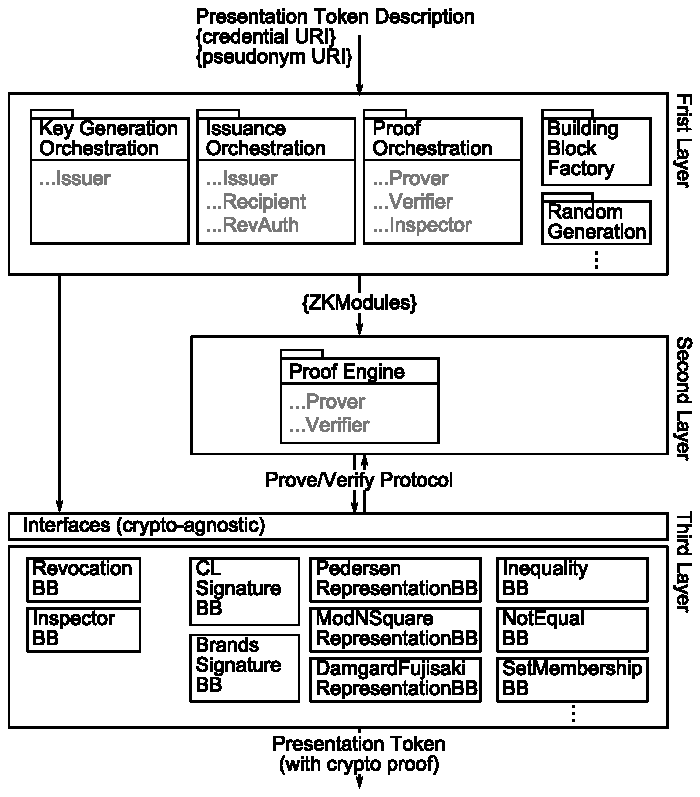
\includegraphics[width=\textwidth]{img/idmx_overview.pdf}
\caption{Visualization of the layers of the Identity Mixer architecture.
Note that singleton objects are denoted with a little box on top.}
\label{fig:overview}
\end{figure}

The second layer consists of the so called \emph{proof engine}. It receives as input a list of
ZkModules from the first layer
and generates/verifies a Fiat-Shamir zero-knowledge proof (``signature of knowledge'').
For the generation of keys, this layer is skipped and the orchestration object directly invokes the 
appropriate building block (i.e., a signature building block).


In the third layer, the abstract building blocks
only expose implementation-agnostic interfaces.
The implementations thereof know how to perform a specific cryptographic primitive, but do
not necessarily know how to interact with other primitives.
%
In general, building
blocks consist of one of more key/parameter generators, and of one
or more proof interfaces (\emph{ZkModules} factories).
%
Roughly speaking, ZkModules either (1) encapsulate the implementation of a given 
cryptographic primitive and expose a
crypto-primitive-agnostic interface to the proof engine;
or (2) have a structural role in the proof generation by indicating properties of attributes, 
relationships among attributes,
or adding messages to be signed.



\subsection{Parameter Generation}
\label{sec:arch:setup}

Let us describe the setup of parameters such as the system parameters, 
verifier parameters, or a key pair.
%
This is a two step process consisting of (1) creating a configuration template that has to 
be completed and submitted to (2) the generation of the set of parameters.
%
First, the user of the Idmx library starts by requesting a new (default) configuration template
from the crypto engine.
%
The request is forwarded to the key generation orchestration singleton object.
%
The orchestration element gathers all relevant data from the key manager 
before it
queries all relevant building blocks for the implementation specific configuration 
parameters that need to be added to the template.
%
The default configuration template is returned to the caller.


While a template is configured with default values that serve as
suggestion for a general purpose use, the actual settings must be set manually and 
in accordance with the planned use.
Note, only the general entries as well as the entries corresponding to the chosen 
implementation must be filled out in the template.
The entries
corresponding to non-chosen implementations will be ignored. 
%
We call the completed configuration template a configuration.



The second step starts with the user passing the configuration to the crypto engine, 
which forwards it to the 
orchestration object.
The latter, as in the creation of the configuration template, assembles the required  
parameters and forwards the data to the relevant 
building block corresponding to the chosen implementation.
Finally, the building block generates the requested parameters upon which they are 
returned to the requester.


\begin{figure}[htbp]
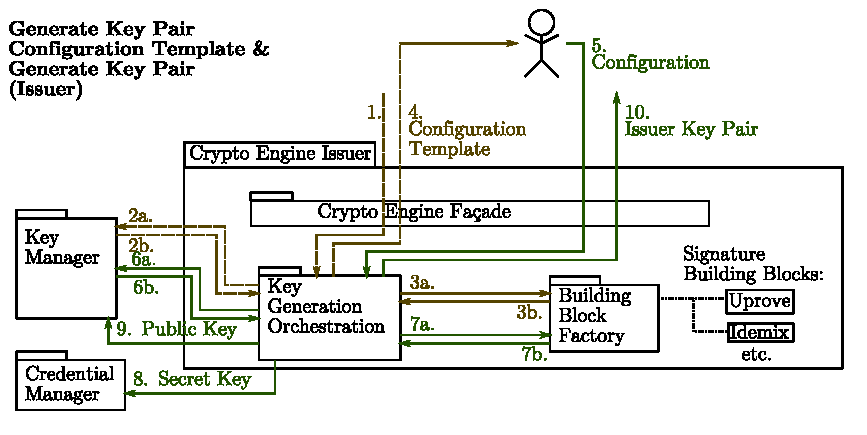
\includegraphics[width=\textwidth]{img/23.pdf}
\caption{Example of generating an issuer key pair including the creation of the 
corresponding key pair configuration template. Note that most objects in this figure 
with the exception of the concrete building blocks are singletons. This is indicated 
by the shape of their boxes.}
\label{fig:issuerkeypair}
\end{figure}

In Figure~\ref{fig:issuerkeypair} we depict the setup of an issuer key pair as an example 
of the parameter generation process. 
As mentioned before, the generation of system parameters, verifier parameters, or the
key pair of other entities is identical with the exception of a different set of
building blocks being queried. 

The user initiates with the request of a key pair configuration template (1) from the crypto 
engine.
%
Upon being forwarded to the orchestration object, the latter requests the system parameters 
from the key manager (2) as well as all signature building blocks from the building block
factory (3).
%
Further, it adds a few default entries to the configuration template, and asks each 
signature building block
in turn to add its own implementation-specific entries to the configuration template. 
The configuration
template is then returned to the user (4).


After finishing the configuration by overriding the appropriate default settings of the 
template configuration the user calls the crypto engine again with the request of generating
the parameters (5).
%
The key orchestration queries the key manager for the system parameters again (6), and the 
building
block factory for the chosen building block (7). 
It then asks the chosen building block to generate
an issuer key pair based on the configuration. 
Finally, the whole key pair is returned to the requester (10).
%
Note that the ABC4Trust adapter stores the secret key of that pair to the credential manager (8),
and the public key to the key manager (9). 


\subsection{Presentation}
\label{sec:arch:presentation}

Let us now illustrate the generation of a presentation token as depicted in 
Figure~\ref{fig:presentation}.
%
% TODO add verifier parameters
When a user wants to create a presentation token she needs to pass the presentation token
description,  a list of credential URIs, and a list of pseudonym URIs 
to the crypto engine.
%
These elements get forwarded to the proof orchestration object (1).
The proof orchestration first fetches the credentials and pseudonyms based on their URI from the
credential manager (2). 
Second, it loads the system parameters, issuer public keys, credential templates, inspector
public keys, and revocation authority public keys from the key manager (3).
Third, it queries the building block factory for the building blocks required for the presentation
token at hand (4).
For building blocks that have several implementations, the proof orchestration 
may choose a specific implementation, or it may ask the building block factory for
an implementation that is supported by the verifier.

\begin{figure}[htbp]
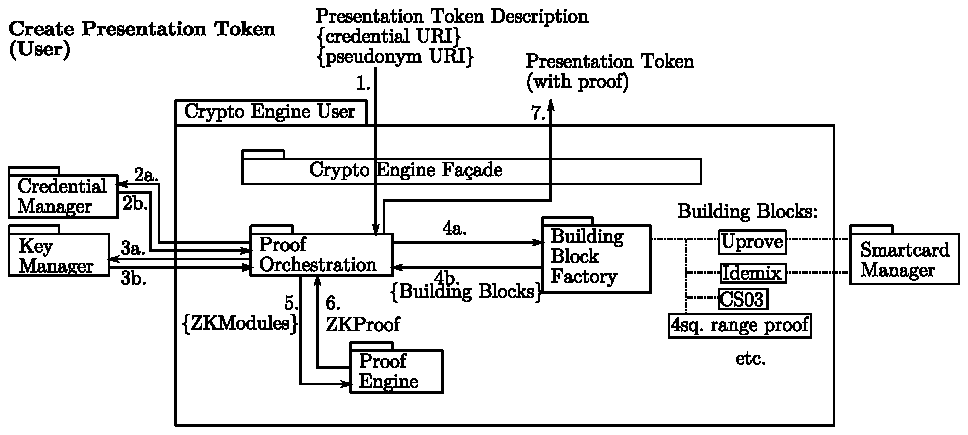
\includegraphics[width=\textwidth]{img/01.pdf}
\caption{Creation of a presentation token.}
\label{fig:presentation}
\end{figure}

These building blocks are used to generate a list of ZkModules that serve as input
to the proof engine (5).
%
The proof orchestration object will configure each ZkModule with the appropriate 
parameters such as the  keys, credentials, or pseudonyms.
The latter builds  a way of encapsulating the state needed to perform part of the overall 
zero-knowledge proof.
Note that ZkModules responsible for
proving ownership of a credential or a pseudonym may delegate part of the proof process 
to the smartcard manager.
The latter interacts with the smartcard to generate the proof elements contributed by a 
user-owned smartcard.
%
The proof engine generates a zero-knowledge proof (6) supporting the validity of the 
presentation token based on this list of ZkModules.
%
Using the proof, the orchestration object updates the presentation token description 
and then combines the former with the zero-knowledge
proof to form the final presentation token (7).




\subsection{Verification}
\label{sec:arch:verification}


Matching the presentation token to a presentation policy (as per ABC4Trust specifications) needs
to be performed before the former can be sent to the crypto engine for 
cryptographic verification (1).
%
The crypto engine forwards the
presentation token to the proof verification orchestration object, which fetches
the relevant system parameters, issuer public keys, credential
templates, inspector public keys, and revocation authority public keys from the key manager (2).


\begin{figure}[htbp]
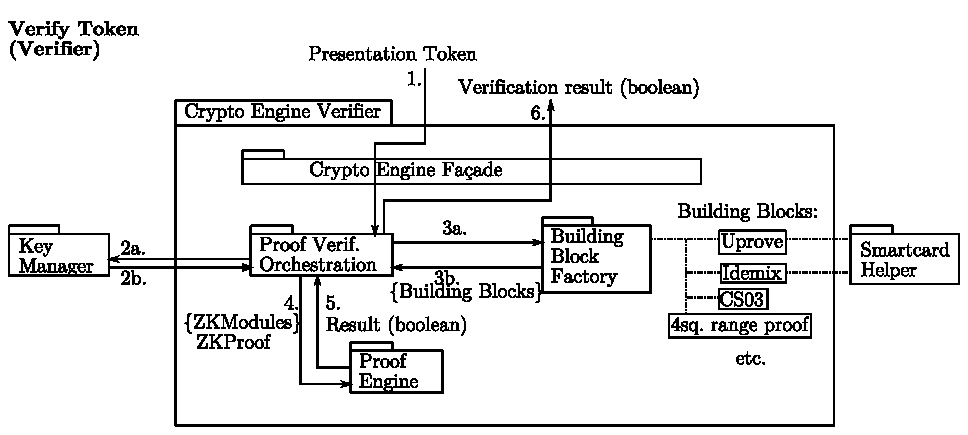
\includegraphics[width=\textwidth]{img/11.pdf}
\caption{Verification of a presentation token.}
\label{fig:verification}
\end{figure}


The verification orchestration needs to fetch the 
same set of building blocks from the building block factory (3) as the prover did.
To that end, the orchestration object uses the mechanism specification that describes the 
concrete implementations that have been chosen for each building block.
Thereafter, it can 
generate a list of ZkModules using these building blocks, where the ZkModules correspond 
to the list generated by the prover (4).
ZkModules together with the zero-knowledge proof are sent to the proof engine for 
verification.
Note that the verifier makes use of the smartcard helper, which is not connected to a smart card
but provides the functionality required to verify the part of the proof generated by a smart card.
The result of the verification (5) is then forwarded to the calling entity (6).





\subsection{Issuance}
\label{sec:arch:issuance}

We describe the issuance process in the case where no jointly-random attributes are present
and where the signing of the credential needs one round (as is the case for CL signatures).
%
Note, the issuance protocol continues for as many rounds as the used signature building block
specified and it reaches its end when the issuer specifies that it has sent the protocol 
ending message. 
%
Figure~\ref{fig:issuance1} and \ref{fig:issuance3} describe the process on the issuer's side
and Figure~\ref{fig:issuance2} and \ref{fig:issuance4} focus on the recipient of the 
credential.



\subsubsection{Issuer: Create Issuance Policy} 

On the level of the Idmx library (Fig.~\ref{fig:issuance1}), the issuance process starts with  the issuer invoking the crypto engine 
with an issuance policy and a list of issuer-set attributes (1), which 
are passed to the issuance orchestration object.
The latter saves the issuance policy and list of attributes in the state storage (2),
wraps the issuance policy in an issuance message, and returns that message to the upper layer (3).

\begin{figure}[htbp]
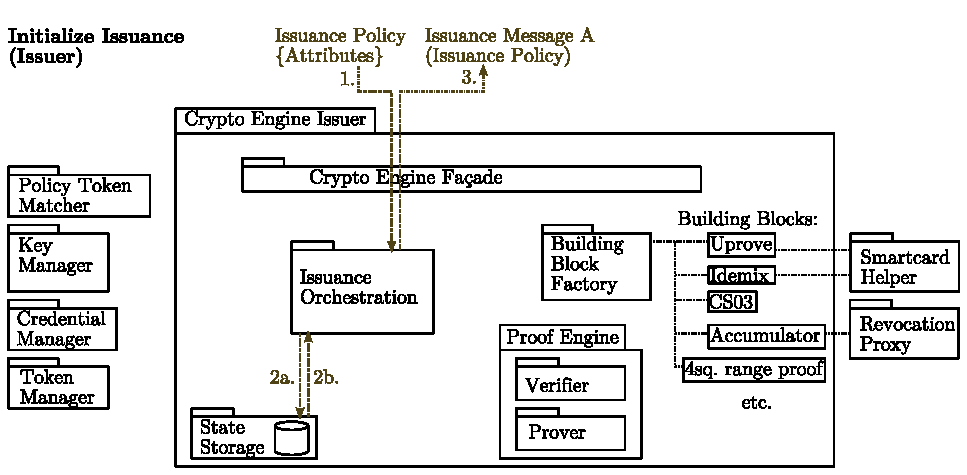
\includegraphics[width=\textwidth]{img/12.pdf}
\caption{Initiation of the issuance process on the issuer's side.}
\label{fig:issuance1}
\end{figure}




\subsubsection{Recipient: Generate Issuance Token} 

Figure~\ref{fig:issuance2} shows the recipient's side where the issuance token description, 
a list of credential URIs, a list of Pseudonym URIs, 
and the original issuance message need to be provided to the crypto engine (4).
%
These elements are forwarded to the issuance orchestration, which checks with the state storage that
the issuance context has never been seen before (5). 
Steps (6) to (10) are similar to a presentation proof (see Section~\ref{sec:arch:presentation}), with the exception of the 
issuance orchestration object additionally generating a ZkModule for carry-over from the signature building block.

\begin{figure}[htbp]
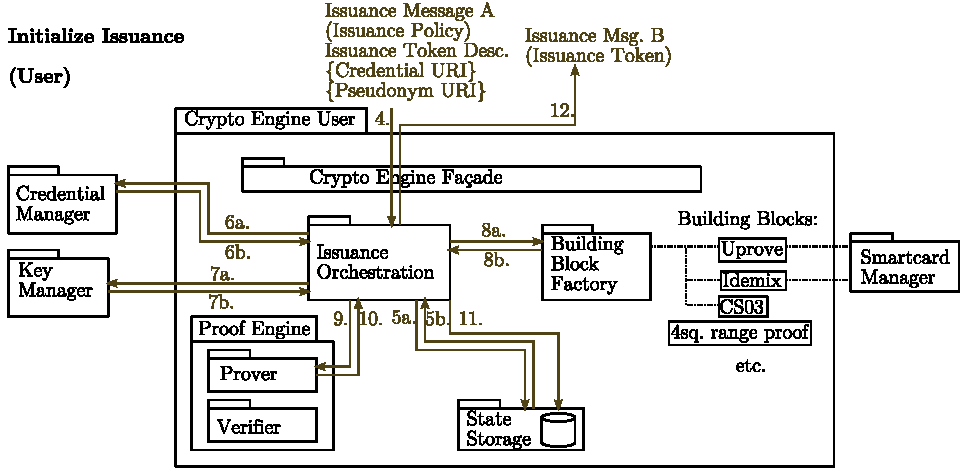
\includegraphics[width=\textwidth]{img/03.pdf}
\caption{Recipient computes an issuance token proving properties used for the credential to be issued.}
\label{fig:issuance2}
\end{figure}

After recovering the carry-over state from the proof received from the proof engine (10), orchestration 
generates an issuance token and the corresponding issuance token description, wraps the issuance token in
an issuance message, saves its current state in the state storage (11), and returns the issuance message 
to upper layer (12).




\subsubsection{Issuer: Create Signature}

The user's issuance message (containing the issuance token) is processed directly by the issuer's crypto engine.
It is passed to the issuance orchestration object (13), which recovers the state associated with the 
issuance context from the state storage (14). 
% HERE
%The issuance manager now asks the policy token Matcher from the ABC layer to check the issuance token against the
%original issuance policy (15). 
In steps (15) to (18) the issuance orchestration proceeds as the proof verification orchestration (see Section~\ref{sec:arch:verification})
to check the proof on the user's issuance token.

\begin{figure}[htbp]
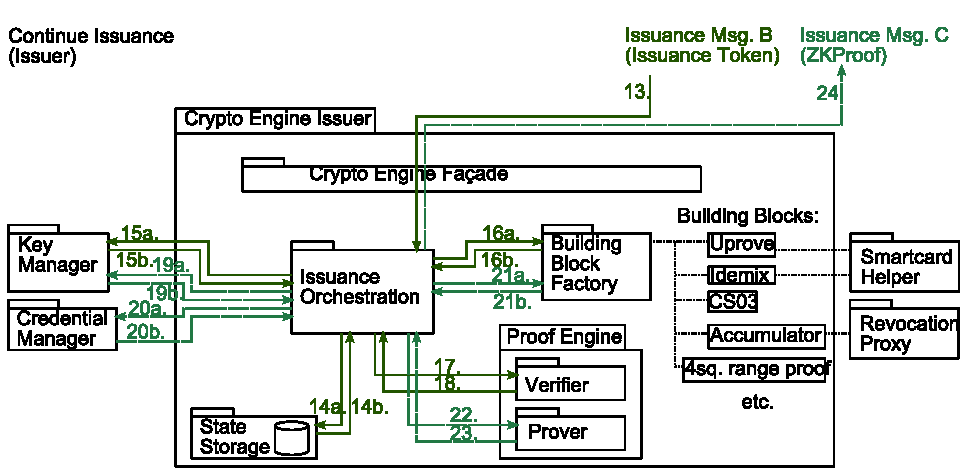
\includegraphics[width=\textwidth]{img/14a.pdf}
\caption{Issuer creates signature.}
\label{fig:issuance3}
\end{figure}


The issuance orchestration now recovers the revocation authority's public key from the key manager (19), the issuer's secret key
from the credential manager (20), and a building block for revocation of the correct implementation from the building block factory (21).
It then extracts the carry-over state from the ZkModule for carry-over and  generates a ZkModule for issuance from the
signature building block, which it initializes with the carry-over state, the issuer-set attributes, and the secret key.
If the credential that will be issued is revocable, it also generates a ZkModule for issuance from the building block for revocation.
During this step, the revocation authority will be contacted through the revocation proxy to retrieve a new revocation handle 
and the associated non-revocation evidence.
It then passes these two ZkModules to the proof engine (22).


During the proof generation, the ZkModule for signature issuance will actually perform the signature on the credential.
The issuance orchestration recovers the zero-knowledge proof from the proof engine (23). 
This zero-knowledge proof includes
the issuer's signature, the issuer-set attributes, the revocation handle, and the non-revocation evidence.
The orchestration object then queries the ZkModule for signature issuance for the list of attributes it knows about (including the revocation handle),
generates an issuance log entry.
% , and asks the ABC-layer token manager to save that log entry (26).
Finally, the zero-knowledge proof is wrapped into an issuance message, and returned to the requester (24).




\subsubsection{Recipient: Complete Signature}

The issuer's issuance message (containing the zero-knowledge proof) is processed directly by the user's crypto engine 
by passing it to the issuance orchestration object (28). 
The latter recovers the state associated with the issuance context from the state storage (29). 
It retrieves the necessary parameters, specifications and keys from the key manager (30).
Further, the orchestration loads a building block for signatures and a building block for revocation of the appropriate implementation from
the building block factory (31).

\begin{figure}[htbp]
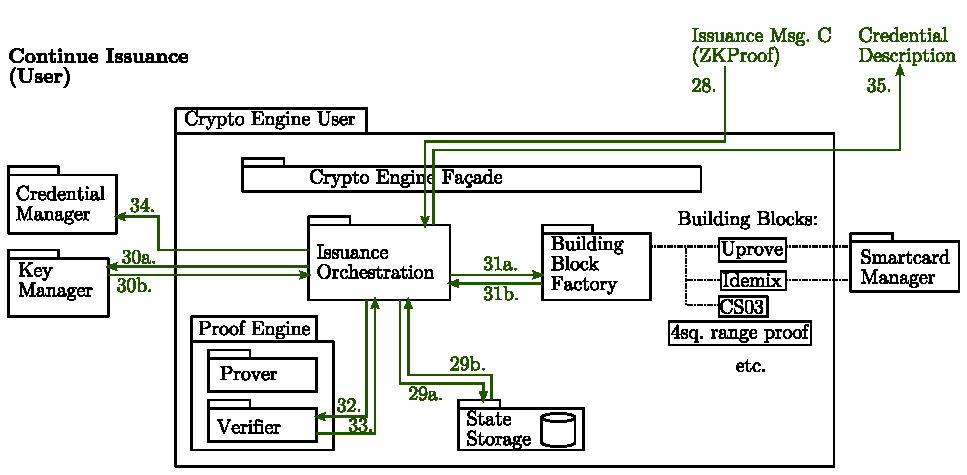
\includegraphics[width=\textwidth]{img/04.pdf}
\caption{Recipient finishes signature and stores credential.}
\label{fig:issuance4}
\end{figure}

The issuance orchestration gets a ZkModule for signature issuance from the first building block, initializing it with its
carry-over state and the issuer's public key. It also gets a ZkModule for revocation issuance from the second building block.
It then sends these two ZkModules and the zero-knowledge proof to the proof engine for verification (32).
After the issuance orchestration gets back the results of the proof verification (33), it extracts the issuance state from the
ZkModule for signature issuance. 
The issuance state can be combined with the carry-over state to recover the signed credential
and non-revocation evidence. 
The signed credential is saved in the credential manager (34). The issuance orchestration returns
the credential description to the upper layer (35).






  % from Crypto Arch (ABC4Trust)
%\section{Building a Proof}

The ZkDirector, which is a class of the proof engine, coordinates the generation of a proof.
In order to do so it uses the ZkModules that have been provided by the first layer (in particular, the 
proof orchestration). 
These modules expose an interface that encapsulates the functionality and allows the proof engine to be crypto-agnostic. 
The proof engine will execute the following steps:
\begin{itemize}
\item Initialise a ZkBuilderProver object that will keep the proof state as well as provide access to necessary elements such as the system parameters or the secrets manager.
\item Call the method \texttt{initializeModule();}  on all modules that it received as input


\end{itemize}




\section{Pedersen Representation}

In the \emph{initializeModule()} method, which is called by the ZkDirector, all attributes of this representation are registered. 
More concretely, we assume that we need  to prove knowledge of the representation:
\begin{displaymath}
C = \prod_i R_i m_i \pmod n .
\end{displaymath}
In this case, the building block registers the attributes $m_i$ specifying their bit length.
If an attribute is on an external device, the building block will not be able to compute the corresponding contribution.
Therefore, the attribute is registered as external attribute
    % to be completed
%%!TEX root =  IdmxSpecification.tex

\newcommand{\NIZK}{\operatorname{NIZK}}

\section{Example}
In this section, we show an example how an ABC4Trust Presentation
Token Description is transformed into a zero-knowledge proof specification.
%
In this example a user has two credentials: a passport and a credit card.
The user's passport credential uses CL signature technology and is bound to a smartcard,
while the credit card credential uses Brands signatures and is not bound to any smartcard.
%
Passport credentials contain the holder's name, his date of birth, and a serial number.
Credit card credentials contain the card number, the holder's name, and the status of card holder in the
credit card company's loyalty program (none, silver member, gold member, etc.).


The user wishes to book a hotel room through an ABC4Trust-enabled booking agency.
The policy of the booking agency requires the user to present a passport and a credit card.
The holder's name on both credentials must match. The passport credential must certify that
the user is over 18 years old. The booking agency also requests the user to reveal his status in
the credit card's loyalty program (to benefit from some discount). The user must
make his credit card number inspectable by a bank (with inspection grounds "payment"),
so that the booking agency can get payed. Finally, the user must sign the terms and conditions of
the booking agency in the proof.

\subsection{Notation}
By $\NIZK$ we denote a non-interactive zero-knowledge proof. In this section we only consider
zero-knowledge proofs based on the Fiat-Shamir heuristic.
We use a notation similar to the Camenisch-Stadler notation, except that we add a parameter
to $\NIZK$ representing the context to which this proof is bound. In practice the context is added to the
values to hash.
We note that in the remainder of this document we distinguish D-values (delivered to the verifier)
from N-values (values which the prover and verifier agree upon without the prover needing to
deliver the value), both of which go into the context. The notation unfortunately does not
distinguish between the two; but it should be clear from the surroundings which of the two in meant.
Revealed attributes are similar to D-values, in that they are delivered to the verifier and
part of the context, but they are treated separately in the hash computation.

For example:
\begin{align*}
\NIZK\lbrace(\alpha, \beta):
y = g^{ {\alpha}} \wedge z = g^{ {\beta}}h^{ {\alpha}}
\rbrace(\emph{ctxt})
\end{align*}
is used for proving the knowledge of the discrete logarithm of $y$ to the
base $g$, and the knowledge of a representation of $z$ to the bases $g$ and $h$ such that
the $h$-part of this representation is equal to the discrete logarithm of
$y$ to the base $g$. Furthermore the proof is bound to the context \emph{ctxt}.

\subsection{Partial Zero-Knowledge Proof and Composition}
The Proof Assembler uses Cryptogrphic Building Blocks to create so-called ZkModules (Zero Knowledge Modules),
which can be thought of as \emph{partial} zero-knowledge proofs.
The list of generated ZkModules are passed on to the Proof Engine, where \emph{conceptually} the partial zero-knowledge
proofs are combined to form the overall proof. (In practice, the Proof Engine informs the ZkModules which of their
attributes are revealed, and ensures that attributes that are equal are assigned the same R- and S-values. Otherwise
ZkModule are allowed to interact only with their child ZkModules.)

The rules for combining several partial zero-knowledge proofs are as follows:
\begin{itemize}
\item The context of the combined proof is the union of the contexts of the partial zero-knowledge proofs.
(In the sequel, for
simplicity, we sometimes do not show irrelevant values in the context, or chose to show different but related
values; this is an abuse of notation.)
\item The predicate is the logical-and of the predicates of all partial zero-knowledge proofs.
\item The witnesses in the combined proof are the union of the witnesses in the partial proofs minus
the revealed witnesses. That is, if an attribute appears as a witness in one partial proof and shows up
as a revealed attribute in another partial proof, then in the combined proof that variable shows up as
a revealed attribute only and not a witness.
\end{itemize}

\subsection{Credential Specification}
The Credential Specifications for passport and credit card credentials, as used in our example, are the following:
\subsubsection{Passport}
{
  \footnotesize
  \lstinputlisting[language=xml]{exampleCSPassport.xml}
}

\subsubsection{Credit Card}
{
  \footnotesize
  \lstinputlisting[language=XML]{exampleCSCreditCard.xml}
}

\subsection{Presentation Token Description}
The Presentation Token Description used in our example is the following:
{
  \footnotesize
  \lstinputlisting[language=XML]{examplePTD.xml}
}

\if 0
\subsection{Stored Credentials}
\subsubsection{Passport}
(Idemix)
Fullname = Bob (1114595843)
DOB = 1984-12-29 (42000)
Serial = 1234567890
Secret reference: smartcard://bob
Credential uid: cred://1234
Issuer parameters: http://example.com/isk/passport.xml
Credential spec: http://example.com/cs/passport.xml

\subsubsection{Credit Card}
(Uprove)
Number = 4349600000000005
Name = Bob (1114595843)
Status = Gold (306812052484)
credential uid: cred://0005
Issuer parameters: http://example.com/isk/cc.xml
Credential spec: http://example.com/cs/cc.xml
\fi


\subsection{Building Blocks and Top-Level ZkModules}
The Presentation Token Description and the user's choice of credentials is passed to the
Proof Assembler. The first task of the Proof Assembler is to gather Building Blocks
and use the latter to generate Prover ZkModules for the Proof Engine.
In our example, the Proof Assembler gathers the
following top-level Building Blocks and generates the following ZkModules, in order:

\begin{itemize}
\item A Message Building Block.

This block is used to generate a ZkModule identified by \texttt{msg:0} and initialized
with the contents of the \texttt{<abc:Message>} element of the Presentation Token Description.

Conceptually, if we denote the contents of the message element as $M$, the ZkModule represents
the following partial zero-knowledge proof:
\begin{align}
\NIZK\lbrace(): \operatorname{true}\rbrace(M)
\label{eq:ex:top:first}
\end{align}

\item A Signature Building Block for the passport.

The user's passport credential
is fetched from the Credential Manager. The Credential Specification and Issuer Public Key for that
credential is fetched from the Key Manager. The implementation of the Building Block (here: Camenisch-Lysyanskaya)
is selected based on the Issuer Public Key.

A Credential Specification building Block is fetched from the Building Block Factory, and a ZkModule identified by
\texttt{sig:0:cs} initialized with the Credential Specification is generated.
This ZKModule represents
the following partial zero-knowledge proof:
\begin{align}
\NIZK\lbrace(): \operatorname{true}\rbrace(\emph{cs})
\end{align}

Similarly an Issuer Parameter building block is fetched, and a ZkModule identified by
\texttt{sig:0:ip} initialized with the Issuer Public Key is generated.
This ZKModule represents
the following partial zero-knowledge proof, where \emph{ip} stands for the Issuer Parameters:
\begin{align}
\NIZK\lbrace(): \operatorname{true}\rbrace(\emph{ip})
\end{align}

The privacy-ABC signature block uses the \emph{presentation} proof interface to generate a ZkModule
identified by \texttt{sig:0} and initialized with the System and Verifier Parameters,
the Issuer Public Key, the list of attributes values of the credential $(m_1, m_2, m_3)$, the privacy-ABC signature on the attributes \emph{sig},
and an identifier of the Credential Specification $t_s$.
Furthermore, the ZkModule receives a reference to the Building Block Factory, so that it may
gather additional Building Blocks to create child ZkModules; and a reference to the External Secret Manager, so that it
may delegate some computations to the smartcard.

Conceptually, if we denote the Issuer Public Key (only the bases and modulus) as \emph{ipk},
the external secret as $x$, and the attributes as $m_1$ to $m_3$,
the ZkModule represents the following partial zero-knowledge proof:
\begin{align}
\NIZK\lbrace(m_1, m_2, m_3, x): \operatorname{Verify}(\emph{sig}, (m_1, m_2, m_3, x), t_s, \emph{ipk})\rbrace(\emph{ipk})
\end{align}
Here $t_s$ is treated as a revealed attribute, and therefore is implicitly part of the context.

\item A Signature Building Block for the credit card.

The
credential, Credential Specification and Issuer Public Key are fetched similarly as above.
The implementation of the Building Block (here: Uprove)
is selected based on the Issuer Public Key.

A Credential Specification building Block is fetched from the Building Block Factory, and a ZkModule identified by
\texttt{sig:1:cs} is generated similarily as above.
The partial zero-knowledge proof is:
\begin{align}
\NIZK\lbrace(): \operatorname{true}\rbrace(\emph{cs}')
\end{align}

Idem for the Issuer Parameter Building Block
\texttt{sig:1:ip}:
\begin{align}
\NIZK\lbrace(): \operatorname{true}\rbrace(\emph{ip}')
\end{align}

The privacy-ABC signature Building Block uses the \emph{presentation} proof interface to generate a ZkModule
identified by \texttt{sig:1} and initialized similarly as above.

Conceptually, if we denote the Credential Specification as $\emph{cs}'$, the Issuer Public Key (only the bases and group definition) as $\emph{ipk}'$,
the signature as $\emph{sig}'$, the identifier of the credential as $x_t$,
and the attributes as $m_4$ to $m_6$,
the ZkModule represents the following partial zero-knowledge proof:
\begin{align}
\NIZK\lbrace(m_4, m_5, m_6): \operatorname{Verify}(\emph{sig}', (m_4, m_5, m_6), x_t, \emph{ipk}')\rbrace(\emph{ipk}')
\end{align}
In the above, $x_t$ is considered a revealed attribute.

\item A Reveal Attribute Building Block for the status of the credit card.

This block generates a ZkModule which is initialized with the identifier of the attribute to reveal: \texttt{sig:1:2}.

Conceptually, the ZkModule declares $m_6$ as a revealed attribute.

\item An Inspection Building Block for the credit card number.

The Inspector's Public Key is fetched from
the Key Manager. The implementation of the Building Block (here: Camenisch-Shoup-03) is selected based on the
Inspector Public Key.

Similar to credentials, a Building Block for the inspector parameters \texttt{ins:1:0:inspectorKey} is added:
\begin{align}
\NIZK\lbrace(): \operatorname{true}\rbrace(\emph{ep})
\end{align}


This block uses the proof interface for \emph{verifiable encryption} to generate a
ZkModule identified by \texttt{ins:1:0} and initialized with the System and Verifier
Parameters, the Inspector Public Key and the identifier of the attribute to inspect: \texttt{sig:1:0}.
The ZkModule also receives a reference to the Building Block Factory, so that it may
gather additional Building Blocks to create child ZkModules.

Conceptually, if we denote the ciphertext as \emph{ct}, the inspections grounds as $L$, and the Inspector Public Key as
\emph{epk} (bases and modulus only), the ZkModule represents
the following partial zero-knowledge proof:
\begin{align}
\NIZK\lbrace(m_4): \emph{ct} \in \operatorname{Encrypt}(m_4, L, \emph{epk})\rbrace(\emph{ct}, L,  \emph{epk})
\end{align}
The verifiable encryption block will internally do an integer commitment to $m_4$ and an
inexact range proof that $m_4$ is between 0 and $2^{256}-1$ (inexact meaning that
the proof only guarantees that $m_4$ is in some larger range, e.g., $-2^{256+2\cdot 80}$ to $2^{256+2\cdot 80}$).

\item An Attribute Equality Building Block for the first predicate.

This block generates a ZkModule that is initialized with the identifiers of the two attributes: \texttt{sig:0:0} and \texttt{sig:1:1}.

Conceptually, the ZkModule represents
the following partial zero-knowledge proof:
\begin{align}
\NIZK\lbrace(m_1, m_5): m_1 = m_5\rbrace()
\end{align}
\item A Constant Attribute for the second operand of the second predicate.

This block generates a ZkModule that is initialized with the identifier of
the constant: \texttt{constant:1:1} and the value: \texttt{45805} (1995-05-31 under the encoding ``since1870'').

Conceptually, the ZkModule represents
the following partial zero-knowledge proof:
\begin{align}
\NIZK\lbrace(\emph{rhs}): \emph{rhs} = 45805\rbrace()
\end{align}
and \emph{rhs} is marked as a revealed attribute.

\item An Inequality Building Block for the second predicate.

The Proof Assembler chooses the implementation of the Building Block (here: 4-squares)
among the implementations supported by the verifier. The verifier included a list of
supported implementations in the Verifier Parameters. The Proof Assembler records its choice in
the Mechanism Specifications.

This block generates a ZkModule identified by \texttt{ineq:1} and initialized with the System and Verifier Parameters,
the identifiers of the two operands: \texttt{sig:0:1} and \texttt{constant:1:1}, and the operator: \texttt{LT}.
The ZkModule also receives a reference to the Building Block Factory, so that it may
gather additional Building Blocks to create child ZkModules.

Conceptually, the ZkModule represents
the following partial zero-knowledge proof:
\begin{align}
\NIZK\lbrace(m_2, \emph{rhs}): m_2 \leq \emph{rhs}\rbrace()
\end{align}
Note that the block is told whether $m_2$ originates from a group of known order or not.
If it originates from a group of known order, the Inequality Building Block would additionally
prove that $0\leq m_2$.

\item A System Parameters Building Block.

This block creates a ZkModule identified by \texttt{param:sp} and initialized with the System Parameters.

Conceptually, if we denote the system parameters as \emph{sp}, the ZkModule represents
the following partial zero-knowledge proof:
\begin{align}
\NIZK\lbrace(): \operatorname{true}\rbrace(\emph{sp})
\end{align}

\item A Verifier Parameters Building Block.

This block creates a ZkModule identified by \texttt{param:vp} and initialized
with the Verifier Parameters.

Conceptually, if we denote the system parameters as \emph{vp}, the ZkModule represents
the following partial zero-knowledge proof:
\begin{align}
\NIZK\lbrace(): \operatorname{true}\rbrace(\emph{vp})
\end{align}

\item A Presentation Token Description Building Block.

This block creates a ZkModule identified by \texttt{param:pt} and initialized
with the Presentation Token Description.

Conceptually, if we denote the presentation token description as \emph{ptd}, the ZkModule represents
the following partial zero-knowledge proof:
\begin{align}
\NIZK\lbrace(): \operatorname{true}\rbrace(\emph{ptd})
\end{align}

\item A Mechanism Specification Building Block.

This block creates a ZkModule identified by \texttt{ms} and initialized with the
Mechanism Specification that the Proof Assembler created while assembling this proof.
(Recall that the Mechanism Specification
contains, among others, the choices the Proof
Assembler made while constructing the proof.)

Conceptually, if we denote the system parameters as \emph{ms}, the ZkModule represents
the following partial zero-knowledge proof:
\begin{align}
\NIZK\lbrace(): \operatorname{true}\rbrace(\emph{ms})
\label{eq:ex:top:last}
\end{align}

\end{itemize}

The job of the Proof Engine will be to combine the partial zero-knowledge proofs of Equations
\ref{eq:ex:top:first} to
\ref{eq:ex:top:last}, to obtain the desired zero-knowledge proof:
\begin{align}
\NIZK\lbrace(
m_1, m_2, m_3, x, m_4
):& \nonumber\\
\operatorname{Verify}(&\emph{sig}, (m_1, m_2, m_3, x), t_s, \emph{ipk}) \quad \wedge \nonumber\\
\operatorname{Verify}(&\emph{sig}', (m_4, m_1, m_6), x_t, \emph{ipk}') \quad \wedge \nonumber\\
\emph{ct} &\in \operatorname{Encrypt}(m_4, L, \emph{epk}) \quad \wedge \nonumber\\
m_2 &\leq 45805 \nonumber\\
\rbrace(
M, \emph{cs}, \emph{cs}', \emph{ip}, \emph{ip}', \emph{ipk}, \emph{ipk}', &L, \emph{ct}, \emph{ep}, \emph{epk}, \emph{sp}, \emph{vp}, \emph{ms}, \emph{ptd}
)
\end{align}
Where $m_6$, $t_s$, $x_t$ and $45805$ are treated as revealed attributes.

\iffalse
\subsection{Child Building Blocks}
The two Signature ZkModules, the Verifiable Encryption ZkModule, and the Inequality ZkModule all create child ZkModules
based on Pedersen/Damgard-Fujisaki Building Blocks plus some structural Building Blocks.

\begin{itemize}
%-------------------------------------------------------------------------------
%-------------------------------------------------------------------------------
\item The CL Signature Presentation ZkModule for the passport credential.

This module is responsible for proving possession of a CL-credential (which is
bound to an external secret).

Let $\emph{ip} = (S, Z, R_0, R_1, R_2, R_3, R_s, n, \ell_e)$ be the Issuer Public Key
(where $n$ is a safe RSA modulus, $S$, $Z$ and the $R$'s are generators of the
signed quadratic residues modulo $n$, $\ell_e$ is the length of $e$). Let $t_s$ be the
identifier of the Credential Specification.
Let $x$ be the device secret, and $v_x$ be the credential secret on the device.
Let $(A, e, v)$ be the signature on the credential. Let
$(m_1, m_2, m_3)$ be the attributes on the credential. Let $e' = e - 2^{\ell_e-1}$.
Conceptually, this ZkModule re-randomizes the signature to $(A', e, v')$
and performs the following zero-knowledge proof:
\begin{align}
\label{eq:ex:cl:full}
\NIZK\lbrace(e, x, m_1, m_2, m_3, v, v_x):& \nonumber\\
Z = {A'}^e R_0^{x} R_1^{m_1}& R_2^{m_2} R_3^{m_3} R_s^{t_s} S^{v' + v_x} \pmod{n}
\rbrace(A', t_s, \emph{ip})
\end{align}

At initialization time, this ZkModules chooses a random value $r$ of appropriate
length, and re-randomizes the signature:
$A' = AS^r$; $v' = v - er$.
This ZkModule fetches the following Building Blocks from the Building Block Factory:
Damgard-Fujisaki Representation, Attribute Equality, and Issuer Parameters.
It uses these to create one Damgard-Fujisaki Representation ZkModule,
one Issuer Parameter ZkModule, and several
Attribute Equality ZkModules, as follows:

\begin{itemize}
\item It uses the Issuer Parameter Building Block to generate a ZkModule identified
by \texttt{sig:0:ip} and initialized with the Issuer Parameters $\emph{ip}$.
Conceptually, this defines the partial zero-knowledge proof:
\begin{align}
\label{eq:ex:cl:first}
\NIZK\lbrace(): \operatorname{true}\rbrace(\emph{ip})
\end{align}

\item It uses the Damgard-Fujisaki Building Block to create a ZkModule identified by \texttt{sig:0:df} and initialized
with the System and Verifier Parameters.
The bases are set to $A'$, $R_0$ (hasExternalSecret=true), $R_1$, $R_2$, $R_3$, $S$ (externalRandomizerOffset=$v'$), the modulus is set to $n$.
The identifier of the secret and the identifier of the credential for the
secret are set appropriately.
The ZkModule receives a reference to the Building Block Factory and the External Secret Manager.

This ZkModule delegates the following proof to the External Secret Manager:
\begin{align}
\NIZK\lbrace(x, v_x):
  F = R_0^x S^{v_x} \pmod{n}
\rbrace
\end{align}

The ZkModule plays a ``man in the middle'' between the External Secret Manager and the
verifier, and uses the value $F$, the T-value for $F$, and the S-values for $x$ and $v_x$,
to perform the following partial zero-knowledge proof, without knowledge of $x$ or $v_x$:
\begin{align}
\NIZK\lbrace(&a_1, x, a_2, a_3, a_4, a_5, v_x): \nonumber\\
T &= {A'}^{a_1}R_0^{x} R_1^{a_2}R_2^{a_3} R_3^{a_4} S^{a_5 + v_x} \pmod{n}
\rbrace(A', T)
\end{align}

\item Because the difference in naming between the attributes of the Damgard-Fujisaki ZkModule and the attribute
of the Signature ZkModule, it is necessary to use the Attribute Equality Building Block to generate
ZkModules specifying that the following attributes are equal:
  \begin{itemize}
  \item \texttt{sig:0:0} and \texttt{sig:0:df:2} (this corresponds to $m_1$)
  \item \texttt{sig:0:1} and \texttt{sig:0:df:3} (this corresponds to $m_2$)
  \item \texttt{sig:0:2} and \texttt{sig:0:df:4} (this corresponds to $m_3$)
  \end{itemize}
  Conceptually, these define the zero-knowledge proofs:
  \begin{align}
  \label{eq:ex:cl:last}
  &\NIZK\lbrace(m_1, a_2): m_1 = a_2\rbrace() \\
  \mbox{and }\quad&\NIZK\lbrace(m_2, a_3): m_2 = a_3\rbrace() \\
  \mbox{and }\quad&\NIZK\lbrace(m_3, a_4): m_3  = a_4\rbrace()
  \end{align}
\end{itemize}

The prover sets the value for the attributes $(a_1, a_2, a_3, a_4, a_5)$ to
$(e', m_1, m_2, m_3, v')$ in the collection phase of the
zero-knowledge proof.

The prover adds $t_s$ to the N-values.
The verifier will recompute $T$ as
$T = ZA^{-2^{\ell_e-1}}R_s^{-t_s}$.

By merging the zero-knowledge proofs defined by Equations
\ref{eq:ex:cl:first} to
\ref{eq:ex:cl:last}
and mandating that the verifier performs the check described in the previous paragraph,
we obtain the zero-knowledge proof in Equation
\ref{eq:ex:cl:full}, as desired.
%-------------------------------------------------------------------------------
%-------------------------------------------------------------------------------

\item The Uprove Signature Presentation ZkModule for the credit card credential.

This module is responsible for proving possession of a Uprove credential.

Let $\emph{ip}' = (g_0, g_1, g_2, g_3, g_t, g_p, p, \rho)$ be the Issuer Public Key (where
$p$ is a prime, and the $g$'s are generators of a prime order subgroup modulo $p$ of order $\rho$).
Let $x_t$ be the identifier of the Credential Specification. Let $\emph{ip}'$ be the Issuer
Public Key.
Let $(\bar a, h, z, c, s)$ be the signature on the credential (Uprove token), let $(m_4, m_5, m_6)$ be
the attributes of the credential, and let $\alpha = -1/\bar a$.
Conceptually, this module performs the following zero-knowledge proof:
\begin{align}
\label{eq:ex:uprove:full}
\NIZK\lbrace (\alpha, m_4, m_5, m_6): &\quad
g_0^{-1} = h^\alpha g_1^{m_4} g_2^{m_5} g_3^{m_6} g_t^{x_t} \pmod{p} \quad \wedge \nonumber\\
\operatorname{Verify}(h, z, c, s) & \quad
\rbrace(h, z, c, s, x_t, \emph{ip}')
\end{align}

(The predicate $\operatorname{Verify}$ is equivalent to checking the following proof:
$$(c, s) = \NIZK\lbrace(y_0): g_0 = g_p^{y_0} \pmod{p} \wedge z = h^{y_0} \pmod{p}\rbrace(h, z)$$
Note that this non-interactive proof was done by the issuer and uses a different challenge
than the proof generated by the Proof Assembler, so it is handled separately.)

At initialization time, this module fetches the following Building Blocks from the
Building Block Factory: Pedersen Representation, Attribute Equality, and Issuer Parameters.
It uses these to create one Pedersen Representation ZkModule,
one Issuer Parameter ZkModule, and several
Attribute Equality ZkModules, as follows:
\begin{itemize}
\item It uses the Issuer Parameter Building Block to generate a ZkModule identified
by \texttt{sig:1:ip} and initialized with the Issuer Parameters $\emph{ip}'$.
Conceptually, this defines the partial zero-knowledge proof:
\begin{align}
\label{eq:ex:uprove:first}
\NIZK\lbrace(): \operatorname{true}\rbrace(\emph{ip}')
\end{align}

\item It uses the Pedersen Building Block to create a ZkModule identified by \texttt{sig:1:rep} and initialized
with the System and Verifier Parameters.
The bases are set to $h$, $g_1$, $g_2$, $g_3$, the modulus is set to $p$, the subgroup order is set
to $\rho$.
The ZkModule receives a reference to the Building Block Factory.
(Since this ZkModule doesn't need to do computation with external secrets,
the identifier of the secret, the identifier of the credential for secret, and the external secret manager reference are all set to null.)

Conceptually, this defines the zero-knowledge proof:
\begin{align}
\NIZK\lbrace(\alpha, a_1, a_2, a_3): T = h^{\alpha} g_1^{a_1} g_2^{a_2} g_3^{a_3} \rbrace(T)
\end{align}

\item Because the difference in naming between the attributes of the Pedersen ZkModule and the attribute
of the Signature ZkModule, it is necessary to use the Attribute Equality Building Block to generate
ZkModules specifying that the following attributes are equal:
  \begin{itemize}
  \item \texttt{sig:1:0} and \texttt{sig:1:rep:1} (this corresponds to $m_4$)
  \item \texttt{sig:1:1} and \texttt{sig:1:rep:2} (this corresponds to $m_5$)
  \item \texttt{sig:1:2} and \texttt{sig:1:rep:3} (this corresponds to $m_6$)
  \end{itemize}
  Conceptually, these define the zero-knowledge proofs:
  \begin{align}
  \label{eq:ex:uprove:last}
  &\NIZK\lbrace(m_4, a_1): m_4 = a_1\rbrace() \\
  \mbox{and }\quad&\NIZK\lbrace(m_5, a_2): m_5 = a_2\rbrace() \\
  \mbox{and }\quad&\NIZK\lbrace(m_6, a_3): m_6 = a_3\rbrace()
  \end{align}
\end{itemize}

The prover sets the value for the attributes $(\alpha, m_4, m_5, m_6)$ in the collection phase of the
zero-knowledge proof, and registers the values $(h, z, c, s)$ as D-values. It also registers $x_t$
as an N-value.

The verifier will re-compute $T$ as
$T = g_0^{-1}g_t^{-x_t}$ and check that
the signature
$(h, z, c, s)$ is correct.

By merging the zero-knowledge proofs defined by Equations
\ref{eq:ex:uprove:first} to
\ref{eq:ex:uprove:last}, registering $(h, z, c, s)$ as D-values,
and mandating that the verifier performs the checks described in the previous paragraphs,
we obtain the zero-knowledge proof in Equation
\ref{eq:ex:uprove:full}, as desired.
%-------------------------------------------------------------------------------
%-------------------------------------------------------------------------------

\item The CS03 Verifiable Encryption ZkModule.

This module is responsible for encrypting an attribute using Camenisch-Shoup-03 encryption,
proving that the encryption was done properly, and delivering the
ciphertext to the verifier.

Let $\emph{ep} = (\bar n, \bar g, y_1, y_2, y_3)$ be the Inspector Public Key ($\bar n$ is a safe RSA modulus of
unknown factorization, $\bar g$ is a generator of the subgroup
of size $\varphi(\bar n)/4$ modulo $\bar n^2$, $y_1$ to $y_3$ are elements inside the subgroup generated by $\bar g$) and
let $\operatorname{hash}(\cdot, \cdot, \cdot)$ be an appropriate hash function.
Conceptually, given a message $\emph{pt}$ and a label $L$, the module chooses a random number $r$ of appropriate length and
computes:
\begin{align}
u &= {\bar g}^r \pmod{\bar n^2} \nonumber\\
\bar e &= (\bar n+1)^{\emph{pt}} y_1^r \pmod{\bar n^2} \nonumber\\
\bar v &= \operatorname{abs}\big((y_2 y_3^{\operatorname{hash}(u, \bar e, L)})^r\big) \pmod{\bar n^2}
\end{align}
It then performs the following proof:
\begin{align}
\label{eq:ex:verenc:full}
\NIZK\lbrace(\emph{pt}, r):\qquad
u &= {\bar g}^r \pmod{\bar n^2} \quad\wedge \nonumber\\
\bar e &= (\bar n+1)^{\emph{pt}} y_1^r \pmod{\bar n^2} \quad\wedge\nonumber\\
\bar v &= \operatorname{abs}\big((y_2 y_3^{\operatorname{hash}(u, \bar e, L)})^r\big) \pmod{\bar n^2} \nonumber\\
\rbrace(u, \bar e, \bar v)&
\end{align}

At initialization time, this ZkModule is not allowed to read out the value of its plaintext attribute.
That value becomes available only during the first round of the zero-knowledge proof (when the Signature
ZkModules have had the chance to provide the values of their attribute).

At initialization time, it fetches the following Building Blocks from the Building Block Factory:
ModNSquare Representation, Attribute Equality, Inspector Parameters. It uses these to create three ModNSquare ZkModules,
one Inspector Parameter ZkModule, and
several Attribute Equality ZkModules, as follows:

\begin{itemize}
\item It uses the Inspector Parameter Building Block to generate a ZkModule identified by \texttt{ins:1:0:ep} and initialized with the inspector public key \emph{ep}.
Conceptually, this defines the partial zero-knowledge proof:
\begin{align}
\label{eq:ex:verenc:first}
\NIZK\lbrace():\operatorname{true}\rbrace(\emph{ep})
\end{align}

\item It uses the ModNSquare Representation Building Block to create a ZkModule identified by \texttt{ins:1:0:u} and initialized
with the System and Verifier Parameters. The base is set to $\bar g$ (choseExponentRandomly=true, order = NPRIME),
n is set to $\bar n$.
The flag ``takeAbsoluteValue'' is not set.
The ZkModule receives a reference to the Building Block Factory.

Conceptually, this defines the zero-knowledge proof:
\begin{align}
\NIZK\lbrace(r_1): \quad u &= {\bar g}^{r_1} \pmod{\bar n^2} \rbrace(u)
\end{align}

\item It uses the ModNSquare Building Block to create a ZkModule identified by \texttt{ins:1:0:e} and initialized
with the System and Verifier Parameters. The bases are set to
$\bar n+1$ (order = N) and $\bar g$ (order = NPRIME),
n is set to $\bar n$.
The flag ``takeAbsoluteValue'' is not set.
The ZkModule receives a reference to the Building Block Factory.

Conceptually, this defines the zero-knowledge proof:
\begin{align}
\NIZK\lbrace(a_1, a_2): \quad
\bar e &= (\bar n+1)^{a_1} y_1^{a_2} \pmod{\bar n^2}
\rbrace(e)
\end{align}

\item It uses the ModNSquare Building Block to create a ZkModule identified by \texttt{ins:1:0:v} and initialized
with the System and Verifier Parameters. The base is
left unspecified for now (set to the string \texttt{ins:1:0:v:0}, order=NPRIME),
n is set to $\bar n$.
The flag ``takeAbsoluteValue'' is set.
The ZkModule receives a reference to the Building Block Factory.

Conceptually, this defines the zero-knowledge proof:
\begin{align}
\NIZK\lbrace(a_3): \quad w &= \operatorname{abs}(T_w^{a_3}) \pmod{\bar n^2} \rbrace(w)
\end{align}

\item It uses the Attribute Equality Building Block to create ZkModules that specify that the following attributes are equal:
  \begin{itemize}
    \item \texttt{ins:1:0:u:0} and \texttt{ins:1:0:e:1} (this corresponds to $r$).
    \item \texttt{ins:1:0:u:0} and \texttt{ins:1:0:v:0} (this corresponds to $r$).
    \item \texttt{ins:1:0:e:0} and the identifier of the plaintext attribute (this corresponds to $\emph{pt}$).
  \end{itemize}
  Conceptually, these define the zero-knowledge proofs:
  \begin{align}
  \label{eq:ex:verenc:last}
  &\NIZK\lbrace(r_1, a_2): r_1 = a_2\rbrace() \\
  \mbox{and }\quad&\NIZK\lbrace(r_1, a_3): r_1 = a_3\rbrace() \\
  \mbox{and }\quad&\NIZK\lbrace(a_1, \emph{pt}): a_1 = \emph{pt}\rbrace()
  \end{align}

\end{itemize}

During the \emph{first round} of the zero-knowledge proof, the Verifiable Encryption ZkModule will
begin by running the first two ModNSquare child ZkModules. It then recovers the value
$u$ and $e$ from them, and sets $T_w$:
$T_w = \operatorname{abs}(y_2 y_3^{\operatorname{hash}(u, \bar e, L)}) \pmod{\bar n^2}$. It then runs the third
ModNSquare child ZkModule.

The Verifiable Encryption ZkModule registers $u$, $e$ and $v$ as D-values.

Observe that by
setting $T_w$ to $\operatorname{abs}(y_2 y_3^{\operatorname{hash}(u, \bar e, L)})$, and merging the zero-knowledge
proofs of Equations
  \ref{eq:ex:verenc:first} to
  \ref{eq:ex:verenc:last}, we obtain the zero-knowledge proof in Equation
  \ref{eq:ex:verenc:full}, as desired.


%-------------------------------------------------------------------------------
%-------------------------------------------------------------------------------
\item The 4-Squares Inequality ZkModule.

This ZkModule is responsible for proving that the difference $\delta$ between its
right-hand-side attribute \texttt{constant:1:1} and its
left-hand-side
attribute \texttt{sig:0:1}
is larger than zero.

Conceptually, this module uses the Rabin-Shallit algorithm to find four integers $u_1, \ldots, u_4$ such
that the sum of their squares is $\delta$: $\delta = \sum_{i=1}^4 u_i^2$.
Let $(\hat n, g, h)$ be the values in the Verifier Parameters ($\hat n$ is a safe RSA modulus whose factorization
is unknown to the prover, $g$ and $h$ are generators of the signed quadratic residues modulo $\hat n$).
This block wants to perform the following proof of knowledge, for random
values $r_1, \ldots, r_5$ of appropriate length, the value $r_6 = r_5 - \sum_{i=1}^4u_ir_i$,
and delivered values $T_1, \ldots, T_5$:

\begin{align}
\label{eq:ex:rangeProof}
\NIZK\lbrace(u_1, u_2, u_3, u_4, &\emph{lhs}, \emph{rhs}, r_1, r_2, r_3, r_4, r_5, r_6): \nonumber\\
T_i &= g^{u_i} h^{r_i} \pmod{\hat n}\quad\mbox{for }i \in \lbrace1, \ldots,  4\rbrace \quad\wedge\nonumber\\
T_5 &= g^{\emph{rhs}-\emph{lhs}} h^{r_5} \pmod{\hat n}\quad\wedge\nonumber\\
T_5 &= \sum_{i=1}^4 T_i^{u_i} h^{r_6} \pmod{\hat n} \nonumber\\
\rbrace(T_1, T_2, T_3, T_4, T_5)&
\end{align}

At initialization time, this ZkModule is not allowed to read out the values of its left- and right-hand-side
arguments. These become available only during the first round of the zero-knowledge proof
(when the Signature ZkModules have had the chance to provide the values of their attributes).

At initialization time, it fetches the following Building Blocks from the Building Block Factory: Damgard-Fujisaki, Attribute Linear Combination, Attribute Equality.
It uses these to create six Damgard-Fujisaki ZkModules, one Attribute Linear Combination ZkModule,
and several Attribute Equality ZkModules, as follows:
\begin{itemize}
\item It uses the Linear Combination Building Block to create an attribute \texttt{ineq:1:delta}. That attribute
is declared as being equal to the difference between the right-hand-side attribute (\texttt{constant:1:1}) and
the left-hand-side attribute (\texttt{sig:0:1}).

Conceptually, this defines the zero-knowledge proof:
\begin{align}
\label{eq:ex:rangeProof:partial:first}
\NIZK\lbrace(\delta, \emph{lhs}, \emph{rhs}): \delta = \emph{rhs}-\emph{lhs}\rbrace()
\end{align}

\item It uses the Damgard-Fujisaki Building Block to create five ZkModules. The ZkModules are identified by
\texttt{ineq:1:df:$i$} (for $i\in\lbrace1, \ldots, 5\rbrace$, and initialized with the System and Verifier Parameters.
The bases are set to $g$ and $h$ (chooseExponentRandomly=true), the modulus to $\hat n$.
All ZkModules receives a reference to the Building Block Factory.
(Since these ZkModules don't need to do computation with external secrets
the identifier of the secret, the identifier of the credential for secret, and the external secret manager reference are all set to null.)

Conceptually, these define the zero-knowledge proofs (for $i \in \lbrace 1, \ldots, 5 \rbrace$):
\begin{align}
\NIZK\lbrace(a_i, r_i): T_i = g^{a_i} h^{r_i} \pmod{\hat n}\rbrace(T_i)
\end{align}

\item It uses the Damgard-Fujisaki Building Block to create a ZkModule identified by \texttt{ineq:1:df:6} and initialized
with the System and Verifier Parameters. The first four bases are set
to \texttt{ineq:1:df:$i$:C} for $i\in\lbrace1, \ldots, 4\rbrace$ (i.e., the not-yet-computed values of the commitments of the
first four Damgard-Fujisaki ZkModules) and the fifth base is set to $h$, the modulus to $\hat n$.
The ZkModule receives a reference to the Building Block Factory.
(Since this ZkModule doesn't need to do computation with external secrets, the same comment as above applies.)

Conceptually, this defines the zero-knowledge proof:
\begin{align}
\NIZK\lbrace(a_6, a_7, a_8, a_9, a_{10}): T_6 = T_1^{a_6} T_2^{a_7}T_3^{a_8}T_4^{a_9} h^{a_{10}} \pmod{\hat n}\rbrace(T_6)
\end{align}

\item It uses the Attribute Equality Building Block to create ZkModules that specify that the following attributes are equal:
  \begin{itemize}
    \item \texttt{ineq:1:df:1:0} and \texttt{ineq:1:df:6:0} (this corresponds to $u_1$).
    \item \texttt{ineq:1:df:2:0} and \texttt{ineq:1:df:6:1} (this corresponds to $u_2$).
    \item \texttt{ineq:1:df:3:0} and \texttt{ineq:1:df:6:2} (this corresponds to $u_3$).
    \item \texttt{ineq:1:df:4:0} and \texttt{ineq:1:df:6:3} (this corresponds to $u_4$).
    \item \texttt{ineq:1:df:5:0} and \texttt{ineq:1:delta} (this corresponds to $\delta$).
  \end{itemize}
  Conceptually, these define the zero-knowledge proofs (for $i\in\lbrace1,\ldots,4\rbrace$):
  \begin{align}
  &\NIZK\lbrace(a_i, a_{i+5}): a_i = a_{i+5}\rbrace() \\
  \mbox{and }\quad&\NIZK\lbrace(\delta, a_{10}): \delta = a_{10}\rbrace()
  \label{eq:ex:rangeProof:partial:last}
  \end{align}
\end{itemize}

The Inequality ZkModule will provide the values of $u_1, u_2, u_3, u_4$ only in the \emph{first round}
of the zero-knowledge proof: it is only then that the ZkModule is allowed to read the values of its left- and
right-hand-side attributes. During the first round, it will also recover $r_1$ to $r_5$ as the randomizers of the
first five Damgard-Fujisaki commitments, compute $r_6$, and provide the value of \texttt{ineq:1:df:6:4}
corresponding to $r_6$.

The prover registers $T_1$ to $T_5$ as D-values.
The verifier re-computes $T_6$ from $T_5$.

Observe that merging the partial zero-knowledge proofs shown in Equations
\ref{eq:ex:rangeProof:partial:first} to
\ref{eq:ex:rangeProof:partial:last}, setting
$(a_1, a_2, a_3, a_4, a_{10})$ to
$(u_1, u_2, u_3, u_4, r_6)$, and setting $T_6 = T_5$,
we obtain the zero-knowledge range proof shown in Equation
\ref{eq:ex:rangeProof}, as desired.

\item In this document we will not write out the details for the two remaining range proofs,
as they are similar to the one above.
\end{itemize}

%-------------------------------------------------------------------------------
%-------------------------------------------------------------------------------
\noindent
At this stage, the composition of all previous partial zero-knowledge proofs is the
following:
\begin{align}
\label{eq:ex:fullproof}
\NIZK\lbrace(&
% witnesses
e, x, m_1, m_2, m_3, v, v_x, \alpha, m_4, r, u_1, u_2, u_3, u_4, r_1, r_2, r_3, r_4, r_5, r_6
): \\
% predicates
Z &= {A'}^e R_0^{x} R_1^{m_1} R_2^{m_2} R_3^{m_3} R_s^{t_s} S^{v' + v_x} \pmod{n} \quad\wedge\nonumber\\
g_0^{-1} &= h^\alpha g_1^{m_4} g_2^{m_1} g_3^{m_6} g_t^{x_t} \pmod{p} \quad\wedge\nonumber\\
&\operatorname{Verify}(h, z, c, s) \quad\wedge\nonumber \\
u &= {\bar g}^r \pmod{\bar n^2} \quad\wedge \nonumber\\
\bar e &= (\bar n+1)^{m_4} y_1^r \pmod{\bar n^2} \quad\wedge\nonumber\\
\bar v^2 &= (y_2^2 y_3^{2\operatorname{hash}(u, \bar e, L)})^r \pmod{\bar n^2} \nonumber\\
T_i &= g^{u_i} h^{r_i} \pmod{\hat n}\quad\mbox{for }i \in \lbrace1, \ldots,  4\rbrace \quad\wedge\nonumber\\
T_5 &= g^{45805-m_2} h^{r_5} \pmod{\hat n}\quad\wedge\nonumber\\
T_5 &= \sum_{i=1}^4 T_i^{u_i} h^{r_6} \pmod{\hat n} \wedge \nonumber\\
0 &\leq m_4 < 2^{256} \textit{ (The latter expands to 12 representations and 20 attributes)}\nonumber\\
\rbrace(&
% context
A', h, z, c, s, u, \bar e, \bar v, T_1, T_2, T_3, T_4, T_5,
M, \emph{cs}, \emph{cs}', \emph{ip}, \emph{ip}', m_6, L, t_s, x_t, \emph{ep}, 45805, \emph{sp}, \emph{vp}, \emph{ms}
) \nonumber
\end{align}

The Proof Engine can now use standard techniques inside the Pedersen, Damgard-Fujisaki, and ModNSquare Representation ZkModules
to produce a zero-knowledge proof for Equation \ref{eq:ex:fullproof}.

%------
\fi

\subsection{Final Comments}

\paragraph{Checking Group Membership}
Although not mentioned in this section, the verifier checks that all group elements that are supposed to be signed quadratic residues
really are (note that only the verifiable encryption uses \emph{unsigned} quadratic residues).
Similarly, all group elements that are supposed to be in a subgroup of prime order are checked for subgroup membership.
        % from Crypto Arch (ABC4Trust)
%%!TEX root =  IdmxSpecification.tex

\section{Application Programming Interface (API)}
\label{sec:api}

In this section we describe the external interface of the Idmx library.
We provide access to the library using a crypto engine interface, where we offer distinct 
engines for each entity using the library.
Idmx makes use of functionality that has been implemented within the ABC4Trust project 
(published at: \url{https://github.com/p2abcengine/p2abcengine}), the so called \emph{ABC system}.
In Section \ref{sec:api:dep} we discuss the dependencies on this ABC system, which is followed by
our desctiption of the external API of the library (Sec.~\ref{sec:api:interface}).



  \subsection{Dependencies}
  \label{sec:api:dep}
  During its operation, the Idmx library will need to make calls to components 
  specified and implemented within the the ABC system.
  These components must be passed to the library when it is being initialized,
  for example by using dependency injection.
  In this section we list the components that the crypto engines of the different entities depend on.

  \subsubsection{User's Crypto Engine}
  
  Note that we provide two separate engines for the role of a recipient of a credential 
  and the role of a prover of properties about credentials.
  In many scenarios a user assumes these two roles and for this reason we describe them 
  together.
  
  \begin{itemize}
    \item CredentialManager (user)---The credential manager provides credentials and pseudonyms to the crypto engine.
    \item KeyManager---The key manager provides authenticated public keys, parameters, revocation information, and credential specifications
      to the crypto engine.
    \item RevocationProxy---The revocation authority provides the latest revocation information and can update non-revocation information
      for the crypto engine via the revocation proxy (over a secure channel).
    \item SmartcardManager---The smartcard manager helps the crypto engine conduct proofs involving device-bound credentials and pseudonyms. It
    is assumed that the smartcard manager has been properly initialized (by the credential manager) before the crypto engine is asked to
    conduct a presentation or issuance proof.
  \end{itemize}

  \subsubsection{Verifier's Crypto Engine}
  \begin{itemize}
    \item KeyManager---The key manager provides authenticated public keys, parameters, revocation information, and credential specifications
      to the crypto engine.
    \item RevocationProxy---The revocation authority provides the latest revocation information to the crypto engine via the revocation proxy (over a secure channel).
  \end{itemize}

  \subsubsection{Issuer's Crypto Engine}
  \begin{itemize}
    \item CredentialManager (issuer)---The credential manager provides the issuer's secret key to the crypto engine.
    \item KeyManager---The key manager provides authenticated public keys, parameters, revocation information, and credential specifications
      to the crypto engine. Note that fetching the revocation information may invoke the RevocationProxy (e.g., for retrieving the latest version).
    \item RevocationProxy---The revocation authority provides the latest revocation information, can update non-revocation information,
      and can provide a new revocation handle with associated non-revocation information
      to the crypto engine via the revocation proxy (over a secure channel).
%     \item TokenManager (issuer)---The token manager stores the issuance tokens that come up during the proof, and stores log entries for each issuance of
%       a credential. The crypto architecture is responsible for storing the token and log entries.
  \end{itemize}

  \subsubsection{Inspector's Crypto Engine}
  \begin{itemize}
    \item CredentialManager (inspector)---The credential manager provides the inspector's secret key to the crypto engine.
    \item KeyManager---The key manager provides authenticated public keys, parameters, revocation information, and credential specifications
      to the crypto engine.
  \end{itemize}

  \subsubsection{Revocation Authority's Crypto Engine}
  \begin{itemize}
    \item CredentialManager (revocation)---The credential manager provides the revocation authority with it's secret key. It also stores
      and retrieves the history of all revocation events, specific revocation events, and non-revocation evidences.
    \item KeyManager---The key manager provides authenticated public keys, parameters, revocation information, and credential specifications
      to the crypto engine.
  \end{itemize}


  \subsection{External API}
  \label{sec:api:interface}
  In this section we describe the external API of the different crypto engines that provide access to the Idmx library.
  We keep this section short, since most of it has already been covered by other ABC4Trust 
  documents~\cite{abc4trust:h22}.
  

  \subsubsection{User's Crypto Engine}
  
  As discussed before, a user most commonly acts as a recipient of a credential in an
  issuance protocol and thereafter she proves properties about the received credential, thereby acting
  as prover in a presentation protocol.
  Here we first describe the methods of the recipient crypto engine before detailling the prover 
  crypto engine.
  
  \paragraph{Recipient Crypto Engine}
% 	    IssuanceMessage preIssuancePresentation(IssuanceMessage issuanceMessage,
%       IssuanceTokenDescription issuanceTokenDescription, List<URI> listOfCredentialIds,
%       List<URI> listOfPseudonyms, List<Attribute> userProvidedAttributes)
	  \begin{method}
      {IssuanceMessage}
      {preIssuancePresentation}
      {
        {@in IssuanceMessage im}
        {@in IssuanceTokenDescription itd}
%         {@in VerifierParameters}
        {@in List<URI> credentialIds}
        {@in List<URI> pseudonymIds}
        {@in List<Attribute> selfClaimedAttributes}
      }
      This method does the first step in an issuance proof, namely it creates the presentation 
      token required for an advanced issuance protocol. For subsequent steps, issuanceStep() must be called.
%       For ``simple issuance'', the verifier parameters will be NULL, and all three lists empty.
      \end{method}
      
      \begin{method}
%       IssuMsgOrCredDesc issuanceStep(IssuanceMessage issuanceMessage)
      {IssuanceMessage or CredentialDescription}
      {issuanceStep}
      {
        {@in IssuanceMessage im}
      }
      This method continues the issuance protocol. The number of issuance rounds depends on the signature 
      technology and it is set by each implementation of the signature building block individually.
      \end{method}
      
      \begin{method}
%       IssuancePolicy extractIssuancePolicy(IssuanceMessage issuanceMessage)
      {IssuancePolicy}
      {extractIssuancePolicy}
      {
        {@in IssuanceMessage im}
      }
      Extracts the issuance policy from the given issuance message.
      \end{method}

  
  \paragraph{Prover Crypto Engine}

      \begin{method}
%       PresentationToken createPresentationToken(
%       PresentationTokenDescription presentationTokenDescription,
%       VerifierParameters verifierParameters, List<URI> credentialUris, List<URI> pseudonymUris)
      {PresentationToken}
      {createPresentationToken}
      {
        {@in PresentationTokenDescription ptd}
        {@in VerifierParameters}
        {@in List<URI> credentialIds}
        {@in List<URI> pseudonymIds}
      }
      This method asks the crypto engine to conduct a presentation proof.
      \end{method}
      
% TODO This method is currently not implemented. It should be ;-)
%       \begin{method}
%       {String}
%       {describePresentationToken}
%       {
%         {@in PresentationTokenDescription ptd}
%         {@in VerifierParameters}
%         {@in List<URI> credentialUris}
%         {@in List<URI> pseudonymUris}
%       }
%       This method generates a description of the proof that createPresentationToken() would create. This description
%       is intended to be shown in the user interface.
%       \end{method}
      
      \begin{method}
%       Credential updateNonRevocationEvidence(Credential credential, @Nullable URI versionOfNre,
%       boolean allowLinkableUpdate)
      {Credential}
      {updateNonRevocationEvidence}
      {
        {@in Credential credential}
        {@in @Nullable URI versionOfNre \textrm{\textit{/* If null: latest version*/}}}
        {@in boolean allowLinkableUpdate}
      }
      This method updates the non-revocation evidence in the credential to the specified version
      (or the latest version if none is specified). This method MAY refuse to update to an earlier
      version of the NRE. If the allowLinkableUpdate is false, this method MUST do the update in an
      unlikable manner.
      \end{method}  
          
      \begin{method}
%       RevocationInformation updateRevocationInformation(URI raParametersId,
%       @Nullable URI revocationInformationId)
      {RevocationInformation}
      {updateRevocationInformation}
      {
        {@in URI revocationAuthorityParametersId}
        {@in @Nullable URI revocationInformationId \textrm{\textit{/* If null: latest version*/}}}
      }
      This method returns a specific version of the revocation information (or the latest version
      if none is specified).
      \end{method}
      
      \begin{method}
%       boolean isRevoked(Credential cred)
      {boolean}
      {isRevoked}
      {
        {@in Credential cred}
      }
      This method returns true in case the credential has been revoked, and false otherwise.
      \end{method}
      
      \begin{method}
%       PseudonymWithMetadata createPseudonym(URI pseudonymId, URI scope,
%       boolean isScopeExclusive, URI secretLocation)
      {PseudonymWithMetadata}
      {createPseudonym}
      {
        {@in URI pseudonymId}
        {@in URI scope}
        {@in boolean isScopeExclusive}
        {@in URI secretLocation \textrm{\emph{/* e.g., smartcard URI*/}}}
      }
      This method creates a new pseudonym with metadata as specified in~\cite{abc4trust:h22}.
      \end{method}
      
% TODO This method is currently not there - however, the secret generation should be possible 
% also in a standalone version of the library.
%       \begin{method}
%       {Secret}
%       {createSecret}
%       {
%         {@in URI secretUriPrefix}
%       }
%       This method creates a new secret (also known as ``software smartcard'', since to the verifier,
%       it is indistinguishable from a hardware smartcard).
%       \robert{I believe that this function should be moved somewhere else, for example the smartcard manager.}
%       \end{method}
      
      
      



  \subsubsection{Verifier's Crypto Engine}
  
      \begin{method}
%       boolean verifyToken(PresentationToken presentationToken,
%       VerifierParameters verifierParameters)
      {boolean}
      {verifyToken}
      {
        {@in PresentationToken pt}
        {@in VerifierParameters vp}
      }
      This method verifies the given presentation token.
      \end{method}
      
      \begin{method}
%       RevocationInformation updateRevocationInformation(URI raParametersId,
%       @Nullable URI revocationInformationId)
      {RevocationInformation}
      {updateRevocationInformation}
      {
        {@in URI revocationAuthorityParametersId}
        {@in @Nullable URI revocationInformationId \textrm{\textit{/* If null: latest version*/}}}
      }
      This method returns a specific version of the revocation information (or the latest version
      if none is specified).
      \end{method}
      
      \begin{method}
      {VerifierParametersTemplate}
      {generateVerifierParameterConfigurationTemplate}
      {
      }
      This method generates a template for the verifier parameter configuration.
      This template will have to be filled out manually, and then given to generateVerifierParameters().
      \end{method}
      
      \begin{method}
%       VerifierParameters generateVerifierParameters(
%       VerifierParametersTemplate verifierParametersTemplate)
      {VerifierParameters}
      {generateVerifierParameters}
      {
        {@in VerifierParametersTemplate verifierParametersTemplate}
      }
      This method generates verifier parameters based on the given configuration.
      \end{method}
      
      
      



  \subsubsection{Issuer's Crypto Engine}

      \begin{method}
%       IssuanceMessageAndBoolean initializeIssuance(IssuancePolicy issuancePolicy,
%       List<Attribute> issuerProvidedAttributes, @Nullable URI context)
      {IssuanceMessageAndBoolean}
      {initializeIssuance}
      {
        {@in IssuancePolicy ip}
%         {@in VerifierParameters}
        {@in List<Attribute> issuerProvidedAttributes}
        {@in @Nullable context}
      }
      This method does the first step in an issuance proof. For subsequent steps, continueIssuance() must be called.
      If the provided context is NULL, the context will be generated at random (and be set inside the issuance message).

      This method also returns true if this is the last message of the issuance.
      This method also returns the URI of the log entry that was stored during the issuance protocol.
      \end{method}
      
      \begin{method}
%       IssuanceMessageAndBoolean issuanceStep(IssuanceMessage issuanceMessage)
      {IssuanceMessageAndBoolean}
      {issuanceStep}
      {
        {@in IssuanceMessage im}
      }
      This method continues the issuance proof and returns true if this is
      the last message of the issuance.
      This method also returns the URI of the log entry that was stored during the issuance protocol.
      \end{method}
      
      \begin{method}
%       IssuanceTokenDescription extractIssuanceTokenDescription(IssuanceMessage issuanceMessage)
      {@Nullable IssuanceTokenDescription}
      {extractIssuanceTokenDescription}
      {
        {@in IssuanceMessage im}
      }
      This method looks for an IssuanceTokenDescription inside the issuance message. It returns the issuance token, or
      NULL if none could be found.
      It is guaranteed that this method returns a non-null value before a new credential is actually issued, so that the
      upper layers may abort the issuance protocol if a certain condition is not satisfied (such as the absence of a registered pseudonym).
      \end{method}
      
      \begin{method}
%       IssuanceTokenAndIssuancePolicy extractIssuanceTokenAndPolicy(
%       IssuanceMessage issuanceMessage)
      {@Nullable IssuanceTokenAndIssuancePolicy}
      {extractIssuanceTokenAndPolicy}
      {
        {@in IssuanceMessage im}
      }
      This method looks for an IssuanceToken and an IssuancePolicy inside the issuance message. It returns those elements, or
      NULL if none could be found.
      \end{method}

% TODO maybe we should add this to the issuer's crypto engine?
% In any case the verifier and the prover both have the same code (maybe we should use an orchestration object for that?)      
%       \begin{method}
%       {RevocationInformation}
%       {updateRevocationInformation}
%       {
%         {@in URI revocationAuthority}
%         {@in @Nullable URI versionOfNre \textrm{\textit{/* If null: latest version*/}}}
%         {@in @Nullable RevocationInformation currentRevocationInformation}
%       }
%       This method returns a specific version of the revocation information (or the latest version
%       if none is specified). You may provide the current revocation information to enable a quicker update.
%       \end{method}

      \begin{method}
%       SystemParametersTemplate createSystemParametersTemplate()
      {SystemParametersTemplate}
      {createSystemParametersTemplate}
      {
      }
      This method generates a template for the system parameter configuration.
      This template will have to be filled out manually, and then given to setupSystemParameters().
      \end{method}
      
      \begin{method}
%       SystemParameters setupSystemParameters(SystemParametersTemplate systemParametersTemplate)
      {SystemParameters}
      {setupSystemParameters}
      {
        {@in SystemParametersTemplate spt}
      }
      This method generates system parameters based on the given configuration.
      \end{method}
      
      \begin{method}
%       IssuerPublicKeyTemplate createIssuerKeyPairTemplate()
      {IssuerPublicKeyTemplate}
      {createIssuerKeyPairTemplate}
      {
      }
      This method generates a template for the issuer key pair configuration.
      This template will have to be filled out manually, and then given to setupIssuerKeyPair().
      \end{method}
      
      \begin{method}
%       KeyPair setupIssuerKeyPair(SystemParameters systemParameters,
%       IssuerPublicKeyTemplate issuerParametersTemplate)
      {KeyPair}
      {setupIssuerKeyPair}
      {
        {@in SystemParameters sp}
        {@in IssuerPublicKeyTemplate ipt}
      }
      This method generates the issuer key pair based on the given configuration.
      \end{method}
      
      \begin{method}
%       VerifierParametersTemplate createVerifierParametersTemplate() 
      {VerifierParametersTemplate}
      {createVerifierParametersTemplate}
      {
      }
      This method generates a template for the verifier parameter configuration.
      This template will have to be filled out manually, and then given to setupVerifierParameters().
      \end{method}
      
      \begin{method}
%       VerifierParameters setupVerifierParameters(
%       VerifierParametersTemplate verifierParametersTemplate)
      {VerifierParameters}
      {setupVerifierParameters}
      {
        {@in VerifierParametersTemplate vpt}
      }
      This method generates verifier parameters based on the given configuration.
      \end{method}
  
      
      



  \subsubsection{Inspector's Crypto Engine}
      
      \begin{method}
%       public List<Attribute> inspect(PresentationToken presentationToken) 
      {List<Attribute>}
      {inspect}
      {
        {@in PresentationToken pt}
      }
      Inspects a presentation token.
      \end{method}
      \begin{method}
%       List<Attribute> inspect(IssuanceToken issuanceToken) 
      {List<Attribute>}
      {inspect}
      {
        {@in IssuanceToken it}
      }
      Inspects an issuance token.
      \end{method}
      \begin{method}
%       InspectorPublicKeyTemplate createInspectorPublicKeyTemplate()
      {InspectorPublicKeyTemplate}
      {createInspectorPublicKeyTemplate}
      {
      }
      This method generates a template for the inspector's key pair configuration.
      This template will have to be filled out manually, and then given to generateKeyPair().
      \end{method}
      \begin{method}
%       KeyPair setupInspectorKeyPair(SystemParameters systemParameters,
%       InspectorPublicKeyTemplate template)
      {KeyPair}
      {setupInspectorKeyPair}
      {
        {@in SystemParameters sp}
        {@in InspectorPublicKeyTemplate ipt}
      }
      This method generates the inspector's key pair based on the given configuration.
      \end{method}

\robert{Do we need interfaces to prove that an inspection was done properly (with a zero-knowledge proof)?}
 
      
      



  \subsubsection{Revocation Authority's Crypto Engine}
      
      \begin{method}
%       NonRevocationEvidence newRevocationHandle(URI raParametersId,
%       URI nonRevocationEvidenceId, List<Attribute> attributes)
      {NonRevocationEvidence}
      {newRevocationHandle}
      {
        {@in URI revocationAuthorityParamtersId}
      }
      This method is intended to be called though the revocation proxy. This method generates
      a new revocation handle and the corresponding non-revocation evidence.
      This method additionally returns the URI of the latest revocation information.
      \end{method}
      
      \begin{method}
%       RevocationInformation updateRevocationInformation(URI raParametersUID,
%       @Nullable URI revocationInformationUID,
%       @Nullable RevocationInformation currentRevocationInformation)
      {RevocationInformation}
      {updateRevocationInformation}
      {
        {@in URI revocationAuthorityParametersId}
        {@in @Nullable URI revocationInformationId \textrm{\textit{/*If null: latest version*/}}}
%         {@in @Nullable RevocationInformation currentRI}
      }
      This method is intended to be called through the revocation proxy. This method returns
      a specific version of the revocation information.
      \end{method}

%       \begin{method}
%       {NreUpdateResponse}
%       {updateNonRevocationEvidence}
%       {
%         {@in URI revocationAuthorityUri}
%         {@in @Nullable URI previousVersionOfNRE \textrm{\textit{/*If null: don't update; generate new*/}}}
%         {@in @Nullable URI versionOfNRE \textrm{\textit{/*If null: latest version*/}}}
%         {@in NreUpdateRequest request}
%       }
%       This method is intended to be called through the revocation proxy. This method helps the caller
%       update a non revocation evidence to a specific version (or the latest version).
%       The structure of the request and the return value are implementation-specific.
%       \end{method}
      
      \begin{method}
%       URI revoke(URI revocationAuthorityId, BigInt revocationHandleValue)
      {URI}
      {revoke}
      {
        {@in URI revocationAuthorityParametersId}
        {@in BigInt revocationHandle}
      }
      This method revokes the specified revocation handle, and returns the URI of the latest
      revocation information.
      \end{method}
      
      \begin{method}
%         RevocationHistory getRevocationHistory(URI raParametersId)
      {RevocationHistory}
      {getRevocationHistory}
      {
        {@in URI revocationAuthorityParametersId}
      }
      Returns the revocation history.
      \end{method}
      
      \begin{method}
%       RevocationAuthorityPublicKeyTemplate createRevocationAuthorityPublicKeyTemplate()
      {RevocationAuthorityPublicKeyTemplate}
      {createRevocationAuthorityPublicKeyTemplate}
      {
      }
      This method generates a template for the revocation authority's key pair configuration.
      This template will have to be filled out manually, and then given to setupRevocationAuthorityKeyPair().
      \end{method}
      
      \begin{method}
%       KeyPair setupRevocationAuthorityKeyPair(SystemParameters systemParameters,
%       RevocationAuthorityPublicKeyTemplate template)
      {KeyPair}
      {setupRevocationAuthorityKeyPair}
      {
        {@in SystemParameters sp}
        {@in RevocationAuthorityPublicKeyTemplate rapt}
      }
      This method generates the revocation authority's key pair based on the given configuration.
      \end{method}
      
     
             % from Crypto Arch (ABC4Trust)
%%!TEX root =  IdmxSpecification.tex

\section{Building Blocks}

In this Section we describe the cryptographic building blocks supported
by the Idmx library, and list their interfaces.
We start by describing interfaces that are shared by
multiple building blocks. 
Section~\ref{sec:blocks:common} we outline the interfaces that are shared among most 
building blocks.
In Section~\ref{sec:blocks:major} we describe
the major building blocks, which are \emph{abstract} interfaces, and
list their concrete realization in Section~\ref{sec:blocks:major:impl}.
Further, Section~\ref{sec:blocks:helper} we describe
the helper building blocks, which are used as ``subroutines'' by the major blocks.
Finally, in Section~\ref{sec:blocks:structural} we describe the structural
building blocks, whose role it is to configure the zero-knowledge proof.

%!TEX root =  IdmxSpecification.tex

  \subsection{Common Interfaces}
  \label{sec:blocks:common}
  In this section, we describe the interfaces that are shared by most
  building blocks. Certain blocks require system parameters, keys, or verifier
  parameters to function; here we describe the interface through which these
  blocks can generate these parameters and keys. Building blocks that take part
  in a zero-knowledge proof have one or several proof interfaces (ZkModules).

    \subsubsection{Interface for all building blocks}
    \label{sec:intf:all}
    All general building blocks must implement the following method:
      \begin{getter}{URI}{getBuildingBlockId}
      Returns the name of the building block.
      This name should start with \identifier{}.
      For example, the signature building block will have the building block 
      id: \identifier{sig}.
      \end{getter}
    \subsubsection{Interface for all implementation building blocks}
    \label{sec:intf:major}
%     All major building blocks must contain the following abstract method:
      \begin{getter}{URI}{getImplementationId}
      Returns the name of the current implementation of the building block.
      This name should start with the identifier of a block and adds the
      appropriate suffix for this implementation. For example, the CL signature
      building block extending the general signature building block will
      have the implementation id: \identifier{sig:cl}.
      \end{getter}


    \subsubsection{System parameter generator}
    \label{sec:intf:syspargen}
    System parameters must be generated before the system is deployed, and
    should be distributed to all clients in the system.
    System parameters are generated in several steps. 
    First, a template of a configuration file is generated. 
    This template consists of a list of fields together with a description. 
    Each building block that implements the
    system parameter interface may contribute to this list of fields.
    Second, the client has to specify a value for each of the fields
    in the configuration template, thus creating a configuration file.
    Third, the configuration file is parsed by all the building
    blocks that contributed to the configuration template, 
    and a list of system parameters is created based on
    the configuration file.

    Building blocks that need to create their own system parameters must implement
    the following methods:
      \begin{method}
      {void}
      {generateSystemParameterConfigurationTemplate}{{@inout Set<FieldDescription> configurationFileTemplate}}
      This method may add fields (and a human friendly description) to the system parameter configuration file.
      \end{method}
      \begin{method}
      {void}
      {generateSystemParameters}
      {
        {@in Map<FieldDescription, Value> configurationFile}
        {@inout Map<Field, Value> systemParameters}
      }
      This method generates system parameters based on the configuration file provided by the user.
      The method should only read fields in the configuration file that it added with the
      function generateSystemParameterConfigurationTemplate earlier.
      \end{method}

    \subsubsection{Key pair generator}
    \label{sec:intf:keygen}
    Key pairs are generated by each issuer, each revocation authority, and each inspector in the
    system. The public key of that pair must be distributed to all clients before they are able
    to interact with the entity which generated the key pair.
    Key pairs are generated in a manner similar to the system parameters:
    first a configuration template is generated by the entity wishing to generate a key pair,
    second the template is completed (manually) by the entity to yield the configuration file, third the
    configuration file is parsed and the key pair is generated.

    Building blocks that need to generate a key pair must implement the following methods:
      \begin{getter}{Set<FieldDescription>}{generateKeyPairConfigurationTemplate}
      This method generates the key pair parameter configuration template (which consists of a list of
      field names and their human friendly descriptions).
      \end{getter}
      \begin{method}
      {KeyPair}
      {generateKeyPair}
      {
        {@in Map<Field, Value> systemParameters}
        {@in Map<FieldDescription, Value> configurationFile}
      }
      This method generates a key pair (consisting of a public key and a secret key)
      based on the configuration file provided by the user and the
      current system parameters.
      \end{method}

    \subsubsection{Verifier parameter generator}
    \label{sec:intf:verpargen}
    Verifier parameters may be generated by each verifier in the system, and are
    transmitted to the prover together with the policy.
    Verifier parameters are generated in a manner similar to the system parameters and key pairs:
    first a configuration template is generated by the verifier, second it is
    completed (manually) by the verifier to yield the configuration file, third the
    configuration file is parsed and the verifier parameters are generated.

    Building blocks that need to create verifier parameters must implement the
    following methods:
      \begin{method}{void}{generateVerifierParameterConfigurationTemplate}{{@inout Set<FieldDescription> configurationFileTemplate}}
      This method may add fields (and a human friendly description) to the verifier parameter configuration file.
      \end{method}
      \begin{method}
      {void}
      {generateVerifierParameters}
      {
        {@in Map<Field, Value> systemParameters}
        {@in Map<FieldDescription, Value> configurationFile}
        {@inout Map<Field, Value> verifierParameters}
      }
      This method generates verifier parameters based on the configuration file provided by the user and the
      current system parameters.
      The method should only read fields in the configuration file that it added with the
      function generateVerifierParameterConfigurationTemplate earlier.
      \end{method}

    \subsubsection{Proof Interface}
    \label{sec:intf:proof}
    All building blocks that participate in a zero-knowledge proof must implement the following
    tuple of ZkModule factories (ZkModule-generating methods); these ZkModules are used as input
    to the proof engine.
    Building blocks that have several proof interfaces will
    implement several of these triples, each one with a different suffix \texttt{\emph{XXX}}.
    Building blocks may freely choose the arguments of the methods below (however in order to
    guarantee an implementation-agnostic code, different implementations
    of the same building block must have exactly the same method names and arguments).
      \begin{method}
      {ZkModuleProver}
      {getZkModuleProver\emph{XXX}}
      {
        {\textrm{\textit{Each building block can choose the arguments of this method}}}
      }
      This method create a new ZkModuleProver object. This object: (1) encapsulates the state of the current
      building block implementation that is needed for
      generating a zero-knowledge proof; and (2) exposes a unified interface to the proof engine.
      We describe ZkModuleProver in more detail below.
      \end{method}
      \begin{method}
      {ZkModuleVerifier}
      {getZkModuleVerifier\emph{XXX}}
      {
        {\textrm{\textit{Each building block can choose the arguments of this method}}}
      }
      This method create a new ZkModuleVerifier object. This object: (1) encapsulates the state of the current
      building block implementation that is needed for
      verifying a zero-knowledge proof; and (2) exposes a unified interface to the proof engine.
      We describe ZkModuleVerifier in more detail below.
      \end{method}
      % \begin{method}
      % {ZkModuleDescriber}
      % {getZkModuleDescriber\emph{XXX}}
      % {
        % {\textrm{\textit{Each building block can choose the arguments of this method}}}
      % }
      % This method create a new ZkModuleDescriber object. This object: (1) encapsulates the state of the current
      % building block implementation that is needed for
      % describing a zero-knowledge proof; and (2) exposes a unified interface to the proof engine.
      % We describe ZkModuleDescriber in more detail below.
      % \end{method}

    \subsubsection{ZkModules}
    ZkModuleProver and ZkModuleVerifier are abstract classes that expose a unified interface to
    the proof engine for conducting Fiat-Shamir zero-knowledge proofs and verifying them.
    The concrete instantiation of these modules encapsulate implementation specific state.

    All three ZkModules must implement the following methods:
    \begin{getter}
    {String}
    {getIdentifier}
    Returns the unique identifier of this instance. This identifier can be freely chosen at runtime,
    must be unique throughout the proof, and
    it must be guaranteed that the prover and the verifier agree on the same identifier.
    \end{getter}
    \begin{getter}
    {String}
    {getBuildingBlockId}
    Returns the name of the building block that generated this instance.
    This name should start with \identifier{b:}.
    \end{getter}
    \begin{getter}
    {String}
    {getImplementationId}
    Returns the name of the specific implementation of the building block that generated this instance.
    For major building blocks (which admit more than one implementation), this name should start with \identifier{i:}.
    For building blocks which admit only one implementation, the return value
    must be the same as for getBuildingBlockId().
    \end{getter}


    \paragraph{ZkModuleProver}
%     \subsubsubsection{ZkModuleProver}
    \label{sec:intf:zkmoduleprover}
    When a proof is being conducted, each of the following methods will be called (in the order
    given below) on each of the ZkModuleProver participating in the proof.
    In all of these method calls, the ZkModuleProver is given a reference to ZkBuilder with
    which it is supposed to interact. The ZkBuilder is responsible for centralizing the
    actions of all ZkModules.
    (We note here that there is exactly one ZkBuilder that is active during the proof, and that
    the ZkModuleProver is given a reference to a ``firewalled'' version of the former, which restricts the
    methods that can be called).
    \begin{method}
    {void}
    {initializeModule}
    {
      {@ref ZkBuilderStateInitialize zkBuilder}
    }
    Notify the zkBuilder of all attributes (including temporary variables) that it will use during the proof.
    Notify the zkBuilder which attribute values this ZkModule requires from other ZkModules, and which attribute values this ZkModule
    will provide for other ZkModules (the modules will be topologically sorted after this function call).
    The method may declare that an attribute is to be revealed, or that two attributes are equal.

    The ZkBuilderStateInitialize ``firewall'' allows the following methods to be called on the zkBuilder:
      \begin{itemize}
      \item void registerAttribute(String name, Range r, boolean isExternal)---indicates that this module will use the
       given attribute during the proof.
       The module must specify the range of acceptable values for this attibutes, to assist the proof engine in
       choosing an R-value (see §\ref{zkproof:terminology}) of the correct size.
       The isExternal flag is used for attributes that are on external devices (such as
       smartcards).
      \item void requiresAttributeValue(String name)---indicates that this module needs to know the value of the given attribute
       in the collectAttributesForProof() function. Modules will be topologically sorted to guarantee that this value is available.
      \item void providesAttributeValue(String name)---indicates that this module will provide the value of the given attribute
       later, namely when the module is called again though the collectAttributesForProof() function
       (using the attribute values it required with requiresAttributeValue).
       In case of circular dependency an error is raised. If this
       module knows the value of the attribute now already, it should call setValueOfAttribute
       immediately instead.
      \item void attributeIsRevealed(String name)---indicates that the given attribute must be revealed by the proof engine.
      \item void attributesAreEqual(String attributeName1, String attributeName2)---indicates that the given attribute are
        to be treated as one and the same by the proof engine. This method will fail if an external and a non-external attribute
        are passed as arguments.
      \item void attributeLinearCombination(String attributeName1, BigInteger constant, List<StringAndBigInteger> attributeAndMultiplier)---
        indicates that the given attribute is equal to a linear combination of the attributes in the list plus a constant.
        The proof engine will choose the R-values of all attributes accordingly. In case of a circular dependency,
        an error is raised.
      \item void setValueOfAttribute(String name, BigInteger value, ResidueClass rc)---sets the value of the given attribute, so that the
        proof engine can share this value with other modules. The residue class informs the proof engine
        whether the attribute is: (1) an integer in the range 0...q (where q is the subgroup order),
        (2) any integer, (3) a value modulo q, (4) a value modulo another value, or (5) unspecified.
        This information is used by the range proof module to decide whether it is necessary
        to conduct a proof that the attribute is larger than 0 or smaller than q.
        If multiple residue classes are specified (even across blocks), then the
        proof engine will intelligently combine the choices.
      \item void markAsSignatureBuildingBlock()---marks the current ZkModule as being a signature
      building block. This is important when computing the challenge: indeed the hash
      contribution of the first signature
      building block is treated specially in order to guarantee compatibility with the U-Prove
      specification.
      \item DeviceProofSpecification getDeviceProofSpecification()---returns an object that
      the ZkModule can use to ask the external device (smartcard) to do a certain zero-knowledge proof.
      \end{itemize}
    \end{method}
    \begin{method}
    {void}
    {collectAttributesForProof}
    {
      {@ref ZkBuilderStateCollect zkBuilder}
    }
    For all attributes for which this module called providesAttributeValue(), this method
    must provide the value of that attribute to the ZkBuilder. This module may query the attribute
    value for all attributes for which this method called requiresAttributeValue().
    (The modules were topologically sorted prior to this function being called.)

    The ZkBuilderStateCollect ``firewall'' allows the following methods to be called on the zkBuilder:
      \begin{itemize}
      \item boolean isRevealedAttribute(String name)
      \item BigInteger getValueOfAttribute(String name)---may only call this method if requiresAttributeValue() has been
       called in the previous round on the same attribute.
      \item void setValueOfAttribute(String name, BigInteger value, ResidueClass rc)---you must call this method for all attributes
        for which you called providesAttributeValue() in the previous round.
      \item ResidueClass getResidueClassOfAttribute(String name)
      \item DeviceProofSpecification getDeviceProofSpecification()
      \end{itemize}
    \end{method}
    \begin{method}
    {void}
    {firstRound}
    {
      {@ref ZkBuilderStateFirst zkBuilder}
    }
    Ask the builder which attributes are revealed (and recover their value) and
    which attributes are unrevealed (and recover the R-value (randomizer) associated with the attribute).
    Generate T-values (first message of a $\Sigma$-protocol, see §\ref{zkproof:terminology}) for each equations, generate D-values (values delivered to the verifier),
    register N-values (context values that both the prover and verifier know, see §\ref{zkproof:terminology}), and
    generate nonce commitments. Send these to the builder.

    The ZkBuilderStateFirst ``firewall'' allows the following methods to be called on the zkBuilder:
      \begin{itemize}
      \item boolean isRevealedAttribute(String name)
      \item boolean isValueOfAttributeAvailable(String name)
      \item BigInteger getValueOfAttribute(String name)
      \item ResidueClass getResidueClassOfAttribute(String name)
      \item BigInteger getRValueOfAttribute(String name)
      \item GroupElement getDValueAsGroupElement(String name)---at this stage, this method may only be called for
        D-values (values delivered to the verifier, see §\ref{zkproof:terminology}) that were generated by any of the (transitive closure) of the children of the top-level module
        this module belongs to, and only if the top-level module guarantees that the D-value has already been
        added at the point this method is called. This is because 1) the proof engine does not provide any guarantees
        on the order in which the top-level modules get called, and 2) the D-value must be available before this
        method is called.
      \item void addDValueAsGroupElement(String name, GroupElement value)
      \item void addDValueAsObject(String name, byte[] value, byte[] hashContribution)
      \item void addNValue(String name, byte[] hashContribution)
      \item void addTValueForEquation(String name, GroupElement tValue)
      \item void setHashContributionOfBuildingBlock(byte[] hashContribution)---Manually set the
      hash contribution of the building block instead of letting it be computed by
      the proof engine based on the T-,D-,and N-value and the revealed attributes. Use with caution.
      \item DeviceProofCommitment getDeviceProofCommitment()---Obtain the T-values computed by
      the external devices (smartcards).
      \end{itemize}
    \end{method}
    \begin{method}
    {void}
    {secondRound}
    {
      {@ref ZkBuilderStateSecond zkBuilder}
    }
    Recover the value of the nonce commitments, and the challenge from the zkBuilder.
    Generate the S-value (third message of a $\Sigma$-protocol, see §\ref{zkproof:terminology}) for all external attributes, and send
    them to the builder.

    The ZkBuilderStateSecond ``firewall'' allows the following methods to be called on the zkBuilder:
      \begin{itemize}
      \item BigInteger getChallenge()
      \item boolean isRevealedAttribute(String name)
      \item boolean isValueOfAttributeAvailable(String name)
      \item BigInteger getValueOfAttribute(String name)
      \item ResidueClass getResidueClassOfAttribute(String name)
      \item BigInteger getRValueOfAttribute(String name)
      \item GroupElement getDValueAsGroupElement(String name)
      \item byte[] getDValueAsObject(String name)
      \item void setSValueForAttribute(String name, BigInteger sValue)---Ideally this function should be called
        for external attributes only (e.g., attributes on smartcards).
      \item DeviceProofResponse getDeviceProofResponse()---Obtain the S-values computed
      by the external devices (smartcards).
      \end{itemize}
    \end{method}

\paragraph{ZkModuleVerifier}
%     \subsubsubsection{ZkModuleVerifier}
    \label{sec:intf:zkmoduleverifier}
    When a proof is being verified, each of the following methods will be called (in the order
    given below) on each of the ZkModuleVerifier participating in the proof verification.
    In all of these method calls, the ZkModuleVerifier is given a reference to a ZkVerifier with
    which it is supposed to interact. The ZkVerifier is responsible for centralizing the
    actions of all ZkModules.
    (We note here that there is exactly one ZkVerifier that is active during the proof, and that
    the ZkModuleVerifier is given a reference to a ``firewalled'' version of the former, which restricts the
    methods that can be called).
    \begin{method}
    {void}
    {collectAttributesForVerify}
    {
      {@ref ZkVerifierStateCollect zkVerifier}
    }
    Notify the zkVerifier of all attributes (including temporary variables) that will be used during the proof.
    The method may declare that an attribute is to be revealed, that two attributes are equal, or enforce
    a particular value of an attribute.

    The ZkVerifierStateCollect ``firewall'' allows the following methods to be called on the zkBuilder:
      \begin{itemize}
      \item void registerAttribute(String name, Range r, boolean isExternal)
      \item void attributeIsRevealed(String name)
      \item void setResidueClassOfAttribute(String name, ResidueClass rc)
      \item void enforceValueOfAttribute(String name, BigInteger value)
      \item void attributesAreEqual(String attributeName1, String attributeName2)
      \item void attributeLinearCombination(String attributeName1, BigInteger constant, List<StringAndBigInteger> attributeAndMultiplier)
      \item byte[] getDValueAsObject(String name)
      \end{itemize}
    \end{method}
    \begin{method}
    {boolean}
    {verify}
    {
      {@ref ZkBuilderStateFirst zkBuilder}
    }
    Ask the zkVerifier which attributes are revealed (and recover their value) and
    which attributes are unrevealed (and recover their S-value), recover D-values,
    recover the challenge.
    Re-compute the T-values for each equation, check the hash contribution of the D-values,
    and perform implementation specific-checks.
    Return false if any of the implementation-specific checks fail.

    The ZkBuilderStateFirst ``firewall'' allows the following methods to be called on the zkBuilder:
      \begin{itemize}
      \item BigInteger getSValueOfAttribute(String name)
      \item GroupElement getDValueAsGroupElement(String name)
      \item byte[] getDValueAsObject(String name)
      \item boolean isRevealedAttribute(String name)
      \item BigInteger getValueOfRevealedAttribute(String name)
      \item void checkValueOfAttribute(String name, BigInteger value)
      \item ResidueClass getResidueClassOfAttribute(String name)
      \item BigInteger getChallenge()
      \item void checkHashContributionOfBuildingBlock(byte[] hashContribution)---Use only if
        the prover set a custom hash contribution.
      \item void checkHashContributionOfDValue(String name, byte[] hashContribution)---This method must
        be called for each non-integer D-value in the proof, otherwise an error is raised.
      \item void checkNValue(String name, byte[] hashContribution)---This method must be called for
        each N-value that was added to the proof, otherwise an error is raised.
      \item void checkHashContributionOfDValue(String name, byte[] hashContribution)---This method
        must be called for each D-Value that has a custom hash contribution.
      \item void checkTValue(String name, GroupElement tValue)---This method must be called
        for each T-value in the proof, otherwise an error is raised.
      \end{itemize}
    \end{method}


% \item[ZkModuleDescriber]
% %     \subsubsubsection{ZkModuleDescriber}
%     When a proof is being described, each of the following methods will be called (in the order
%     given below) on each of the ZkModuleDescriber participating.
%     In all of these method calls, the ZkModuleDescriber is given a reference to ZkDescriber with
%     which it is supposed to interact. The ZkDescriber is responsible for centralizing the
%     actions of all ZkModules.
%     (We note here that there is exactly one ZkDescriber that is active during the proof, and that
%     the ZkModuleDescriber is given a reference to a ``firewalled'' version of the former, which restricts the
%     methods that can be called).
%     \begin{method}
%     {void}
%     {initializeForDescribe}
%     {
%       {@ref ZkDescriberStateInitialize zkDescriber}
%     }
%     This method is identical to the corresponding method of ZkModuleProver, except that
%     this module may also register ``human friendly'' attribute values.
% 
%     The ZkDescriber allows also the following function to be called:
%     \begin{itemize}
%       \item void setHumanFriendlyValueOfAttribute(String name, String humanFriendlyValue)
%     \end{itemize}
%     \end{method}
%     \begin{method}
%     {void}
%     {collectAttributesForDescribe}
%     {
%       {@ref ZkDescriberStateCollect zkDescriber}
%     }
%     This method is identical to the corresponding method of ZkModuleProver, except that
%     this module may also register ``human friendly'' attribute values.
% 
%     The ZkDescriber allows also the following function to be called:
%     \begin{itemize}
%       \item void setHumanFriendlyValueOfAttribute(String name, String humanFriendlyValue)
%     \end{itemize}
%     \end{method}
%     \begin{method}
%     {void}
%     {describeProof}
%     {
%       {@ref ZkDescriberStateDescribe zkDescriber}
%       {@inout ProofDescription description}
%     }
%     Ask the builder which attributes are revealed (and recover their value) and
%     which attributes are unrevealed.
%     Modifies the given proof description to add what the corresponding zkModuleProver does in the proof.
% 
%     The ZkBuilderStateDescribe ``firewall'' allows the following methods to be called on the zkBuilder:
%       \begin{itemize}
%       \item boolean isRevealedAttribute(String name)
%       \item boolean isValueOfAttributeAvailable(String name)
%       \item BigInteger getValueOfAttribute(String name)
%       \item @Nullable String getHumanFriendlyValueOfAttribute(String name)
%       \item Range getRangeOfAttribute(String name)
%       \end{itemize}
%     \end{method}


%!TEX root =  IdmxSpecification.tex

  \subsection{Major Building Blocks}
  \label{sec:blocks:major}
  
  In this section we list the major building blocks supported by our
  crypto architecture.
  All of the major building blocks are \emph{abstract} classes, as
  there may be several concrete implementations of the same functionality.

  The concrete instantiations of these building blocks are described in Section \ref{sec:blocks:major:impl}.
    \subsubsection{Global System Parameter Generator}
    \identifier{b:spgen}

    The global system parameter generator is responsible for generating some of the
    system parameters: namely the ones used by a majority of the building blocks,
    such as the size of discrete logarithm
    and RSA-type groups, the security parameters of the zero-knowledge proofs,
    the parameters of one prime order group,
    etc.

    This building block has the following interfaces:
    the ones described in Sections~\ref{sec:intf:all} and \ref{sec:intf:major},
    and a system parameter generator (Section \ref{sec:intf:syspargen}).
    We now describe the system parameter generator in more detail.

    \paragraph{System parameter generator.}
    This block must generate the system parameters described in Table \ref{tab:sysparam}.

\begin{table}[p]
\centering
    \begin{tabular}{|l|p{0.5\textwidth}|}\hline
    \textbf{Field} & \textbf{Explanation} \\\hline
    \identifier{sp:g:spuid}  & The unique UID given to these system parameters. \\\hline
    \identifier{sp:g:securitylevel}  & The overall security level for the system. The value is an integer, and corresponds to the security offered by a perfect symmetric cipher with a key length of the corresponding number of bits. \\\hline
    \identifier{sp:g:attributelen}   & The length of the attributes in the system in bits.\\\hline
    \identifier{sp:g:hashfunction}   & The URI of the hash function to be used throughout the system.\\\hline
    \identifier{sp:g:dhmodsize}      & The size of the modulus of a prime order groups in bits.\\\hline
    \identifier{sp:g:dhsubgroupsize} & The size of the prime order subgroups in bits. \\\hline
    \identifier{sp:g:dhmodulus}      & The modulus to use for prime order groups (BigInteger). \\\hline
    \identifier{sp:g:dhgrouporder}   & The order of dhmodulus (BigInteger).\\\hline
    \identifier{sp:g:dhsubgrouporder}& The prime order of a large subgroup of the group modulo dhmodulus (BigInteger).\\\hline
    \identifier{sp:g:dhgen:0}       & A generator of order dhsubgrouporder of the group modulo dhmodulus (BigInteger).\\\hline
    \identifier{sp:g:dhgen:1}       & Another generator of the same group, such that the relative discrete logarithm between the two generators is unknown.\\\hline
    \identifier{sp:g:rsamodsize}     & The size of the modulus of an RSA group in bits.\\\hline
    \identifier{sp:g:primeprob}      & The acceptable error of primality tests is $2^{-\textrm{value}}$ (int).\\\hline
    \identifier{sp:g:statisticalzk}  & The acceptable statistical error in zero knowledge proofs is $2^{-\textrm{value}}$ (int).\\\hline
    \identifier{sp:g:challengesize}  & The size of the challenge in Fiat-Shamir proofs in bits.\\\hline
    \end{tabular}
    \caption{System parameters that must be generated by the global system parameter generator.}
    \label{tab:sysparam}
\end{table}


% ===========================================================================
% ===========================================================================
% ===========================================================================
    \subsubsection{Privacy-ABC Signatures}
    \identifier{b:sig}

    Signature schemes are the most essential building block for privacy ABCs.
    They can be used to obtain a signature on a set of (potentially hidden) attributes
    (potentially carried over from another signature),
    and one can then later prove possession of such a signature.

    The signature block has the following interfaces:
    the ones described in Sections \ref{sec:intf:all} and \ref{sec:intf:major},
    a system parameter generator (Section \ref{sec:intf:syspargen}),
    an issuer key pair generator (Section \ref{sec:intf:keygen}),
    a verifier parameter generator (Section \ref{sec:intf:verpargen}),
    three proof interfaces (Section \ref{sec:intf:proof}),
    and some extra interfaces for issuance.
    We now describe these interfaces in more detail.

    \paragraph{Key pair generator.}
    This block must generate at least the fields described in Table \ref{tab:issuerparamtemplate} for the key pair
    template.
    This block must generate at least the fields in the issuer public key described in Table \ref{tab:issuerparam},
    and at least the fields in the issuer private key described in Table \ref{tab:issuerparamsec}.

\begin{table}[p]
\centering
    \begin{tabular}{|l|p{0.5\textwidth}|}\hline
    \textbf{Field} & \textbf{Explanation} \\\hline
    \identifier{ic:g:pkuidprefix}  & A prefix for the unique URI to give to this public key.\\\hline
    \identifier{ic:g:technology}  & The URI of the implementation used by this key pair.\\\hline
    \identifier{ic:g:credspec}  & The URI of the credential specification that issuer key pair was generated for.\\\hline
    \identifier{ic:g:revauth}  & (Optional) The URI of the revocation authority used by this issuer.\\\hline
    \identifier{ic:g:desc:\emph{lang}}  & A human friendly description of the issuer (for language \emph{lang}).\\\hline
    \end{tabular}
    \caption{Elements that must be present in the issuer key pair template.}
    \label{tab:issuerparamtemplate}
\end{table}
\begin{table}[p]
\centering
    \begin{tabular}{|l|p{0.5\textwidth}|}\hline
    \textbf{Field} & \textbf{Explanation} \\\hline
    \identifier{ip:g:pkuid}  & The unique URI given to this public key.\\\hline
    \identifier{ip:g:spuid}  & The UID of the system parameters to use. \\\hline
    \identifier{ip:g:technology}  & The URI of the implementation used by this key pair.\\\hline
    \identifier{ip:g:credspec}  & The URI of the credential specification that issuer key pair was generated for.\\\hline
    \identifier{ip:g:revauth}  & (Optional) The URI of the revocation authority used by this issuer.\\\hline
    \identifier{ip:g:desc:\emph{lang}}  & A human friendly description of the issuer (for language \emph{lang}).\\\hline
    \identifier{ip:g:attcount}  & The number of addressable attributes in the credential specification.\\\hline
    \identifier{ip:g:externalatts}  & The number of external attributes (e.g., attributes on smartcards) in the
                                      credential specification (0 or 1).\\\hline
    \end{tabular}
    \caption{Elements that must be present in the issuer public key.}
    \label{tab:issuerparam}
\end{table}
\begin{table}[p]
\centering
    \begin{tabular}{|l|p{0.5\textwidth}|}\hline
    \textbf{Field} & \textbf{Explanation} \\\hline
    \identifier{is:g:pkuid}  & The URI of the corresponding public key.\\\hline
    \end{tabular}
    \caption{Elements that must be present in the issuer secret key.}
    \label{tab:issuerparamsec}
\end{table}

    \paragraph{Proof interface for presentation.}
    The proof interface for presentation of a signature is described here.
    The name of an addressable attribute in a given instance of this block
    consists of the identifier of the instance of the ZkModule concatenated
    with \texttt{:0}, \texttt{:1}, $\ldots$, \texttt{:$\emph{attcount-1}$};
    the name of the secret (if present) ends with \texttt{:secret}---other
    building blocks (such as the attribute equality block) can thus refer to these
    attributes.

      \begin{method}
      {ZkModuleProver}
      {getZkModuleProverPresentation}
      {
        {@in Map<Field, Value> systemParameters}
        {@in Map<Field, Value> verifierParameters}
        {@in Map<Field, Value> issuerPublicKey}
        {@in String identifierOfModule}
        {@in Signature signature}
        {@in List<BigInteger> encodedAttributes}
        {@in BigInteger credentialSpecId}
        {@in @Nullable URI identifierOfSecret}
        {@in @Nullable URI identifierOfSignatureForSecret}
        {@ref BuildingBlockFactory bbFactory \textrm{\emph{/* For creating new sub-blocks*/}}}
        {@ref ExternalSecretManager esManager \textrm{\emph{/* Manages e.g., smartcards*/}}}
      }
      This method creates a new ZkModuleProver object that will know how to perform
      a proof of possession of the signature.
      By default all attributes of the signature will be hidden---unless another
      building block (such as a RevealAttribute block) marks the
      attribute as revealed.

      The generated ZkModuleProver \emph{sets} the attribute values in the \emph{initialization} phase
      for all non-external attributes.
      \end{method}
      \begin{method}
      {ZkModuleVerifier}
      {getZkModuleVerifierPresentation}
      {
        {@in Map<Field, Value> systemParameters}
        {@in Map<Field, Value> verifierParameters}
        {@in Map<Field, Value> issuerPublicKey}
        {@in String identifierOfModule}
        {@in BigInteger credentialSpecId}
        {@ref BuildingBlockFactory bbFactory \textrm{\emph{/* For creating new sub-blocks*/}}}
      }
      This method creates a new ZkModuleVerifier object that will know how to verify
      a proof of possession of a signature.
      \end{method}
      % \begin{method}
      % {ZkModuleDescriber}
      % {getZkModuleDescriberPresentation}
      % {
        % {@in Map<Field, Value> systemParameters}
        % {@in Map<Field, Value> verifierParameters}
        % {@in Map<Field, Value> issuerPublicKey}
        % {@in String identifierOfModule}
        % {@in Signature signature}
        % {@in List<BigInteger> encodedAttributes}
        % {@in List<String> humanFriendlyAttributeValues}
        % {@in BigInteger credentialSpecId}
        % {@in @Nullable URI identifierOfSecret}
        % {@ref BuildingBlockFactory bbFactory \textrm{\emph{/* For creating new sub-blocks*/}}}
      % }
      % This method creates a new ZkModuleDescriber object that will know how to describe
      % what will be done in a proof of possession of the signature in the given credential.
      % \end{method}
    \paragraph{Proof interface for carry-over.}
    The prover interface for carrying over attributes for a new signature is described here.
    This block is intended to be used during the presentation phase of a complex issuance;
    at the issue of the presentation phase, the issuer can recover the committed attributes
    the user wishes to carry over to the new signature (these then serve as an input for
    the proof interface for issuance described later).

    Note that the proof engine will not do a range check of the carried-over attributes
    per default. In case an attribute is carried over from a credential that uses
    a known-order group to a credential that uses an unknown-order group or a group
    with a different known order, it is strongly recommended to manually add
    range proofs to the affected attributes to preserve security.

    The name of an addressable attribute in a given instance of this block
    will consist of the identifier of the instance of the ZkModule concatenated
    with \texttt{:0}, \texttt{:1}, $\ldots$, \texttt{:\emph{attcount-1}};
    the name of the secret (if present) will end with \texttt{:secret}---other
    building blocks (such as the attribute equality block) can thus refer to these
    attributes.

      \begin{method}
      {ZkModuleProver}
      {getZkModuleProverCarryOver}
      {
        {@in Map<Field, Value> systemParameters}
        {@in Map<Field, Value> verifierParameters}
        {@in Map<Field, Value> issuerPublicKey}
        {@in String identifierOfModule}
        {@in @Nullable URI identifierOfSecret \textrm{\emph{/* e.g., identifier of smartcard */}}}
        {@in @Nullable URI identifierOfSignatureForSecret}
        {@in BigInteger credentialSpecId}
        {@in List<Boolean> includeAttributeInCommitment}
        {@in List<@Nullable BigInteger> encodedAttributeValues}
        {@ref BuildingBlockFactory bbFactory \textrm{\emph{/* For creating new sub-blocks*/}}}
        {@ref ExternalSecretManager esManager \textrm{\emph{/* Manages e.g., smartcards*/}}}
      }
      This method creates a ZkModuleProver that will:
      (1) create a commitment for all the attributes where includeAttributeInCommitment is true, and
      the secret if identifierOfSecret is non null.
      (2) perform a proof of knowledge of the attribute values contained in these commitments;
      (3) transfer the commitments to the verifier.
      By default all attributes in the commitments will be hidden---unless another
      building block (such as a RevealAttribute block) marks the
      attribute as revealed.

      The generated ZkModuleProver \emph{sets} the attribute values in the \emph{initialization} phase
      for all attributes where encodedAttributeValues is not null.
      It \emph{requires} the attribute value for all attributes for which
      includeAttributeInCommitment is true and encodedAttributeValues is null.

      The ZkModuleProver that is created must implement the following additional methods:
        \begin{itemize}
          \item CarryOverStateRecipient recoverState()---returns an object that contains the commitment and the opening of the attributes
                that were generated, as well as a list of encoded attributes. The return value must be understood
                by the concrete instantiation of getZkModuleVerifierIssuance().
                This method may be called only after the proof is done.
        \end{itemize}
      \end{method}
      \begin{method}
      {ZkModuleVerifier}
      {getZkModuleVerifierCarryOver}
      {
        {@in Map<Field, Value> systemParameters}
        {@in Map<Field, Value> verifierParameters}
        {@in Map<Field, Value> issuerPublicKey}
        {@in String identifierOfModule}
        {@in BigInteger credentialSpecId}
        {@in List<Boolean> attributeSetByIssuer}
        {@ref BuildingBlockFactory bbFactory \textrm{\emph{/* For creating new sub-blocks*/}}}
      }
      This method creates a new ZkModuleVerifier object that will know how to:
      (1) recover the commitments made by the corresponding ZkModuleProver from the proof;
      (2) verify the proof of knowledge of the opening of these commitments.
      In the attributeSetByIssuer list, a value of ``false'' must be set if a non-null value
      was put in the same position in the encodedAttributeValues list in getZkModuleProverCarryOver,
      and a value of ``true'' if there was a null value.

      The ZkModuleVerifier that is created must implement the following additional methods:
        \begin{itemize}
          \item List<@Nullable BigInteger> recoverEncodedAttributes()---returns a list of all attributes
                that were revealed by the prover (null if unrevealed, or if the attribute has to be
                chosen by the issuer). This method may be called only after the proof verification has been
                completed.
          \item CarryOverStateIssuer recoverState()---returns an object that contains
                the commitments that were generated by the prover,
                as well as a list of all encoded attributes.
                This method may be called only after the proof verification has been completed. The
                return value must be understood by the concrete instantiation of getZkModuleProverIssuance().
        \end{itemize}
      \end{method}
      % \begin{method}
      % {ZkModuleDescriber}
      % {getZkModuleDescriberCarryOver}
      % {
        % {@in Map<Field, Value> systemParameters}
        % {@in Map<Field, Value> verifierParameters}
        % {@in Map<Field, Value> issuerPublicKey}
        % {@in String identifierOfModule}
        % {@in @Nullable URI identifierOfSecret \textrm{\emph{/* e.g., identifier of smartcard */}}}
        % {@in BigInteger credentialSpecId}
        % {@in List<Boolean> includeAttributeInCommitment}
        % {@in List<@Nullable BigInteger> encodedAttributeValues}
        % {@in List<@Nullable String> humanFriendlyAttributeValues}
        % {@ref BuildingBlockFactory bbFactory \textrm{\emph{/* For creating new sub-blocks*/}}}
      % }
      % This method creates a new ZkModuleDescriber object that will know how to describe
      % what the corresponding ZkModuleProver does.

      % The ZkModuleDescriber that is created must implement the following additional methods:
        % \begin{itemize}
          % \item List<@Nullable BigInteger> recoverEncodedAttributes().
                % This method may be called only after the description is done.
          % \item List<@Nullable String> recoverHumanFriendlyAttributes().
                % This method may be called only after the description is done.
        % \end{itemize}
      % \end{method}

    \paragraph{Interface for issuance.}
    The interfaces for issuing a new signature is described here; we start with the proof interface,
    and then handle the additional interfaces needed to accommodate signature schemes requiring multiple rounds.
    Issuance can either be \emph{from scratch}, meaning no presentation proof was done beforehand,
    otherwise they are \emph{complex}. For complex issuance with carried-over attributes, both the issuer and recipient need
    the carry-over state from the ZkModuleVerifier/ZkModuleProver that was used to prove knowledge of the carried-over attributes.
    The issuance of a new signature starts with a zero-knowledge proof through a standard proof interface,
    but, depending on the implementation, it may also require several additional rounds of communication after that.

    The name of an addressable attribute in a given instance of this block
    will consist of the identifier of the instance of the ZkModule concatenated
    with \texttt{:0}, \texttt{:1}, $\ldots$, \texttt{:\emph{attcount-1}}---other
    building blocks (such as the attribute equality block) can thus refer to these
    attributes.

      \begin{method}
      {ZkModuleProver}
      {getZkModuleProverIssuance}
      {
        {@in Map<Field, Value> systemParameters}
        {@in Map<Field, Value> verifierParameters}
        {@in Map<Field, Value> issuerPublicKey}
        {@in Map<Field, Value> issuerSecretKey}
        {@in String identifierOfModule}
        {@in BigInteger credentialSpecId}
        {@in List<@Nullable BigInteger> issuerSpecifiedAttributes}
        {@in @Nullable CarryOverStateIssuer carryOverState}
        {@ref BuildingBlockFactory bbFactory \textrm{\emph{/* For creating new sub-blocks*/}}}
      }
      This method is intended to be used by the issuer.
      This method creates a ZkModuleProver that:
      (1) does some preliminary work useful towards generating a signature (in some implementations, this method has enough information to
      generate the signature right now, others require additional steps) based on the attributes that were carried over and the issuer-specified attributes; and
      (2) knows how to perform a proof
      that step 1 was done honestly;
      and (3) is responsible for transferring some information to the recipient (in some implementations, the whole signature can be transmitted here,
      others require additional steps).

      The generated ZkModuleProver \emph{sets} the attribute values in the \emph{initialization} phase
      for all attributes where issuerSpecifiedAttributes is
      not null, and for all revealed attributes that were carried over.
      It \emph{requires} the attribute value for all attributes for which are not carried over, and which
      have a null entry in issuerSpecifiedAttributes.

      All issuer-specified attributes will be revealed.

      The ZkModuleProver that is created must implement the following additional methods:
        \begin{itemize}
          \item List<@Nullable BigInteger> recoverEncodedAttributes()---return a list of all attributes
          that were were set by the issuer, plus all attributes that were carried over and revealed.
                This method may be called only after the proof is done.
          \item IssuanceStateIssuer recoverIssuanceState()---returns arbitrary information that must be understood
                by extraIssuanceRoundIssuer(). This information contains (among others) the list of encoded attributes (as above).
                This method may be called only after the proof is done.
        \end{itemize}
      \end{method}
      \begin{method}
      {ZkModuleVerifier}
      {getZkModuleVerifierIssuance}
      {
        {@in Map<Field, Value> systemParameters}
        {@in Map<Field, Value> verifierParameters}
        {@in Map<Field, Value> issuerPublicKey}
        {@in String identifierOfModule}
        {@in @Nullable CarryOverStateRecipient carryOverState}
        {@in @Nullable URI identifierOfSecret \textrm{\emph{/* e.g., identifier of smartcard */}}}
        {@in @Nullable URI identifierSignatureForOfSecret}
        {@in BigInteger credentialSpecId}
        {@ref BuildingBlockFactory bbFactory \textrm{\emph{/* For creating new sub-blocks*/}}}
        {@ref ExternalSecretManager esManager \textrm{\emph{/* Manages e.g., smartcards*/}}}
      }
      This method is intended to be used by the recipient.
      This method creates a new ZkModuleVerifier object that will know how to:
      (1) recover the information send by the corresponding ZkModuleProver from the proof;
      (2) verify that this information was generated honestly.

      The ZkModuleVerifier that is created must implement the following additional methods:
        \begin{itemize}
          \item List<@Nullable BigInteger> recoverEncodedAttributes()---returns a list of all attributes
                in the signature. This method may only be called after the proof verification has been completed.
          \item IssuanceStateRecipient recoverIssuerInformation()---returns arbitrary information that must be
                understood by the concrete instantiation of extraIssuanceRoundRecipient() and recoverSignature().
                This information contains (among others) the list of encoded attributes.
                This method may be called only after the proof verification has been completed.
        \end{itemize}
      \end{method}
      % \begin{method}
      % {ZkModuleDescriber}
      % {getZkModuleDescriberIssuance}
      % {
        % {@in Map<Field, Value> systemParameters}
        % {@in Map<Field, Value> verifierParameters}
        % {@in Map<Field, Value> issuerPublicKey}
        % {@in String identifierOfModule}
        % {@in @Nullable CarryOverStateRecipient carryOverState}
        % {@in @Nullable URI identifierOfSecret \textrm{\emph{/* e.g., identifier of smartcard */}}}
        % {@in @Nullable URI identifierSignatureForSecret}
        % {@in BigInteger credentialSpecId}
        % {@ref BuildingBlockFactory bbFactory \textrm{\emph{/* For creating new sub-blocks*/}}}
      % }
      % This method is intended to be used by the recipient.
      % This method creates a new ZkModuleDescriber object that will know how to describe
      % what the corresponding ZkModuleVerifier does.
      % \end{method}
      \begin{getter}
      {int}
      {getNumberOfAdditionalIssuanceRoundtrips}
      This method returns the number of additional communication round-trips
      (one message from recipient to issuer and the response) needed for
      issuing the new signature.
      The recipient and the issuer need to call extraIssuanceRoundRecipient() and
      extraIssuanceRoundIssuer() respectively that many times, before the recipient may
      call recoverSignature().
      \end{getter}
      \begin{method}
      {IssuanceMessageToIssuer}
      {extraIssuanceRoundRecipient}
      {
        {@in @Nullable IssuanceMessageToRecipient messageFromIssuer}
        {@in Map<Field, Value> systemParameters}
        {@in Map<Field, Value> verifierParameters}
        {@in Map<Field, Value> issuerPublicKey}
        {@in String identifierOfModule}
        {@in @Nullable URI identifierOfSecret \textrm{\emph{/* e.g., identifier of smartcard */}}}
        {@in @Nullable URI identifierOfSignatureForSecret}
        {@in BigInteger credentialSpecId}
        {@in @Nullable CarryOverStateRecipient carryOverState}
        {@inout IssuanceStateRecipient stateRecipient}
        {@ref ExternalSecretManager esManager \textrm{\emph{/* Manages e.g., smartcards*/}}}
      }
      This method is intended to be used by the recipient.
      This method does some steps required to progress with the issuance of the signature,
      and outputs a message that is to be sent to the issuer.
      The method may update the issuance state.
      \end{method}
      \begin{method}
      {IssuanceMessageToRecipient}
      {extraIssuanceRoundIssuer}
      {
        {@in @Nullable IssuanceMessageToIssuer messageFromReceipient}
        {@in Map<Field, Value> systemParameters}
        {@in Map<Field, Value> verifierParameters}
        {@in Map<Field, Value> issuerPublicKey}
        {@in Map<Field, Value> issuerSecretKey}
        {@in String identifierOfModule}
        {@in BigInteger credentialSpecId}
        {@in List<@Nullable BigInteger> issuerSpecifiedAttributes}
        {@in @Nullable CarryOverStateIssuer carryOverState}
        {@inout IssuanceStateIssuer issuanceState}
      }
      This method is intended to be used by the issuer.
      This method does some steps required to progress with the issuance of the signature,
      and outputs a message that is to be sent to the recipient.
      The method may update the issuance state.
      \end{method}
      \begin{method}
      {List<Signature> + List<BigInteger>}
      {extractSignature}
      {
        {@in @Nullable IssuanceMessageToRecipient messageFromIssuer}
        {@in Map<Field, Value> systemParameters}
        {@in Map<Field, Value> verifierParameters}
        {@in Map<Field, Value> issuerPublicKey}
        {@in String identifierOfModule}
        {@in @Nullable URI identifierOfSecret \textrm{\emph{/* e.g., identifier of smartcard */}}}
        {@in @Nullable URI identifierSignatureForSecret}
        {@in BigInteger credentialSpecId}
        {@in IssuanceStateRecipient issuanceState}
        {@in @Nullable CarryOverStateRecipient carryOverState}
        {@ref ExternalSecretManager esManager \textrm{\emph{/* Manages e.g., smartcards*/}}}
      }
      This method is intended to be used by the recipient.
      This method extracts the signature from the state information.

      It returns the signature(s) that were generated (for CL: one signature,
      for Uprove: one signature per token), plus the list of encoded attributes
      that was signed.
      \end{method}

% ===========================================================================
% ===========================================================================
% ===========================================================================
    \subsubsection{Inspection}
    \identifier{b:ins}

    An inspection block allows one to verifiably encrypt/decrypt an attribute.
    The value of that attribute can then be recovered by
    a party called the inspector.

    The signature block has the following interfaces:
    the ones described in Sections \ref{sec:intf:all} and \ref{sec:intf:major},
    an inspector key pair generator (Section \ref{sec:intf:keygen}),
    a verifier parameter generator (Section \ref{sec:intf:verpargen}),
    and two proof interfaces (Section \ref{sec:intf:proof}) --- one for
    verifiable encryption and one for verifiable decryption---;
    and an interface for decryption.
    Note that there is no separate interface for just encryption: this is handled automatically by the proof interface.

    We now describe these interfaces in more detail.

    \paragraph{Key pair generator.}
    This block must generate at least the fields described in Table \ref{tab:inspar:templ} for the key pair
    template.
    This block must generate at least the fields in the issuer public key described in Table \ref{tab:inspar:pub},
    and at least the fields in the issuer private key described in Table \ref{tab:inspar:sec}.

\begin{table}[p]
\centering
    \begin{tabular}{|l|p{0.5\textwidth}|}\hline
    \textbf{Field} & \textbf{Explanation} \\\hline
    \identifier{ec:g:pkuidprefix}  & A prefix for the unique URI to give to this public key.\\\hline
    \identifier{ec:g:technology}  & The URI of the implementation used by this key pair.\\\hline
    \identifier{ec:g:desc:\emph{lang}}  & A human friendly description of the inspector (for language \emph{lang}).\\\hline
    \end{tabular}
    \caption{Elements that must be present in the inspector key pair template.}
    \label{tab:inspar:templ}
\end{table}
\begin{table}[p]
\centering
    \begin{tabular}{|l|p{0.5\textwidth}|}\hline
    \textbf{Field} & \textbf{Explanation} \\\hline
    \identifier{ep:g:pkuid}  & The unique URI given to this public key.\\\hline
    \identifier{ep:g:spuid}  & The UID of the system parameters to use. \\\hline
    \identifier{ep:g:technology}  & The URI of the implementation used by this key pair.\\\hline
    \identifier{ep:g:desc:\emph{lang}}  & A human friendly description of the inspector (for language \emph{lang}).\\\hline
    \end{tabular}
    \caption{Elements that must be present in the inspector public key.}
    \label{tab:inspar:pub}
\end{table}
\begin{table}[p]
\centering
    \begin{tabular}{|l|p{0.5\textwidth}|}\hline
    \textbf{Field} & \textbf{Explanation} \\\hline
    \identifier{es:g:pkuid}  & The URI of the corresponding public key.\\\hline
    \end{tabular}
    \caption{Elements that must be present in the inspector secret key.}
    \label{tab:inspar:sec}
\end{table}

    \paragraph{Proof interface for verifiable encryption.}
    The proof interface for the verifiable encryption of an attribute is described here.
      \begin{method}
      {ZkModuleProver}
      {getZkModuleProverEncryption}
      {
        {@in Map<Field, Value> systemParameters}
        {@in Map<Field, Value> verifierParameters}
        {@in Map<Field, Value> inspectorPublicKey}
        {@in String identifierOfModule}
        {@in String idOfAttributeToEncrypt}
        {@in String label}
        {@ref BuildingBlockFactory bbFactory \textrm{\emph{/* For creating new sub-blocks*/}}}
      }
      This method creates a new ZkModuleProver object that will
      encrypt the given attribute under the given label, and knows how to prove that this
      encryption was done correctly.

      This module \emph{requires} the value of idOfAttributeToEncrypt.

      The ZkModuleProver that is created must implement the following additional methods:
      \begin{itemize}
        \item byte[] getCiphertext()---returns the ciphertext of the verifiably encrypted attribute.
                This method may be called only after the proof is done.
      \end{itemize}

      \end{method}
      \begin{method}
      {ZkModuleVerifier}
      {getZkModuleVerifierEncryption}
      {
        {@in Map<Field, Value> systemParameters}
        {@in Map<Field, Value> verifierParameters}
        {@in Map<Field, Value> inspectorPublicKey}
        {@in String identifierOfModule}
        {@in String idOfAttributeToEncrypt}
        {@in byte[] ciphertext}
        {@in String label}
        {@ref BuildingBlockFactory bbFactory \textrm{\emph{/* For creating new sub-blocks*/}}}
      }
      This method creates a new ZkModuleVerifier object that will know how to verify
      that the given ciphertext is a correct encryption of the given attribute
      under the given label.
      \end{method}
      % \begin{method}
      % {ZkModuleDescriber}
      % {getZkModuleDescriberEncryption}
      % {
        % {@in Map<Field, Value> systemParameters}
        % {@in Map<Field, Value> verifierParameters}
        % {@in Map<Field, Value> inspectorPublicKey}
        % {@in String identifierOfModule}
        % {@in String idOfAttributeToEncrypt}
        % {@in String label}
        % {@ref BuildingBlockFactory bbFactory \textrm{\emph{/* For creating new sub-blocks*/}}}
      % }
      % This method creates a new ZkModuleDescriber object that will know how to describe
      % what the corresponding ZkModuleProver does.
      % \end{method}

    \paragraph{Proof interface for verifiable decryption.}
    The proof interface for the verifiable decryption of an attribute is described here.
      \begin{method}
      {ZkModuleProver}
      {getZkModuleProverDecryption}
      {
        {@in Map<Field, Value> systemParameters}
        {@in Map<Field, Value> verifierParameters}
        {@in Map<Field, Value> inspectorPublicKey}
        {@in Map<Field, Value> inspectorSecretKey}
        {@in String identifierOfModule}
        {@in byte[] ciphertext}
        {@in String label}
        {@ref BuildingBlockFactory bbFactory \textrm{\emph{/* For creating new sub-blocks*/}}}
      }
      This method is intended to be used by the inspector.
      This method creates a new ZkModuleProver object that will
      decrypt the given attribute under the given label, and knows how to prove that this
      decryption was done correctly.

      The ZkModuleProver that is created must implement the following additional methods:
      \begin{itemize}
        \item BigInteger getPlaintext()---returns the plaintext of the verifiably encrypted attribute.
                This method may be called only after the proof is done.
      \end{itemize}

      \end{method}
      \begin{method}
      {ZkModuleVerifier}
      {getZkModuleVerifierDecryption}
      {
        {@in Map<Field, Value> systemParameters}
        {@in Map<Field, Value> verifierParameters}
        {@in Map<Field, Value> inspectorPublicKey}
        {@in String identifierOfModule}
        {@in byte[] ciphertext}
        {@in String label}
        {@in BigInteger plaintext}
        {@ref BuildingBlockFactory bbFactory \textrm{\emph{/* For creating new sub-blocks*/}}}
      }
      This method creates a new ZkModuleVerifier object that will know how to verify
      that the given plaintext is a correct decryption of the corresponding ciphertext
      under the given label.
      \end{method}
      % \begin{method}
      % {ZkModuleDescriber}
      % {getZkModuleDescriberDecryption}
      % {
        % {@in Map<Field, Value> systemParameters}
        % {@in Map<Field, Value> verifierParameters}
        % {@in Map<Field, Value> inspectorPublicKey}
        % {@in Map<Field, Value> inspectorSecretKey}
        % {@in String identifierOfModule}
        % {@in byte[] ciphertext}
        % {@in String label}
        % {@ref BuildingBlockFactory bbFactory \textrm{\emph{/* For creating new sub-blocks*/}}}
      % }
      % This method is intended to be used by the inspector.
      % This method creates a new ZkModuleDescriber object that will know how to describe
      % what the corresponding ZkModuleProver does.
      % \end{method}

    \paragraph{Decryption.}
    The proof interface for decryption of an attribute is described here.
      \begin{method}
      {BigInteger}
      {decryptAttribute}
      {
        {@in Map<Field, Value> systemParameters}
        {@in Map<Field, Value> verifierParameters}
        {@in Map<Field, Value> inspectorPublicKey}
        {@in Map<Field, Value> inspectorSecretKey}
        {@in byte[] ciphertext}
        {@in String label}
      }
      This method is intended to be used by the inspector.
      This method decrypts the given ciphertext under the given label.
      \end{method}

% ===========================================================================
% ===========================================================================
% ===========================================================================
    \subsubsection{Revocation}
    \identifier{b:rev}

    Credentials may contain a special attribute that is marked as
    being a \emph{revocation handle}; with a revocation block
    a user can then prove that the revocation handle of his
    credential has not yet been revoked.

    The revocation block has the following interfaces:
    the ones described in Sections \ref{sec:intf:all} and \ref{sec:intf:major};
    a revocation authority key pair generator (Section \ref{sec:intf:keygen});
    a verifier parameter generator (Section \ref{sec:intf:verpargen});
    two proof interfaces (Section \ref{sec:intf:proof}) --- one for
    getting a fresh revocation handle and non-revocation evidence (via the revocation proxy),
    and one for proving non-revocation---;
    two interfaces to update the non-revocation evidence (via the revocation proxy or directly at the revocation authority);
    two interfaces to get the latest revocation information (via the revocation proxy or directly at the revocation authority);
    an interface to revoke a revocation handle;
    and an interface to generate a new revocation handle.

    We now describe these interfaces in more detail.
    \paragraph{Key pair generator.}
    This block must generate at least the fields described in Table \ref{tab:revpar:templ} for the key pair
    template.
    This block must generate at least the fields in the issuer public key described in Table \ref{tab:revpar:pub},
    and at least the fields in the issuer private key described in Table \ref{tab:revpar:sec}.

\begin{table}[p]
\centering
    \begin{tabular}{|l|p{0.5\textwidth}|}\hline
    \textbf{Field} & \textbf{Explanation} \\\hline
    \identifier{rc:g:pkuidprefix}  & A prefix for the unique URI to give to this public key.\\\hline
    \identifier{rc:g:technology}  & The URI of the implementation used by this key pair.\\\hline
    \identifier{rc:g:desc:\emph{lang}}  & A human friendly description of the revocation authority (for language \emph{lang}).\\\hline
    \end{tabular}
    \caption{Elements that must be present in the revocation authority key pair template.}
    \label{tab:revpar:templ}
\end{table}
\begin{table}[p]
\centering
    \begin{tabular}{|l|p{0.5\textwidth}|}\hline
    \textbf{Field} & \textbf{Explanation} \\\hline
    \identifier{rp:g:pkuid}  & The unique URI given to this public key.\\\hline
    \identifier{rp:g:spuid}  & The UID of the system parameters to use. \\\hline
    \identifier{rp:g:technology}  & The URI of the implementation used by this key pair.\\\hline
    \identifier{rp:g:desc:\emph{lang}}  & A human friendly description of the revocation authority (for language \emph{lang}).\\\hline
    \end{tabular}
    \caption{Elements that must be present in the revocation authority public key.}
    \label{tab:revpar:pub}
\end{table}
\begin{table}[p]
\centering
    \begin{tabular}{|l|p{0.5\textwidth}|}\hline
    \textbf{Field} & \textbf{Explanation} \\\hline
    \identifier{rs:g:pkuid}  & The URI of the corresponding public key.\\\hline
    \end{tabular}
    \caption{Elements that must be present in the revocation authority secret key.}
    \label{tab:revpar:sec}
\end{table}

    \paragraph{Proof interface for issuance.}
    This proof interface used during issuance of a revocable credential.

      \begin{method}
      {ZkModuleProver}
      {getZkModuleProverIssuance}
      {
        {@in Map<Field, Value> systemParameters}
        {@in Map<Field, Value> verifierParameters}
        {@in Map<Field, Value> raPublicKey}
        {@in String identifierOfModule}
        {@in String idOfRHAttribute}
        {@ref BuildingBlockFactory bbFactory \textrm{\emph{/* For creating new sub-blocks*/}}}
        {@ref RevocationProxy revocationProxy}
      }
      This method is intended to be called by the issuer.
      This method (1) queries the revocation authority via the revocation proxy
      to get a new revocation handle and the associated non-revocation evidence;
      (2) generates a ZkModuleProver that MAY be used to prove that the first
      operation was done honestly; and that MUST transfer the non-revocation evidence
      in the proof.

      This module \emph{sets} the attribute value of the revocation handle in the \emph{initialization phase}.
      \end{method}

      \begin{method}
      {ZkModuleVerifier}
      {getZkModuleVerifierIssuance}
      {
        {@in Map<Field, Value> systemParameters}
        {@in Map<Field, Value> verifierParameters}
        {@in Map<Field, Value> raPublicKey}
        {@in String identifierOfModule}
        {@in String idOfRHAttribute}
        {@ref BuildingBlockFactory bbFactory \textrm{\emph{/* For creating new sub-blocks*/}}}
      }
      This method is intended to be called by the recipient.
      This method creates a new ZkModuleVerifier object that recovers the
      non-revocation evidence from the proof and checks that the proof
      (if applicable) was done honestly.

      The ZkModuleVerifier that is created must implement the following additional methods:
      \begin{itemize}
        \item NonRevocationEvidence getNRE()---returns the non-revocation evidence from the proof. This method may
        be called only after the proof has been verified.
      \end{itemize}
      Note that the value of the revocation handle is transmitted though the ZkModule of the signature building block.
      \end{method}
      % \begin{method}
      % {ZkModuleDescriber}
      % {getZkModuleDescriberIssuance}
      % {
        % {@in Map<Field, Value> systemParameters}
        % {@in Map<Field, Value> verifierParameters}
        % {@in Map<Field, Value> raPublicKey}
        % {@in String identifierOfModule}
        % {@in String idOfRHAttribute}
        % {@ref BuildingBlockFactory bbFactory \textrm{\emph{/* For creating new sub-blocks*/}}}
      % }
      % This method is intended to be called by the recipient.
      % This method creates a new ZkModuleDescriber object that will know how to describe
      % what the corresponding ZkModuleVerifier does.
      % \end{method}
    \paragraph{Proof interface for proof of non-revocation.}
    This interface is used to prove that a given revocation handle has not been revoked.

      \begin{method}
      {ZkModuleProver}
      {getZkModuleProverPresentation}
      {
        {@in Map<Field, Value> systemParameters}
        {@in Map<Field, Value> verifierParameters}
        {@in Map<Field, Value> raPublicKey}
        {@in String identifierOfModule}
        {@in String identifierOfRHAttribute}
        {@in URI revocationInformationVersion}
        {@in NonRevocationEvidence nre}
        {@ref BuildingBlockFactory bbFactory \textrm{\emph{/* For creating new sub-blocks*/}}}
      }
      This method creates a new ZkModuleProver object that will know how to perform
      a proof that the given attribute (which is a revocation handle) has not
      been revoked.

      This module \emph{requires} the attribute value of the revocation handle. It may
      fail early if the attribute value is not consistent with the given non-revocation evidence.
      \end{method}
      \begin{method}
      {ZkModuleVerifier}
      {getZkModuleVerifierPresentation}
      {
        {@in Map<Field, Value> systemParameters}
        {@in Map<Field, Value> verifierParameters}
        {@in Map<Field, Value> raPublicKey}
        {@in String identifierOfModule}
        {@in String identifierOfRHAttribute}
        {@in URI revocationInformationVersion}
        {@in RevocationInformation revocationInfo}
        {@ref BuildingBlockFactory bbFactory \textrm{\emph{/* For creating new sub-blocks*/}}}
      }
      This method creates a new ZkModuleVerifier object that will know how to verify
      a proof that the given attribute (which is a revocation handle) has not
      been revoked.
      \end{method}
      % \begin{method}
      % {ZkModuleDescriber}
      % {getZkModuleDescriberPresentation}
      % {
        % {@in Map<Field, Value> systemParameters}
        % {@in Map<Field, Value> verifierParameters}
        % {@in Map<Field, Value> raPublicKey}
        % {@in String identifierOfModule}
        % {@in String identifierOfRHAttribute}
        % {@in URI revocationInformationVersion}
        % {@in NonRevocationEvidence nre}
        % {@ref BuildingBlockFactory bbFactory \textrm{\emph{/* For creating new sub-blocks*/}}}
      % }
      % This method creates a new ZkModuleProver object that will know how to describe
      % a proof that the given attribute (which is a revocation handle) has not
      % been revoked.
      % \end{method}


    \paragraph{Extra interfaces for users/verifiers.}
    We now show the interface for updating non-revocation evidence, and
    getting revocation information.
      \begin{method}
      {NonRevocationEvidence}
      {updateNonRevocationEvidenceViaProxy}
      {
        {@in Map<Field, Value> systemParameters}
        {@in Map<Field, Value> verifierParameters}
        {@in Map<Field, Value> raPublicKey}
        {@in @Nullable URI versionOfNRE \textrm{\textit{/*If null: latest version*/}}}
        {@in BigInteger revocationHandle}
        {@in @Nullable NonRevocationEvidence currentNonRevocationEvidence}
        {@ref RevocationProxy revocationProxy}
      }
      This method queries the revocation proxy to update the
      current non revocation evidence to a specific version
      (if versionOfNRE is null: to the latest version) in an unlinkable manner.
      This method MAY refuse to update to an earlier version of the NRE.
      If currentNonRevocationEvidence is null, then the method MAY also
      provide the specific version of the revocation evidence, but in a
      linkable manner.
      \end{method}
      \begin{method}
      {RevocationInformation}
      {updateRevocationInformationViaProxy}
      {
        {@in Map<Field, Value> systemParameters}
        {@in Map<Field, Value> verifierParameters}
        {@in Map<Field, Value> raPublicKey}
        {@in @Nullable URI versionOfRE \textrm{\textit{/*If null: latest version*/}}}
        {@in @Nullable RevocationInformation currentRevocationInformation}
        {@ref RevocationProxy revocationProxy}
      }
      This method queries the revocation proxy to get
      a specific version of the revocation information
      (if versionOfRE is null: the latest version).
      \end{method}
    \paragraph{Extra interfaces for revocation authority.}
      \begin{method}
      {NreUpdateResponse}
      {updateNonRevocationEvidence}
      {
        {@in Map<Field, Value> systemParameters}
        {@in Map<Field, Value> verifierParameters}
        {@in Map<Field, Value> raPublicKey}
        {@in Map<Field, Value> raSecretKey}
        {@in @Nullable URI previousVersionOfNRE \textrm{\textit{/*If null: don't update; generate new NRE*/}}}
        {@in @Nullable URI versionOfNRE \textrm{\textit{/*If null: latest version*/}}}
        {@in NreUpdateRequest request}
        {@ref RevocationAuthorityState state}
      }
      This method is intended to be called by the revocation authority, after it
      was called though the revocation proxy.
      This method helps the caller update a non revocation evidence to a specific version
      (if versionOfNRE is null: to the latest version) in an unlinkable manner.
      This method MAY refuse to update to an earlier version of the NRE.
      If previousVersionOfNRE is null, then the method MAY also
      provide the specific version of the revocation evidence, but in a
      linkable manner.
      The contents of the request and the response in the return value are understood by the specific implementation of the revocation building block
      (functions updateNonRevocationEvidenceViaProxy and the current one).
      \end{method}
      \begin{method}
      {RevocationInformation}
      {updateRevocationInformation}
      {
        {@in Map<Field, Value> systemParameters}
        {@in Map<Field, Value> verifierParameters}
        {@in Map<Field, Value> raPublicKey}
        {@in Map<Field, Value> raSecretKey}
        {@in @Nullable URI versionOfRE \textrm{\textit{/*If null: latest version*/}}}
        {@in @Nullable RevocationInformation currentRevocationInformation}
        {@ref RevocationAuthorityState state}
      }
      This method is intended to be called by the revocation authority, after it was called
      though the revocation proxy.
      This method returns
      a specific version of the revocation information
      (if versionOfRE is null: the latest version).
      \end{method}
      \begin{method}
      {URI}
      {revoke}
      {
        {@in Map<Field, Value> systemParameters}
        {@in Map<Field, Value> verifierParameters}
        {@in Map<Field, Value> raPublicKey}
        {@in Map<Field, Value> raSecretKey}
        {@in BigInteger revocationHandle}
        {@ref RevocationAuthorityState state}
      }
      This method is intended to be called by the revocation authority.
      This method revokes the specified revocationHandle, and updates
      the state accordingly.
      This method returns the current version of the revocation information.
      \end{method}
      \begin{method}
      {NonRevocationEvidence + BigInteger + URI}
      {newRevocationHandle}
      {
        {@in Map<Field, Value> systemParameters}
        {@in Map<Field, Value> verifierParameters}
        {@in Map<Field, Value> raPublicKey}
        {@in Map<Field, Value> raSecretKey}
        {@ref RevocationAuthorityState state}
      }
      This method is intended to be called by the revocation authority, after it
      was called through the revocation proxy.
      This method generates a revocation handle, and the corresponding non revocation
      evidence; and updates
      the state accordingly.
      This method returns the generated non revocation evidence, the new revocation handle,
      and the current version of the revocation information.
      \end{method}



% ===========================================================================
% ===========================================================================
% ===========================================================================
    \subsubsection{Pseudonyms}
    \identifier{b:nym}

    This block is used for both scope-exclusive and non-scope-exclusive pseudonyms.

    The pseudonym block has the following interfaces:
    the ones described in Sections \ref{sec:intf:all} and \ref{sec:intf:major};
    a verifier parameter generator (Section \ref{sec:intf:verpargen});
    a proof interface (Section \ref{sec:intf:proof}) for presenting a pseudonym;
    and an interface to create a new pseudonym.
      We now describe these interfaces in more detail.


    \paragraph{Proof interface for presentation.}
    This proof interface used during presentation of a pseudonym.
    The name of the attribute holding the secret consists of the identifier
    of the instance of the ZkModule concatenated with \texttt{:secret}---other
    building blocks (such as the attribute equality block) can thus refer to this
    attribute.
      \begin{method}
      {ZkModuleProver}
      {getZkModuleProver}
      {
        {@in Map<Field, Value> systemParameters}
        {@in Map<Field, Value> verifierParameters}
        {@in String identifierOfModule}
        {@in Pseudonym pseudonym}
        {@ref BuildingBlockFactory bbFactory \textrm{\emph{/* For creating new sub-blocks*/}}}
        {@ref ExternalSecretManager esManager \textrm{\emph{/* Manages e.g., smartcards*/}}}
      }
      This method creates a new ZkModuleProver object that will know how to
      perform a proof of possession of the secret in the given pseudonym.

      The ZkModuleProver that is created must implement the following additional methods:
      \begin{itemize}
        \item byte[] getPseudonymValue()---returns the value of the pseudonym.
      \end{itemize}
      \end{method}
      \begin{method}
      {ZkModuleVerifier}
      {getZkModuleVerifier}
      {
        {@in Map<Field, Value> systemParameters}
        {@in Map<Field, Value> verifierParameters}
        {@in String identifierOfModule}
        {@in URI scopeOfPseudonym}
        {@in byte[] valueOfPseudonym}
        {@ref BuildingBlockFactory bbFactory \textrm{\emph{/* For creating new sub-blocks*/}}}
      }
      This method creates a new ZkModuleVerifier object that will know how to
      verify a proof of possession of the secret in the given pseudonym.
      \end{method}
      %%%\begin{method}
      %{ZkModuleDescriber}
      %{getZkModuleDescriber}
      %{
        %{@in Map<Field, Value> systemParameters}
        %{@in Map<Field, Value> verifierParameters}
        %{@in String identifierOfModule}
        %{@in Pseudonym pseudonym}
        %{@ref BuildingBlockFactory bbFactory \textrm{\emph{/* For creating new sub-blocks*/}}}
        %{@ref ExternalSecretManager esManager \textrm{\emph{/* Manages e.g., smartcards*/}}}
      %}
      %This method creates a new ZkModuleProver object that will know how to
      %describe a proof of possession of the secret in the given pseudonym.
      %\end{method}
      \paragraph{Create a new Pseudonym.}
      \begin{method}
      {Pseudonym}
      {createPseudonym}
      {
        {@in Map<Field, Value> systemParameters}
        {@in Map<Field, Value> verifierParameters}
        {@in URI secretLocation \textrm{\emph{/* e.g., smartcard URI*/}}}
        {@in URI scope}
        {@ref ExternalSecretManager esManager \textrm{\emph{/* Manages e.g., smartcards*/}}}
      }
      This method creates a new pseudonym with the given scope and with the given secret.
      \end{method}

% ===========================================================================
% ===========================================================================
% ===========================================================================
    \subsubsection{Not-Equal Proofs}
    \identifier{b:ne}
    \notimplemented
    
    A not-equal building block is used to prove that a given attribute (or constant)
    is not equal to a given attribute (or constant).

    The not-equal block has the following interfaces:
    the ones described in Sections \ref{sec:intf:all} and \ref{sec:intf:major};
    a verifier parameter generator (Section \ref{sec:intf:verpargen});
    and a proof interface (Section \ref{sec:intf:proof}).
      We now describe these interfaces in more detail.

    \paragraph{Proof interface.}
      \begin{method}
      {ZkModuleProver}
      {getZkModuleProver}
      {
        {@in Map<Field, Value> systemParameters}
        {@in Map<Field, Value> verifierParameters}
        {@in String identifierOfModule}
        {@in String idOfLhsAttribute}
        {@in String idOfRhsAttribute}
        {@ref BuildingBlockFactory bbFactory \textrm{\emph{/* For creating new sub-blocks*/}}}
      }
      This method creates a new ZkModuleProver object that will know how to
      perform a proof that the left-hand-side operand is not equal to the
      right-hand-side operand.

      This module \emph{requires} the attribute value of the two operands.
      If an operand is a constant, then a ``Constant Attribute'' block must be added.

      \end{method}
      \begin{method}
      {ZkModuleVerifier}
      {getZkModuleVerifier}
      {
        {@in Map<Field, Value> systemParameters}
        {@in Map<Field, Value> verifierParameters}
        {@in String identifierOfModule}
        {@in String idOfLhsAttribute}
        {@in String idOfRhsAttribute}
        {@ref BuildingBlockFactory bbFactory \textrm{\emph{/* For creating new sub-blocks*/}}}
      }
      This method creates a new ZkModuleVerifier object that will know how to
      verify a proof that the left-hand-side operand is not equal to the
      right-hand-side operand.
      \end{method}
      %\begin{method}
      %{ZkModuleDescriber}
      %{getZkModuleDescriber}
      %{
        %{@in Map<Field, Value> systemParameters}
        %{@in Map<Field, Value> verifierParameters}
        %{@in String identifierOfModule}
        %{@in String idOfLhsAttribute}
        %{@in String idOfRhsAttribute}
        %{@ref BuildingBlockFactory bbFactory \textrm{\emph{/* For creating new sub-blocks*/}}}
      %%}
      %This method creates a new ZkModuleDescriber object that will know how to
      %describe a proof that the left-hand-side operand is not equal to the
      %right-hand-side operand.
      %\end{method}

% ===========================================================================
% ===========================================================================
% ===========================================================================
    \subsubsection{Inequality Proof}
    \identifier{b:ineq}

    An inequality building block is used to prove that a given attribute (or constant)
    is smaller/smaller-or-equal/larger/larger-or-equal than a given attribute (or constant).

    The inequality block has the following interfaces:
    the ones described in Sections \ref{sec:intf:all} and \ref{sec:intf:major};
    a verifier parameter generator (Section \ref{sec:intf:verpargen});
    and a proof interface (Section \ref{sec:intf:proof}).
      We now describe these interfaces in more detail.

    \paragraph{Proof interface.}
      \begin{method}
      {ZkModuleProver}
      {getZkModuleProver}
      {
        {@in Map<Field, Value> systemParameters}
        {@in Map<Field, Value> verifierParameters}
        {@in String identifierOfModule}
        {@in String idOfLhsAttribute}
        {@in String idOfRhsAttribute}
        {@in Operator operator \textrm{\emph{/* Enum of: \texttt{LT}, \texttt{LE}, \texttt{GT}, \texttt{GE} */}}}
        {@ref BuildingBlockFactory bbFactory \textrm{\emph{/* For creating new sub-blocks*/}}}
      }
      This method creates a new ZkModuleProver object that will know how to
      perform a proof that the left-hand-side operand is less-than/less-or-equal/greater-than/greater-or-equal than the
      right-hand-side operand.

      This module \emph{requires} the attribute value of the two operands.

      If an operand is a constant, then a ``Constant Attribute'' block must be added.
      \end{method}
      \begin{method}
      {ZkModuleVerifier}
      {getZkModuleVerifier}
      {
        {@in Map<Field, Value> systemParameters}
        {@in Map<Field, Value> verifierParameters}
        {@in String identifierOfModule}
        {@in String idOfLhsAttribute}
        {@in String idOfRhsAttribute}
        {@in Operator operator \textrm{\emph{/* Enum of: \texttt{LT}, \texttt{LE}, \texttt{GT}, \texttt{GE} */}}}
        {@ref BuildingBlockFactory bbFactory \textrm{\emph{/* For creating new sub-blocks*/}}}
      }
      This method creates a new ZkModuleVerifier object that will know how to
      verify a proof that the left-hand-side operand is less-than/less-or-equal/greater-than/greater-or-equal than the
      right-hand-side operand.
      \end{method}
      % \begin{method}
      % {ZkModuleDescriber}
      % {getZkModuleDescriber}
      % {
        % {@in Map<Field, Value> systemParameters}
        % {@in Map<Field, Value> verifierParameters}
        % {@in String identifierOfModule}
        % {@in String idOfLhsAttribute}
        % {@in String idOfRhsAttribute}
        % {@in Operator operator \textrm{\emph{/* Enum of: \texttt{LT}, \texttt{LE}, \texttt{GT}, \texttt{GE} */}}}
        % {@ref BuildingBlockFactory bbFactory \textrm{\emph{/* For creating new sub-blocks*/}}}
      % }
      % This method creates a new ZkModuleDescriber object that will know how to
      % describe a proof that the left-hand-side operand is less-than/less-or-equal/greater-than/greater-or-equal than the
      % right-hand-side operand.
      % \end{method}

% ===========================================================================
% ===========================================================================
% ===========================================================================
    \subsubsection{Set Membership Proof}
    \identifier{b:setmem} \notimplemented

    A set membership building block is used to prove that the value of a given attribute
    is contained in a given set.

    The inequality block has the following interfaces:
    the ones described in Sections \ref{sec:intf:all} and \ref{sec:intf:major};
    a verifier parameter generator (Section \ref{sec:intf:verpargen});
    and a proof interface (Section \ref{sec:intf:proof}).
      We now describe these interfaces in more detail.

    \paragraph{Proof interface.}
      \begin{method}
      {ZkModuleProver}
      {getZkModuleProver}
      {
        {@in Map<Field, Value> systemParameters}
        {@in Map<Field, Value> verifierParameters}
        {@in String identifierOfModule}
        {@in String identifierOfAttribute \textrm{\emph{/* operand */}}}
        {@in List<BigInteger> allowedValues}
        {@ref BuildingBlockFactory bbFactory \textrm{\emph{/* For creating new sub-blocks*/}}}
      }
      This method creates a new ZkModuleProver object that will know how to
      perform a proof that the given operand is equal to one of the allowed values.

      This module \emph{requires} the attribute value of the operands.
      \end{method}
      \begin{method}
      {ZkModuleVerifier}
      {getZkModuleVerifier}
      {
        {@in Map<Field, Value> systemParameters}
        {@in Map<Field, Value> verifierParameters}
        {@in String identifierOfModule}
        {@in String identifierOfAttribute \textrm{\emph{/* operand */}}}
        {@in List<BigInteger> allowedValues}
        {@ref BuildingBlockFactory bbFactory \textrm{\emph{/* For creating new sub-blocks*/}}}
      }
      This method creates a new ZkModuleVerifier object that will know how to
      verify a proof that the given operand is equal to one of the allowed values.
      \end{method}
      % \begin{method}
      % {ZkModuleDescriber}
      % {getZkModuleDescriber}
      % {
        % {@in Map<Field, Value> systemParameters}
        % {@in Map<Field, Value> verifierParameters}
        % {@in String identifierOfModule}
        % {@in String identifierOfAttribute \textrm{\emph{/* operand */}}}
        % {@in List<BigInteger> allowedValues}
        % {@in List<String> HumanFriendlyAllowedValues}
        % {@ref BuildingBlockFactory bbFactory \textrm{\emph{/* For creating new sub-blocks*/}}}
      % }
      % This method creates a new ZkModuleDescriber object that will know how to
      % describe a proof that the given operand is equal to one of the allowed values.
      % \end{method}

% ===========================================================================
% ===========================================================================
% ===========================================================================
    \subsubsection{Jointly-Random Attributes}
    \identifier{b:jrand} \notimplemented

    A Joint-Random block is used during issuance of a signature, so
    that the recipient and issuer can jointly generate a random attribute value.
    (By default this value will not be revealed to the issuer.)

    The inequality block has the following interfaces:
    the ones described in Sections \ref{sec:intf:all} and \ref{sec:intf:major};
    a verifier parameter generator (Section \ref{sec:intf:verpargen});
    a few interfaces for preliminary communication between the recipient and issuer;
    and a proof interface (Section \ref{sec:intf:proof}).
      We now describe these interfaces in more detail.

    \paragraph{Preliminary communication.}
      \begin{getter}
      {int}
      {getNumberOfPreliminaryRoundtrips}
      This method returns the number of additional preliminary communication round-trips
      (one message from recipient to issuer plus the response) needed for
      agreeing on a jointly random attribute.
      The recipient and the issuer need to call preliminaryRoundRecipient() and
      preliminaryRoundIssuer() respectively that many times, before the recipient may
      call getZkModuleProver() and the verifier may call getZkModuleVerifier().
      \end{getter}
      \begin{getter}
      {JointRandomStateRecipient}
      {newJointRandomStateRecipient}
      \end{getter}
      \begin{getter}
      {JointRandomStateIssuer}
      {newJointRandomStateIssuer}
      \end{getter}
      \begin{method}
      {JointRandomMessageToIssuer}
      {preliminaryRoundRecipient}
      {
        {@in @Nullable JointRandomMessageToRecipient messageFromIssuer}
        {@ref JointRandomStateRecipient state}
        {@in Map<Field, Value> systemParameters}
        {@in Map<Field, Value> verifierParameters}
        {@in String identifierOfModule}
        {@ref BuildingBlockFactory bbFactory \textrm{\emph{/* For creating new sub-blocks*/}}}
      }
      This method is intended to be used by the recipient.
      This method does some steps required to progress with the determination of
      a random attribute value,
      and outputs a message that is to be sent to the issuer.
      For the first call to this function, the user provides a NULL-valued messageFromIssuer.
      \end{method}
      \begin{method}
      {JointRandomMessageToRecipient}
      {preliminaryRoundIssuer}
      {
        {@in JointRandomMessageToIssuer messageFromReceipient}
        {@ref JointRandomStateIssuer state}
        {@in Map<Field, Value> systemParameters}
        {@in Map<Field, Value> verifierParameters}
        {@in String identifierOfModule}
        {@ref BuildingBlockFactory bbFactory \textrm{\emph{/* For creating new sub-blocks*/}}}
      }
      This method is intended to be used by the issuer.
      This method does some steps required to progress with the determination of
      a random attribute value,
      and outputs a message that is to be sent to the recipient.
      \end{method}

      \paragraph{Proof interface.}
      \begin{method}
      {ZkModuleProver}
      {getZkModuleProver}
      {
        {@in @Nullable JointRandomMessageToRecipient lastMessageFromIssuer}
        {@ref JointRandomStateRecipient state}
        {@in Map<Field, Value> systemParameters}
        {@in Map<Field, Value> verifierParameters}
        {@in String identifierOfModule}
        {@in String identifierOfAttribute}
        {@ref BuildingBlockFactory bbFactory \textrm{\emph{/* For creating new sub-blocks*/}}}
      }
      This method is intended to be used by the recipient.
      This method creates a new ZkModuleProver object that will know how to
      perform a proof that the given attribute was generated jointly at random
      between the recipient and the issuer.

      This module \emph{sets} the attribute value in the \emph{initialization} phase.
      \end{method}
      \begin{method}
      {ZkModuleVerifier}
      {getZkModuleVerifier}
      {
        {@ref JointRandomStateIssuer state}
        {@in Map<Field, Value> systemParameters}
        {@in Map<Field, Value> verifierParameters}
        {@in String identifierOfModule}
        {@in String identifierOfAttribute}
        {@ref BuildingBlockFactory bbFactory \textrm{\emph{/* For creating new sub-blocks*/}}}
      }
      This method is intended to be used by the issuer.
      This method creates a new ZkModuleVerifier object that will know how to
      verify a proof that the given attribute was generated jointly at random
      between the recipient and the issuer.
      \end{method}
      % \begin{method}
      % {ZkModuleDescriber}
      % {getZkModuleDescriber}
      % {
        % {@in Map<Field, Value> systemParameters}
        % {@in Map<Field, Value> verifierParameters}
        % {@in String identifierOfModule}
        % {@in String identifierOfAttribute}
        % {@ref BuildingBlockFactory bbFactory \textrm{\emph{/* For creating new sub-blocks*/}}}
      % }
      % This method is intended to be used by the recipient.
      % This method creates a new ZkModuleDescriber object that will know how to
      % describe a proof that that the given attribute was generated jointly at random
      % between the recipient and the issuer.
      % \end{method}


%!TEX root =  IdmxSpecification.tex

\subsection{Concrete implementations of major building blocks}
\label{sec:blocks:major:impl}
In this section we describe the concrete implementations of the
major building blocks supported by the crypto architecture.

  For the sake of polymorphism (ensuring that most of the crypto engine
  is implementation-agnostic, thus enabling an easy addition of new
  implementations of a given building block), the concrete implementation may not
  expose any additional interface than that of the underlying abstract
  building block.


\subsubsection{Global System Parameter Generator}

\begin{description}
\item[Ecrypt-II Recommendations]
\identifier{i:spgen:ecrypt2011}

    This implementation uses the system parameter configuration template shown in Table \ref{tab:sysparam:conf}.
    The system parameters are generated based on the system parameter configuration file (filled out manually
    based on the template); the Ecrypt-II recommendations are used to determine the size of the groups,
    and the prime order groups are (if possible) taken from the NIST standard.
	\begin{table}[p]
	\centering
	    \begin{tabular}{|l|p{0.5\textwidth}|}\hline
	    \textbf{Field} & \textbf{Explanation} \\\hline
	    \identifier{sc:g:securitylevel}  & The overall security level for the system. The value is an integer, and corresponds to the security offered by a perfect symmetric cipher with a key length of the corresponding number of bits. \\\hline
	    \identifier{sc:g:attributelen}   & The length of the attributes in the system in bits.\\\hline
	    \identifier{sc:g:hashfunction}   & The URI of the hash function to be used throughout the system.\\\hline
	    \end{tabular}
	    \caption{System parameters configuration template for the Ecrypt-II system parameter generator.}
	    \label{tab:sysparam:conf}
	\end{table}
\end{description}

% ===========================================================================
% ===========================================================================
% ===========================================================================
\subsubsection{Privacy-ABC Signatures}

\begin{description}
\item[Camenisch-Lysyanskaya Signatures]
\identifier{i:sig:cl}

    This implementation uses the Camenisch-Lysyanskaya signature scheme over
    a group of signed quadratic residues modulo a safe RSA prime.

    The system parameter template generator does nothing.
    The system parameter generator creates the parameters described in Table \ref{tab:sysparam:cl}.
	\begin{table}[p]
	\centering
	    \begin{tabular}{|l|p{0.5\textwidth}|}\hline
	    \textbf{Field} & \textbf{Explanation} \\\hline
	    \identifier{sp:sig:cl:esize}  & The size in bits of the $e$ value in CL signatures.\\\hline
	    \identifier{sp:sig:cl:eprimesize}  & The size in bits of the $e'$ value in CL signatures.\\\hline
	    \identifier{sp:sig:cl:vsize}  & The size in bits of the $v$ value in CL signatures.\\\hline
	    \end{tabular}
	    \caption{System parameters generated by the Camenisch-Lysyanskaya implementation.}
	    \label{tab:sysparam:cl}
	\end{table}

    This implementation does not add any fields to the issuer key pair template.
    In addition to the fields described in Tables
    \ref{tab:issuerparam} and
    \ref{tab:issuerparamsec}, this implementation add the fields described in
    Tables \ref{tab:isskey:cl} and \ref{tab:isskey:cl:sec} to the issuer public
    and private keys.
	\begin{table}[p]
	\centering
	    \begin{tabular}{|l|p{0.5\textwidth}|}\hline
	    \textbf{Field} & \textbf{Explanation} \\\hline
	    \identifier{ip:cl:n}  & Safe RSA modulus used for the CL signature.\\\hline
	    \identifier{ip:cl:S}  & Base for randomizer of signature.\\\hline
	    \identifier{ip:cl:Z}  & Base for $e$ value of signature.\\\hline
	    \identifier{ip:cl:R:\emph{i}}  & (For $i$ from $1$ to \emph{attcount}) Base for $i$th attribute.\\\hline
	    \identifier{ip:cl:R:ext}  & (Optional) Base for external attribute (e.g., on smartcard).\\\hline
	    \identifier{ip:cl:R:cs}  & Base for the credential specification identifier.\\\hline
	    \end{tabular}
	    \caption{Additional fields in the issuer public key generated by the Camenisch-Lysyanskaya implementation.}
	    \label{tab:isskey:cl}
	\end{table}
	\begin{table}[p]
	\centering
	    \begin{tabular}{|l|p{0.5\textwidth}|}\hline
	    \textbf{Field} & \textbf{Explanation} \\\hline
	    \identifier{is:cl:p}  & First factor of $n$.\\\hline
	    \identifier{is:cl:q}  & Second factor of $n$.\\\hline
	    \end{tabular}
	    \caption{Additional fields in the issuer secret key generated by the Camenisch-Lysyanskaya implementation.}
	    \label{tab:isskey:cl:sec}
	\end{table}

    This implementation does not add any fields to the verifier
    parameter template. It adds the URI of this implementation as field
    (with no value) to the verifier parameters.

    \textbf{Key Generation.}
    The value $n$ is chosen to be a safe semi-prime of size \texttt{rsamodsize}.
    The bases $S$, $Z$, $\lbrace R_i \rbrace$, $R_\textrm{ext}$, $R_\textrm{cs}$ are chosen
    at random in the group of signed quadratic residues modulo $n$.

    \textbf{Issuance.}
    The issuer obtains a commitment $C=\prod_{i\in B}R_i^{m_i} \cdot S^r \cdot [R_\textrm{ext}^x \cdot S^k]$
    from the user (see \textbf{Carry over} below).
    Here $B$ is the set of user specified attributes, the part in square brackets is applicable
    only if the credential is bound to an external device, $x$ is the device secret key
    (of size $\texttt{attributelen}$) and $k$ is the credential secret key on the device
    (of size $\texttt{hashlen}+\texttt{attributelen}+\texttt{statisticalzk}$).
    Issuance from scratch means that $B=\emptyset$, $r=0$, and that no device is present.

    The attributes $\lbrace m_i \rbrace$ must be in the range 0..$2^{\texttt{attributelen}}-1$.

    The prime $e$ is computed as follows: choose a random number $e'$ of size
    $\texttt{eprimesize}$ (which is at least $\texttt{attributelen}+1$) until
    the value $e=e' + 2^{\texttt{esize}-1}$ is a prime (here \texttt{esize}
    is at least $\texttt{attributelen}+\texttt{hashlen}+\texttt{statisticalzk}+5$).
    A ``credential secret'' $w$ of length \texttt{vsize} (which is at least
    $\texttt{rsamodsize}+\texttt{attributelen}+\texttt{hashlen}+\texttt{statisticalzk}+3$)
    is chosen at random.

    The value $A$ is computed as follows (with the help of the factorization of $n$):
    \begin{align*}
    A \gets \left( \frac{Z}{C \cdot \prod_{i\in\neg B}{R_i^{m_i}}\cdot R_\textrm{cs}^t \cdot S^{w}} \right)^{1/e}
    =
    \left( \frac{Z}{\prod_{i}{R_i^{m_i}}\cdot R_\textrm{cs}^t [\cdot R_\textrm{ext}^x \cdot S^k] \cdot S^{w+r}} \right)^{1/e}
    \end{align*}
    here $t$ is the identifier of the credential specification (usually a hash of the credential specification).
    The signature consists of $(A, e, v)$ with $v=w+r$.
    The issuer proves to the user that the operation was done correctly (but this is a trivial proof,
    since all attributes are given to the user anyway): the user checks that
    $Z = A^e\cdot \prod_{i}{R_i^{m_i}}\cdot R_\textrm{cs}^t [\cdot R_\textrm{ext}^x \cdot S^k] \cdot S^{w+r}$,
    and that the values $\lbrace m_i\rbrace$, $e$, and $w$ are in the correct range.

    \textbf{Presentation.}
    The signature is first re-randomized by choosing $r$ at random of size $\texttt{rsamodsize}+\texttt{statisticalzk}$
    and letting $A'\gets A\cdot S^r$ and $v'=v-e\cdot r$. Let $e'=e-2^{\texttt{esize}-1}$.
    The user proves to the verifier that:
    $\mathit{PK}\lbrace (e', \lbrace m_i \rbrace, x, k, v'): Z = (A')^{(e'+ 2^{\texttt{esize}-1})}\cdot \prod_{i}{R_i^{m_i}}\cdot R_\textrm{cs}^t [\cdot R_\textrm{ext}^x \cdot S^k] \cdot S^{(v')}\rbrace$.
    In the proof, there is an implicit inexact range proof done on all attributes, i.e.,
    it is very improbable that a cheating prover can convince a verifier if he uses attributes
    that are more that $\texttt{challengesize}+\texttt{statisticalzk}$ bits longer than their
    usual range (in particular, the value $e=e' + 2^{\texttt{esize}-1}$ is thus guaranteed to be strictly larger than 1
    with overwhelming probability).

    In case an external device is present, it will perform the proof
    $\mathit{PK}\lbrace (x, k): C' = R_\textrm{ext}^x \cdot S^k\rbrace$ for the user,
    which the user then ``hijacks'' to prove the first equation to the issuer.

    \textbf{Carry over.}
    The user proves to the issuer that
    $\mathit{PK}\lbrace (\lbrace m_i\rbrace, x, k, r) : C=\prod_{i\in B}R_i^{m_i} \cdot S^r \cdot [R_\textrm{ext}^x \cdot S^k] \rbrace$
    here $C$ is transmitted to the issuer as part of the proof (it is a D-value).
    The attribute $r$ of size $\texttt{rsamodsize}+\texttt{statisticalzk}$ is chosen randomly.
    In case an external device is present, it will perform the proof
    $\mathit{PK}\lbrace (x, k): C' = R_\textrm{ext}^x \cdot S^k\rbrace$ for the user,
    which the user then ``hijacks'' to prove the first equation to the issuer.

    Be careful when carrying over attributes from a source that uses known-order groups (e.g., from Brands/U-Prove credentials),
    as the latter will not guarantee that the attributes will be in range 0..$2^{attributelen}-1$. It is
    recommended to add range proofs to all such attributes.

    The function getNumberOfAdditionalIssuanceRoundtrips() returns 0. The functions extraIssuanceRoundRecipient()
	 and extraIssuanceRoundIssuer() return null. The function extractSignature returns a credential based on the return value
	 of \textsf{ObtainSign} (Step 4).



\item[Brands Signatures]
\identifier{i:sig:uprove}

    This implementation uses Brands signatures as used in Microsoft Uprove.

    The system parameter template generator and system parameter generator do nothing.

    This implementation adds the fields described in
    Table \ref{tab:isskey:uprove:templ} to the issuer key pair template.
    In addition to the fields described in Tables
    \ref{tab:issuerparam} and
    \ref{tab:issuerparamsec}, this implementation adds the fields described in
    Tables \ref{tab:isskey:uprove} and \ref{tab:isskey:uprove:sec} to the issuer public
    and private keys.
	\begin{table}[p]
	\centering
	    \begin{tabular}{|l|p{0.4\textwidth}|}\hline
	    \textbf{Field} & \textbf{Explanation} \\\hline
	    \identifier{ic:uprove:tokens}  & Number of Uprove tokens to generate during issuance.\\\hline
	    \end{tabular}
	    \caption{Additional fields in the issuer key template generated by the Uprove implementation.}
	    \label{tab:isskey:uprove:templ}
	\end{table}
	\begin{table}[p]
	\centering
	    \begin{tabular}{|l|p{0.5\textwidth}|}\hline
	    \textbf{Field} & \textbf{Explanation} \\\hline
	    \identifier{ip:uprove:g:0}  & Public generator $g_0$.\\\hline
	    \identifier{ip:uprove:g:\emph{i}}  & (For $i$ from $1$ to \emph{attcount}) Public generator for $i$th attribute.\\\hline
	    \identifier{ip:uprove:g:ext}  & (Optional) Public generator for external attribute (e.g., on smartcard).\\\hline
	    \identifier{ip:uprove:g:t}  & Public generator $g_t$.\\\hline
	    \identifier{ip:uprove:z:0}  & Issuance value $z_0$.\\\hline
	    \identifier{ip:uprove:z:\emph{i}}  & (For $i$ from $1$ to \emph{attcount}) Issuance value for $i$th attribute.\\\hline
	    \identifier{ip:uprove:z:ext}  & (Optional) Issuance value for external attribute (e.g., on smartcard).\\\hline
	    \identifier{ip:uprove:z:t}  & Issuance value $z_t$.\\\hline
	    \identifier{ip:uprove:tokens}  & Number of Uprove tokens to generate during issuance.\\\hline
	    \end{tabular}
	    \caption{Additional fields in the issuer public key generated by the Uprove implementation.}
	    \label{tab:isskey:uprove}
	\end{table}
	\begin{table}[p]
	\centering
	    \begin{tabular}{|l|p{0.5\textwidth}|}\hline
	    \textbf{Field} & \textbf{Explanation} \\\hline
	    \identifier{is:uprove:y0}  & Private key $y_0$.\\\hline
	    \end{tabular}
	    \caption{Additional fields in the issuer secret key generated by the Uprove implementation.}
	    \label{tab:isskey:uprove:sec}
	\end{table}

    This implementation does not add any fields to the verifier
    parameter template. It adds the URI of this implementation as field
    (with no value) to the verifier parameters.

    The implementation is compatible with the latest version of the U-Prove specification \cite{brapaq10}.

    \textbf{Key generation.}
    See the U-Prove specification.

    \textbf{Issuance.}
    See the U-Prove specification.

    \textbf{Presentation.}
    See the U-Prove specification.

    Note that the crypto engine computes the hash contribution for Brands signature ZkModules differently than
    for other ZkModules, in order to ensure compatibility with the U-Prove spec.

    \textbf{Carry over.}
    The user proves to the issuer that
    $\mathit{PK}\lbrace (\lbrace m_i\rbrace, x, r) : C=\prod_{i\in B}g_i^{m_i} \cdot g^r \cdot [g_\textrm{D}^x] \rbrace$
    here $C$ is transmitted to the issuer as part of the proof (it is a D-value).
    The attribute $r$ is chosen randomly. Here $x$ is the device secret.
    In case an external device is present, it will perform the proof
    $\mathit{PK}\lbrace (x): C' = g_\textrm{D}^x$ for the user,
    which the user then ``hijacks'' to prove the first equation to the issuer.

    The function getNumberOfAdditionalIssuanceRoundtrips() returns 1.
    The function extraIssuanceRoundRecipient() peforms Step 4 and 5.
    The function extraIssuanceRoundIssuer() performs Step 6.
    The function extractSignature() performs Step 7 and returns a credential based on the return value of the step.

    This implementation generates a number of Uprove tokens at once (this number is taken
    from the system parameters), and returns each token as a separate "signature".
\end{description}

% ===========================================================================
% ===========================================================================
% ===========================================================================
\subsubsection{Inspection}

\begin{description}
\item[Camenisch-Shoup-03 Verifiable encryption]
\identifier{i:ins:cs03}

    This implementation uses the Camenisch-Shoup-03 Verifiable encryption scheme \cite{camsho03}.

    This implementation does not add any fields to the inspector key pair template.
    In addition to the fields described in Tables
    \ref{tab:inspar:pub} and
    \ref{tab:inspar:sec}, this implementation add the fields described in
    Tables \ref{tab:inspar:pub:cs} and \ref{tab:inspar:sec:cs} to the inspector public
    and private keys.
	\begin{table}[p]
	\centering
	    \begin{tabular}{|l|p{0.5\textwidth}|}\hline
	    \textbf{Field} & \textbf{Explanation} \\\hline
	    \identifier{ep:cs03:n}  & Safe RSA modulus used as modulus in the CS03 encryption.\\\hline
	    \identifier{ep:cs03:g}  & Generator.\\\hline
	    \identifier{ep:cs03:y:1}  & Base for message.\\\hline
	    \identifier{ep:cs03:y:2}  & First base for CCA-2 security.\\\hline
	    \identifier{ep:cs03:y:3}  & Second base for CCA-2 security.\\\hline
	    \end{tabular}
	    \caption{Additional fields in the inspector public key generated by the Camenisch-Shoup implementation.}
	    \label{tab:inspar:pub:cs}
	\end{table}
	\begin{table}[p]
	\centering
	    \begin{tabular}{|l|p{0.5\textwidth}|}\hline
	    \textbf{Field} & \textbf{Explanation} \\\hline
	    \identifier{es:cs03:order}  & The order of the group modulo $n$.\\\hline
	    \identifier{es:cs03:x:1}  & Discrete logarithm (relative to $g$) of $y_1$.\\\hline
	    \identifier{es:cs03:x:2}  & Discrete logarithm (relative to $g$) of $y_2$.\\\hline
	    \identifier{es:cs03:x:3}  & Discrete logarithm (relative to $g$) of $y_3$.\\\hline
	    \end{tabular}
	    \caption{Additional fields in the inspector secret key generated by the Camenisch-Shoup implementation.}
	    \label{tab:inspar:sec:cs}
	\end{table}

    This implementation does not add any fields to the verifier
    parameter template. It adds the URI of this implementation as field
    (with no value) to the verifier parameters.

    \textbf{Key generation.}
    The inspector chooses two safe semi-primes $n$ and $m$ of length \texttt{rsamodsize}.
    Let $g'$ be a random element modulo $n^2$, and $g\gets (g')^{2n}$.
    Choose $x_1, x_2, x_3$ at random in $0$..$n^2/4$.
    Let $y_i\gets g^{x_i}$. Let $h \gets (n+1)\pmod{n^2}$.
    Let $k$ be a random \texttt{securitylevel}-bit string.
    Let $p$ and $q$ be random generators in the group of signed quadratic residues modulo $m$.
    The public key is $(n, y_1, y_2, y_3, h, k, m, p, q)$.
    The secret key is $x_1, x_2, x_3$. Note that the factorization of $n$ and $m$ are not needed.

    \textbf{Encryption and presentation.}
    To encrypt $a$ under label $\ell$ do the following. Choose a random $r$ in 0..$n/4$.
    Let $u\gets g^r$, $e\gets y_1^r \cdot h^a$, $w\gets\hashfunction(\stringToBytes(k),\stringToBytes(u),\stringToBytes(e),\stringToBytes(\ell))$,
    $b\gets y_2\cdot y_3^{w}$, $v\gets |b^r|$. The ciphertext is $(u,e,v)$.
    Here $\hashfunction$ is the hash function defined in the security parameters,
    \stringToBytes is defined in Section~\ref{ssec:challenge:prelim},
    $|z|$ is defined to return a value in $-n^2/2+1..n^2/2$ such that $|z|\equiv z \pmod{n^2}$.

    To prove that an encryption was done correctly, the user chooses a random
    value $s$ of $\texttt{rsamodsize}+1+\texttt{statisticalzk}$ bits,
    sets $C=p^a\cdot q^s$, and does
    the following proof:
    \begin{align*}
    \mathit{PK}\lbrace (r, a, s):
    (u^2) = (g^2)^r \wedge
    (e^2) = (y_1^2)^r \cdot (h^2)^a \wedge
    (v^2) = (b^2)^r \wedge
    C = p^a \cdot q^s
    \rbrace.
    \end{align*}
    Here the verifier recomputes $b$ from $y_2, y_3, k, u, e, \ell$.

    \textbf{Decryption.}
    Re-compute $w$ from $k,u,e,\ell$.  Let $d \gets 2\cdot(x_2 + w\cdot x_3)$. Check that $u^d = v^2$ (otherwise fail).
    Let $t=2^{-1}\pmod{n}$, $\hat{a} = (e/u^{x_1})^{2t}$.
    One should have $\hat{a} = 1+a\cdot n \pmod{n^2}$ (otherwise fail), return $a$.

\end{description}

% ===========================================================================
% ===========================================================================
% ===========================================================================
\subsubsection{Revocation}

The Idmx library provides revocation where we currently have implemented one scheme 
using accumulators~\cite{camlys02a}.

\begin{description}
\item[Camenisch-Lysyanskaya Accumulators]
\identifier{revocation:cl}

    This implementation does not add any fields to the revocation authority key pair template.
    In addition to the fields described in Tables~\ref{tab:revpar:pub} and
    \ref{tab:revpar:sec}, this implementation adds the fields described in
    Tables \ref{tab:revpar:pub:cl} and \ref{tab:revpar:sec:cl} to the revocation authority public
    and private keys.
	\begin{table}[p]
	\centering
	    \begin{tabular}{|l|p{0.5\textwidth}|}\hline
	    \textbf{Field} & \textbf{Explanation} \\\hline
	    \identifier{rp:cl02:n}  & Safe RSA modulus used as modulus.\\\hline
	    \identifier{rp:cl02:g}  & First generator.\\\hline
	    \identifier{rp:cl02:h}  & Second generator.\\\hline
	    \end{tabular}
	    \caption{Additional fields in the revocation authority public key generated by the Camenisch-Lysyanskaya-02 implementation.}
	    \label{tab:revpar:pub:cl}
	\end{table}
	\begin{table}[p]
	\centering
	    \begin{tabular}{|l|p{0.5\textwidth}|}\hline
	    \textbf{Field} & \textbf{Explanation} \\\hline
	    \identifier{rs:cl02:order}  & The order of the group modulo $n$.\\\hline
	    \end{tabular}
	    \caption{Additional fields in the revocation authority secret key generated by the Camenisch-Lysyanskaya-02 implementation.}
	    \label{tab:revpar:sec:cl}
	\end{table}

    This implementation does not add any fields to the verifier
    parameter template. It adds the URI of this implementation as field
    (with no value) to the verifier parameters.

    \textbf{Key Generation.}
    Choose a same semi-prime $n$ of length \texttt{rsamodsize}.
    Choose two random bases $g$ and $h$ in the group of signed quadratic residues modulo $n$.
    The public key is $(n, g, h)$, the secret key is the factorization of $n$.

    \textbf{Empty accumulator.}
    Set $v\gets g$.

    \textbf{Add prime to accumulator.}
    Only random primes of length \texttt{attributelen} are added to the accumulator
    (this is also called the revocation handle).
    The value of the accumulator $v$ does not change when adding a prime to it.

    \textbf{Remove a prime from accumulator.}
    To remove a prime $e$ that was previously added, do (with the help of the secret key):
    $v\gets v^{1/e}$.

    \textbf{Calculate a witness from scratch.}
    The witness $w$ for a prime $e$ in the accumulator is calculated as follows
    (with the help of the secret key):
    $w\gets v^{1/e}$.

    \textbf{Update a witness.}
    To update a witness $w$ for a prime $e$ when removing a prime $p\neq e$
    from the accumulator do:
    find $a,b$ such that $a\cdot e + b\cdot p = 1$ using the extended Euclid algorithm;
    let $w\gets w^b \cdot v^a$, where $v$ is the new accumulator value.

    \textbf{Presentation.}
    To prove possession of a witness $w$ for prime $e$ (and hence, non-revocation of the
    revocation handle $e$), the user does as follows:
    choose $r_1, r_2, r_3$ at random of length $\texttt{rsamodsize}+1$,
    let $\textit{r2e}=r_2\cdot e$ and $\textit{r3e}=r_3\cdot e$,
    and $\textit{Cw}\gets w\cdot h^{r_2}$.
    The prover does the following proof:
    \begin{align*}
     \mathit{PK}\lbrace (e, r_1, r_2, r_3, \textit{r2e}, \textit{r3e}):
        \textit{Ce} = g^e \cdot h^{r_1} \wedge
        \textit{Cr} = g^{r_2} \cdot h^{r_3} \wedge\\
        v = \textit{Cw}^e \cdot (h^{-1})^{\textit{r2e}} \wedge
        1 = \textit{Cr}^e \cdot (g^{-1})^{\textit{r2e}}\cdot(h^{-1})^{\textit{r3e}}
     \rbrace.
    \end{align*}

\end{description}

% ===========================================================================
% ===========================================================================
% ===========================================================================
\subsubsection{Pseudonyms}
    
\begin{description}
\item[Idemix Scope-Exclusive Pseudonyms]
\identifier{i:nym:se:idmx}

    This implementation creates scope-exclusive pseudonyms, meaning that only
    a single pseudonym can be created for each pair of secret and scope.

    This implementation does not add any fields to the verifier
    parameter template. It adds the URI of this implementation as field
    (with no value) to the verifier parameters.

    This implementation derives pseudonyms in the following way:
    $P = S^x$ where $S=\operatorname{hash}(\textit{scope})^{(p-1)/q}\pmod{p}$.
    Here $x$ is the device secret, $p$ is \texttt{dhmodulus}, $q$ is \texttt{dhsubgrouporder},
    and $\operatorname{hash}$ is the hash function defined in the system parameters.

    During presentation, the device performs a proof of knowledge of the secret
    to the user $\mathit{PK}\lbrace(x): P = S^x\rbrace$, and the user hijkacks this proof to prove the same statement
    to the verifier.

\item[Non-Scope-Exclusive Pseudonyms Based On Pedersen Representation]
\identifier{i:nym:nse:pedersen}

    This implementation creates non-scope-exclusive pseudonyms, meaning that multiple
    pseudonyms can be created for each pair of secret and scope.

    This implementation does not add any fields to the verifier
    parameter template. It adds the URI of this implementation as field
    (with no value) to the verifier parameters.

    This implementation derives pseudonyms in the following way:
    $P=g^x \cdot h^r$, where $r$ is selected at random between $0$ and $(q-1)$.
    Here $x$ is the device secret, $q$ is \texttt{dhsubgrouporder},
    $g$ is \texttt{dhgen:0} and $h$ is \texttt{dhgen:1}.

    During presentation, the device performs the proof $\textit{PK}\lbrace (x): P' = g^x\rbrace$
    to the user.
    The user hijacks this proof to prove $\textit{PK}\lbrace (x, r): P = g^x \cdot h^r \rbrace$
    to the verifier.
\end{description}

% ===========================================================================
% ===========================================================================
% ===========================================================================
\subsubsection{Not-Equal Proofs}

\notimplemented

Not-equal proofs allow proving that an attribute does does not have a specific value.

% \begin{description}
% \item[Prove knowledge of an attribute's inverse]
% \identifier{i:ne:inv}
% 
%     This implementation proves knowledge of the inverse (modulo
%     \textit{dhsubgrouporder}) of the difference
%     between the two operands.
% 
%     This implementation does not add any fields to the verifier
%     parameter template. It adds the URI of this implementation as field
%     (with no value) to the verifier parameters.
% 
% 	\robert{TODO: add equations.}
% \end{description}
        
% ===========================================================================
% ===========================================================================
% ===========================================================================
\subsubsection{Inequality Proof}

Inequality proofs allow a user to prove that two attributes or constants $a$ and $b$
satisfy either $0\leq a < b \leq 2^{\texttt{attributelen}}-1$
or $0\leq a < b \leq 2^{\texttt{attributelen}}-1$.
Depending on the declared residue classes of $a$ and $b$, the proof engine might
skip the range checks $0\leq a$ and/or $b \leq 2^{\texttt{attributelen}}-1$ if
it thinks it is safe to do so.

These inequalities can be transformed into one or more inequalities of the form $\delta\geq 0$
(e.g., with $\delta = b-a$ or $\delta = b-a-1$). The proof engine will use linear combinations
of attributes to declare $\delta$.

\texttt{Proof that $\delta\geq 0$.}
The prover and verifier must agree on a safe semi-prime $n$ of length $\texttt{rsamodsize}$
and two generators $Z$ and $S$ of the group of signed quadratic residues modulo $n$,
such that the prover does not know the factorization of $n$. The proof engine re-uses
an issuer public key for the Camenisch-Lysyanskaya Privacy-ABC signature scheme for that purpose.

The prover decomposes $\delta=u_1^2+u_2^2+u_3^2+u_4^2$ using the Rabin-Shallit decomposition algorithm
(one could also use Lipmaa decomposition). The prover then chooses random values
$r_0, r_1, r_2, r_3, r_\delta$ of size $\texttt{rsamodsize}+\texttt{statisticalzk}$ and sets
$\alpha = r_\delta + \sum_j u_j\cdot r_j$ (of size at most $\texttt{attributelen}/2+\texttt{rsamodsize}+\texttt{statisticalzk}+3$).
Let $\lbrace C_j \gets Z^{u_j}\cdot (S^{-1})^{r_j} \rbrace_{j=0..3}$, $C_\delta \gets Z^\delta \cdot S^{r_\delta}$.
The prover proves to the verifier that:
\begin{align*}
\textit{PK}\lbrace (\delta, u_0, u_1, u_2, u_3, r_\delta, r_0, r_1, r_2, r_3, \alpha):\\
C_0 = Z^{u_0}\cdot (S^{-1})^{r_0} \wedge
C_1 = Z^{u_1}\cdot (S^{-1})^{r_1} \wedge
C_2 = Z^{u_2}\cdot (S^{-1})^{r_2} \wedge
C_3 = Z^{u_3}\cdot (S^{-1})^{r_3} \wedge\\
C_\delta = Z^{\delta}\cdot S^{r_\delta} \wedge
C_\delta = C_0^{u_0} \cdot C_1^{u_1} \cdot C_2^{u_2} \cdot C_3^{u_3} \cdot S^\alpha
\rbrace.
\end{align*}


% \begin{description}
% \item[Four-squares method]
% \identifier{i:ineq:4sq}
% 
%    This implementation does not add any fields to the verifier
%    parameter template. It adds the fields
%    described in table \ref{tab:ineq:4sq:param}
%    to the verifier parameters.
% 	\begin{table}[p]
% 	\centering
% 	    \begin{tabular}{|l|p{0.5\textwidth}|}\hline
% 	    \textbf{Field} & \textbf{Explanation} \\\hline
% 	    \identifier{i:ineq:4sq}  & (No value.) This fields shows that the verifier supports the four-square method for inequality proofs.\\\hline
% 	    \identifier{vp:ineq:4sq:n}  & A safe RSA modulus whose factorization is unknown to the provers.\\\hline
% 	    \identifier{vp:ineq:4sq:g}  & A generator of the signed quadratic residues modulo $n$.\\\hline
% 	    \identifier{vp:ineq:4sq:h}  & A generator of the signed quadratic residues modulo $n$, such
% 	    that its relative discrete logarithm to $g$ is unknown to the prover.\\\hline
% 	    \end{tabular}
% 	    \caption{Additional fields in the verifier parameters generated by the Four-Squares Inequality proof.}
% 	    \label{tab:ineq:4sq:param}
% 	\end{table}
% 
%     This implementation first transforms the problem into one where it
%     needs to prove that an attribute is larger-or-equal to zero
%     (by taking the difference of the operands, negating the value if necessary,
%     and removing one if necessary). It then expresses that new attribute as
%     the sum of four squares. Finally it proves that the attribute can be
%     expressed in that way.
% 
%     The proof interface for encryption might trigger the need for a Range check module,
%     to ensure that the attributes that were input are really in the proper range.
%     (A one-sided check might be enough).
% 	\robert{It might not be necessary to do a range check, but currently the ZkBuilder and
% 	zkVerifier lack proper interfaces for this optimization.}
% 
%     \robert{TODO: add equations.}
% \end{description}

% ===========================================================================
% ===========================================================================
% ===========================================================================
\subsubsection{Set Membership Proof} \notimplemented

% \begin{description}
% \item[Idemix set membership]
% \identifier{i:setmem:idmx1}
% 
%     This implementation works like the one-of attributes work
%     in Idemix (however, here the attribute can only be a single value among the
%     set of allowed values, and not a superposition of several values).
% 	 \robert{TODO: Add equations}
% 
% 	This implementation does not add any fields to the verifier
% 	parameter template. It adds the fields
% 	described in table \ref{tab:setmem:idmx:param}
% 	to the verifier parameters.
% 	\begin{table}[p]
% 	\centering
% 	    \begin{tabular}{|l|p{0.5\textwidth}|}\hline
% 	    \textbf{Field} & \textbf{Explanation} \\\hline
% 	    \identifier{i:setmem:idmx1}  & (No value.) This fields shows that the verifier supports the idemix set membership proofs.\\\hline
% 	    \identifier{vp:setmem:idmx1:n}  & A safe RSA modulus whose factorization is unknown to the provers.\\\hline
% 	    \identifier{vp:setmem:idmx1:g}  & A generator of the signed quadratic residues modulo $n$.\\\hline
% 	    \identifier{vp:setmem:idmx1:h}  & A generator of the signed quadratic residues modulo $n$, such
% 	    that its relative discrete logarithm to $g$ is unknown to the prover.\\\hline
% 	    \end{tabular}
% 	    \caption{Additional fields in the verifier parameters generated by the Idemix Set Membership proof.}
% 	    \label{tab:setmem:idmx:param}
% 	\end{table}
% \end{description}

% ===========================================================================
% ===========================================================================
% ===========================================================================
\subsubsection{Jointly-Random Attributes} \notimplemented

% \begin{description}
% \item[Groups of order close to $2^{\textit{attributelen}}$}]
% \identifier{i:jrand:close}
% 
%    This implementation does not add any fields to the verifier
%    parameter template. It adds the fields
%    described in Table \ref{tab:jrand:close:param}
%    to the verifier parameters.
% 	\begin{table}[p]
% 	\centering
% 	    \begin{tabular}{|l|p{0.4\textwidth}|}\hline
% 	    \textbf{Field} & \textbf{Explanation} \\\hline
% 	    \identifier{i:jrand:close}  & (No value.) This fields shows that the verifier supports the idemix set membership proofs.\\\hline
% 	    \identifier{vp:jrand:close:modulus}  & The modulus to use for the commitment in this implementation.\\\hline
% 	    \identifier{vp:jrand:close:grouporder}  & The order of \textit{modulus}.\\\hline
% 	    \identifier{vp:jrand:close:subgrouporder}  & The largest prime number that is smaller than $2^{\textit{attributelen}}$, also
% 	    the order of a subgroup of the group modulo \textit{modulus}.\\\hline
% 	    \identifier{vp:jrand:close:gen:0}  & A generator of order \textit{subgrouporder} of the group modulo \textit{modulus}. \\\hline
% 	    \identifier{vp:jrand:close:gen:1}  & A generator of order \textit{subgrouporder} of the group modulo \textit{modulus},
% 	    such that the relative discrete logarithm between the two generators is unknown to the recipient. \\\hline
% 	    \end{tabular}
% 	    \caption{Additional fields in the verifier parameters generated by the Jointly-Random Attributes Implementation based on groups
% 	    of order close to $2^{\textit{attributelen}}$.}
% 	    \label{tab:jrand:close:param}
% 	\end{table}
% 
%     This implementation is based on commitments in a group of order close to $2^{\textit{attributelen}}$ (but not larger,
%     for example groups of order $2^{256}-189$).
% 
%     This implementation needs 1 preliminary round of communication.
%     The recipient first commits to a
%     random value modulo \textit{subgrouporder} (using Pedersen commitment), and sends the commitment to the issuer.
%     The issuer saves that value and sends a random value modulo \textit{subgrouporder} to the recipient.
%     The recipient now proves that the newly created attribute is equal (modulo \textit{subgrouporder})
%     to the sum of the issuer's value and the value inside the commitment. The recipient also adds an
%     inequality proof that the value of the
%     attribute is between $0$ and $\textit{subgrouporder}-1$.
% 
%     \robert{TODO: add equations}
% \end{description}

%!TEX root =  IdmxSpecification.tex

  \subsection{Helper Building Blocks}
  \label{sec:blocks:helper}
  Unlike the major building blocks, the helper building blocks implement
  a concrete cryptographic functionality. These helper building blocks
  are intended to be used exclusively as ``subroutines'' by the major building blocks.

% ===========================================================================
% ===========================================================================
% ===========================================================================
   The next three Building Blocks, Pedersen, Damgard-Fujisaki, and ModNSquare
   Representations are conceptually very similar. They differ in which groups
   they operate in.

   \subsubsection{Datastructure for bases in Representation Building Blocks}
   The Pedersen and Damgard-Fujisaki Representation Building Blocks make
   use of the following datastructure to represent the bases they use:

      \begin{method}
      {BaseForRepresentation}
      {buildBaseForRepresentationFromConstant}
      {
        {@in @Nullable GroupElement value}
        {@in boolean chooseExponentRandomly}
        {@in boolean hasExternalSecret}
        {@in @Nullable BigInteger externalRandomizerOffset}
      }
      This factory generates a base for a Pedersen or Damgard-Fujisaki Representation.
      The value specifies the value of the base. That value will be registered as an N-value.
      (If the prover uses this method, the verifier is allowed to use
      buildBaseForRepresentationFromDValue to recover the value from the D-value.)
      The Representation Block will generate
      a term of the form $\emph{base}^{\emph{exponent}}$ for each BaseForRepresentation element.
      The flags will inform the Representation Block about the nature of the exponent:
      \robert{It might also be a good idea to use different method altogether for these use cases instead of using flags}
      \begin{itemize}
        \item The exponent is a managed attribute whose value will be provided by another block.
          In this case, set chooseExponentRandomly and hasExternalSecret to false, and externalRandomizerOffset to null.
        \item The exponent is a managed attribute whose value shall be chosen randomly by the Representation block.
          For Pedersen Representation, the attribute will be between 0 and the subgroup order minus 1.
          For Damgard-Fujisaki Representation, the size of the attribute will be the size of the modulus plus \texttt{statisticalzk}.
          In this case, set chooseExponentRandomly to true, hasExternalSecret to false, and externalRandomizerOffset to null.
        \item The exponent is the device secret. In that case, set choseRandomizer to false, hasExternalSecret to true,
          externalRandomizerOffset to null.
        \item The exponent is the device randomizer (``credential secret key'') plus an optional offset.
          In that case, set chooseExponentRandomly and hasExternalSecret to false, externalRandomizerOffset to the offset
          (if the offset is not there, set it to zero).
      \end{itemize}
      \end{method}
      \begin{method}
      {BaseForRepresentation}
      {buildBaseForRepresentationFromDValue}
      {
        {@in String identifierOfDValue}
        {@in boolean chooseExponentRandomly}
        {@in boolean hasExternalSecret}
        {@in @Nullable BigInteger externalRandomizerOffset}
      }
      Same as buildBaseForRepresentationFromConstant, except that
      the value of the base is taken from the value of the given D-Value.
      \end{method}

      The ModNSquare Representation uses the following methods instead:

      \begin{method}
      {BaseForModNSquareRepresentation}
      {buildBaseForModNSqureRepresentationFromConstant}
      {
        {@in GroupElement value}
        {@in boolean chooseExponentRandomly}
        {@in ENUM(N\_NPRIME, N, NPRIME) order}
      }
      This factory generates a base for a ModNSquare Representation.
      The value specifies the value of the base. That value will be registered as an N-value.
      (If the prover uses this method, the verifier is allowed to use
      buildBaseForModNSquareRepresentationFromDValue to recover the value from the D-value.)
      The Representation Block will generate
      a term of the form $\emph{base}^{\emph{exponent}}$ for each BaseForModNSquareRepresentation element.
      Order represents the order of the base.
      If chooseExponentRandomly is true, then the Representation Block will choose the value of the exponent randomly; if order is N,
      the exponent will be chosen between 0 and the modulus minus 1, else the size of the exponents in bits will be equal to the size of the
      order plus statistical-zk.
      \end{method}
      \begin{method}
      {BaseForModNSquareRepresentation}
      {buildBaseForModNSquareRepresentationFromDValue}
      {
        {@in String identifierOfDValue}
        {@in boolean hasManagedRandomizer}
        {@in ENUM(N\_NPRIME, N, NPRIME) order}
      }
      This method is similar to buildBaseForModNSqureRepresentationFromConstant,
      except that the value
      of the base is taken from the value of the given D-Value.
      \end{method}

    \subsubsection{Pedersen Representation}
    \identifier{b:h:rep:p}

    This block is used for generating a Pedersen commitment of a list
    of attributes (including secrets), and proving knowledge of the representation.
    This block is intended to be used as a sub-block by other building
    blocks. This block is very complex, as it has to satisfy many use-cases.

    This block has the following interfaces:
    the one described in Section \ref{sec:intf:all};
    and a proof interface (Section \ref{sec:intf:proof}).
      We will now describe these interfaces in more detail.

    \paragraph{Proof interface.}
    The identifier of the attribute corresponding to the $(i+1)$st base will
    be equal to the identifier of the instance of the ZkModule concatenated
    with \texttt{:$i$}.
    All bases used in this representation will be registered as integer N-values in
    the proof; the name of the N-values will consist of the identifier of the instance
    of the ZkModule concatenated with \texttt{:base:0}, \texttt{:base:1}, $\ldots$.
    The commitment itself is registered as
    an N-value whose name ends in \texttt{:C}. The modulus will also be registered in
    an N-value whose name ends in \texttt{:p}. It is up to the caller to register D-values
    if appropriate.

    The caller may omit to specify the value of some of the attributes; in this case, he must
    ensure that the attribute values will be available in time (by for example marking them as \emph{required}).
    The caller may omit to specify the value of some of the bases, and instead request
    that the base be copied from a D-value (with the same name as described above for N-values);
    the caller must guarantee that this D-value will be available in time.
      \begin{method}
      {ZkModuleProver}
      {getZkModuleProver}
      {
        {@in Map<Field, Value> systemParameters}
        {@in Map<Field, Value> verifierParameters}
        {@in String identifierOfModule}
        {@in @Nullable String identifierOfSecret}
        {@in @Nullable String identifierOfCredentialForSecret}
        {@in List<BaseForRepresentation> bases}
        {@in BigInteger modulus}
        {@in BigInteger subgroupOrder}
        {@ref BuildingBlockFactory bbFactory \textrm{\emph{/* For creating new sub-blocks*/}}}
        {@ref @Nullable ExternalSecretManager esManager \textrm{\emph{/* Manages e.g., smartcards*/}}}
      }
      For all bases where chooseExponentRandomly is true, this method chooses a random value between $0$ and
      $\textit{subgroupOrder}-1$ for the
      corresponding attribute, and \emph{sets} that attribute value during the \emph{initialization} phase.

      If a secret is used, exactly one base must have hasExternalSecret set, and at most one base must have a
      non-null externalRandomizerOffset. This Block will call the External Secret Manager to delegate part of
      the proof to the external device.

      It then generates a ZkModuleProver that does the following:
      (1) It then generates the Pedersen commitment $$C = \prod \textit{base}^\textit{exponent} \pmod{\textit{modulus}}$$,
      possibly with the help of the external device (though the External Secret Manager);
      (2) it proves knowledge of the attribute values contained in the commitment possibly with the help of the
      external device (through the External Secret Manager).

      It is the caller's responsibility to \emph{provide} or \emph{set} attribute values that are available and \emph{require}
      attribute values that must be copied from other blocks.

      The ZkModuleProver that is created implements the following additional methods:
        \begin{itemize}
          \item GroupElement recoverCommitment()---recovers value of the commitment $C$. This method may be called only after this sub-module
             has finished the firstRound() in the proof.
          \item List<BigInteger> recoverRandomizers()---recovers value of the randomizers. This method may be called at any time.
        \end{itemize}

      \end{method}
      \begin{method}
      {ZkModuleVerifier}
      {getZkModuleVerifier}
      {
        {@in Map<Field, Value> systemParameters}
        {@in Map<Field, Value> verifierParameters}
        {@in String identifierOfModule}
        {@in boolean hasSecret}
        {@in List<BaseForRepresentation> bases}
        {@in @Nullable GroupElementOrString commitment}
        {@in @Nullable BigInteger modulus}
        {@in BigInteger subgroupOrder}
        {@ref BuildingBlockFactory bbFactory \textrm{\emph{/* For creating new sub-blocks*/}}}
      }
      This method creates a new ZkModuleVerifier object that will know how to
      verify a proof of knowledge of the representation generated by getZkModuleProver.
      \end{method}
      %\begin{method}
      %{ZkModuleDescriber}
      %{getZkModuleDescriber}
      %{
        %{@in Map<Field, Value> systemParameters}
        %{@in Map<Field, Value> verifierParameters}
        %{@in String identifierOfModule}
        %{@in @Nullable GroupElementOrString baseForSecret}
        %{@in @Nullable String identifierOfSecret}
        %{@in List<BaseForRepresentation> bases}
        %{@in BigInteger modulus}
        %{@in BigInteger subgroupOrder}
        %{@ref BuildingBlockFactory bbFactory \textrm{\emph{/* For creating new sub-blocks*/}}}
      %}
      %This method creates a new ZkModuleDescriber object that will know how to
      %describe what the corresponding ZkModuleProver does.
      %\end{method}

% ===========================================================================
% ===========================================================================
% ===========================================================================
    \subsubsection{Damg\aa{}rd-Fujisaki Representation}
    \identifier{b:h:rep:df}

    This module is used for proving representations
    (i.e., doing a Damg\aa{}rd-Fujisaki commitment) in a group of
    signed quadratic residues modulo a composite.
    This block is intended to be used as a sub-block by other building
    blocks. This block is very complex, as it has to satisfy may use-cases.

    It is conceptually very similar to the Pedersen representation block.

    This block has the following interfaces:
    the one described in Section \ref{sec:intf:all};
    and a proof interface (Section \ref{sec:intf:proof}).
      We will now describe these interfaces in more detail.

    \paragraph{Proof interface.}
    The identifier of the attribute corresponding to the $(i+1)$st base will
    be equa identifier of the instance of the ZkModule concatenated
    with \texttt{:$i$}.
    The bases used in this representation will be registered as integer N-values in
    the proof; the name of the N-values will consist of the identifier of the instance
    of the ZkModule concatenated with \texttt{:base:0}, \texttt{:base:1}, $\ldots$.
    The commitment itself is also registered as
    an N-value whose name ends in \texttt{:C}. The modulus is also registered as a
    N-value whose name ends in \texttt{:n}. It is up to the caller to register D-values
    if appropriate.

    The caller may omit to specify the value of some of the attributes; in this case, he must
    ensure that the attribute values will be available in time (by for example marking them as \emph{required}).
    The caller may omit to specify the value of some of the bases, and instead request
    that the base be copied from a D-value (with the same name as described above for N-values);
    the caller must guarantee that this D-value will be available in time.
      \begin{method}
      {ZkModuleProver}
      {getZkModuleProver}
      {
        {@in Map<Field, Value> systemParameters}
        {@in Map<Field, Value> verifierParameters}
        {@in String identifierOfModule}
        {@in @Nullable String identifierOfSecret}
        {@in @Nullable String identifierOfCredentialForSecret}
        {@in List<BaseForRepresentation> bases}
        {@in BigInteger modulus}
        {@ref BuildingBlockFactory bbFactory \textrm{\emph{/* For creating new sub-blocks*/}}}
        {@ref @Nullable ExternalSecretManager esManager \textrm{\emph{/* Manages e.g., smartcards*/}}}
      }
      For all bases where chooseExponentRandomly is true, this method chooses a random value whose size is
      equal to the size of the modulus plus the statistical-zk parameter.
      The ZkModule \emph{provides} the value during the \emph{initialization} phase.

      If a secret is used, exactly one base must have hasExternalSecret set, and at most one base must have a
      non-null externalRandomizerOffset. This Block will call the External Secret Manager to delegate part of
      the proof to the external device.

      It then generates a ZkModuleProver that does the following:
      (1) It then generates the Damg\aa{}rd-Fujisaki commitment $$C = \prod \textit{base}^\textit{exponent}$$
      in the group of signed quadratic residues modulo \textit{modulus};
      possibly with the help of the external device (though the External Secret Manager);
      (2) it proves knowledge of the attribute values contained in the commitment possibly with the help of the
      external device (through the External Secret Manager).


      It is the caller's responsibility to \emph{provide} or \emph{set} attribute values that are available and \emph{require}
      attribute values that must be copied from other blocks.

      The ZkModuleProver that is created implements the following additional methods:
        \begin{itemize}
          \item GroupElement recoverCommitment()---recovers value of the commitment $C$. This method may be called only after this sub-module
             has finished the firstRound() in the proof.
          \item List<BigInteger> recoverRandomizers()---recovers value of the randomizers. This method may be called at any time.
        \end{itemize}

      \end{method}
      \begin{method}
      {ZkModuleVerifier}
      {getZkModuleVerifier}
      {
        {@in Map<Field, Value> systemParameters}
        {@in Map<Field, Value> verifierParameters}
        {@in String identifierOfModule}
        {@in boolean hasSecret}
        {@in List<BaseForRepresentation> bases}
        {@in @Nullable GroupElementOrString commitment}
        {@in @Nullable BigInteger modulus}
        {@ref BuildingBlockFactory bbFactory \textrm{\emph{/* For creating new sub-blocks*/}}}
      }
      This method creates a new ZkModuleVerifier object that will know how to
      verify a proof of knowledge of the representation generated by getZkModuleProver.
      \end{method}
      %\begin{method}
      %{ZkModuleDescriber}
      %{getZkModuleDescriber}
      %{
        %{@in Map<Field, Value> systemParameters}
        %{@in Map<Field, Value> verifierParameters}
        %{@in String identifierOfModule}
        %{@in @Nullable String identifierOfSecret}
        %{@in List<BaseForRepresentation> bases}
        %{@in BigInteger modulus}
        %{@ref BuildingBlockFactory bbFactory \textrm{\emph{/* For creating new sub-blocks*/}}}
      %}
      %This method creates a new ZkModuleDescriber object that will know how to
      %describe what the corresponding ZkModuleProver does.
      %\end{method}

% ===========================================================================
% ===========================================================================
% ===========================================================================
    \subsubsection{ModNSquare Representation}
    \identifier{b:h:rep:ns}

    This module is used for proving representations
    in a group of modulo the square of a safe RSA modulus.
    This block is intended to be used as a sub-block by other building
    blocks. This block is very complex, as it has to satisfy may use-cases.

    It is conceptually very similar to the Pedersen representation block.

    This block has the following interfaces:
    the one described in Section \ref{sec:intf:all};
    and a proof interface (Section \ref{sec:intf:proof}).
      We will now describe these interfaces in more detail.

    \paragraph{Proof interface.}
    The identifier of the attribute corresponding to the $(i+1)$st base will
    be equa identifier of the instance of the ZkModule concatenated
    with \texttt{:$i$}.
    The bases used in this representation will be registered as integer N-values in
    the proof; the name of the N-values will consist of the identifier of the instance
    of the ZkModule concatenated with \texttt{:base:0}, \texttt{:base:1}, $\ldots$.
    The commitment itself is also registered as
    an N-value whose name ends in \texttt{:C}. The modulus is also registered as a
    N-value whose name ends in \texttt{:n}. It is up to the caller to register D-values
    if appropriate.

    The caller may omit to specify the value of some of the attributes; in this case, he must
    ensure that the attribute values will be available in time (by for example marking them as \emph{required}).
    The caller may omit to specify the value of some of the bases, and instead request
    that the base be copied from a D-value (with the same name as described above for N-values);
    the caller must guarantee that this D-value will be available in time.
      \begin{method}
      {ZkModuleProver}
      {getZkModuleProver}
      {
        {@in Map<Field, Value> systemParameters}
        {@in Map<Field, Value> verifierParameters}
        {@in String identifierOfModule}
        {@in List<BaseForModNSquareRepresentation> bases}
        {@in boolean takeAbsoluteValue}
        {@in BigInteger n}
        {@ref BuildingBlockFactory bbFactory \textrm{\emph{/* For creating new sub-blocks*/}}}
      }
      For all bases where chooseExponentRandomly is true, this method chooses a random value of
      appropriate size.
      The ZkModule \emph{provides} the value during the \emph{initialization} phase.

      If takeAbsoluteValue is set, then the absolute value (between $0$ and $n^2/2$) of the commitment
      is taken.

      It then generates a ZkModuleProver that does the following:
      (1) It then generates the commitment $$C = \prod \textit{base}^\textit{exponent} \pmod{n^2}$$
      in the group modulo $n^2$;
      (2) it proves knowledge of the attribute values contained in the commitment.

      It is the caller's responsibility to \emph{provide} or \emph{set} attribute values that are available and \emph{require}
      attribute values that must be copied from other blocks.

      The ZkModuleProver that is created implements the following additional methods:
        \begin{itemize}
          \item GroupElement recoverCommitment()---recovers value of the commitment $C$. This method may be called only after this sub-module
             has finished the firstRound() in the proof.
          \item List<BigInteger> recoverRandomizers()---recovers value of the randomizers. This method may be called at any time.
        \end{itemize}

      \end{method}
      \begin{method}
      {ZkModuleVerifier}
      {getZkModuleVerifier}
      {
        {@in Map<Field, Value> systemParameters}
        {@in Map<Field, Value> verifierParameters}
        {@in String identifierOfModule}
        {@in List<BaseForModNSqureRepresentation> bases}
        {@in @Nullable GroupElementOrString commitment}
        {@in boolean takeAbsoluteValue}
        {@in @Nullable BigInteger n}
        {@ref BuildingBlockFactory bbFactory \textrm{\emph{/* For creating new sub-blocks*/}}}
      }
      This method creates a new ZkModuleVerifier object that will know how to
      verify a proof of knowledge of the representation generated by getZkModuleProver.
      \end{method}
      %\begin{method}
      %{ZkModuleDescriber}
      %{getZkModuleDescriber}
      %{
        %{@in Map<Field, Value> systemParameters}
        %{@in Map<Field, Value> verifierParameters}
        %{@in String identifierOfModule}
        %{@in @Nullable String identifierOfSecret}
        %{@in List<BaseForModNSqureRepresentation> bases}
        %{@in boolean takeAbsoluteValue}
        %{@in BigInteger n}
        %{@ref BuildingBlockFactory bbFactory \textrm{\emph{/* For creating new sub-blocks*/}}}
      %}
      %This method creates a new ZkModuleDescriber object that will know how to
      %describe what the corresponding ZkModuleProver does.
      %\end{method}
% ===========================================================================
% ===========================================================================
% ===========================================================================
\iffalse
    \subsubsection{Range Check}
    \identifier{b:h:rangechk}

    This module ensures that the attribute given as argument lies in
    between 0 and $\emph{dhgrouporder}-1$ (when expressed as an integer)
    by using range proofs. This block makes it safe to use range proofs with
    attributes in a prime order group, and makes it safe to mix attributes living
    in different known order groups. (It might however slow down the proof generation
    considerably.)

    This block has the following interfaces:
    the one described in Section \ref{sec:intf:all}
    and a proof interface (Section \ref{sec:intf:proof}).
      We will now describe these interfaces in more detail.

    \paragraph{Proof interface.}
      \begin{method}
      {ZkModuleProver}
      {getZkModuleProver}
      {
        {@in Map<Field, Value> systemParameters}
        {@in Map<Field, Value> verifierParameters}
        {@in String identifierOfAttribute}
        {@in boolean checkGreaterEqualZero}
        {@in boolean checkSmallerThanDhSubgroup}
        {@in BuildingBlock inequalityBuildingBlock}
        {@ref BuildingBlockFactory bbFactory \textrm{\emph{/* For creating new sub-blocks*/}}}
      }
      This method creates a new ZkModuleProver that checks that the specified attribute lies
      between 0 and $\emph{dhsubgroup}-1$. (If checkGreaterEqualZero or checkSmallerThanDhSubgroup are false,
      then this blocks checks that the attribute is smaller than \emph{dhsubgroup} only, or greater equal zero only, respectively).
      It uses the given Building Block to instantiate the range proofs.

      The ZkModuleProver \emph{requires} the attribute value.

      The identifier of the created module will be equal to the identifier of the attribute prepended with
      \texttt{rangechk:}.
      \end{method}
      \begin{method}
      {ZkModuleVerifier}
      {getZkModuleVerifier}
      {
        {@in Map<Field, Value> systemParameters}
        {@in Map<Field, Value> verifierParameters}
        {@in String identifierOfAttribute}
        {@in boolean checkGreaterEqualZero}
        {@in boolean checkSmallerThanDhSubgroup}
        {@in BuildingBlock inequalityBuildingBlock}
        {@ref BuildingBlockFactory bbFactory \textrm{\emph{/* For creating new sub-blocks*/}}}
      }
      This method creates a ZkModuleVerifier that verifies that the attribute is in the correct range.

      The identifier of the created module will be equal to the identifier of the attribute prepended with
      \texttt{rangechk:}.
      \end{method}
      %\begin{method}
      %{ZkModuleDescriber}
      %{getZkModuleDescriber}
      %{
        %{@in Map<Field, Value> systemParameters}
        %{@in Map<Field, Value> verifierParameters}
        %{@in String identifierOfAttribute}
        %{@in boolean checkGreaterEqualZero}
        %{@in boolean checkSmallerThanDhSubgroup}
        %{@in BuildingBlock inequalityBuildingBlock}
        %{@ref BuildingBlockFactory bbFactory \textrm{\emph{/* For creating new sub-blocks*/}}}
      %}
      %This method creates a new ZkModuleDescriber object that will know how to
      %describe what the corresponding ZkModuleProver does.
      %\end{method}
% ===========================================================================
% ===========================================================================
% ===========================================================================
    \subsubsection{Check Prime Order}
    \identifier{b:h:chk:p}

    This is used to check that a given D-value is
    an element of a given prime order group.
    The prover may optionally skip the check altogether (if for example he generated
    the D-value himself.)

    This block has the following interfaces:
    the one described in Section \ref{sec:intf:all};
    a proof interface (Section \ref{sec:intf:proof});
    and a method to do the check immediately.

      We will now describe these interfaces in more detail.

    \paragraph{Proof interface.}
      \begin{method}
      {ZkModuleProver}
      {getZkModuleProver}
      {
        {@in String idOfValueToCheck}
        {@in BigInteger subgroupOrder}
        {@in BigInteger modulus}
        {@in boolean allowOne}
        {@in boolean skipCheck}
      }
      This method creates a new ZkModuleProver that checks whether the given D-value is in fact a member of
      the given prime order group.
      If the allowOne flag is cleared, then a value of $1$ is not accepted.
      If skipCheck is set, then this block does not actually perform the check
      (the verifier however, will still do the check).

      The ZkModuleProver \emph{requires} the attribute value.

      \end{method}
      \begin{method}
      {ZkModuleVerifier}
      {getZkModuleVerifier}
      {
        {@in String idOfValueToCheck}
        {@in BigInteger subgroupOrder}
        {@in BigInteger modulus}
        {@in boolean allowOne}
      }
      This method creates a new ZkModuleProver that checks whether the given
      value (as a bigInteger or an integer D-value) is in fact a member of
      the given prime order group.
      \end{method}
      %\begin{method}
      %{ZkModuleDescriber}
      %{getZkModuleDescriber}
      %{
        %{@in String idOfValueToCheck}
        %{@in BigInteger subgroupOrder}
        %{@in BigInteger modulus}
        %{@in boolean allowOne}
      %}
      %This method creates a new ZkModuleDescriber object that will know how to
      %describe what the corresponding ZkModuleProver does.
      %\end{method}
    \paragraph{Check directly.}
      \begin{method}
      {boolean}
      {isInPrimeOrderGroup}
      {
        {@in GroupElement valueToCheck}
        {@in BigInteger subgroupOrder}
        {@in BigInteger modulus}
        {@in boolean allowOne}
      }
      This method checks whether the given
      value is in fact a member of
      the given prime order group.
      If the allowOne flag is cleared, then a value of $1$ is not accepted.
      This method returns true if the check passed.
      \end{method}
% ===========================================================================
% ===========================================================================
% ===========================================================================
    \subsubsection{Check Signed Quadratic Residuosity}
    \identifier{b:h:chk:sqr}

    This is used to check that a given value in a proof is
    an element of a given group of signed quadratic residues.
    The prover may optionally skip the check altogether (if for example he generated
    the D-value himself.)

    This block has the following interfaces:
    the one described in Section \ref{sec:intf:all};
    a proof interface (Section \ref{sec:intf:proof});
    and a method to do the check immediately.

      We will now describe these interfaces in more detail.

    \paragraph{Proof interface.}
      \begin{method}
      {ZkModuleProver}
      {getZkModuleProver}
      {
        {@in String idOfValueToCheck}
        {@in BigInteger modulus}
        {@in boolean allowOne}
        {@in boolean skipCheck}
      }
      This method creates a new ZkModuleProver that checks whether the given
      D-value is in fact a member of
      the signed quadratic residues modulo the given composite.
      If the allowOne flag is cleared, then a value of $1$ is not accepted.
      If skipCheck is set, then this block does not actually perform the check
      (the verifier however, will still do the check).

      The ZkModuleProver \emph{requires} the attribute value.

      \end{method}
      \begin{method}
      {ZkModuleVerifier}
      {getZkModuleVerifier}
      {
        {@in String idOfValueToCheck}
        {@in BigInteger modulus}
        {@in boolean allowOne}
      }
      This method creates a new ZkModuleProver that checks whether the given
      value (as a bigInteger or an integer D-value) is in fact a member of
      the signed quadratic residues modulo the given composite.
      \end{method}
      %\begin{method}
      %{ZkModuleDescriber}
      %{getZkModuleDescriber}
      %{
        %{@in String idOfValueToCheck}
        %{@in BigInteger modulus}
        %{@in boolean allowOne}
      %}
      %This method creates a new ZkModuleDescriber object that will know how to
      %describe what the corresponding ZkModuleProver does.
      %\end{method}
    \paragraph{Check directly.}
      \begin{method}
      {boolean}
      {isSignedQR}
      {
        {@in GroupElement valueToCheck}
        {@in BigInteger modulus}
        {@in boolean allowOne}
      }
      This method checks whether the given
      value is in fact a member of
      the signed quadratic residues modulo the given composite.
      If the allowOne flag is cleared, then a value of $1$ is not accepted.
      This method returns true if the check passed.
      \end{method}
\fi

%!TEX root =  IdmxSpecification.tex

  \subsection{Structural Building Blocks}
  \label{sec:blocks:structural}
  Structural building blocks do not implement a cryptographic
  functionality, but are used used to indicate a relationship among
  the attributes used in other building blocks, or to modify global
  properties of the zero-knowledge proof (such as adding a message to
  be signed to the proof). Like the helper building blocks, these
  are \emph{concrete} classes.

  These blocks may be used directly by the first layer of the crypto
  engine, or may be used as ``subroutines'' by the major and helper building blocks.

    \subsubsection{Attribute Equality}
    \identifier{b:s:eq}

    This block indicates that two different attributes are equal; in
    a nutshell the proof engine will then handle these two attributes as if they were one
    (except that individual ZkModules will still treat the attributes as separate
    when computing the hash contribution).

    This block has the following interfaces:
    the one described in Section \ref{sec:intf:all};
    and a proof interface (Section \ref{sec:intf:proof}).

    We will now describe these interfaces in more detail.

    \paragraph{Proof interface.}
      \begin{method}
      {ZkModuleProver}
      {getZkModuleProver}
      {
        {@in URI lhsAttributeId}
        {@in URI rhsAttributeId}
      }
      This method creates a new ZkModuleProver that tells the proof engine that
      the two given attributes are the same.
      \end{method}
      \begin{method}
      {ZkModuleVerifier}
      {getZkModuleVerifier}
      {
        {@in URI lhsAttributeId}
        {@in URI rhsAttributeId}
      }
      This method creates a new ZkModuleVerifier that tells the proof engine that
      the two given attributes are the same.
      \end{method}
      %\begin{method}
      %{ZkModuleDescriber}
      %{getZkModuleDescriber}
      %{
        %{@in URI lhsAttributeId}
        %{@in URI rhsAttributeId}
      %}
      %This method creates a new ZkModuleDescriber object that will know how to
      %describe that the two given attributes are equal.
      %\end{method}

    \subsubsection{Reveal Attribute}
    \identifier{b:s:reveal}

    This block indicates that a given attribute should be revealed.
    The value of that attribute will then be transmitted in the proof.

    This block has the following interfaces:
    the one described in Section \ref{sec:intf:all};
    and a proof interface (Section \ref{sec:intf:proof}).

    We will now describe these interfaces in more detail.

    \paragraph{Proof interface.}
      \begin{method}
      {ZkModuleProver}
      {getZkModuleProver}
      {
        {@in URI attributeId}
      }
      This method creates a new ZkModuleProver that tells the proof engine that
      the given attribute is to be revealed.

      The ZkModuleProver that is created must implement the following additional methods:
      \begin{itemize}
        \item BigInteger getValue()---returns the value of the attribute in the proof.
                This method may be called only after the proof is done.
      \end{itemize}
      \end{method}
      \begin{method}
      {ZkModuleVerifier}
      {getZkModuleVerifier}
      {
        {@in URI attributeId}
        {@in @Nullable BigInteger expectedValue}
      }
      This method creates a new ZkModuleVerifier that tells the proof engine that
      the given attribute is to be revealed.
      If expectedValue is not null, then the module will check that it is equal
      to the value transmitted in the proof.

      The ZkModuleVerifier that is created must implement the following additional methods:
      \begin{itemize}
        \item BigInteger getValue()---returns the value of the attribute from the proof.
                This method may be called only after the proof has been verified.
      \end{itemize}
      \end{method}
      %\begin{method}
      %{ZkModuleDescriber}
      %{getZkModuleDescriber}
      %{
        %{@in URI attributeId}
      %}
      %This method creates a new ZkModuleDescriber that will describe that
      %the given attribute is revealed, and report the value of that attribute.
      %\end{method}

    \subsubsection{Constant Attribute}
    \identifier{b:s:constant}

    This block adds a revealed attribute with a given value to the proof. This
    attribute is intended to be used together with inequality or not-equal
    block that require constants.

    This block has the following interfaces:
    the one described in Section \ref{sec:intf:all};
    and a proof interface (Section \ref{sec:intf:proof}).

    We will now describe these interfaces in more detail.

    \paragraph{Proof interface.}
      \begin{method}
      {ZkModuleProver}
      {getZkModuleProver}
      {
        {@in URI attributeId}
        {@in BigInteger value}
      }
      This method creates a new ZkModuleProver that creates a new revealed
      attribute with the given attribute value.

      This module \emph{sets} the attribute value for that newly created attribute in the \emph{initialization} phase.
      \end{method}
      \begin{method}
      {ZkModuleVerifier}
      {getZkModuleVerifier}
      {
        {@in URI attributeId}
        {@in BigInteger value}
      }
      This method creates a new ZkModuleVerifier that checks for the presence of
      a revealed attribute with the given attribute value.
      \end{method}
      %\begin{method}
      %{ZkModuleDescriber}
      %{getZkModuleDescriber}
      %{
        %{@in URI attributeId}
        %{@in BigInteger value}
        %{@in @Nullable String humanFriendlyValue}
      %}
      %This method creates a new ZkModuleDescriber that will describe the creation of a new revealed
      %attribute with the given attribute value.
      %\end{method}

    \subsubsection{Attribute Linear Combination}
    \identifier{b:s:linear}

    This block is used for defining a new attribute whose value is equal to
    a linear combination of other attribute values.

    This block has the following interfaces:
    the one described in Section \ref{sec:intf:all};
    and a proof interface (Section \ref{sec:intf:proof}).

    We will now describe these interfaces in more detail.

    \paragraph{Proof interface.}
      \begin{method}
      {ZkModuleProver}
      {getZkModuleProver}
      {
        {@in URI identifierOfModule}
        {@in URI lhsAttributeId}
        {@in BigInteger constant}
        {@in List<URIAndBigInteger> rhsTerms}
      }
      This method creates a new ZkModuleProver that creates a new
      attribute lhsAttributeId whose value is equal to a linear combination of the
      attributes specified in rhsTerms plus the constant.
      $$\textit{lhsAttribute} = \textit{constant} + \sum_i{\textit{rhsTerm}[i]\textit{.attribute} * \textit{rhsTerm}[i]\textit{.value}}$$

      This module \emph{provides} the attribute value for that newly created attribute in the \emph{collect} phase,
      and \emph{requires} the attribute values of all attributes in rhsTerms.

      \end{method}
      \begin{method}
      {ZkModuleVerifier}
      {getZkModuleVerifier}
      {
        {@in URI identifierOfModule}
        {@in URI lhsAttributeId}
        {@in BigInteger constant}
        {@in List<URIAndBigInteger> rhsTerms}
      }
      This method creates a new ZkModuleVerifier that checks that the value of
      lhsAttribute is equal to the linear combination of the attributes
      specified in rhsTerms plus the constant.

      \end{method}
      %\begin{method}
      %{ZkModuleDescriber}
      %{getZkModuleDescriber}
      %{
        %{@in URI identifierOfModule}
        %{@in URI lhsAttributeId}
        %{@in BigInteger constant}
        %{@in List<URIAndBigInteger> rhsTerms}
      %}
      %This method creates a new ZkModuleDescriber that describes the creation of an
      %attribute lhsAttributeId whose value is equal to a linear combination of the
      %attributes specified in rhsTerms plus the constant.
      %\end{method}

    \subsubsection{Message}
    \identifier{b:s:msg}

    This block is used for integrating a message into the
    challenge of the proof. The message itself will not be transmitted
    with the proof (only the hash of the message will).

    This block has the following interfaces:
    the one described in Section \ref{sec:intf:all};
    and a proof interface (Section \ref{sec:intf:proof}).

    We will now describe these interfaces in more detail.

    \paragraph{Proof interface.}
      \begin{method}
      {ZkModuleProver}
      {getZkModuleProver}
      {
        {@in URI identifierOfModule}
        {@in byte[] message}
      }
      This method creates a new ZkModuleProver that tells the proof engine to
      integrate the given message into the proof as an N-value.
      \end{method}
      \begin{method}
      {ZkModuleVerifier}
      {getZkModuleVerifier}
      {
        {@in URI identifierOfModule}
        {@in byte[] message}
      }
      This method creates a new ZkModuleVerifier that checks whether the
      given message was integrated into the proof.
      \end{method}
      %\begin{method}
      %{ZkModuleDescriber}
      %{getZkModuleDescriber}
      %{
        %{@in URI identifierOfModule}
        %{@in byte[] message}
      %}
      %This method creates a new ZkModuleProver that describes the integration of
      %the given message into the proof.
      %\end{method}

    \subsubsection{Parameters}
    \identifier{b:s:param:sp} --- for system parameters\\
    \identifier{b:s:param:vp} --- for verifier parameters\\
    \identifier{b:s:param:ip} --- for issuer public keys\\
    \identifier{b:s:param:ep} --- for inspector public keys\\
    \identifier{b:s:param:rp} --- for revocation authority public keys

    These blocks are used for integrating parameters or public keys into the
    challenge of the proof. 
    The parameters/public keys themselves will not be transmitted
    with the proof (only the hash will).

    This block has the following interfaces:
    the one described in Section \ref{sec:intf:all};
    and a proof interface (Section \ref{sec:intf:proof}).

    We will now describe these interfaces in more detail.

    \paragraph{Proof interface.}
      \begin{method}
      {ZkModuleProver}
      {getZkModuleProver}
      {
        {@in URI identifierOfModule}
        {@in Map<Field, Value> parameters}
      }
      This method creates a new ZkModuleProver that tells the proof engine to
      integrate the given parameters/public keys into the proof as an N-value.
      \end{method}
      \begin{method}
      {ZkModuleVerifier}
      {getZkModuleVerifier}
      {
        {@in URI identifierOfModule}
        {@in Map<Field, Value> parameters}
      }
      This method creates a new ZkModuleVerifier that checks whether the
      given parameters/public keys were integrated into the proof.
      \end{method}
      %\begin{method}
      %{ZkModuleDescriber}
      %{getZkModuleDescriber}
      %{
        %{@in URI identifierOfModule}
        %{@in Map<Field, Value> parameters}
      %}
      %This method creates a new ZkModuleProver that describes the integration of
      %the given parameters/public keys into the proof.
      %\end{method}

    \subsubsection{Mechanism Specification}
    \identifier{b:s:ms}

    This block is used for integrating the mechanism specification into the
    challenge of the proof.

    This block has the following interfaces:
    the one described in Section \ref{sec:intf:all};
    and a proof interface (Section \ref{sec:intf:proof}).

    We will now describe these interfaces in more detail.

    \paragraph{Proof interface.}
      \begin{method}
      {ZkModuleProver}
      {getZkModuleProver}
      {
        {@in URI identifierOfModule}
        {@in MechanismSpecification mechSpec}
      }
      This method creates a new ZkModuleProver that tells the proof engine to
      integrate the given mechanism specification into the proof as an N-value.
      \end{method}
      \begin{method}
      {ZkModuleVerifier}
      {getZkModuleVerifier}
      {
        {@in URI identifierOfModule}
        {@in MechanismSpecification mechSpec}
      }
      This method creates a new ZkModuleVerifier that checks whether the
      given mechanism specification was integrated into the proof.
      \end{method}
      %\begin{method}
      %{ZkModuleDescriber}
      %{getZkModuleDescriber}
      %{
        %{@in URI identifierOfModule}
        %{@in MechanismSpecification mechSpec}
      %}
      %This method creates a new ZkModuleProver that describes the integration of
      %the given mechanism specification into the proof.
      %\end{method}

    \subsubsection{Credential Specification}
    \identifier{b:s:cs}

    This block is used for integrating a credential specification into the
    challenge of the proof.

    This block has the following interfaces:
    the one described in Section \ref{sec:intf:all};
    a proof interface (Section \ref{sec:intf:proof});
    and a method for extracting the unique identifier
    of the Credential Specification.

    We will now describe these interfaces in more detail.

    \paragraph{Proof interface.}
      \begin{method}
      {ZkModuleProver}
      {getZkModuleProver}
      {
        {@in URI identifierOfModule}
        {@in CredentialSpecification credSpec}
      }
      This method creates a new ZkModuleProver that tells the proof engine to
      integrate the given credential specification into the proof as an N-value.
      \end{method}
      \begin{method}
      {ZkModuleVerifier}
      {getZkModuleVerifier}
      {
        {@in URI identifierOfModule}
        {@in CredentialSpecification credSpec}
      }
      This method creates a new ZkModuleVerifier that checks whether the
      given credential specification was integrated into the proof.
      \end{method}
      %\begin{method}
      %{ZkModuleDescriber}
      %{getZkModuleDescriber}
      %{
        %{@in URI identifierOfModule}
        %{@in CredentialSpecification credSpec}
      %}
      %This method creates a new ZkModuleProver that describes the integration of
      %the given credential specification into the proof.
      %\end{method}

    \paragraph{Extract Identifier.}
      \begin{method}
      {BigInteger}
      {getIdentifier}
      {
        {@in Map<Field, Value> systemParameters}
        {@in Map<Field, Value> issuerPublicKey}
        {@in CredentialSpecification credSpec}
      }
      This method extracts or computes the unique identifier of the credential specification
      (and possibly issuer public key).
      \end{method}

          % from Crypto Arch (ABC4Trust)
%%!TEX root =  IdmxSpecification.tex

\section{Detailed Design of Major Components of Crypto Engine}
  \subsection{Building Block Factory}
    The Building Block Factory is used to get instances of building blocks.
    The client can either specify that he wants a specific implementation, or that he wants
    an implementation that is compatible with the verifier parameters.

    The Building Block Factory is implementation-agnostic.

    The Building Block Factory is also involved during parameter/key generation, when it is needed
    to iterate over all known building block implementations.

  \subsection{State Storage (issuance)}
  The State Storage is used by the recipient and the issuer during the issuance protocol to store
  intermediate state during the issuance protocol.
  Intermediate state is indexed by issuance context.
  Intermediate state may be retrieved only once (it is then deleted); the recipient/issuer will
  store an updated state if necessary.
  The State Storage also remembers the list of all issuance contexts it has ever seen.
  No other part of the crypto engine may store state.

  This way, the thread safety of the crypto engine is simplified.

  \subsection{Proof Assembler (prover)}
    The Proof Assembler receives as input an (incomplete) Presentation Token Description
    and a list of credential and pseudonym URIs.

    The role of the Proof Assembler (prover) is to generate a list of ZkModuleProver
    that is used as input for the Proof Engine, to generate a Mechanism Specification
    indicating the choice of implementation that was made, and to update the Presentation
    Token Description received from the upper layers.
    The list of ZkModules is passed to the Proof Engine, which outputs a Zero-Knowledge
    Proof. The updated Presentation Token Description, the Mechanism Specification, and
    the Zero-Knowledge Proof form the Presentation Token.

    The Proof Assembler queries the Credential Manager for Credentials and
    Pseudonyms, and queries the Key Manager for parameters and public keys.
    It uses the Building Block Factory to generate the required Building Blocks. These
    Building Blocks are used to generate ZkModuleProvers; the Proof Assembler
    injects the Smartcard Manager into these ZkModuleProvers if necessary.

    The Proof Assembler is implementation agnostic.

    Concretely, the proof assembler does the following:
    \begin{enumerate}
      \item Initialize the ZkModuleFactory with the verifier parameters.
      \item Create a new Mechanism Specification. Set the system parameters UID and the proof system UID fields.
      \item Go though the list of credentials and pseudonyms to learn their aliases.
      \item Process the list of messages in the presentation token description:
        \begin{enumerate}
          \item Retrieve a Message Building Block from the ZkModuleFactory.
          \item Create a ZkModuleProver using the Building Block. Set the name of the ZkModule to
            \texttt{msg:n} if this is the $(n+1)$st message in the list.
        \end{enumerate}
      \item Process the list of pseudonyms in the presentation token description:
        \begin{enumerate}
          \item Fetch the pseudonym from the Credential Manager (new pseudonyms have already been created at this point by the upper layers).
          \item Retrieve a Pseudonym Building Block with the same implementation as the pseudonym from the ZkModuleFactory.
          \item Create a ZkModuleProver using the Building Block. Set the name of the ZkModule to
            \texttt{nym:n} if this is the $(n+1)$st pseudonym in the list.
          \item Update the mechanism specification with the identifier of the implementation being used.
          \item If there is a same key binding as clause:
            \begin{enumerate}
              \item Retrieve an AttributeEquality Block from the ZkModuleFactory.
              \item Create a ZkModuleProver using the Building Block. Set the name of the ZkModule to
                \texttt{eq:secret:nym:n} if this is the $(n+1)$st pseudonym in the list.
            \end{enumerate}
        \end{enumerate}
      \item Process the list of credentials in the presentation token description:
        \begin{enumerate}
          \item Fetch the credential from the Credential Manager. Extract the signature, list of encoded attributes, and binding information to external secrets.
          \item Fetch the credential specification from the Key Manager.
          \item Fetch the issuer's public key from the Key Manager.
          \item Retrieve a Credential Specification Building Block from the ZkModuleFactory. Determine the unique identifier
            of the credential specification. Create a ZkModuleProver using this Building Block. Set the name of the ZkModule to
            \texttt{sig:n:cs} if this is the $(n+1)$st credential in the list.
          \item Retrieve a Issuer Public Key Building Block from the ZkModuleFactory.
            Create a ZkModuleProver using this Building Block and load it with the key. Set the name of the ZkModule to
            \texttt{sig:n:ip} if this is the $(n+1)$st credential in the list.
          \item Retrieve a Privacy-ABC Signature Building Block with the same implementation as the credential from the ZkModuleFactory.
          \item Create a ZkModuleProver for presentation using the Building Block. Set the name of the ZkModule to
            \texttt{sig:n} if this is the $(n+1)$st credential in the list.
          \item If the credential is revocable:
            \begin{enumerate}
              \item Extract the non-revocation evidence from the credential.
              \item Fetch the public key of the revocation authority from the Key Manager.
              \item Retrieve a Revocation Building Block with the same implementation as used by the revocation authority from the ZkModuleFactory.
              \item Create a ZkModuleProver for presentation using the Building Block. Set the name of the ZkModule to
                \texttt{sig:n:rev} if this is the $(n+1)$st credential in the list.
              \item Retrieve a Revocation Authority Public Key Building Block from the ZkModuleFactory.
                Create a ZkModuleProver using this Building Block and load it with the key. Set the name of the ZkModule to
                \texttt{sig:n:rev:key:inspectorKey} if this is the $(n+1)$st credential in the list.
            \end{enumerate}
          \item For all revealed attributes in the credential:
            \begin{enumerate}
              \item Retrieve a Reveal Attribute Block from the ZkModuleFactory.
              \item Create a ZkModuleProver using the Building Block. Set the name of the ZkModule to
                \texttt{reveal:n:m} if this is the $(m+1)$st DisclosedAttribute element of the $(n+1)$st credential in the list.
            \end{enumerate}
          \item For all inspectable attributes in the credential:
            \begin{enumerate}
              \item Retrieve the inspector's public key from the Key Manager.
              \item Retrieve an Inspection Block using the same implementation as the inspector's key from the ZkModuleFactory.
              \item Create a ZkModuleProver for encryption using the Building Block. Set the name of the ZkModule to
                \texttt{sig:n:ins:m} if this is the $(m+1)$st DisclosedAttribute element of the $(n+1)$st credential in the list.
              \item Retrieve a Inspector Public Key Building Block from the ZkModuleFactory.
                Create a ZkModuleProver using this Building Block and load it with the key. Set the name of the ZkModule to
                \texttt{sig:n:ins:m:inspectorKey} if this is the $(m+1)$st DisclosedAttribute element of the $(n+1)$st credential in the list.
            \end{enumerate}
          \item If there is a same key binding as clause:
            \begin{enumerate}
              \item Retrieve an AttributeEquality Block from the ZkModuleFactory.
              \item Create a ZkModuleProver using the Building Block. Set the name of the ZkModule to
                \texttt{eq:secret:sig:n} if this is the $(n+1)$st credential in the list.
            \end{enumerate}
        \end{enumerate}
      \item Process the list of predicates in the proof:
        \begin{enumerate}
          \item For each constant argument:
            \begin{enumerate}
              \item Retrieve a Constant Attribute Building Block from the ZkModuleFactory.
              \item Create a ZkModuleProver using the Building Block. Set the name of the ZkModule to
                \texttt{constant:n:m} if this is the $(m+1)$st argument of the $(n+1)$st predicate.
            \end{enumerate}
          \item If the function calls for a not-equal proof: \notimplemented
            \begin{enumerate}
              \item Retrieve a Not-Equal Proof Building Block from the ZkModuleFactory (any implementation that is understood by the verifier).
              \item Create a ZkModuleProver using the Building Block. Set the name of the ZkModule to
                \texttt{ne:n} if this is the $(n+1)$st predicate.
              \item Update the mechanism specification with the identifier of the implementation being used.
            \end{enumerate}
          \item If the function calls for an inequality proof:
            \begin{enumerate}
              \item Retrieve an Inequality Proof Building Block from the ZkModuleFactory (any implementation that is understood by the verifier).
              \item Create a ZkModuleProver using the Building Block. Set the name of the ZkModule to
                \texttt{ineq:n} if this is the $(n+1)$st predicate.
              \item Update the mechanism specification with the identifier of the implementation being used.
            \end{enumerate}
          \item If the function calls for an equality proof:
            \begin{enumerate}
              \item Retrieve an Attribute Equality Building Block from the ZkModuleFactory.
              \item Create a ZkModuleProver using the Building Block. Set the name of the ZkModule to
                \texttt{eq:n} if this is the $(n+1)$st predicate.
            \end{enumerate}
          \item If the function calls for a one-of proof (for a datatype that uses prime encoding): \notimplemented
            \begin{enumerate}
              \item Retrieve a Set Membership Building Block from the ZkModuleFactory (any implementation that is understood by the verifier).
              \item Create a ZkModuleProver using the Building Block. Set the name of the ZkModule to
                \texttt{setmem:n} if this is the $(n+1)$st predicate.
              \item Update the mechanism specification with the identifier of the implementation being used.
            \end{enumerate}
        \end{enumerate}
      \item Add the system parameters:
        \begin{enumerate}
          \item Retrieve the System Parameters from the KeyManager.
          \item Retrieve a Parameters Building Block from the ZkModuleFactory.
          \item Create a ZkModuleProver using the Building Block. Set the name of the ZkModule to
            \texttt{param:sp}.
        \end{enumerate}
      \item Add the verifier parameters:
        \begin{enumerate}
          \item Retrieve a Parameters Building Block from the ZkModuleFactory.
          \item Create a ZkModuleProver using the Building Block. Set the name of the ZkModule to
            \texttt{param:vp}.
        \end{enumerate}
      \item Add the mechanism specification:
        \begin{enumerate}
          \item Retrieve a Mechanism Specification Building Block from the ZkModuleFactory.
          \item Create a ZkModuleProver using the Building Block. Set the name of the ZkModule to
            \texttt{param:ms}.
        \end{enumerate}
      \item Add the presentation token description:
        \begin{enumerate}
          \item Retrieve a Presentation Token Description Building Block from the ZkModuleFactory.
          \item Create a ZkModuleProver using the Building Block. Set the name of the ZkModule to
            \texttt{param:pt}.
          \item Note that the presentation token description was already updated by the upper layers
            and is not changed by the Crypto engine.
        \end{enumerate}
      \item Call the Zk Proof Engine with the list of ZkModuleProver that was generated. Receive
        a Zero-Knowledge Proof.
      \item Create a new PresentationToken. Copy the old Presentation Token Description to it.
        Add the Mechanism Specification and the Zero-Knowledge Proof to its Crypto Params.
      \item For each pseudonym:
        \begin{enumerate}
          \item Recover the value of the pseudonym from the corresponding ZkModuleProver. Update the new PresentationToken.
        \end{enumerate}
      \item For each inspectable attribute:
        \begin{enumerate}
          \item Recover the value of the ciphertext from the corresponding ZkModuleProver. Update the new PresentationToken.
        \end{enumerate}
      \item (For revealed attributes, the upper layer already took care of putting the actual attribute value in the PresentationToken.)
    \end{enumerate}

  \subsection{Proof Assembler (verifier)}
    The Proof Assembler receives a Presentation Token as input from the upper layers. This
    Presentation Token is split into The Presentation Token Description, a Mechanism Specification,
    and a Zero-Knowledge Proof.

    The role of the Proof Assembler is to create a list of ZkModuleVerifier that mirrors the list
    that the prover generated. The Proof Assembler is responsible for ensuring that the data inside the
    PresentationTokenDescription corresponds to the data inside the Proof (typically this is done by
    correctly initializing the ZkModules).
    The Proof Assembler reads the Mechanism Specification to determine which implementation of a building
    block was chosen by the prover. It queries the Building Block Factory to get a Building Blocks of the correct implementation.
    These Building Blocks then create the requisite ZkModuleVerifier; the Proof Assembler injects
    the Smartcard Helper into these ZkModuleProvers if necessary;
    the Proof Assembler also queries the Key Manager for parameters and public keys.

    The list of ZkModuleVerifier and the Zero-Knowledge Proof is passed to the Proof Engine.

    The Proof Assembler is implementation agnostic.

    Concretely, the proof assembler does the following:
    \begin{enumerate}
      \item Check that the system parameter UID and proof system UID in the Mechanism Specification are correct.
      \item Go though the list of credentials and pseudonyms to learn their aliases.
      \item Process the list of messages in the presentation token description:
        \begin{enumerate}
          \item Retrieve a Message Building Block from the ZkModuleFactory.
          \item Create a ZkModuleVerifier using the Building Block. Set the name of the ZkModule to
            \texttt{msg:n} if this is the $(n+1)$st message in the list.
        \end{enumerate}
      \item Process the list of pseudonyms in the presentation token description:
        \begin{enumerate}
          \item Retrieve the pseudonym value from the Presentation Token Description.
          \item Retrieve a Pseudonym Building Block with the implementation indicated in the mechanism spec from the ZkModuleFactory.
          \item Create a ZkModuleVerifier using the Building Block. Set the name of the ZkModule to
            \texttt{nym:n} if this is the $(n+1)$st pseudonym in the list.
          \item If there is a same key binding as clause:
            \begin{enumerate}
              \item Retrieve an AttributeEquality Block from the ZkModuleFactory.
              \item Create a ZkModuleVerifier using the Building Block. Set the name of the ZkModule to
                \texttt{eq:secret:nym:n} if this is the $(n+1)$st pseudonym in the list.
            \end{enumerate}
        \end{enumerate}
      \item Process the list of credentials in the presentation token description:
        \begin{enumerate}
          \item Fetch the credential specification from the Key Manager.
          \item Fetch the issuer's public key from the Key Manager.
          \item Retrieve a Credential Specification Building Block from the ZkModuleFactory. Determine the unique identifier
            of the credential specification. Create a ZkModuleVerifier using this Building Block. Set the name of the ZkModule to
            \texttt{sig:n:cs} if this is the $(n+1)$st credential in the list.
          \item Retrieve a Issuer Public Key Building Block from the ZkModuleFactory.
            Create a ZkModuleProver using this Building Block and load it with the key. Set the name of the ZkModule to
            \texttt{sig:n:ip} if this is the $(n+1)$st credential in the list.
          \item Retrieve a Privacy-ABC Signature Building Block with the implementation indicated in the issuer's key from the ZkModuleFactory.
          \item Create a ZkModuleVerifier for presentation using the Building Block. Set the name of the ZkModule to
            \texttt{sig:n} if this is the $(n+1)$st credential in the list.
          \item If the credential is revocable:
            \begin{enumerate}
              \item Fetch the public key of the revocation authority from the Key Manager.
              \item Retrieve a Revocation Building Block with the implementation indicated in the revocation authority's key from the ZkModuleFactory.
              \item Create a ZkModuleVerifier for presentation using the Building Block. Set the name of the ZkModule to
                \texttt{sig:n:rev} if this is the $(n+1)$st credential in the list.
              \item Retrieve a Revocation Authority Public Key Building Block from the ZkModuleFactory.
                Create a ZkModuleProver using this Building Block and load it with the key. Set the name of the ZkModule to
                \texttt{sig:n:rev:key:inspectorKey} if this is the $(n+1)$st credential in the list.
            \end{enumerate}
          \item For all revealed attributes in the credential:
            \begin{enumerate}
              \item Retrieve the value of the attribute from the Presentation Token Description.
              \item Retrieve a Reveal Attribute Block from the ZkModuleFactory.
              \item Create a ZkModuleVerifier using the Building Block. Set the name of the ZkModule to
                \texttt{reveal:n:m} if this is the $(m+1)$st DisclosedAttribute element of the $(n+1)$st credential in the list.
            \end{enumerate}
          \item For all inspectable attributes in the credential:
            \begin{enumerate}
              \item Retrieve the ciphertext from the Presentation Token Description.
              \item Retrieve the inspector's public key from the Key Manager.
              \item Retrieve an Inspection Block with the implementation indicated in the inspector's key from the ZkModuleFactory.
              \item Create a ZkModuleVerifier for encryption using the Building Block. Set the name of the ZkModule to
                \texttt{sig:n:ins:m} if this is the $(m+1)$st DisclosedAttribute element of the $(n+1)$st credential in the list.
              \item Retrieve a Inspector Public Key Building Block from the ZkModuleFactory.
                Create a ZkModuleProver using this Building Block and load it with the key. Set the name of the ZkModule to
                \texttt{sig:n:ins:m:inspectorKey} if this is the $(m+1)$st DisclosedAttribute element of the $(n+1)$st credential in the list.
            \end{enumerate}
          \item If there is a same key binding as clause:
            \begin{enumerate}
              \item Retrieve an AttributeEquality Block from the ZkModuleFactory.
              \item Create a ZkModuleVerifier using the Building Block. Set the name of the ZkModule to
                \texttt{eq:secret:sig:n} if this is the $(n+1)$st credential in the list.
            \end{enumerate}
        \end{enumerate}
      \item Process the list of predicates in the proof:
        \begin{enumerate}
          \item For each constant argument:
            \begin{enumerate}
              \item Retrieve a Constant Attribute Building Block from the ZkModuleFactory.
              \item Create a ZkModuleVerifier using the Building Block. Set the name of the ZkModule to
                \texttt{constant:n:m} if this is the $(m+1)$st argument of the $(n+1)$st predicate.
            \end{enumerate}
          \item If the function calls for a not-equal proof: \notimplemented
            \begin{enumerate}
              \item Retrieve a Not-Equal Proof Building Block using the implementation specified by the Mechanism Specification from the ZkModuleFactory.
              \item Create a ZkModuleVerifier using the Building Block. Set the name of the ZkModule to
                \texttt{ne:n} if this is the $(n+1)$st predicate.
            \end{enumerate}
          \item If the function calls for an inequality proof:
            \begin{enumerate}
              \item Retrieve an Inequality Proof Building Block using the implementation specified by the Mechanism Specification from the ZkModuleFactory.
              \item Create a ZkModuleVerifier using the Building Block. Set the name of the ZkModule to
                \texttt{ineq:n} if this is the $(n+1)$st predicate.
            \end{enumerate}
          \item If the function calls for an equality proof:
            \begin{enumerate}
              \item Retrieve an Attribute Equality Building Block from the ZkModuleFactory.
              \item Create a ZkModuleVerifier using the Building Block. Set the name of the ZkModule to
                \texttt{eq:n} if this is the $(n+1)$st predicate.
            \end{enumerate}
          \item If the function calls for a one-of proof (for a datatype that uses prime encoding): \notimplemented
            \begin{enumerate}
              \item Retrieve a Set Membership Building Block using the implementation specified by the Mechanism Specification from the ZkModuleFactory.
              \item Create a ZkModuleVerifier using the Building Block. Set the name of the ZkModule to
                \texttt{setmem:n} if this is the $(n+1)$st predicate.
            \end{enumerate}
        \end{enumerate}
      \item Add the system parameters:
        \begin{enumerate}
          \item Retrieve the System Parameters from the KeyManager.
          \item Retrieve a Parameters Building Block from the ZkModuleFactory.
          \item Create a ZkModuleVerifier using the Building Block. Set the name of the ZkModule to
            \texttt{param:sp}.
        \end{enumerate}
      \item Add the verifier parameters:
        \begin{enumerate}
          \item Retrieve a Parameters Building Block from the ZkModuleFactory.
          \item Create a ZkModuleVerifier using the Building Block. Set the name of the ZkModule to
            \texttt{param:vp}.
        \end{enumerate}
      \item Add the mechanism specification:
        \begin{enumerate}
          \item Retrieve a Mechanism Specification Building Block from the ZkModuleFactory.
          \item Create a ZkModuleVerifier using the Building Block. Set the name of the ZkModule to
            \texttt{param:ms}.
        \end{enumerate}
      \item Add the presentation token description:
        \begin{enumerate}
          \item Retrieve a Presentation Token Description Building Block from the ZkModuleFactory.
          \item Create a ZkModuleVerifier using the Building Block. Set the name of the ZkModule to
            \texttt{param:pt}.
        \end{enumerate}
      \item Call the Zk Proof Engine with the list of ZkModuleVerifier that was generated. Return true if
        the proof was verified successfully.
    \end{enumerate}

  \subsection{Issuance Orchestration (recipient)}
  The issuance protocol operates in three phases (plus a preparation phase for the issuer). In the first phase, the recipient and the issuer need to agree
  on jointly-random values (as specified by the issuance specification).
  In the second phase, the recipient and issuer do a presentation proof.
  In the third phase, the issuer signs the new credential (possibly in a multi-round protocol) and the recipient
  saves it in his credential store.
  Phase 1 is skipped if there is no need to generate jointly-random values. The first two phases are skipped if no attributes are
  carried over and if no presentation proof is necessary (``simple issuance'').

  \subsubsection{Initialize issuance}
  Upon being called through \texttt{initializeIssuance}, the module does the following:
  \begin{enumerate}
    \item Assert that the issuance message contains an issuance policy.
    \item Assert that the state storage has not yet seen the context.
    \item If this is a ``simple issuance'', proceed with the instructions of the third phase;
      else if the policy contains no jointly random attributes, proceed with the instructions of the second phase; else proceed with the instructions
      of the first phase.
  \end{enumerate}
  Upon being called through \texttt{continueIssuance}, the module does the following:
  \begin{enumerate}
  \item Assert that the issuance messages does not contain an issuance policy.
  \item Retrieve the next expected phase, the issuance policy, the verifier parameters, the list of credential URIs, the list of
    pseudonym URIs, the list of self claimed attributes, and some phase-dependant state object from the state storage (using the context as field).
    Delete the record from the state storage.
  \end{enumerate}


  \subsubsection{First phase, first round: joint-random attributes}
  \notimplemented
  \begin{enumerate}
    \item Initialize the ZkModuleFactory with the verifier parameters.
    \item For each jointly-random attribute in the credential template:
      \begin{enumerate}
        \item Fetch a Joint-Random building block from the factory.
        \item Check the number of preliminary rounds of communication needed.
        \item Create a new JointRandomStateRecipient.
        \item Call preliminaryRoundRecipient, and save the return value in a list. If this is the $(n+1)$st Joint-Random attribute,
          set the name of the module to \texttt{jr:0:n}.
        \item Also save the implementation type of the building block in a list.
      \end{enumerate}
      \item If all Joint-Random building blocks need only one roundtrip, the next expected state will be ``second phase'', else
        it will be ``first phase, second round''.
      \item Save the list of JointRandomStateRecipient, and the list of implentation types as the phase-dependant state object.
      \item Save the next expected phase, the issuance policy, verifier parameters, list of credential URIs, the list of
        pseudonym URIs, the list of self-claimed attributes, and the phase-dependant state object to the state storage (using the context as field).
      \item Wrap all the JointRandomMessageToIssuer and the list of implementation types in an IssuanceMessage, and return it.
  \end{enumerate}

  \subsubsection{First phase, subsequent rounds: joint-random attributes}
  \notimplemented
  \begin{enumerate}
    \item Initialize the ZkModuleFactory with the verifier parameters.
    \item For each jointly-random attribute in the credential template:
      \begin{enumerate}
        \item Recover the JointRandomStateRecipient and the implementation type from the phase-dependant state object.
        \item Fetch a Joint-Random building block of the correct implementation type from the factory.
        \item If this building block has not performed all of its communication rounds yet, call preliminaryRoundRecipient and
          save the return value in a list.
      \end{enumerate}
      \item If all Joint-Random building blocks have performed all of their roundtrips, the next expected state will be ``second phase'', else
        it will be ``first phase, $(n+1)$st round'' (where $n$ is the current round number).
      \item Save the list of all (updated or not) JointRandomStateRecipient, and the list of implementation types as the phase-dependant state object.
      \item Save the next expected phase, the issuance policy, verifier parameters, list of credential URIs, the list of
        pseudonym URIs, the list of self-claimed attributes, and the phase-dependant state object to the state storage (using the context as field).
      \item Wrap all the JointRandomMessageToIssuer in an IssuanceMessage, and return it.
  \end{enumerate}

  \subsubsection{Second phase: presentation proof for carry-over}
  \begin{enumerate}
      \item Initialize the ZkModuleFactory with the verifier parameters.
      \item Create a new Mechanism Specification. Set the system parameters UID and the proof system UID fields.
      \item Go though the list of credentials and pseudonyms to learn their aliases.
      \item Process the list of messages in the presentation token description in the same way as for presentation.
      \item Process the list of pseudonyms in the presentation token description in the same way as for presentation.
      \item Process the list of credentials in the presentation token description in the same way as for presentation.
      \item Process the credential template.
        \begin{enumerate}
          \item Fetch the credential specification from the Key Manager.
          \item Fetch the issuer's public key from the Key Manager.
          \item Retrieve a Credential Specification Building Block from the ZkModuleFactory. Determine the unique identifier
            of the credential specification. Create a ZkModuleProver using this Building Block. Set the name of the ZkModule to
            \texttt{newcred:0:cs}.
          \item Retrieve a Issuer Public Key Building Block from the ZkModuleFactory.
            Create a ZkModuleProver using this Building Block and load it with the key. Set the name of the ZkModule to
            \texttt{newcred:0:ip}.
          \item Retrieve a Privacy-ABC Signature Building Block with the same implementation as the credential from the ZkModuleFactory.
          \item Create a ZkModuleProver for carry over using the Building Block. Set the name of the ZkModule to
            \texttt{newcred:0}.
          \item For all jointly random attributes in the credential: \notimplemented
            \begin{enumerate}
              \item Recover the JointRandomStateRecipient and the implementation type from the phase-dependant state object.
              \item Fetch a Joint-Random building block of the correct implementation type from the factory.
              \item Create a ZkModuleProver using the Building Block. Set the name of the ZkModule to
                \texttt{jr:0:n} if this is the $(n+1)$st joint random attribute.
            \end{enumerate}
          \item For each carried over attribute:
            \begin{enumerate}
              \item Retrieve an AttributeEquality Block from the ZkModuleFactory.
              \item Create a ZkModuleProver using the Building Block. Set the name of the ZkModule to
                \texttt{eq:sig:newcred:0:n} if this is the $(n+1)$st carried over attribute.
            \end{enumerate}
          \item If there is a same key binding as clause:
            \begin{enumerate}
              \item Retrieve an AttributeEquality Block from the ZkModuleFactory.
              \item Create a ZkModuleProver using the Building Block. Set the name of the ZkModule to
                \texttt{eq:secret:sig:newcred:0}.
            \end{enumerate}
        \end{enumerate}
      \item Process the list of predicates in the proof in the same way as for presentation.
      \item Add the system parameters in the same way as for presentation.
      \item Add the verifier parameters in the same way as for presentation.
      \item Add the mechanism specification in the same way as for presentation.
      \item Call the Zk Proof Engine with the list of ZkModuleProver that was generated. Receive
        a Zero-Knowledge Proof.
      \item Create a new IssuanceToken. Copy the old Issuance Token Description to it.
        Add the Mechanism Specification and the Zero-Knowledge Proof to its Crypto Params.
      \item For each pseudonym:
        \begin{enumerate}
          \item Recover the value of the pseudonym from the corresponding ZkModuleProver. Update the new IssuanceToken.
        \end{enumerate}
      \item For each inspectable attribute:
        \begin{enumerate}
          \item Recover the value of the ciphertext from the corresponding ZkModuleProver. Update the new IssuanceToken.
        \end{enumerate}
      \item (For revealed attributes, the upper layer already took care of putting the actual attribute value in the IssuanceToken.)
      \item Recover the CarryOverStateRecipient from the carry-over ZkModuleProver; (if applicable) retrieve the URI of the smartcard the new credential
            must be bound to; and save both as the phase-dependant state object.
      \item Set the next expected phase to ``third phase, 1st round''.
      \item Save the next expected phase, the issuance policy, verifier parameters, list of credential URIs, the list of
        pseudonym URIs, the list of self-claimed attributes, and the phase-dependant state object to the state storage (using the context as field).
      \item Wrap the IssuanceToken in an issuance message, and return it.
    \end{enumerate}

  \subsubsection{Third phase round 1: interactive signing of new credential}
  \begin{enumerate}
  \item Unwrap the proof and mechanism specification from the Issuance Message.
  \item Unwrap the CarryOverStateRecipient and URI of the smartcard from the phase-dependant state object.
  \item Check that the system parameter UID and proof system UID in the mechanism specification is correct.
  \item Fetch the credential specification, the issuer public key, the system parameters from the key manager.
  \item Retrieve a Credential Specification Building Block from the ZkModuleFactory. Determine the unique identifier
    of the credential specification. Create a ZkModuleVerifier using this Building Block. Set the name of the ZkModule to
    \texttt{newcred:0:cs}.
  \item Retrieve a Issuer Public Key Building Block from the ZkModuleFactory.
    Create a ZkModuleVerifier using this Building Block and load it with the key. Set the name of the ZkModule to
    \texttt{newcred:0:ip}.
  \item Retrieve a Privacy-ABC Signature Building Block with the implementation indicated in the issuer's public key from the factory.
  \item Create a ZkModuleVerifier for issuance. Set the name to \texttt{newcred:0}.
  \item If the credential is revocable:
    \begin{enumerate}
      \item Retrieve the public key of the revocation authority from the key manager.
      \item Retrieve a Revocation Building Block of the appropriate implementation from the factory.
      \item Create a ZkModuleVerifier for issuance. Set the name to \texttt{rev:0}. Make sure that the idOfRHAttribute
        references the correct attribute in the signature ZkModuleVerifier.
    \end{enumerate}
  \item Retrieve a Mechanism Specification Building Block from the ZkModuleFactory.
  Create a ZkModuleVerifier using the Building Block. Set the name of the ZkModule to
  \texttt{ms}.
  \item Call the ZkProofEngine with the list of ZkModuleVerifier that was generated. (Abort if proof verification fails.)
  \item Retrieve the IssuanceStateRecipient from the signature Building Block.
  \item If applicable, retrieve the NonRevocationEvidence from the revocation building block.
  \item Determine how many extra issuance rounds are needed for the current signature scheme. If it's zero, then follow the
    instructions below in ``Extract credential'' starting at step 4. If it's non zero, follow the instructions in ``Third phase additional rounds'' starting at step 4.
  \end{enumerate}

  \subsubsection{Third phase additional rounds}
  \begin{enumerate}
    \item Extract the IssuanceMessageFromIssuer from the Issuance Message.
    \item Extract the IssuanceStateRecipient, CarryOverStateRecipient, NonRevocationEvidence, URI of smartcard from the phase-dependant state object.
    \item Fetch the system parameters, issuer parameters, credential specification from the key manager.
    \item Retrieve a Credential Specification Building Block from the ZkModuleFactory. Determine the unique identifier
      of the credential specification.
    \item Retrieve a Privacy-ABC Signature Building Block of the correct implementation from the factory.
    \item Call extraIssuanceRoundRecipient().
    \item Save the new IssuanceStateRecipient, CarryOverStateRecipient, NonRevocationEvidence, URI of smartcard in the phase-dependant state object.
    \item If there are issuance rounds remaining, set the next expected phase to ``Third phase, round $n$'' (where $n-1$ is the
       current round number); else set it to ``Extract credential''.
    \item Save the next expected phase, the issuance policy, verifier parameters, list of credential URIs, the list of
      pseudonym URIs, the list of self-claimed attributes, and the phase-dependant state object to the state storage (using the context as field).
    \item Wrap the IssuanceMessageToIssuer in an IssuanceMessage and return it.
  \end{enumerate}

  \subsubsection{Extract credential}
  \begin{enumerate}
    \item Extract the IssuanceMessageFromIssuer from the Issuance Message.
    \item Extract the IssuanceStateRecipient, CarryOverStateRecipient, NonRevocationEvidence, URI of smartcard from the phase-dependant state object.
    \item Fetch the system parameters, issuer parameters, credential specification from the key manager.
    \item Retrieve a Privacy-ABC Signature Building Block of the correct implementation from the factory.
    \item Call extractSignature().
    \item Populate the new credential with the returned signature, list of attribute values, non-revocation evidence, and any binding info for external secrets.
    \item Save the new credential in the credential manager. Return the credential description of the new credential.
  \end{enumerate}

  \subsection{Issuance Orchestration (issuer)}
  Upon being called though \texttt{initializeIssuance}, the module does the following:
  \begin{enumerate}
    \item If the context is NULL, generate a random context. Otherwise, assert that the context has never been seen by the state storage.
    \item If it is detected that this is a ``simple issuance'', proceed with the instructions of the third step below.
    \item Otherwise
    \begin{enumerate}
      \item Initialize a variable holding the next expected step.
        If the policy contains no jointly random attributes, the next expected step will be ``second phase''; else the next expected phase will
        be ``first phase''.
      \item Store the next expected step, the issuance policy, the verifier parameters, the list of attributes, and a NULL-value
        (representing the phase-dependant state object) in the state storage (using the context as field value).
      \item Wrap the issuance policy, the verifier parameters, and the context
        in an issuance message.
      \item Return this issuance message, false (indicating that this is not the last message), and a NULL-valued URI (representing the absence of log entries).
    \end{enumerate}
  \end{enumerate}
  Upon being called though \texttt{continueIssuance}, the module does the following:
  \begin{enumerate}
  \item Retrieve the next expected phase, the issuance policy, the verifier parameters, the list of attributes,
    and some phase-dependant state object from the state storage (using the context as field).
    Delete the record from the state storage.
  \item Proceed with the instructions for the next expected phase.
  \end{enumerate}

  \subsubsection{First phase, first round: joint-random attributes}
  \notimplemented
  \begin{enumerate}
    \item Initialize the ZkModuleFactory with the verifier parameters.
    \item For each jointly-random attribute in the credential template:
      \begin{enumerate}
        \item Parse the implementation type of the Joint-Random block from the Issuance message.
        \item Fetch a Joint-Random building block of the correct implementation from the factory.
        \item Check the number of preliminary rounds of communication needed.
        \item Create a new JointRandomStateIssuer.
        \item Call preliminaryRoundIssuer, and save the return value in a list. If this is the $(n+1)$st Joint-Random attribute,
          set the name of the module to \texttt{jr:0:n}.
      \end{enumerate}
      \item If all Joint-Random building blocks need only one roundtrip, the next expected state will be ``second phase'', else
        it will be ``first phase, second round''.
      \item Save the list of JointRandomStateIssuer, and the list of implentation types as the phase-dependant state object.
      \item Save the next expected phase, the issuance policy, verifier parameters, list of attributes,
      and the phase-dependant state object to the state storage (using the context as field).
      \item Wrap all the JointRandomMessageToRecipient in an IssuanceMessage, and return it.
  \end{enumerate}

  \subsubsection{First phase, subsequent rounds: joint-random attributes}
  \notimplemented
  \begin{enumerate}
    \item Initialize the ZkModuleFactory with the verifier parameters.
    \item For each jointly-random attribute in the credential template:
      \begin{enumerate}
        \item Recover the JointRandomStateIssuer and the implementation type from the phase-dependant state object.
        \item Fetch a Joint-Random building block of the correct implementation from the factory.
        \item If this building block has not performed all of its communication rounds yet, call preliminaryRoundIssuer and
          save the return value in a list.
      \end{enumerate}
      \item If all Joint-Random building blocks have performed all of their roundtrips, the next expected state will be ``second phase'', else
        it will be ``first phase, $(n+1)$st round'' (where $n$ is the current round number).
      \item Save the list of all (updated or not) JointRandomStateIssuer, and the list of implementation types as the phase-dependant state object.
      \item Save the next expected phase, the issuance policy, verifier parameters, list of attributes,
        and the phase-dependant state object to the state storage (using the context as field).
      \item Wrap all the JointRandomMessageToRecipient in an IssuanceMessage, and return it.
  \end{enumerate}

  \subsubsection{Second phase: presentation proof for carry-over}
    \begin{enumerate}
      \item Recover the issuance token from issuance message. Recover the proof and mechanism specification from the crypto evidence.
      \item Pass the issuance token to the upper-layer policy token matcher. (Abort if the token does not verify.)
      \item Check that the system parameter UID and proof system UID in the Mechanism Specification are correct.
      \item Go though the list of credentials and pseudonyms to learn their aliases.
      \item Process the list of messages in the presentation token description, as for presentation.
      \item Process the list of pseudonyms in the presentation token description, as for presentation.
      \item Process the list of credentials in the presentation token description, as for presentation.
      \item Process the credential template:
        \begin{enumerate}
          \item Fetch the credential specification from the Key Manager.
          \item Fetch the issuer's public key (= own public key) from the Key Manager.
          \item Retrieve a Issuer Public Key Building Block from the ZkModuleFactory.
            Create a ZkModuleProver using this Building Block and load it with the key. Set the name of the ZkModule to
            \texttt{newcred:0:ip}.
          \item Retrieve a Credential Specification Building Block from the ZkModuleFactory. Determine the unique identifier
            of the credential specification. Create a ZkModuleVerifier using this Building Block. Set the name of the ZkModule to
            \texttt{newcred:0:cs}.
          \item Retrieve a Privacy-ABC Signature Building Block with the implementation indicated in the issuer's key from the ZkModuleFactory.
          \item Create a ZkModuleVerifier for carry-over using the Building Block. Set the name of the ZkModule to
            \texttt{newcred:0}.
          \item For all jointly random attributes in the credential: \notimplemented
          \begin{enumerate}
            \item Recover the JointRandomStateIssuer and the implementation type from the phase dependant state object.
            \item Fetch a Joint-Random building block of the correct implementation type from the factory.
            \item Create a ZkModuleVerfier using the Building Block. Set the name of the ZkModule to \texttt{jr:0:n} if
              this is the $(n+1)$st joint random attribute.
          \end{enumerate}
          \item For each carried over attribute:
            \begin{enumerate}
              \item Retrieve an AttributeEquality Block from the ZkModuleFactory.
              \item Create a ZkModuleVerifier using the Building Block. Set the name of the ZkModule to
                \texttt{eq:sig:newcred:0:n} if this is the $(n+1)$st carried over attribute in the list.
            \end{enumerate}
          \item If there is a same key binding as clause:
            \begin{enumerate}
              \item Retrieve an AttributeEquality Block from the ZkModuleFactory.
              \item Create a ZkModuleVerifier using the Building Block. Set the name of the ZkModule to
                \texttt{eq:secret:sig:newcred:0}.
            \end{enumerate}
        \end{enumerate}
      \item Process the list of predicates in the proof, as for presentation.
      \item Add the system parameters, as for presentation.
      \item Add the verifier parameters, as for presentation.
      \item Add the mechanism specification, as for presentation.
      \item Call the Zk Proof Engine with the list of ZkModuleVerifier that was generated. (Abort if verification fails.)

      \item Start the process to sign the new credential:
      \begin{enumerate}
      \item Create a new Mechanism Specification. Set the system parameters UID and the proof system UID fields.
      \item Retrieve a Privacy-ABC Signature Building Block with the implementation of its own issuer public key.
      \item Retrieve own secret key from the CredentialStorage.
      \item Retrieve a Credential Specification Building Block from the ZkModuleFactory. Determine the unique identifier
        of the credential specification. Create a ZkModuleProver using this Building Block. Set the name of the ZkModule to
        \texttt{newcred:0:cs}.
      \item Retrieve a Issuer Public Key Building Block from the ZkModuleFactory.
        Create a ZkModuleProver using this Building Block and load it with the key. Set the name of the ZkModule to
        \texttt{newcred:0:ip}.
      \item Create a ZkModuleProver for issuance. Set the name to \texttt{newcred:0}.
      \item If the credential to issue is revocable:
      \begin{enumerate}
        \item Retrieve the public key of the revocation authority from the key manager.
        \item Retrieve a Revocation Building Block with the implementation specified by the revocation authority key.
        \item Create a ZkModuleProver for issuance. Set the name to \texttt{rev:0}. (At this point in time, this ZkModuleProver
          contacts the revocation authority via the revocation proxy to get a new revocation handle and associated
          non-revocation evidence.) Make sure that the idOfRHAttribute references the correct attribute in the signature ZkModuleProver.
      \end{enumerate}
      \item Retrieve a Mechanism Specification Building Block from the ZkModuleFactory.
      Create a ZkModuleProver using the Building Block. Set the name of the ZkModule to
      \texttt{ms}.
      \item Call the Zk Proof Engine with the list of ZkModuleProver that was generated. Receive a Zero-Knowledge proof.

      \item If the number of additional issuance rounds for the Privacy-ABC Signature Building Block is non-zero:
        \begin{enumerate}
        \item Set the next expected phase to ``third phase, round 1''.
        \item Recover the IssuanceStateIssuer from the issuance ZkModule. Save the IssuanceStateIssuer and CarryOverStateIssuer in the phase-dependant state object.
        \item Save the next expected phase, the issuance policy, verifier parameters, list of attributes,
          and the phase-dependant state object to the state storage (using the context as field).
        \end{enumerate}
      \item Recover the list of attributes from the signature issuance ZkModuleProver, generate an issuance log entry and store it in the TokenManagerIssuer.
      \item Wrap the zero-knowledge proof and the mechanism specification in an issuance message. Return the issuance message and the URI of the log entry.
      \end{enumerate}
    \end{enumerate}


  \subsubsection{Third phase: interactive signing of new credential}
  \begin{enumerate}
  \item Recover the IssuanceStateIssuer and CarryOverStateIssuer from the phase-dependant state object.
  \item Recover the messageFromRecipient from the IssuanceMessage.
  \item Fetch the system parameters, the own public key, and the credential spec from the KeyManager
  \item Retrieve a Credential Specification Building Block from the ZkModuleFactory. Determine the unique identifier
    of the credential specification.
  \item Fetch the own secret key from the credential manager.
  \item Fetch a signature Building Block of the correct implementation from the factory.
  \item Call extraIssuanceRoundIssuer().
  \item If there are additional issuance rounds left:
    \begin{enumerate}
      \item Set the next expected phase to ``third phase, round $n$'' where $(n-1)$ is the current round.
      \item Save the updated IssuanceStateIssuer and CarryOverStateIssuer in the phase-dependant state object.
      \item Save the next expected phase, the issuance policy, verifier parameters, list of attributes,
          and the phase-dependant state object to the state storage (using the context as field).
    \end{enumerate}
  \item Wrap the IssuanceMessageToRecipient in an IssuanceMessage, and return it.
  \end{enumerate}

  \subsection{Proof Engine (prover)}
  The Proof Engine (prover) is responsible for orchestrating the construction of a zero-knowledge proof (Fiat-Shamir heuristic).
  We use the Builder pattern: the client is the Proof Assembler or Issuance Orchestration, the director is a class called ZkDirector,
  the builder is a ZkBuilder, and the product is a ZkProof.

  The proof is built from a list of zkModuleProver. A proof is built in several steps. During each step, a ``firewalled'' version
  of the zkBuilder provides and collects relevant information from each zkModuleProver.

  \subsubsection{Terminology}
  \label{zkproof:terminology}
  We use the following terminology for values inside the zero-knowledge engine:

  \begin{tabular}{|l|p{0.8\textwidth}|}\hline
  \textbf{Name} & \textbf{Explanation} \\\hline
  T-value & Commi\textbf{t}ment values. The values that are sent out in the first message of a $\Sigma$-protocol.\\\hline
  S-value & Re\textbf{s}ponse values. The values that are sent out in the third message of a $\Sigma$-protocol.\\\hline
  R-value & \textbf{R}andomizers. The random values that replace the attribute values when computing the T-values.\\\hline
  D-value & \textbf{D}elivered values. Values (including revealed attributes) that are sent to the verifier together with the proof,
  and that contribute to the challenge of the Fiat-Shamir construction.\\\hline
  N-value & Co\textbf{n}text values. Values that the prover and the verifier agree on during the proof and that don't need to
  be transmitted to the verifier. These values also contribute to the challenge of the Fiat-Shamir construction.\\\hline
  \end{tabular}

  \subsubsection{zkBuilder}
  The zkBuilder is responsible for keeping track of which attributes are revealed or not; determining the order in which the
  zkModules must be processed to ensure availability of all the attribute values in time; collecting T-values, S-values,
  D-values and N-values; assigning R-values; computing the challenge;
  and serializing the proof object. (In order to accomplish these tasks, we implemented a union-find datastructure and a topological sort function.)

  In addition to the functions described in Section \ref{sec:intf:zkmoduleprover}, the zkBuilder supports the following functions:

  \begin{method}
  {List<String>}
  {topologicallySortModules}
  {
  }
  Returns a list of identifiers of ZkModules in an order that satisfies the following condition:
  \begin{itemize}
    \item If a module A \emph{requires} an attribute B, and a module C \emph{provides} that attribute B, then C comes before A.
  \end{itemize}
  If such an ordering does not exist, this function returns NULL.
  \end{method}

  \begin{method}
  {void}
  {assignRValues}
  {
  }
  When this function is called, the zkBuilder assigns R-values to all unrevealed attributes for which it knows the value.
  The R-value of all attributes in an equivalence class must be compatible (i.e., if two attributes are equal, their R-value
  must be the same; if there exists a linear relationship between attributes, then their R-value must also satisfy this
  linear relationship). The R-value for a given equivalence class are chosen independently uniformly at random within its domain
   from R-values in other equivalence classes.
  \end{method}

  \begin{method}
  {ZkProof}
  {assembleProof}
  {
  }
  When this function is called, the zkBuilder returns a ZkProof object containing: the challenge-with-nonce,
  the challenge-nonce, the sorted list of field-values pairs of S-values (sorted by field), the sorted list of
  field-value pairs of revealed attributes, the sorted list of field-value pairs for integer D-values,
  the sorted list of field-value pairs for non-integer D-values. Optionally, to assist with debugging, the ZkProof
  may also contain: a sorted list of field-value pairs of T-values, and a sorted list of field-value pairs of N-values.
  \end{method}

  Additionally, the following methods return ``firewalled'' versions of the ZkBuilder for a specific
  zkModule. The list of functions that
  are supported by the ``firewalled'' versions is described in Section \ref{sec:intf:zkmoduleprover}.

  \begin{method}
  {ZkBuilderStateInitialize}
  {getStateForInitialize}
  {
    {String zkModuleName}
  }
  \end{method}
  \begin{method}
  {ZkBuilderStateCollect}
  {getStateForCollect}
  {
    {String zkModuleName}
  }
  \end{method}
  \begin{method}
  {ZkBuilderStateFirst}
  {getStateForFirst}
  {
    {String zkModuleName}
  }
  \end{method}
  \begin{method}
  {ZkBuilderStateSecond}
  {getStateForSecond}
  {
    {String zkModuleName}
  }
  \end{method}

  \subsubsection{zkDirector}
  The zkDirector is responsible for calling methods on the list of zkModuleProver in the correct order (passing them the
  ``firewalled'' version of the zkBuilder as parameter). The zkDirector also interacts with the zkBuilder directly at certain
  points of the proof construction.

  The zkDirector operates as follows:
  \begin{enumerate}
    \item Receive a list of ZkModuleProver from the client.
    \item Initialize a ZkBuilder.
    \item For all ZkModuleProver:
      \begin{enumerate}
        \item Get a ZkBuilderStateInitialize for the given ZkModuleProver by calling getStateForInitialize(moduleName).
        \item Call initializeModule() on the ZkModuleProver, passing the ZkBuilderStateInitialize. In this phase, the ZkModuleProver
          informs the ZkBuilder of all attributes that it will use during the proof, and provide the value of some of these attributes
          to the ZkBuilder; it may declare that the value of some of these attributes depends on the value of other attributes (in which case,
          the ZkModuleProver must provide these values in the Collect phase (after the ZkModuleProver have been topologically sorted)).
      \end{enumerate}
    \item Call topologicallySortModules() on the zkBuilder. Re-order the list of ZkModuleProver according to the return value.
    \item Ask the factory for a Range Check Building Block.
    \item Extract a ZkBuilderStateCollect from the ZkBuilder.
    \item For all ZkModuleProver:
      \begin{enumerate}
        \item Get a ZkBuilderStateCollect for the given ZkModuleProver by calling getStateForCollect(moduleName).
        \item Call collectAttributesForProof() on the ZkModuleProver, passing the ZkBuilderStateCollect. In this phase, the ZkModuleProver
           provides the ZkBuilder with the value of attributes that depended on the value of attributes from other ZkModuleProvers.
      \end{enumerate}

    \item Call assignRValues() on the zkBuilder.
    \item For all ZkModuleProver:
      \begin{enumerate}
        \item Get a ZkBuilderStateFirst for the given ZkModuleProver by calling getStateForFirst(moduleName).
        \item Call firstRound() on the ZkModuleProver, passing the ZkBuilderStateFirst. In this phase, the ZkModuleProver generates T-values, D-values, N-values, and nonce commitments for all attributes on smartcard.
      \end{enumerate}

    \item Call computeChallenge() on the zkBuilder.
    \item For all ZkModuleProver:
      \begin{enumerate}
        \item Get a ZkBuilderStateSecond for the given ZkModuleProver by calling getStateForSecond(moduleName).
        \item Call secondRound() on the ZkModuleProver, passing the ZkBuilderStateSecond. In this phase, the ZkModuleProver generates S-values.
      \end{enumerate}

    \item Call assembleProof() on the zkBuilder, and return the ZkProof.
  \end{enumerate}

  \subsection{Proof Engine (verifier)}
  The Proof Engine (verifier) is responsible for orchestrating the verification of a zero-knowledge proof.
  We use the Builder pattern: the client is the Proof Assembler or Issuance Orchestration, the director is a class called ZkDirector,
  the builder is a ZkVerifier, and the product is a boolean indicating whether the proof verifies.

  The ZkProof is verified with help from a list of zkModuleVerifier. A proof is verified in two steps. During each step, a ``firewalled'' version
  of the zkVerifier provides and collects relevant information from each zkModuleVerifier.

  \subsubsection{zkVerifier}
  The zkVerifier performs a similar role as the zkBuilder during the proof.
  It is responsible for parsing the ZkProof; keeping track of which attributes are revealed or not;
  verifying that all T-values
  are correctly re-computed; ensuring that the hash contribution of all D-values and N-values are correct;
  checking that S-values are in the correct interval; ensuring that relations among S-values are correct;
  and re-computing the challenge.

  In addition to the functions described in Section \ref{sec:intf:zkmoduleverifier}, the zkVerifier supports the following functions:

  \begin{method}
  {boolean}
  {performIntegrityCheckOfSValues}
  {
  }
  When this method is called, the zkVerifier checks that all S-values are in their expected interval, and that
  all S-values within an equivalence class are compatible (i.e., S-values corresponding to attributes that are equal,
  must be equal). Return true if all these checks pass.
  \end{method}

  \begin{method}
  {boolean}
  {finalizeVerification}
  {
  }
  When this method is called, check that all T-values have been successfully re-computed, that the hash
  contribution of all non-integer D-values is correct, that the hash contribution of all N-values is correct,
  that the challenge-without-nonce is correct, and that the challenge-with-nonce is correct.
  Return true if all these tests pass.
  \end{method}

  Additionally, the following methods return ``firewalled'' versions of the ZkVerifier
  for a specific zkModule. The list of functions that
  are supported by the ``firewalled'' versions is described in Section \ref{sec:intf:zkmoduleverifier}.

  \begin{method}
  {ZkVerifierStateCollect}
  {getStateForCollect}
  {
    {String zkModuleName}
  }
  \end{method}
  \begin{method}
  {ZkVerifierStateFirst}
  {getStateForFirst}
  {
    {String zkModuleName}
  }
  \end{method}

  \subsubsection{zkDirector}
  The zkDirector is responsible for calling methods on the list of zkModuleVerifier in the correct order (passing them the
  ``firewalled'' version of the zkVerifier as parameter). The zkDirector also interacts with the zkVerifier directly at certain
  points of the proof verification.

  The zkDirector operates as follows:
  \begin{enumerate}
    \item Receive a list of ZkModuleVerifier, and a ZkProof from the client.
    \item Initialize a ZkVerifier with the ZkProof.
    \item For all ZkModuleVerifier:
      \begin{enumerate}
        \item Get a ZkBuilderStateCollect for the given ZkModuleVerifier by calling getStateForCollect(moduleName).
        \item Call collectAttributesForVerify() on the ZkModuleVerifier, passing the ZkVerifierStateCollect. In this phase, the ZkModuleVerifier
          informs the ZkVerifier of all attributes that were in use during the proof.
      \end{enumerate}

    \item Call performIntegrityCheckOfSValues() on the zkVerifier. Abort the verification if the return value was false.
    \item For all ZkModuleVerifier:
      \begin{enumerate}
        \item Get a ZkBuilderStateVerify for the given ZkModuleVerifier by calling getStateForVerify(moduleName).
        \item Call verify() on the ZkModuleVerifier, passing the ZkVerifierStateFirst. In this phase, the ZkModuleVerifier re-computes the T-values for all equations, checks
        the has contribution of D-values, checks the hash contribution of N-values, and performs implementation specific checks. If verify() returns false, then
        the director aborts the proof verification.
      \end{enumerate}

    \item Call finalizeVerification() on the zkVerifier. Return the result.
  \end{enumerate}

  \subsection{Computation of the challenge}
  We now describe how the crypto engine computes the value of the challenge for a given proof.
  In a nutshell, every ZkModule computes a so-called Hash Contribution that is based on its
  name, the revealed attributes it touched, and the list of its D-, N-, and T-value.
  The Hash Contributions of all ZkModules are then combined to compute the overall challenge.

  \subsubsection{Preliminaries}\label{ssec:challenge:prelim}
  Let \hashfunction denote the hash function specified in the system parameters. For example,
  \hashfunction could be SHA-256. It takes as input a bytestring and outputs a bytestring.

  We denote the concatenation of two bytestrings $a$ and $b$ as $a||b$.

  Let \intToBytes denote the function that takes as input an integer and returns
  the big-endian 2's complement representation of that integer over exactly 4 bytes.

  Let \stringToBytes denote the function that takes as input a string $s$ and outputs a bytestring
  $\intToBytes(s.length)||s$, i.e., the length of the string (over 4 bytes) concatenated
  with the string itself.

  Let \serializelist denote the function that takes a list of $n$ bytestrings
  $a_1, \ldots, a_n$ and outputs the following bytestring:
  $\intToBytes(n)||\stringToBytes(a_1)||\ldots||\stringToBytes(a_n)$.

  \subsubsection{Computation of the Hash Contribution of a ZkModule}
  Let $\textit{name}$ denote the name of the ZkModule as a UTF-8 encoded bytestring.

  Let $r_1, \ldots, r_m$ denote the list of revealed attributed that this ZkModule
  uses; this list is sorted alphabetically by the name of the local representative of each
  attribute and where attributes that share the same local representative appear only once.
  That is, if this ZkModule declares several attributes as being equal, the
  local representative of all of these attributes is the attribute whose name comes
  first lexicographically. (If several attributes are declared equal outside of this ZkModule,
  it does not affect the hash computation.)
  Each $r_i$ consists of the 2's complement big-endian representation of the integer value of
  the attribute.

  Let $d_1, \ldots, d_o$ denote the D-values used by this module sorted by name,
  let $n_1, \ldots, n_p$ denote the N-values used by this module sorted by name,
  and let $t_1, \ldots, t_q$ denote the T-values used by this module sorted by name (the name of a T-value usually corresponds to the name of the attribute it represents).
  These values are encoded as follows. If the value is a BigInteger, then the 2's complement big-endian representation of the
  integer value is used. If the value is already a bytestring it is left unmodified. If the value is a text string, then the UTF-8 representation
  of that string is used.
  If the value is a group element, then it is serialized depending on their concrete implementation (for example, both signed quadratic residues and prime-order group elements
  are treated like BigIntegers). Finally, it is also possible to specify a custom hash contribution for these values, in which case the hash contribution is used directly.

  The hash contribution of the ZkModule is then:
  \begin{align*}
  \textit{hashContribution} = \hashfunction\big(& \stringToBytes(\textit{name}) || \serializelist(d_1, \ldots, d_o) || \serializelist(r_1, \ldots, r_m) || \\&
    \serializelist(n_1, \ldots, n_p) || \serializelist(t_1, \ldots, t_q)\big)
  \end{align*}

  \subsubsection{Computation of the challenge for a proof}
  Let $(c_1, c_2, \ldots, c_n)$ denote the list of hash contributions of all ZkModules
  (excluding the ZkModule that don't have a hash contribution) sorted by their name.
  Let $i$ denote the first ZkModule presentation of a privacy-ABC signature (or $i=1$ if there is none).
  Then the challenge is computed as follows:
  \begin{align*}
  \textit{innerHash} &= \hashfunction(\serializelist(c_1, \ldots, c_{i-1}, c_{i+1}, \ldots, c_n))\\
  \textit{outerHash} &= \hashfunction(\serializelist(c_i, \textit{innerHash}))
  \end{align*}
  \textit{outerHash} is then converted to an unsigned integer (big Endian encoding) to yield the
  challenge.

  The rationale for having an inner and outer hash is to guarantee compatibility with the U-Prove library,
  which looks only at $c_i$.

  Note that the ZkModules are serialized in the order $c_i, c_1, \ldots, c_{i-1}, c_{i+1}, \ldots, c_n$
  in the proof XML.
           % from Crypto Arch (ABC4Trust)
%%!TEX root =  IdmxSpecification.tex

\section{Data Formats}
\label{sec:dataFormats}

Many of the data formats that the Idmx cryptographic library uses are taken from the AB4Trust specifications.
The reason for this decision lies in the fact that the library must be compatible with the ABC engine and
the re-use of these data formats enables us to be compatible with the communication formats in a simple manner.
%
While the ABC4Trust formats enforce functionality and compatibility using a stringent form, all our data formats 
focus more on flexibility and extensibility a main goal of this library is to be modular and extensible with 
further instantiations of pre-defined functionality.
%
Currently the formats do rely on the ABC4Trust namespace but they will be moved to their specific namespace to
implement a separation of the Idmx crypto library from the higher level functionality added by the ABC4Trust 
engine.
%
For that reason the elements themselves do not provide all information on which specific
data is contained in an element but this information is available from Section~\ref{sec:api}.



\subsection{General Parameters}

Many of the elements that the cryptographic library requires make use of parameters.
%
To acknowledge this fact we provide a general notion of a parameter (see Fig.~\ref{fig:parameter}) that can be (1) used in all 
elements when a parameter of 
some sort is to be contained, and  (2) be extended to contain arbitrary information.
%
For the use of parameters you may refer to the private and public key element that contain a set of parameters in addition to 
further specific elements (see Section~\ref{sec:keypair}).


\begin{xml}
{fig:parameter}
{XML schema for a general parameter that can be extended.}
<xs:element name="Parameter" type="Parameter" />

<xs:complexType name="Parameter">
  <xs:sequence>
    <xs:element ref="FriendlyDescription" minOccurs="0" 
      maxOccurs="unbounded" />
  </xs:sequence>
  <xs:attribute name="Name" type="xs:string" use="required" />
</xs:complexType>
\end{xml}

\vspace{3pt}\noindent The elements of a Parameter es given in Figure~\ref{fig:parameter}:
\begin{parameter}[/Parameter/FriendlyDescription]
The friendly description provides human readable information about the parameter and should
be added in the language understood by the developers of dependant code.
\end{parameter}
\begin{parameter}[/Parameter/@Name]
The mandatory name of this parameter.
\end{parameter}


As an example we provide the details of extending the general parameter by adding a value element that 
restricts the type of its content to be a string (see Fig.~\ref{fig:parameterString}).
%
Currently, the library contains the extensions of the general parameter  with the data types of 
Strings, Integers, Big Integers and 
URIs%
% (see Fig.~\ref{fig:parameterInteger}, \ref{fig:parameterBigInteger}, and \ref{fig:parameterURI})
.
%Similarly, the library contains extensions in which the content type is restricted to be an integer, big integer, and 
%URI.
%
Refer to the original XML schema for the detailed definitions.


\begin{xml}
{fig:parameterString}
{XML schema of the parameter extension allowing for storing \emph{string} values.}
<xs:element name="StringParameter" type="StringParameter" />

<xs:complexType name="StringParameter">
  <xs:complexContent>
    <xs:extension base="Parameter">
      <xs:sequence>
        <xs:element name="Value" type="xs:string" />
      </xs:sequence>
    </xs:extension>
  </xs:complexContent>
</xs:complexType>
\end{xml}

\vspace{3pt}\noindent The elements of String Parameter es given in Figure~\ref{fig:parameterString}:
\begin{parameter}[/StringParameter/Value]
The required value of the parameter, which must be of type string.
\end{parameter}


% \begin{xml}
% {fig:parameterInteger}
% {XML schema of the parameter extension allowing for storing \emph{integer} values.}
% <xs:element name="IntegerParameter" type="IntegerParameter" />
% 
% <xs:complexType name="IntegerParameter">
%   <xs:complexContent>
%     <xs:extension base="Parameter">
%       <xs:sequence>
%         <xs:element name="Value" type="xs:int" />
%       </xs:sequence>
%     </xs:extension>
%   </xs:complexContent>
% </xs:complexType>
% \end{xml}
% 
% 
% \begin{xml}
% {fig:parameterBigInteger}
% {XML schema of the parameter extension allowing for storing \emph{big integer} values.}
% <xs:element name="BigIntegerParameter" type="BigIntegerParameter" />
% 
% <xs:complexType name="BigIntegerParameter">
%   <xs:complexContent>
%     <xs:extension base="Parameter">
%       <xs:sequence>
%         <xs:element name="Value" type="xs:integer" />
%       </xs:sequence>
%     </xs:extension>
%   </xs:complexContent>
% </xs:complexType>
% \end{xml}
% 
% \begin{xml}
% {fig:parameterURI}
% {XML schema of the parameter extension allowing for storing \emph{big integer} values.}
% <xs:element name="UriParameter" type="UriParameter" />
% 
% <xs:complexType name="UriParameter">
%   <xs:complexContent>
%     <xs:extension base="Parameter">
%       <xs:sequence>
%         <xs:element name="Value" type="xs:anyURI" />
%       </xs:sequence>
%     </xs:extension>
%   </xs:complexContent>
% </xs:complexType>
% \end{xml}




\subsection{Parameter Generation Elements}

As described in the architecture overview (see Section~\ref{sec:arch:setup}) a set of parameters in general 
and key pairs in particular are generated in a two step process.
First, a template configured with default values can be retrieved and manually configured.
Second, this configuration serves as input to the key generation process.


\subsubsection{System and Verifier Parameter Templates}

While the system parameter and the verifier parameter elements from the higher ABC4Trust layers are being used, 
the system  and verifier parameter configuration template are defined within the Idmx cryptographic library.
Their composition can be seen in Figure~\ref{fig:systemParameterTemplate} and 
Figure~\ref{fig:verifierParameterTemplate}, respectively.

\begin{xml}
{fig:systemParameterTemplate}
{XML schema of the configuration template used to setup the system parameters.}
<xs:element name="SystemParametersTemplate" type="SystemParametersTemplate" />

<xs:complexType name="SystemParametersTemplate">
  <xs:sequence>
    <xs:element ref="Parameter" maxOccurs="unbounded" />
  </xs:sequence>
  <xs:attribute name="SystemParametersId" type="xs:anyURI" use="required" />
</xs:complexType>
\end{xml}

\vspace{3pt}\noindent The elements of a System Parameter Configuration Template es given in Figure~\ref{fig:systemParameterTemplate}:
\begin{parameter}[/SystemParametersTemplate/Parameter]
An unbounded number of parameters of the general parameter format that are required to 
configure the system parameters.
\end{parameter}
\begin{parameter}[/SystemParametersTemplate/@SystemParametersId]
This field will be used as a prefix to the 
system parameter ID when setting up the system parameters. 
To create the final ID, a random string will be appended to this input.
\end{parameter}


%TODO specific example?


\begin{xml}
{fig:verifierParameterTemplate}
{XML schema of the template for configuring an issuer public key.}
<xs:element name="VerifierParametersTemplate" type="VerifierParametersTemplate" />
<xs:complexType name="VerifierParametersTemplate">
  <xs:sequence>
    <xs:element ref="Parameter" maxOccurs="unbounded" />
  </xs:sequence>
  <xs:attribute name="SystemParametersId" type="xs:anyURI"
    use="required" />
</xs:complexType>
\end{xml}

\vspace{3pt}\noindent The elements of a Verifier Parameter Configuration Template es given in Figure~\ref{fig:verifierParameterTemplate}:
\begin{parameter}[/VerifierParametersTemplate/Parameter]
An unbounded number of parameters of the general parameter format that are required to 
configure the verifier parameters.
\end{parameter}
\begin{parameter}[/VerifierParametersTemplate/@SystemParametersId]
The system parameter ID references the system parameters that will be used when setting up the 
verifier parameters.
\end{parameter}





\subsubsection{Key Pair Templates}

The key pair template contains all elements required to configure a new key pair.
%
The contents of those templates are the same for all entites, that is, for the issuer, revocation authroity, and the
inspector.
However, for clarity we use specific templates the different entities.
%
Figure~\ref{fig:issuerPKTemplate}%, \ref{fig:raPKTemplate}, and \ref{fig:inspectorPKTemplate}, 
displays the structure 
of the key pair templates for the issuer.


\begin{xml}
{fig:issuerPKTemplate}
{XML schema of the template for configuring an issuer public key.}
<xs:element name="IssuerPublicKeyTemplate" type="IssuerPublicKeyTemplate" />

<xs:complexType name="IssuerPublicKeyTemplate">
  <xs:sequence>
    <xs:element ref="Parameter" maxOccurs="unbounded" />
    <xs:element ref="FriendlyDescription" minOccurs="0"
      maxOccurs="unbounded" />
  </xs:sequence>
  <xs:attribute name="Technology" type="xs:anyURI" use="required" />
  <xs:attribute name="SystemParametersId" type="xs:anyURI" use="required" />
  <xs:attribute name="PublicKeyPrefix" type="xs:anyURI" use="required" />
</xs:complexType>
\end{xml}

\vspace{3pt}\noindent The elements of a Issuer Key Pair Template es given in Figure~\ref{fig:issuerPKTemplate}:
\begin{parameter}[/IssuerPublicKeyTemplate/Parameter]
An unbounded number of parameters of the general parameter format that are required by the
used technology.
\end{parameter}
\begin{parameter}[/IssuerPublicKeyTemplate/FriendlyDescription]
The friendly description provides human readable information about the issuer public key template
helping the user of the library in correctly configuring the template.
\end{parameter}
\begin{parameter}[/IssuerPublicKeyTemplate/@Technology]
The technology that should be used for the key pair generation process.
\end{parameter}
\begin{parameter}[/IssuerPublicKeyTemplate/@SystemParametersId]
The system parameter ID references the system parameters that will be used when setting up the key pair.
\end{parameter}
\begin{parameter}[/IssuerPublicKeyTemplate/@PublicKeyPrefix]
A prefix that will be used before the generated random string. The Idmx library creates unique public key
ID and thus appends a freshly generated string after this prefix.
\end{parameter}



% \begin{xml}
% {fig:raPKTemplate}
% {XML schema of the template for configuring an revocation authority public key.}
% <xs:element name="RevocationAuthorityPublicKeyTemplate" type="RevocationAuthorityPublicKeyTemplate" />
% 
% <xs:complexType name="RevocationAuthorityPublicKeyTemplate">
%   <xs:sequence>
%     <xs:element ref="Parameter" maxOccurs="unbounded" />
%     <xs:element ref="FriendlyDescription" minOccurs="0" maxOccurs="unbounded" />
%   </xs:sequence>
%   <xs:attribute name="Technology" type="xs:anyURI" use="required" />
%   <xs:attribute name="SystemParametersId" type="xs:anyURI" use="required" />
%   <xs:attribute name="PublicKeyPrefix" type="xs:anyURI" use="required" />
% </xs:complexType>
% \end{xml}
% 
% 
% \begin{xml}
% {fig:inspectorPKTemplate}
% {XML schema of the template for configuring an inspector public key.}
% <xs:element name="InspectorPublicKeyTemplate" type="InspectorPublicKeyTemplate" />
% 
% <xs:complexType name="InspectorPublicKeyTemplate">
%   <xs:sequence>
%     <xs:element ref="Parameter" maxOccurs="unbounded" />
%   </xs:sequence>
%   <xs:attribute name="Technology" type="xs:anyURI" use="required" />
%   <xs:attribute name="SystemParametersId" type="xs:anyURI" use="required" />
%   <xs:attribute name="PublicKeyPrefix" type="xs:anyURI" use="required" />
% </xs:complexType>
% \end{xml}



\subsubsection{Key Pairs}
\label{sec:keypair}

We leverage the similarity in key pairs for all entities to use a very lightweight XML schema and allow each technology 
to set the appropriate 
values without any implications on entities using a different technology. 
%
We first provide the XML schema for the key pair (Fig.~\ref{fig:keyPair}), public key (Fig.~\ref{fig:publicKey}), and
private key (Fig.~\ref{fig:privateKey}) before providing an example of a specific key pair in 
Figures~\ref{fig:issuerPublicKey} and \ref{fig:issuerPrivateKey}.


\begin{xml}
{fig:keyPair}
{XML schema for the key pairs of all entities.}
<xs:element name="KeyPair" type="KeyPair" />

<xs:complexType name="KeyPair">
  <xs:sequence>
    <xs:element ref="PrivateKey" minOccurs="1" maxOccurs="1" />
    <xs:element ref="PublicKey" minOccurs="1" maxOccurs="1" />
  </xs:sequence>
</xs:complexType>
\end{xml}


\vspace{3pt}\noindent The elements of a Key Pair es given in Figure~\ref{fig:keyPair}:
\begin{parameter}[/KeyPair/PrivateKey]
Private key of this key pair.
\end{parameter}
\begin{parameter}[/KeyPair/PublicKey]
Public key of this key pair.
\end{parameter}



\begin{xml}
{fig:publicKey}
{XML schema for public keys.}
<xs:element name="PublicKey" type="PublicKey" />

<xs:complexType name="PublicKey">
  <xs:sequence>
    <xs:element ref="Parameter" maxOccurs="unbounded" />
    <xs:element ref="FriendlyDescription" minOccurs="0" maxOccurs="unbounded" />
  </xs:sequence>
  <xs:attribute name="Technology" type="xs:anyURI" use="required" />
  <xs:attribute name="SystemParametersId" type="xs:anyURI" use="required" />
  <xs:attribute name="PublicKeyId" type="xs:anyURI" use="required" />
</xs:complexType>
\end{xml}

\vspace{3pt}\noindent The elements of a Public Key es given in Figure~\ref{fig:publicKey}:
\begin{parameter}[/PublicKey/Parameter]
An arbitrary (technology-specific) number of general parameters.
\end{parameter}
\begin{parameter}[/PublicKey/FriendlyDescription]
Human readable description of the public key allowing to infer information about the entity holding
this public key.
\end{parameter}
\begin{parameter}[/PublicKey/@Technology]
The technology as defined through the configuration template.
\end{parameter}
\begin{parameter}[/PublicKey/@SystemParametersId]
The system parameter ID referring to the set of parameters that have been used during the generation
of this specific public key.
\end{parameter}
\begin{parameter}[/PublicKey/@PublicKeyId]
The identifier of this public key, which consists of the public key prefix as defined in the 
configuration template and a random string generated during the process of setting up this public key.
\end{parameter}



\begin{xml}
{fig:privateKey}
{XML schema for private keys.}
<xs:element name="PrivateKey" type="PrivateKey" />

<xs:complexType name="PrivateKey">
  <xs:sequence>
    <xs:element ref="Parameter" maxOccurs="unbounded" />
  </xs:sequence>
  <xs:attribute name="PublicKeyId" type="xs:anyURI" use="required" />
</xs:complexType>
\end{xml}

\vspace{3pt}\noindent The elements of a Private Key es given in Figure~\ref{fig:privateKey}:
\begin{parameter}[/PrivateKey/Parameter]
An arbitrary (technology-specific) number of general parameters.
\end{parameter}
\begin{parameter}[/PrivateKey/@PublicKeyId]
The identifier of the public key corresponding to this secret key. 
\end{parameter}



\begin{xml}
{fig:issuerPublicKey}
{XML of an issuer public key used for credentials using CL signatures. To improve readability, we omit 
XML name spaces and shorten identifiers as well as big integer values.}
<abc:PublicKey 
    Technology="urn:idmx:3.0.0:block:sig:cl" 
    SystemParametersId="8006149e-f6b3-490a-8fd3-7a1391a7f85b" 
    PublicKeyId="urn:com.ibm.zurich:idmx[...]81ddea946704">
  <abc:Parameter xsi:type="abc:BigIntegerParameter" Value="6410[...]3997" 
    Name="urn:idmx:3.0.0:issuer:publicKey:base:0"/>
  <abc:Parameter xsi:type="abc:BigIntegerParameter" Value="1569[...]6163" 
    Name="urn:idmx:3.0.0:issuer:publicKey:base:1"/>
  <abc:Parameter xsi:type="abc:BigIntegerParameter" Value="4631[...]4080" 
    Name="urn:idmx:3.0.0:issuer:publicKey:base:2"/>
  <abc:Parameter xsi:type="abc:BigIntegerParameter" Value="1268[...]3257" 
    Name="urn:idmx:3.0.0:issuer:publicKey:base:3"/>
  <abc:Parameter xsi:type="abc:BigIntegerParameter" Value="3539[...]0563" 
    Name="urn:idmx:3.0.0:issuer:publicKey:base:4"/>
  <abc:Parameter xsi:type="abc:BigIntegerParameter" Value="7422[...]9875" 
    Name="urn:idmx:3.0.0:issuer:publicKey:base:5"/>
  <abc:Parameter xsi:type="abc:BigIntegerParameter" Value="2152[...]8905" 
    Name="urn:idmx:3.0.0:issuer:publicKey:base:6"/>
  <abc:Parameter xsi:type="abc:BigIntegerParameter" Value="2507[...]1651" 
    Name="urn:idmx:3.0.0:issuer:publicKey:base:7"/>
  <abc:Parameter xsi:type="abc:BigIntegerParameter" Value="2296[...]5580" 
    Name="urn:idmx:3.0.0:issuer:publicKey:base:8"/>
  <abc:Parameter xsi:type="abc:BigIntegerParameter" Value="1311[...]0692" 
    Name="urn:idmx:3.0.0:issuer:publicKey:base:9"/>
  <abc:Parameter xsi:type="abc:BigIntegerParameter" Value="1083[...]1340" 
    Name="urn:idmx:3.0.0:issuer:publicKey:base:10"/>
  <abc:Parameter xsi:type="abc:BigIntegerParameter" Value="1121[...]8075"  
    Name="urn:idmx:3.0.0:issuer:publicKey:base:11"/>
  <abc:Parameter xsi:type="abc:BigIntegerParameter" Value="1676[...]2593"
    Name="urn:idmx:3.0.0:issuer:publicKey:rsaModulus"/>
  <abc:Parameter xsi:type="abc:BigIntegerParameter" Value="1380[...]9436"  
    Name="urn:idmx:3.0.0:issuer:publicKey:Z"/>
  <abc:Parameter xsi:type="abc:BigIntegerParameter" Value="1519[...]4287" 
    Name="urn:idmx:3.0.0:issuer:publicKey:S"/>
  <abc:Parameter xsi:type="abc:IntegerParameter" Value="12" 
    Name="urn:idmx:3.0.0:issuer:publicKey:maxAtts"/>
  <abc:Parameter xsi:type="abc:UriParameter" Value="urn[...]revAuth" 
    Name="urn:idmx:3.0.0:issuer:publicKey:revauth"/>
</abc:PublicKey>
\end{xml}


\begin{xml}
{fig:issuerPrivateKey}
{XML of an issuer private key corresponding to the public key shown in 
Fig.~\ref{fig:issuerPublicKey}}
<abc:PrivateKey PublicKeyId="urn:com.ibm.zurich:idmx[...]81ddea946704">
  <abc:Parameter xsi:type="abc:BigIntegerParameter" Value="1676[...]2593" 
    Name="urn:idmx:3.0.0:issuer:privateKey:rsaModulus"/>
  <abc:Parameter xsi:type="abc:BigIntegerParameter" Value="1102[...]0767" 
    Name="urn:idmx:3.0.0:issuer:privateKey:p"/>
  <abc:Parameter xsi:type="abc:BigIntegerParameter" Value="1520[...]6079" 
    Name="urn:idmx:3.0.0:issuer:privateKey:q"/>
  <abc:Parameter xsi:type="abc:BigIntegerParameter" Value="5514[...]5383" 
    Name="urn:idmx:3.0.0:issuer:privateKey:pPrime"/>
  <abc:Parameter xsi:type="abc:BigIntegerParameter" Value="7602[...]8039" 
    Name="urn:idmx:3.0.0:issuer:privateKey:qPrime"/>
</abc:PrivateKey>
\end{xml}  





% \begin{xml}
% {fig:raKeyPair}
% {XML of a key pari for a revocation authority.}
% <abc:KeyPair xmlns:abc="http://abc4trust.eu/wp2/abcschemav1.0">
%   <abc:PrivateKey PublicKeyId="urn:revocation:pk:c9a1[...]893c">
%     <abc:Parameter xsi:type="abc:BigIntegerParameter" Name="rsaModulus">
%       <abc:Value>7319[...]9189</abc:Value>
%     </abc:Parameter>
%     <abc:Parameter xsi:type="abc:BigIntegerParameter" Name="privateKey:p">
%       <abc:Value>2429[...]3467</abc:Value>
%     </abc:Parameter>
%     <abc:Parameter xsi:type="abc:BigIntegerParameter" Name="privateKey:q">
%       <abc:Value>3012[...]0767</abc:Value>
%     </abc:Parameter>
%     <abc:Parameter xsi:type="abc:BigIntegerParameter" Name="privateKey:pPrime">
%       <abc:Value>1214[...]1733</abc:Value>
%     </abc:Parameter>
%     <abc:Parameter xsi:type="abc:BigIntegerParameter" Name="privateKey:qPrime">
%       <abc:Value>1506[...]5383</abc:Value>
%     </abc:Parameter>
%   </abc:PrivateKey>
%   <abc:PublicKey Technology="urn:idmx:3.0.0:block:revocation" 
%     SystemParametersId="eeae1e60-6b49-4ff7-b32f-c3306282c45d" 
%     PublicKeyId="urn:revocation:pk:c9a1[...]893c">
%     <abc:Parameter xsi:type="abc:UriParameter" Name="nreReference">
%       <abc:Value>non:revocation:evidence:reference</abc:Value>
%     </abc:Parameter>
%     <abc:Parameter xsi:type="abc:UriParameter" Name="nreUpdateReference">
%       <abc:Value>non:revocation:evidence:update:reference</abc:Value>
%     </abc:Parameter>
%     <abc:Parameter xsi:type="abc:UriParameter" Name="revocationInformationReference">
%       <abc:Value>revocation:information:reference</abc:Value>
%     </abc:Parameter>
%     <abc:Parameter xsi:type="abc:BigIntegerParameter" Name="rsaModulus">
%       <abc:Value>7319[...]9189</abc:Value>
%     </abc:Parameter>
%     <abc:Parameter xsi:type="abc:BigIntegerParameter" Name="base:0">
%       <abc:Value>1051[...]2678</abc:Value>
%     </abc:Parameter>
%     <abc:Parameter xsi:type="abc:BigIntegerParameter" Name="base:1">
%       <abc:Value>2659[...]4060</abc:Value>
%     </abc:Parameter>
%   </abc:PublicKey>
% </abc:KeyPair>
% \end{xml}



\subsection{Zero-knowledge Proof Elements}

%   The crypto evidence of a presentation or issuance token contains the following two
%   elements: a proof and a mechanism specification. We describe the format of both in this
%   section.
%     \subsubsection{Proof}
%     The proof must be serializable as an XML. It contains the following:
%       \begin{itemize}
%         \item The challenge (as a BigInteger).
%         \item The challenge-nonce (as binary data) if a secret (such as a smartcard) is being used.
%         \item A list of field-value pairs for S-values. The field is the identifier of the attribute
%           this S-value corresponds to (in case several attributes are equal: the lexicographically
%           first identifier is used); the value is a BigInteger.
%         \item A list of field-value pairs for revealed attributes. The field is the identifier of the attribute
%           (in case several attributes are equal: the lexicographically
%           first identifier is used); the value is a BigInteger.
%         \item Optionally: a list of field-value pairs for T-values. The key is a string (understood
%           by the relevant ZkModule); the value is a group element. (The presence of T-values is useful
%           for debugging, but can be omitted from the proof to save space.)
%         \item Optionally: a list of field-value pairs for N-values (context values). The key is a string (understood
%           by the relevant ZkModule); the value is an octet string. (The presence of N-values is useful
%           for debugging, but can be omitted from the proof to save space.)
%         \item A list of field-value pairs for integer D-values (delivered values). The field is a string (understood
%           by the relevant ZkModule); the value is a group element.
%         \item A list of field-value pairs for non-integer D-values. The field is a string
%           (understood by the relevant ZkModule); the value consists of (1) the serialized D-value
%           in a format that is understandable by the relevant ZkModule, (2) the hash contribution of
%           the D-value as binary data.
%       \end{itemize}
% 
%       The challenge-without-nonce is computed from the following fields:
%       \begin{itemize}
%         \item The sorted (by name) list of T-values.
%         \item The sorted list of N-values.
%         \item The sorted list of D-values that are integers.
%         \item The sorted list of hash contributions from non-integer D-values.
%       \end{itemize}
% 
%       The challenge is computed from the following fields:
%       \begin{itemize}
%         \item The challenge-without-nonce
%         \item The challenge-nonce
%       \end{itemize}

The zero-knowledge proof that is generated by the Idmx library needs to be communicated to the 
verifying entity in the system. 
To this end, we employ the format we detail in Figure~\ref{fig:zkProof}.
Note that this format offers the flexibility to provide any proof within the current specification 
but does not come with extension points as the format of the proofs is restricted by the library's 
functionality.
In this Section we discuss the proof format as well as the formats of the elements contained in 
the proof.

\begin{xml}
{fig:zkProof}
{XML schema of a zero-knowledge proof.}
<xs:element name="ZkProof" type="ZkProof" />

<xs:complexType name="ZkProof">
  <xs:sequence>
    <xs:element name="Module" type="ModuleInZkProof" minOccurs="0" 
      maxOccurs="unbounded" />
    <xs:element name="AttributeValue" type="ValueInZkProof" minOccurs="0" 
      maxOccurs="unbounded" />
    <xs:element name="Challenge" type="xs:integer" minOccurs="0" />
    <xs:element name="SValue" type="ValueInZkProof" minOccurs="0" 
      maxOccurs="unbounded" />
    <xs:element name="AttributePartition" type="AttributePartition" 
      minOccurs="0" maxOccurs="unbounded" />
  </xs:sequence>
</xs:complexType>
\end{xml}

\vspace{3pt}\noindent The elements of a Zero-knowledge Proof are given in Figure~\ref{fig:zkProof}:
\begin{parameter}[/ZkProof/Module]
A list of the modules used in the generation of this proof.
\end{parameter}
\begin{parameter}[/ZkProof/AttributeValue]

\end{parameter}
\begin{parameter}[/ZkProof/Challenge]
The value of the challenge used in this proof. This is an optional element to help with debugging.
\end{parameter}
\begin{parameter}[/ZkProof/SValue]
The S-values (responses to the challenge, i.e., third message in a Sigma protocol) of the different 
modules participating in this proof.
\end{parameter}
\begin{parameter}[/ZkProof/AttributePartition]
The list of attribute representatives. Each attribute representative contains the set of attributes that are
declared equal. This is an optional element to help with debugging.
\end{parameter}



\begin{xml}
{fig:moduleinZkProof}
{XML schema of the module elements in a zero-knowledge proof (see Fig.~\ref{fig:zkProof}).}
<xs:complexType name="ModuleInZkProof">
  <xs:sequence>
    <xs:element name="HashContribution" type="xs:base64Binary"
      minOccurs="0" />
    <xs:element name="DValue" type="ValueWithHashInZkProof" minOccurs="0"
      maxOccurs="unbounded" />
    <xs:element name="RevealedAttribute" type="xs:string" minOccurs="0"
      maxOccurs="unbounded" />
    <xs:element name="NValue" type="ValueInZkProof" minOccurs="0"
      maxOccurs="unbounded" />
    <xs:element name="TValue" type="ValueInZkProof" minOccurs="0"
      maxOccurs="unbounded" />
    <xs:element name="SValue" type="ValueInZkProof" minOccurs="0"
      maxOccurs="unbounded" />
  </xs:sequence>
  <xs:attribute name="Name" type="xs:string" use="required" />
</xs:complexType>
\end{xml}


\vspace{3pt}\noindent The elements of a Module in a ZkProof object are given in Figure~\ref{fig:moduleinZkProof}:
\begin{parameter}[/ZkProof/HashContribution]
The hash contribution of this module. The hash contributions of all modules serve as input to the 
final challenge value.
\end{parameter}
\begin{parameter}[/ZkProof/DValue]
A list of values that are delivered to the verifier (i.e., values such as commitments that cannot be generated
by the verifier but are needed for the verification of the proof).
\end{parameter}
\begin{parameter}[/ZkProof/RevealedAttribute]
A list of attribute valued that are revealed to the verifier. This is an optional element to help with debugging.
\end{parameter}
\begin{parameter}[/ZkProof/NValue]
The list of N-values (context values) used by this ZkModule. These values will be re-computed by the verifier.
This is an optional element to help with debugging.
\end{parameter}
\begin{parameter}[/ZkProof/TValue]
The list of T-values (first message in a Sigma protocol) used by this ZkModule. This is an optional
element to help with debugging.
\end{parameter}
\begin{parameter}[/ZkProof/SValue]
The S-values (third message of a Sigma protocol) of this module.
\end{parameter}


\begin{xml}
{fig:valueinZkProof}
{XML schema of the value elements (used for attribute values as well as for T, N, and S-values) in a 
zero-knowledge proof (see Fig.~\ref{fig:zkProof}).}
<xs:complexType name="ValueInZkProof">
  <xs:simpleContent>
    <xs:extension base="xs:base64Binary">
      <xs:attribute name="Name" type="xs:string" use="required" />
      <xs:attribute name="Type" type="xs:string" use="required" />
    </xs:extension>
  </xs:simpleContent>
</xs:complexType>
\end{xml}

\vspace{3pt}\noindent The elements of a Value in a ZkProof object are given in Figure~\ref{fig:valueinZkProof}:
\begin{parameter}[/ZkProof/@Name]
The name of the value.
\end{parameter}
\begin{parameter}[/ZkProof/@Type]
The type of the value.
\end{parameter}

\begin{xml}
{fig:valueWithHashinZkProof}
{XML schema of the value elements (used D-values) in a 
zero-knowledge proof (see Fig.~\ref{fig:zkProof}).}
<xs:complexType name="ValueWithHashInZkProof">
  <xs:simpleContent>
    <xs:extension base="xs:base64Binary">
      <xs:attribute name="Name" type="xs:string" use="required" />
      <xs:attribute name="Type" type="xs:string" use="required" />
      <xs:attribute name="HashContribution" type="xs:base64Binary"
        use="optional" />
    </xs:extension>
  </xs:simpleContent>
</xs:complexType>
\end{xml}

\vspace{3pt}\noindent The elements of a Value containing a hash in a ZkProof object are given in Figure~\ref{fig:valueWithHashinZkProof}:
\begin{parameter}[/ZkProof/@Name]
The name of the value.
\end{parameter}
\begin{parameter}[/ZkProof/@Type]
The type of the value.
\end{parameter}
\begin{parameter}[/ZkProof/@HashContribution]
The hash contribution of this element. This is an optional parameter used for debugging.
\end{parameter}


\begin{xml}
{fig:attributePartition}
{XML schema of the attribute partition (used for attribute representatives) in a 
zero-knowledge proof (see Fig.~\ref{fig:zkProof}).}
<xs:element name="AttributePartition" type="AttributePartition" />

<xs:complexType name="AttributePartition">
  <xs:sequence>
    <xs:element name="attributeName" type="xs:string"
      maxOccurs="unbounded" />
  </xs:sequence>
  <xs:attribute name="representativeName" type="xs:string" />
</xs:complexType>
\end{xml}


\vspace{3pt}\noindent The elements of an Attribute Partition in a ZkProof object are given in Figure~\ref{fig:attributePartition}:
\begin{parameter}[/ZkProof/attributeName]
List of attribute names that are declared to be equal.
\end{parameter}
\begin{parameter}[/ZkProof/@representativeName]
Name of the representative for this set of attributes.
\end{parameter}
  
  





\subsection{Signatures}

We inherit the format for credentials from the ABC4Trust specifications following the description provided 
in~\cite{abc4trust:h22}.
The signature elements, however, are provided by the Idmx library.

\begin{xml}
{fig:signature}
{XML schema of the Signature that will be enclosed in the credential of a user.}
<xs:element name="Signature" type="Signature" />

<xs:complexType name="Signature">
  <xs:sequence>
    <xs:element name="canReuseToken" type="xs:boolean" />
    <xs:element ref="SignatureToken" minOccurs="0" maxOccurs="unbounded" />
  </xs:sequence>
</xs:complexType>
\end{xml}

\vspace{3pt}\noindent Details of the elements of the Signature as provided in Figure~\ref{fig:signature}:
\begin{parameter}[/Signature/canReuseToken]
Declares whether a token can be re-used in multiple verification operations without those presentations becoming linkable.
More specifically, also tokens that specify \texttt{false} here can be re-used with all presentation being linkable
to the same entity.
\end{parameter}
\begin{parameter}[/Signature/SignatureToken]
The signature token containing the cryptographic values.
\end{parameter}



\begin{xml}
{fig:signatureToken}
{XML schema of the Signature Token as it is contained in the signature (see Fig.~\ref{fig:signature}).}
<xs:element name="SignatureToken" type="SignatureToken" />
<xs:complexType name="SignatureToken">
  <xs:sequence>
    <xs:element ref="Parameter" maxOccurs="unbounded" />
  </xs:sequence>
</xs:complexType>
\end{xml}

\vspace{3pt}\noindent Details of the elements of the Signature Token as provided in Figure~\ref{fig:signatureToken}:
\begin{parameter}[/SignatureToken/Parameter]
List of parameters building the cryptographic signature. This set is dependent on the technology with which the 
signature has been generated.
\end{parameter}
  
  





\subsection{Pseudonyms}

Pseudonyms are needed when building a proof that relates to a previous interaction with a service provider.
We separate the general fields pertaining to a pseudonym from the values that are specific to some
use-cases.
To that end, we provide an abstract pseudonym (Fig.~\ref{fig:abstractPseudonym})

\begin{xml}
{fig:abstractPseudonym}
{XML schema of the abstract pseudonym.}
<xs:element name="AbstractPseudonym" type="AbstractPseudonym" />

<xs:complexType name="AbstractPseudonym">
  <xs:sequence>
    <xs:element name="value" type="xs:integer" />
    <xs:element name="deviceUid" type="xs:anyURI" />
    <xs:element name="scope" type="xs:anyURI" />
  </xs:sequence>
</xs:complexType>
\end{xml}

\vspace{3pt}\noindent Details of the elements of the Abstract Pseudonym as provided in Figure~\ref{fig:abstractPseudonym}:
\begin{parameter}[/AbstractPseudonym/value]
The value of the pseudonym.
\end{parameter}
\begin{parameter}[/AbstractPseudonym/deviceUid]
UID of the device holding the secret underlying the pseudonym.
\end{parameter}
\begin{parameter}[/AbstractPseudonym/scope]
Scope of the pseudonym.
\end{parameter}
  

\begin{xml}
{fig:standardPseudonym}
{XML schema of the Standard Pseudonym extending the Abstract Pseudonym (see Fig.~\ref{fig:abstractPseudonym}).}
<xs:element name="StandardPseudonym" type="StandardPseudonym" />

<xs:complexType name="StandardPseudonym">
  <xs:complexContent>
    <xs:extension base="AbstractPseudonym">
      <xs:sequence>
        <xs:element name="openingInformation" type="xs:integer" />
      </xs:sequence>
    </xs:extension>
  </xs:complexContent>
</xs:complexType>
\end{xml}

\vspace{3pt}\noindent Details of the elements of the Standard Pseudonym as provided in Figure~\ref{fig:standardPseudonym}:
\begin{parameter}[/StandardPseudonym/openingInformation]
The opening information corresponding to the pseudonym value contained in the abstract pseudonym that builds the base 
of this pseudonym.
\end{parameter}



\begin{xml}
{fig:scopeExclusivePseudonym}
{XML schema of the Scope Exclusive Pseudonym extending the Abstract Pseudonym (see Fig.~\ref{fig:abstractPseudonym}).}
<xs:element name="ScopeExclusivePseudonym" type="ScopeExclusivePseudonym" />

<xs:complexType name="ScopeExclusivePseudonym">
  <xs:complexContent>
    <xs:extension base="AbstractPseudonym">
    </xs:extension>
  </xs:complexContent>
</xs:complexType>
\end{xml}

\vspace{3pt}\noindent A scope exclusive pseudonym (Figure~\ref{fig:scopeExclusivePseudonym}) does not contain a secret 
randomness in addition to the secret that it is based on. 
For that reason there are no elements in addition to the elements defined in the abstract pseudonym as given in 
Figure~\ref{fig:abstractPseudonym}.





\subsection{Additional Issuance Messages}
 
In the issuance protocol flow there may be a need of additional communication rounds. 
The additional issuance message to the issuer will in that case contain the identifier of the chosen implementation as a URI, 
the identifier of the module as a String and a list of further parameters expected by the indicated implementation.
The message to the recipient will contain the identifier of the module as well as a list of parameters required and defined 
by the module.


\begin{xml}
{fig:issuanceExtraMessage}
{XML schema of the additional issuance message.}
<xs:element name="IssuanceExtraMessage" type="IssuanceExtraMessage" />
<xs:complexType name="IssuanceExtraMessage">
  <xs:sequence>
    <xs:element ref="Parameter" maxOccurs="unbounded" />
  </xs:sequence>
</xs:complexType>
\end{xml}

\vspace{3pt}\noindent Details of the elements of the Additional Issuance Message as provided in Figure~\ref{fig:issuanceExtraMessage}:
\begin{parameter}[/IssuanceExtraMessage/Parameter]
Sequence of parameters required by the subsequent step of the respective other issuance party. 
\end{parameter}



\patrik{do we need this? it's really just a parameter list (which we should also define that way and then re-use...)}
\patrik{<xs:element name="IssuanceAttributeList" type="IssuanceAttributeList" />
<xs:complexType name="IssuanceAttributeList">
  <xs:sequence>
    <xs:element ref="Parameter" maxOccurs="unbounded" />
  </xs:sequence>
</xs:complexType>}
  






\subsection{Revocation Elements}

Establishing credentials supporting issuer-driven revocation requires the revocation authority to interact with (1) the issuer during the issuance protocol, as well as (2) the verifier, and (3) the prover during the presentation protocol.
To allow for such communication the following data formats are used.

\begin{xml}
{fig:revocationState}
{XML schema of the Revocation State.}
<xs:element name="RevocationState" type="RevocationState" />
<xs:complexType name="RevocationState">
  <xs:sequence>
    <xs:element ref="Parameter" maxOccurs="unbounded"
      minOccurs="0" />
  </xs:sequence>
</xs:complexType>
\end{xml}



\begin{xml}
{fig:revocationEvent}
{XML schema of the Revocation Event.}
<xs:element name="RevocationEvent" type="RevocationEvent" />
<xs:complexType name="RevocationEvent">
  <xs:sequence>
    <xs:element ref="Parameter" maxOccurs="unbounded"
      minOccurs="0" />
  </xs:sequence>
</xs:complexType>
\end{xml}


\begin{xml}
{fig:revocationHandle}
{XML schema of the Revocation Handle.}
<xs:element name="RevocationHandle" type="RevocationHandle" />
<xs:complexType name="RevocationHandle">
  <xs:sequence>
    <xs:element ref="Parameter" maxOccurs="unbounded"
      minOccurs="0" />
    <xs:element ref="CryptoParams" minOccurs="0" />
  </xs:sequence>
</xs:complexType>
\end{xml}


\begin{xml}
{fig:revocationHistoryIdmx}
{XML schema of the Revocation History Idmx.}
<xs:element name="RevocationHistoryIdmx" type="RevocationHistoryIdmx" />
<xs:complexType name="RevocationHistoryIdmx">
  <xs:sequence>
    <xs:element ref="Parameter" maxOccurs="unbounded"
      minOccurs="0" />
  </xs:sequence>
</xs:complexType>
\end{xml}

\begin{xml}
{fig:nreUpdateMessage}
{XML schema of the NRE Update Message.}
<xs:element name="NreUpdateMessage" type="NreUpdateMessage" />
<xs:complexType name="NreUpdateMessage">
  <xs:sequence>
    <xs:element ref="Parameter" maxOccurs="unbounded"
      minOccurs="0" />
  </xs:sequence>
</xs:complexType>}
\end{xml}


% \subsection{Format of Non-Revocation-Evidence Update Messages}
%     \subsubsection{NreUpdate Request Message}
%     This message contains the following elements:
%     \begin{itemize}
%       \item A randomly chosen NreUpdate context as URI
%       \item The revocation authority public key as URI
%       \item The identifier of the chosen implementation as URI
%       \item An optional field, specifying the version of the Nre that the requester currently has (as URI). The absence of this
%             field indicates that the requester does not have any Nre.
%       \item An optional field, specifying the desired version of the Nre (as URI). The absence of this field
%             indicates that the requester wants the latest version.
%       \item A list of field-value pairs that is implementation-specific. The fields are URIs, the values are Strings.
%     \end{itemize}
% 
%     \subsubsection{NreUpdate Response Message}
%     This message contains the following elements:
%     \begin{itemize}
%       \item The NreUpdate context as URI
%       \item The version of the returned Nre (as URI).
%       \item A list of field-value pairs that is implementation-specific. The fields are URIs, the values are Strings.
%     \end{itemize}

 





  





\patrik{<xs:element name="MechanismSpecification" type="MechanismSpecification" />

<xs:complexType name="MechanismSpecification">
  <xs:sequence>
    <xs:element ref="Parameter" maxOccurs="unbounded"
      minOccurs="0" />
  </xs:sequence>
  <xs:attribute name="SystemParametersId" type="xs:anyURI"
    use="required" />
  <xs:attribute name="ProofSystem" type="xs:string" use="required" />
</xs:complexType>}

%     The prover generates a mechanism specification to inform the verifier of the choices of implementation that he made when
%     generating the proof. This information is not present in the Presentation Token Description.
  
%  \paragraph{Mechanism Specification for presentation}
%     The mechanism specification for presentation contains the following fields:
%     \begin{itemize}
%       \item URI of the system parameters to use.
%       \item The identifier of the proof system used in the crypto engine (currently only Fiat-Shamir is supported) possibly with a version number.
%       %\item For each credential in the presentation token description: the identifier of the implementation being used.
%       \item For each pseudonym: the identifier of the implementation being used.
%       %\item For each revocable credential: the identifier of the implementation being used.
%       %\item For each inspectable attribute: the identifier of the implementation being used.
%       \item For each predicate: the identifier of the implementation being used.
%     \end{itemize}
% 
%     \paragraph{Mechanism Specification for carry-over presentation during issuance}
%     The mechanism specification for advanced issuance contains the same fields are the one for presentation.
%     %Additionally it contains:
%     %\begin{itemize}
%       %\item For the credential to generate: the identifier of the implementation being used.
%     %\end{itemize}
% 
%     \paragraph{Mechanism Specification for proof of correct issuance}
%     The mechanism specification for the proof of correct issuance contains the following fields:
%     \begin{itemize}
%       \item URI of the system parameters to use.
%       \item The identifier of the proof system used in the crypto engine (currently only Fiat-Shamir is supported) possibly with a version number.
%       %\item For the credential to generate: the identifier of the implementation being used.
%       %\item For the revocation mechanism: the identifier of the implementation being used.
%     \end{itemize}







\subsection{Presentation Policy Alternatives and Issuance Policy}

The Idmx library requires these elements to contain verifier parameters, which is reflected 
in~\cite{abc4trust:h22}.



% \subsection{Format of JointRandom Messages}
%     \subsubsection{JointRandom Message to Issuer}
%     This message contains the following elements:
%     \begin{itemize}
%     \item The identifier of the chosen implementation as URI
%     \item The identifier of the module as a String
%     \item A list of field-value pairs that is implementation-specific. The fields are URIs, the values are Strings.
%     \end{itemize}
% 
%     \subsubsection{JointRandom Message to Recipient}
%     This message contains the following elements:
%     \begin{itemize}
%     \item The identifier of the module as a String
%     \item A list of field-value pairs that is implementation-specific. The fields are URIs, the values are Strings.
%     \end{itemize}

%   \subsection{Format of Proof Description}
%   \robert{This format is still TBD. In a preliminary version, we could simply use a String. However this causes problems with internationalization,
%   and may not be what is useful for the UI. Need to talk to Franz-Stefan what information he needs from the Crypto Engine in his UI.}

     % new


% !TEX root =  main.tex

We could do all of this with X.509 credentials, but then have no privacy features. 
We here concentrate on how to do this with the privacy features.


We assume that the system parameters describe a groups $\G_1$, $\G_2$, $\G_T$, of prime order $q$, with efficiently computable bilinear map $e$.
We further assume here that all attributes $m_i$ are elements of $Z_q$, and consider the encoding of other typed attribute values in different sections.

\subsection{Generalized Schnorr Protocols Notation}


In the following we will use various protocols to prove knowledge of and relations 
among discrete logarithms.
To describe these protocols, we use  notation introduced by Camenisch and
Stadler~\cite{camsta97b} for various proofs of knowledge of discrete
logarithms and proofs of the validity of statements about discrete logarithms.
For instance,
\[\textit{PK}
\{ (\alpha,\beta,\gamma): y = g^\alpha h^\beta \ \wedge \ \tilde{y} =
\tilde{g}^\alpha \tilde{h}^\gamma \ \wedge \ ( v < \alpha < u) \}
\]
denotes a ``\textit{zero-knowledge \emph{P}roof of \emph{K}nowledge of
  integers $\alpha$, $\beta$, and $\gamma$ such that $y = g^\alpha h^\beta$
  and $\tilde{y} = \tilde{g}^\alpha \tilde{h}^\gamma$ holds, with $ v <
  \alpha < u$},'' where $y,g,h,\tilde{y},\tilde{g}$, and $\tilde{h}$ are
elements of some groups $G = \langle g\rangle = \langle h\rangle$ and
$\tilde{G} = \langle \tilde{g}\rangle = \langle \tilde{h} \rangle$.  
The
convention is that Greek letters denote the quantities the knowledge of which is
being proved, while all other parameters are known to the verifier. 
More precisely, the property of ``proof of knowledge'' means that there exists a
\emph{knowledge extraction} 
\index{knowledge extraction}
algorithm who can 
extract the Greek quantities from a successful prover if given rewinding and
reset access to the prover (cf.~Appendix~\ref{spk-real}).
Thus, using this
notation, a proof protocol can be described by just pointing out its aim while
hiding the protocols realization details.



\subsection{Realization of Credential $\operatorname{Credential}$ - CL Signatures}
A credential will take the form of a signature created by an issuer. 
As we want to prove knowledge of credentials, we need ``signatures with efficient protocols'', also called CL signatures~\cite{camlys02b}. 
Examples are the RSA-based CL signature~\cite{camlys02b}, the pairing-based CL signature~\cite{camlys04},
and the BBS+ signature scheme~\cite{bobosh04,ASMC13}. 
We recall the BBS+ signature scheme:
\begin{description}
\item[Key Generation] Take $(h_0, \ldots, h_L) \gets \G_1^{L+1}$, $x \gets Z_q^*$, $w \gets g_2^x$, and set $sk = x$ and $pk = (w, h_0, \ldots, h_L)$.
\item[Signature] On input message $(m_1, \ldots, m_L) \in Z_q^L$ and secret key $x$, 
pick $e, s \gets Z_q$ and compute $A \gets (g_1 h_0^s \prod_{i = 1}^{L} h_i^{m_{i}})^{\frac{1}{e+x}}$.
Output signature $\sigma \gets (A, e, s)$.
\item[Verification] On input a public key $(w, h_0, \ldots, h_L) \in \G_2 \times \G_1^{L+1}$, 
message $(m_1, \ldots, m_L) \in Z_q^L$, and purported signature $(A, e, s) \in \G_1 \times Z_q^2$, 
check $e(A, w g_2^e) = e(g_1 h_0^s \prod_{i = 1}^{L} h_i^{m_{i}}, g_2)$.
\end{description}

We can use the following zero-knowledge proof to prove knowledge of a BBS+ signature, while selectively disclosing the attributes~\cite{CDL16eprint}:
The prover has signature $\sigma \gets (A, e, s)$ with $A = (g_1 h_0^s \prod_{i = 1}^{L} h_i^{m_{i}})^{\frac{1}{e+x}}$.
He can prove knowledge of a BBS+ signature while selectively disclosing messages $m_i$ with $i \in D$.
Randomize the credential by taking $r_1 \gets Z_q^*$, set $A' \gets A^{r_1}$, and set $r_3 \gets \frac{1}{r_1}$.
Set $\bar{A} \gets A'^{-e} \cdot b^{r_1} (= A'^{x})$.
Choose $r_2 \gets Z_p$, set $d \gets (g_1 h_0^s \prod_{i = 1}^{L} h_i^{m_{i}})^{r_1} \cdot h_0^{-r_2}$, and set $s' \gets s - r_2 \cdot r_3$.
The prover now proves 
\begin{multline*}
\pi \in \SPK\{(\{m_i\}_{i \notin D}, e, r_2, r_3, s') : \\
\bar{A}/d = A'^{-e} \cdot h_0^{r_2} ~\land~ g_1 \prod_{i \in D} {h_{i}}^{m_i}= d^{r_3}h_0^{-s'} \prod_{i \notin D} {h_{i}}^{-m_i}\}.
\end{multline*}
The resulting proof consists of $(A', \bar{A}, d, \pi)$.
To verify a proof, the verifier checks $A' \neq 1_{\G_1}$, $e(A', w) = e(\bar{A}, g_2)$, and verifies $\pi$.

\subsection{Pseudonyms}
Pseudonyms can be constructed from Pedersen commitments~\cite{peders91b} to the user secret key.
A user can create arbitrarily many pseudonyms, all of which are unlinkable.

Let $g_1$ and $h_1$ be generators of $\G_1$. 
Pedersen commitments are constructed as follows.
\begin{description}
\item[Commit] To commit to a value $m_1 \in Z_q$, take $r \gets Z_q$ and output $c \gets g_1^{m_1}h_1^r$.
\item[ComVf] To verify that $c$ commits to $m_1$ with opening $r$, check $c \stackrel{?}{=} g_1^{m_1}h_1^r$.
\end{description}

One can efficiently prove that a pseudonym $\nym$ is correctly constructed by proving 
\[\SPK\{(m_1, r) : \nym = g_1^{m_1} h_1^r \}.\]

For certain applications, we might want to restrict a user to create only a single pseudonym for one context.
Domain specific pseudonyms offer this functionality. 
Let $\mathit{bsn}$ be a string that describes the context, a scope exclusive pseudonym can be constructed by $\nym \gets H(\mathit{bsn})^{m_1}$. 
A user can prove this is correctly computed:
\[\SPK\{(m_1) : \nym = H(\mathit{bsn})^{m_1} \} .\]


\subsection{Range proofs}


\subsection{Verifiable Encryption}
Verifiable encryption allows a prover to prove that a certain value is correctly encrypted to a certain public key.
Here, we consider verifiable encryption of group elements for which the prover knows $b^m$, for some base $b \in \G_1$.

Recall the Elgamal encryption scheme: 
to encrypt $m \in \G_1$ to public key $\mathit{epk}$, take $r \gets Z_q$, and set $c_1 \gets g_1^r$, $c_2 \gets \mathit{epk}^r \cdot m$.

To verifiably encrypt a value $b^m$ to public key $\mathit{epk}$, the prover creates an Elgamal ciphertext $(c_1, c_2)$ encrypting $b^m$ to $\mathit{epk}$,
and proves
\[\SPK\{(m_1, r) : c_1 = g_1^r \land c_2 = \mathit{epk}^r b^{m_1} \}.\]

\subsection{Orchestration}




%\input{architecture}    % from IDMAN 2010 publication
%\input{whatsnew}
%\input{setup}

% The following two can probably be removed as this is not at all what we do
%\input{specification-issuance}
%\input{specification-proof}


%TODO: 
% * mappings from type  -> integer 
%                 (string -> H(string)) 
%                 (dateTime - different granularities)
% * proof object specification
% * example (ePetition)

\newpage
\bibliographystyle{alpha}
\bibliography{../idemix-middlelayer-spec/idemix-spec-3.0.36/repageba,../idemix-middlelayer-spec/idemix-spec-3.0.36/biche,references}

%\newpage
%%!TEX root =  idmxArch.tex
\newpage
\appendix

% \section{Notation}
% \vspace{-9pt}
% 
% % \label{table:convention}
% 
% \label{sec:app-notation}
% Table~\ref{table:notation} lists the notation used in this document.
% Table \ref{table:params} lists recommended sizes for system parameters, and lists the constraints between parameters.
% 
% \begin{table}\begin{center}
% \begin{tabular}{|c|p{7cm}|c|}
% \hline
% Symbol	    & Description						& Defined \\\hline
% $n$	        & RSA modulus for CL signatures				& p. \pageref{notation:n} \\
% $p,q$	    & prime factors of $n$					& p. \pageref{notation:pq} \\
% $QR_n$	    & group of quadratic residues mod $n$			& p. \pageref{notation:QR_n} \\
% $pk_B,sk_B$ & public key, secret key of entity $B$			& p. \pageref{notation:pk,sk} \\
% $S,Z,R_i$   & part of the issuer's public key (for CL sigs.)		& p. \pageref{notation:S,Z,R_i}\\
% \hline
% $\Gamma$    & modulus of the commitment group				& p. \pageref{notation:Gamma}\\
% $\rho$	    & prime order of a large subgroup of $\Z{\Gamma}^*$	& p. \pageref{notation:rho}\\
% $b$	        & cofactor of $\Gamma-1$					& p. \pageref{notation:b} \\
% $g,h$	    & generators of the order $\rho$ subgroup of $\Z{\Gamma}^*$ & p. \pageref{notation:g,h}\\
% \hline
% $l$	    & total number of attributes in a certificate 
% 		(bases in the issuer's CL public key)			& p. \pageref{notation:l}\\
% $m_1$	    & the master secret					        & p.  \pageref{notation:m_1},  \pageref{notation:m_1c} \\
% $\Attributes$	    & ordered set of attributes	        & p. \pageref{notation:A} \\
% $(m_1,\ldots,m_l)$  & attributes in $A$					& p. \pageref{notation:m_i} \\
% $\AttributesKnown$  & indices of attributes which are public during a certificate issue
% & p. \pageref{notation:A_known} \\ 
% $\AttributesHidden$ & indices of attributes which are hidden/committed during an issue & p.
% \pageref{notation:A_hidden} \\ 
% $\AttributesRevealed$ & indices of attributes revealed during a proof & p.
% \pageref{notation:A_revealed} \\
% \hline
% $c_i$	    &	commitment of attribute $i$, i.e. $\comm(m_i)$		& p. \pageref{notation:c_i}\\
% \hline
% $\mathsf{n}, \mathsf{g}, \mathsf{y}_1, \mathsf{y}_2, \mathsf{y}_3$    &  Verifiable encryption public key		& ---\\
% $\mathsf{n}, x_1, x_2, x_3$    &  Verifiable encryption private key	& ---\\
% $\mathsf{h}$ & Ver. enc. param. $\mathsf{h} = (1 + \mathsf{n} \bmod \mathsf{n}^2) \in \Zs{\mathsf{n}^2}$ & --- \\
% \hline
% \end{tabular}
% \caption{\label{table:notation} Notation used in this document. The ``Defined'' column gives the page number where the symbol is defined.
% (The source code may refer to this table as {\tt table:notation}.)}
% \end{center}
% \end{table}
% 
% 
% \begin{table}\begin{center}
% \begin{tabular}{|c|p{7cm}|c|} \hline
% Parameter & Description						& Bitlength\\ \hline
% $\ell_n$	    & size of RSA modulus			& 2048 \\
% $\ell_{\Gamma}$	    & size of the commitment group modulus	& 1632 \\
% $\ell_{\rho}$	    & size of the prime order subgroup of $\Gamma$ & 256 \\
% $\ell_m$	    & size of attributes			& 256 \\
% %%Jan: we do no longer need this $\ell'_m$	    & size of first attribute, the master secret& $\ell_\rho$ \\
% $\lres$		    & number reserved attributes in a certificate& 1$^\dagger$ \\
% $\ell_e$	    & size of $e$ values of certificates	& 597  \\
% $\ell'_e$	    & size of the interval the $e$ values are taken from & 120 \\
% $\ell_v$	    & size of the $v$ values of the certificates & 2724  \\
% $\lszk$  & security parameter that governs the statistical zero-knowledge property (source name {\tt l\_statzk})  & 80 \\
% $\ell_k$	    & security parameter			& 160 \\
% $\ell_H$	    & domain of the hash function $H$ used for the Fiat-Shamir heuristic & 256 \\
% $\ell_r$	    & security parameter required in the proof of security of the credential system & 80 \\
% $\ell_{pt}$	    & prime number generation returns composites with probability $1-1/2^{\ell_{pt}}$ & 80$^\dagger$ \\
%  $\ell_\mathrm{enc}$ & security parameter for the CS encryption scheme, bit length of $\sqrt{\mathsf{n}}$ & 1500 \\
% \hline
% \end{tabular}
% \caption{\label{table:params} System parameter sizes (in bits) used in idemix. (Source code may refer to this table as {\tt table:params}.)
% ($\dagger$ This value is an integer, not a bit length.)}
% \end{center}
% \end{table}
% 
% %Note that attributes can be from the interval $[-2^{\ell_m}+1, 2^{\ell_m}-1]$, including 
% %the attribute holding the user's master secret.  
% 
% \begin{table}
% \begin{center}
% \begin{tabular}{|l|l|}
% \hline
% Number & Constraint \\\hline
% 1 &$\ell_e>\lszk+\ell_H+\max\{\ell_m+4, \ell'_e+2\}$ \\ 
% 2 &$\ell_v > \ell_n+\lszk+\ell_H+\max\{\ell_m+\ell_r+3, \lszk+2\}$ \\
% 3 &$\ell_H \geq \ell_k$ \\
% 4 & $\rho \nmid b$ \\
% 5 & $\ell_H < \ell_e$\\
% 6 & $\ell_e' < \ell_e - \lszk -\ell_H - 3$ \\
% 7 & $\ell_\rho \leq \ell_m$ \\
% \hline
% \end{tabular}
% \caption{\label{table:constraints} Constraints which parameter choices must satisfy to ensure security and soundness. (Source code may refer to this table as {\tt table:constraints}.)}
% \end{center}
% \end{table}



\section{Cryptographic Assumptions}
\label{Cryptographic Assumptions and Handy Facts}

The protocols discussed in this section
rely on the strong RSA and the decisional Diffie-Hellman assumptions. 
We state then briefly for completeness.

\begin{assumption}[Strong RSA Assumption]\index{Strong RSA Assumption}
The strong RSA (SRSA) assumption states that it is computational infeasible, 
on input a random RSA modulus
$n$ and a random element $u \in \Zs{n}$, to compute values $e > 1$ and $v$
such that $v^e \equiv u \pmod{n}$.  
\end{assumption}

The tuple $(n,u)$ generated as above is called an \emph{instance} of
the \emph{flexible} RSA problem.

\begin{assumption}[DDH Assumption]\index{Decisional Diffie-Hellman Assumption}
Let $\Gamma$ be an $\ell_\Gamma$-bit prime and $\rho$ is an $\ell_\rho$-bit prime 
such that $\rho | \Gamma-1$. 
Let $\gamma \in \Zs{\Gamma}$ be an element of order $\rho$.
Then, for sufficiently large values of $\ell_\Gamma$ and $\ell_\rho$, 
the distribution $\{(\delta, \delta^a, \delta^b, \delta^{ab}) \}$ 
is computationally indistinguishable from the
distribution $\{ (\delta, \delta^a, \delta^b, \delta^{c}) \}$, 
where $\delta$ is a random element from $\langle \gamma \rangle$,
and $a$, $b$, and $c$ are random elements from $[0,\rho-1]$ 
\end{assumption}


The following theorem will turn out to be handy in some of our analyses. 
\begin{theorem}\cite{camsho03}
\label{thm:strong-rsa}
Under the strong RSA assumption, given a modulus $n$
(distributed as above), along with random elements $g, h \in (\Z{n}^*)^2$,
it is hard to compute an element $w \in \Z{n}^*$ and integers $a, b, c$
such that
\begin{equation}
\label{eqn:strong-rsa}
w^c \equiv g^a h^b \pmod{n} \ \ \mbox{and  $c$ does not divide $a$ or $b$}.
\end{equation}
\end{theorem}
Intuitively, computing such a $w$ and  integers $a$, $b$, and $c$ such that
$c$ does not divide $a$ and $b$ seems to require knowledge of the group's order:
One computes $w$ as $g^xh^y$ for some $x$ and $y$ and then raises both sides
to the power of $c$. 
Now if $c$ should not divide $a$, then one seems to need reducing $xc$ modulo the order
of the group.
However, this is not possible as the order is not known and so it seems 
impossible to compute such an $a$ that is not divisible by $c$.


\section{Protocols to Prove Knowledge of and Relations among Discrete Logarithms}
\label{app:zkprotocols}
\index{proof of knowledge}
\index{zero knowledge proof of knowledge}
\index{PK}

In the following we will use various protocols to prove knowledge of and relations 
among discrete logarithms.
To describe these protocols, we use  notation introduced by Camenisch and
Stadler~\cite{camsta97b} for various proofs of knowledge of discrete
logarithms and proofs of the validity of statements about discrete logarithms.
For instance,
\[\textit{PK}
\{ (\alpha,\beta,\gamma): y = g^\alpha h^\beta \ \wedge \ \tilde{y} =
\tilde{g}^\alpha \tilde{h}^\gamma \ \wedge \ ( v < \alpha < u) \}
\]
denotes a ``\textit{zero-knowledge \emph{P}roof of \emph{K}nowledge of
  integers $\alpha$, $\beta$, and $\gamma$ such that $y = g^\alpha h^\beta$
  and $\tilde{y} = \tilde{g}^\alpha \tilde{h}^\gamma$ holds, with $ v <
  \alpha < u$},'' where $y,g,h,\tilde{y},\tilde{g}$, and $\tilde{h}$ are
elements of some groups $G = \langle g\rangle = \langle h\rangle$ and
$\tilde{G} = \langle \tilde{g}\rangle = \langle \tilde{h} \rangle$.  
The
convention is that Greek letters denote the quantities the knowledge of which is
being proved, while all other parameters are known to the verifier. 
More precisely, the property of ``proof of knowledge'' means that there exists a
\emph{knowledge extraction} 
\index{knowledge extraction}
algorithm who can 
extract the Greek quantities from a successful prover if given rewinding and
reset access to the prover.
Thus, using this
notation, a proof protocol can be described by just pointing out its aim while
hiding the protocols realization details.


In the following we will first explain how such protocols can be constructed.
Unless otherwise stated, we assume a group $G = \langle g \rangle$ of prime order
$q$.

\subsection{Schnorr's Identification Scheme}
\label{Schnorr's Identification Scheme}
\index{Schnorr's identification scheme}
\index{proving knowledge of a discrete logarithm}

\begin{figure}[tb]
\begin{center}
\begin{tabular}{p{11em}cp{11em}}
\fbox{\ Prover\ } & & \hfill\fbox{\ Verifier\ }\\[1ex]
$(g,q,y,x)$ & & \hfill$(g,q,y)$\\
\hspace{1.5em}$\downarrow$ & & \hfill$\downarrow$\makebox[1.5em]{}\\[-1.6ex]\hline\\
%
$r_\alpha \in_R \Z{q}$\\[0.2ex]
$t := g^{r_\alpha}$& \LRarrow[15]{$t$}  & \\[-.5ex]
& & \hfill $c \in_R \{0,1\}^k$ \\[-.5ex]
& \LLarrow[15]{$c$} \\[-.5ex]
$s_\alpha := r_\alpha - c x \bmod{q}$ \\[-.5ex]
  & \LRarrow[15]{$s_\alpha$} \\[-.5ex]
&& \hfill $t \stackrel{?}{=} g^{s_\alpha} y^{c} $ \\[1ex]\hline\\[-3.8ex]
&& \hfill$\downarrow$\makebox[1.5em]{}\\
&&\hfill $(\mathtt{yes}/\mathtt{no})$ \\
\end{tabular}
\end{center}
\caption{
  The protocol denoted  $\textit{PK}\{(\alpha): y = g^\alpha \}$.
 The prover's input to the protocol is $(g,q,y,x)$ and the verifier's input 
is $(g,q,y)$. 
The prover has no output; the verifier's output is either $\mathtt{yes}$ or
$\mathtt{no}$, depending on whether or not he accepts the protocols, i.e., 
whether or not $t = g^{s_\alpha} y^{c} $ holds.
}

\label{fig:schnorr_id}

\end{figure}


The probably simplest is case is the protocol  
denoted $\textit{PK}\{(\alpha): y = g^\alpha \}$, where $y \in G$, and is depicted in Figure~\ref{fig:schnorr_id}.
This protocol is also known as Schnorr's identification protocol~\cite{schnor91}.
As the first step in the protocol,
the prover chooses a random integer $r_\alpha$, 
computes the \emph{protocol commitment}
\index{protocol commitment}
$t:= g^{r_\alpha}$ and sends it to the verifier.
The verifier replies with a random \emph{protocol challenge}
\index{protocol challenge}
 $c$. 
Next, the prover computes the \emph{protocol response} 
\index{protocol response} 
$s := r - cx \bmod{q}$ and sends it
to the verifier. 
Finally, the verifier accepts the protocol if the \emph{verification equation}
\index{verification equation}
$t = g^{s_\alpha} y ^c$ holds.

The protocol is a proof of knowledge of the discrete logarithm $\log_g y$ 
with cheating probability (knowledge error) of $2^{-k}$.
The protocol is also zero-knowledge against an honest verifier.

To achieve zero-knowledge against any verifier, one  needs to choose
$k$ logarithmic in the security parameter and repeat the protocols sufficiently 
many times to make the knowledge error small enough, losing some efficiency
by this repetition.
Reasonable parameters seem to be $k=10$ and repeating the protocol $8$ times to achieve an
overall cheating probability of $2^{-80}$.
Luckily, one can alternatively use one of the many known constructions to achieve zero-knowledge
that retain efficiency, e.g.,~\cite{damgar00}.
We note that this discussion holds for all the protocols we consider in this section.


From the protocol just discussed, one can derive the Schnorr signature scheme,
\index{Schnorr signature scheme}\index{SPK}
denoted  $\textit{SPK}\{(\alpha): y = g^\alpha \}(m)$, by
using the Fiat-Shamir heuristic \cite{fiasha86,poiste96a}, i.e., by
replacing the verifier by a call to a hash function $\mathcal{H}$ and 
thus computing the challenge as $c = \mathcal{H}(g\|y\|t\|m)$,
where $m \in \zo^*$ is the message that is signed.
The signature of $m$ consists of the pair $(s,c)$.
The verification equation of the signature scheme entails
computing $\hat{t} := g^s y^{c}$ and then verifying 
whether $c = \mathcal{H}(g\|y\|\hat{t}\|m)$ holds.
This signature scheme can be shown secure in the so-called random oracle 
model~\cite{belrog93}. 



\subsection{Proving Knowledge of a Representation}
\label{Proving Knowledge of a Representation}
\index{proving knowledge of a representation}

One generalization of Schnorr's identification scheme is to use, say, $\ell$ bases
$g_1, \ldots, g_\ell$  with $g_i \in G $.
That is, the protocol denoted $\textit{PK}\{(\alpha_1,\ldots, \alpha_\ell): y = 
\prod_{i =1}^{\ell}g_i^{\alpha_i}  \}$
is a proof of knowledge of the representation of $y \in G$ w.r.t.\ the bases $g_i$.
It is constructed as follows.
The inputs of the prover and the verifier consist of $y$, $g_1$, $\ldots$, $g_\ell$,  the order $q$
of the group, and the system parameter $k$.
The secret input of the prover consists of $x_i$'s  such that
$y = \prod_{i =1}^{\ell}g_i^{x_i}$.
Thus, each $x_i$ corresponds to an $\alpha_i$.
Now, to compute the 
first message of the protocol, the prover chooses $\ell$ random
integers $r_{\alpha_i} \in \Z{q}$,
computes $t := \prod_{i =1}^{\ell}g_i^{r_{\alpha_i}}$, and 
sends $t$ to the verifier.
The verifier replies with a  $c$ chosen as in the protocol above, i.e., randomly
from $\{0,1\}^k$.
Next, the prover computes
$s_{\alpha_i}  := r_{\alpha_i} - c x_{i} \bmod{q}$ and sends the resulting
$s_{\alpha_1},\ldots,s_{\alpha_\ell}$ to the verifier.
The verifier will accept the protocol if the equation 
$t = y^{c} \prod_{i =1}^{\ell}g_i^{s_{\alpha_i}}$
holds.
This protocol can be shown to be a proof of knowledge of values
$\alpha_i$ such that $ y =  \prod_{i =1}^{\ell}g_i^{\alpha_i}$
with knowledge error $2^{-k}$ and to be honest-verifier
zero-knowledge.

\subsection{Combining Different Proof Protocols}
\label{Combining Different Proof Protocols}

One can combine different instances of the protocol described so far.
The simplest combination is a protocol denoted  
\[
\textit{PK}\{(\alpha_1,\ldots, \alpha_\ell, \beta_1,\ldots, \beta_{\ell'} ): y = \prod_{i =1}^{\ell} g_i^{\alpha_i} 
\ \wedge \ z = \prod_{i =1}^{\ell'} h_i^{\beta_i}  \}
\]
with $g_i,h_i,y,z \in G$.
It is obtained by running the two protocols 
\[\textit{PK}\{(\alpha_1,\ldots, \alpha_\ell,  ): y = \prod_{i =1}^{\ell} g_i^{\alpha_i}  \}
\quad \text{and} \quad
\textit{PK}\{(\beta_1,\ldots, \beta_{\ell'} ): 
 z = \prod_{i =1}^{\ell'} h_i^{\beta_i}  \}
\]
in parallel as sub-protocols as follows. 
First, the prover computes and  sends to the verifier
the commitment messages of both protocols at the same time.
Next, the verifier chooses and sends back a \emph{single} challenge message,
i.e., the verifier chooses the same challenge message for both protocols.
Finally, the verifier will accept the overall protocol only if the
verification equations of both (sub-)protocols hold.

In the same way one constructs a protocol that involves several terms (i.e., representations
of several values)
by just running the protocol for each term in parallel and by letting the 
challenge to be the same for each of these protocols.
So, for instance, the protocol
$\textit{PK}\{(\alpha, \beta, \gamma ): y = g^{\alpha} 
\ \wedge \ z =  h^\beta \ \wedge \ w = g^\gamma \}$
is obtained by running the three sub-protocols
$\textit{PK}\{(\alpha): y = g^{\alpha}  \}$,
$\textit{PK}\{( \beta ): z =  h^\beta  \}$, 
and 
$\textit{PK}\{(\gamma ):  w = g^\gamma \}$
in parallel in as just described.

\subsection{Proving Equality of Discrete Logarithms}
\label{Proving Equality of Discrete Logarithms}
\index{proving equality of discrete logarithms}



Another useful combination of the protocols discusses so far is one where,
 in addition to prove knowledge of discrete logarithms or representations, 
the prover can show that
some discrete logarithms are equal.
Such protocols are in principle also obtained from running the 
basic protocol for each term in parallel.
However, now not only are the challenges the same for each of these
protocols but also some of random choices of the prover as well as some 
of the response messages of the protocols needs to be the same.
In general, when we compose protocols for arbitrary terms,
the prover is to use the same random $r_\alpha$ in all the protocols
that involve $\alpha$ in their term.
Let us consider the protocol 
$\textit{PK}\{(\alpha,\beta): y = g^{\alpha} h^\beta \ \wedge \ z =  h^\alpha \}$
as an example.
The verifier's and the prover's common input to the protocol consists
of $y,z,g,h,q$ and the prover's secret input consists of
$x_\alpha$ and $x_\beta$ such that 
$y := g^{x_\alpha} h^{x_\beta}$ and  $z :=  h^{x_\alpha}$.
To compute the commitment message, the prover chooses  random
$r_\alpha$ and $r_\beta$ from $\Z{q}$ and computes
$t_y := g^{r_\alpha} h^{r_\beta}$ and
$t_z := h^{r_\alpha}$.
Upon receiving the commitment messages $t_y$ and $t_z$, the verifier 
replies with a single  random challenge message $c \in_R \{0,1\}^k$. 
Next, the prover computes the response messages as
$s_\alpha := r_\alpha + c x_\alpha \bmod{q}$
and
$s_\beta := r_\beta + c x_\beta \bmod{q}$.
Having received $s_\alpha$ and $s_\beta$, the 
verifier will accept the protocol if 
the two verification equations
$t_y = y^c g^{s_\alpha} h^{s_\beta} $
and 
$t_z =  z^c h^{s_\alpha}$
hold.

Let us explain why the verifier should be convinced 
that $\log_h z$ equals the first element in the representation 
of $y$ w.r.t.\  $g$ and $h$.
Using standard rewinding techniques, one can obtain from 
a successful prover commitment and response messages 
for different challenge messages but the same commitment messages,
i.e., two tuples $(t_y,t_z,c,s_\alpha,s_\beta)$
and $(t'_y,t'_z,c',s'_\alpha,s'_\beta)$ with
$(t_y,t_z) = (t'_y,t'_z)$ and $c\neq c'$.
From the verification equations one can thus conclude that
\[
 y^{c-c'} =  g^{s'_\alpha-s_\alpha} h^{s'_\beta- s_\beta } 
\quad \text{and }\quad
 z^{c-c'} =  h^{s'_\alpha-s_\alpha}\enspace.
\]
Now we can set $\hat{x}_\alpha := (s'_\alpha-s_\alpha) (c-c')^{-1} \bmod{q}$
and $\hat{x}_\beta := (s'_\beta-s_\beta) (c-c')^{-1} \bmod{q}$
and thus we have
\[
 y =  g^{\hat{x}_\alpha} h^{\hat{x}_\beta } 
\quad \text{and }\quad
 z =  h^{\hat{x}_\alpha}\enspace,
\]
i.e., we see that indeed $\log_h z$ equals the first element in the representation 
of $y$ w.r.t.\  $g$ and $h$.

From what we have now seen, we are able to construct protocols
that fall into the class denoted
\begin{multline*}
\mathit{PK}\{(\alpha_1, \ldots \alpha_{\ell_\alpha}):
y_1 = \prod_{i \in I_1 } g_i^{\alpha_{f_1(i)}}
\ \wedge\ \
y_2 = \prod_{i \in I_2 } g_i^{\alpha_{f_2(i)}}
\ \wedge\ \ \\
\cdots
\ \wedge\ \
y_{\ell_y} = \prod_{i \in I_{\ell_y} } g_i^{\alpha_{f_{\ell_y}(i)}}
\}\enspace,
\end{multline*}
where 
\begin{itemize}
\item $\ell_\alpha$, $\ell_g$, and  $\ell_y$ are parameters denoting 
the number of secrets $\alpha_i$, of bases $g_i$, and of elements $y_i$, respectively,
\item the $y_i$'s and $g_i$'s can be arbitrary elements of $G$ and do not necessarily be
distinct or can be a product of other (given) elements, e.g., $y_3 = y_5 g_2^3 / y_2$, 
\item the sets $I_j$ define which bases are used for the $j$-th
term and the functions $f_j$ define which secret $\alpha_k$ is used
for a particular base in the term.
\end{itemize}
The protocol is depicted in Figure~\ref{fig:combinded-protocol}.
We note that the protocol has the property that from a successful prover
one can extract values $\alpha_1, \ldots, \alpha_{\ell_\alpha}$
such that the equations
\[
y_1 = \prod_{i \in I_1 } g_i^{\alpha_{f_1(i)}}, \quad
y_2 = \prod_{i \in I_2 } g_i^{\alpha_{f_2(i)}}, \quad
\cdots, \quad 
y_{\ell_y} = \prod_{i \in I_{\ell_y} } g_i^{\alpha_{f_{\ell_y}(i)}}
\]
all hold.
That is, it is an honest-verifier zero-knowledge proof of knowledge of the values $\alpha_1, \ldots, \alpha_{\ell_\alpha}$
with knowledge error $2^{-k}$.


Let us finally consider some example instances of this general protocol.
The protocol denoted
$\mathit{PK}\{(\alpha,\beta): y_1 = g^{\alpha} \wedge y_2 = g^{\beta} 
\wedge y_3 = y_1^{\beta}\}$
proves that 
$\log_g y_3$ is the product of $\log_g y_1$ and $\log_g y_2$,
the protocol denoted 
$\mathit{PK}\{(\alpha): y_1 = g^{\alpha} \wedge y_2 = y_1^{\alpha}\}$
proves that $\log_g y_2 = (\log_g y_1)^2$,
and 
the protocol denoted
$\mathit{PK}\{(\alpha,\beta): g = y^{\alpha} h^{\beta}\}$
proves that the first element of the representation of $y$
that the prover knows w.r.t.\ $g$ and $h$ is non-zero, provided that the prover is not privy
to $log_g h$
(in case the prover knows $log_g h$, he is able to compute $q$ different 
representations of $y$ w.r.t.\ $g$ and $h$, otherwise he can only know one).



\begin{figure}[tb]
\begin{center}
\begin{tabular}{p{11em}cp{11em}}
\fbox{\ Prover\ } & & \hfill\fbox{\ Verifier\ }\\[1ex]
$(g_1,\ldots,g_{\ell_g},
y_1,\ldots,y_{\ell_y},
$ & & \hfill
$(g_1,\ldots,g_{\ell_g},
y_1,\ldots,y_{\ell_y},
$
\\
$I_1,\ldots,I_{\ell_y},
f_1,\ldots,f_{\ell_y},
$ & & \hfill$
I_1,\ldots,I_{\ell_y},
f_1,\ldots,f_{\ell_y},
$
\\
$
x_1,\ldots,x_{\ell_\alpha},
q)$ & & \hfill$
q)$
\\
\hspace{1.5em}$\downarrow$ & & \hfill$\downarrow$\makebox[1.5em]{}\\[-1.6ex]\hline\\
%
$r_{\alpha_1},\ldots,r_{\alpha_{\ell_\alpha}} \in_R \Z{q}$\\[0.2ex]
For $j = 1, \ldots, \ell_y$ do: \\
\mbox{}\hfill 
$t_{y_j} := \prod_{i \in I_j } g_i^{r_{\alpha_{f_j(i)}}} $
& \LRarrow[15]{$t_{y_1},\ldots,t_{y_{\ell_y}}$}  & \\[-.5ex]
& & \hfill $c \in_R \{0,1\}^k$ \\[-.5ex]
& \LLarrow[15]{$c$} \\[-.5ex]
$s_{\alpha_i} := r_{\alpha_i} - c x_i \bmod{q}$ \\[-.5ex]
  & \LRarrow[15]{$s_{\alpha_1},\ldots,s_{\alpha_{\ell_\alpha}}$} \\[-.5ex]
&& For $j = 1, \ldots, \ell_y$ check: \\
&& \hfill 
$t_{y_j} \stackrel{?}{=} y_j ^{c} \prod_{i \in I_j } g_i^{s_{\alpha_{f_j(i)}}}  $ \\[1ex]\hline\\[-3.8ex]
&& \hfill$\downarrow$\makebox[1.5em]{}\\
&&\hfill $(\mathtt{yes}/\mathtt{no})$ \\
\end{tabular}
\end{center}
\caption{
The protocol
denoted $\mathit{PK}\{(\alpha_1, \ldots \alpha_{\ell_\alpha}):
y_1 = \prod_{i \in I_1 } g_i^{\alpha_{f_1(i)}}
\ \wedge\ \
y_2 = \prod_{i \in I_2 } g_i^{\alpha_{f_2(i)}}
\ \wedge\ \
\cdots
\ \wedge\ \
y_{\ell_y} = \prod_{i \in I_{\ell_y} } g_i^{\alpha_{f_{\ell_y}(i)}}
\}$.
}

\label{fig:combinded-protocol}

\end{figure}



%\work{\subsection{Linear Equations }
%\label{Linear Equations }
%
%We note that we can also add constants, i.e., the protocol 
%$\mathit{PK}\{(\alpha): y_1 = g_1^{\alpha} \wedge y_2 = g_2^{3\alpha}\}$
%is obtained by interpreting the second base as $g_2^3$, i.e.,  
%$\mathit{PK}\{(\alpha): y_1 = g_1^{\alpha} \wedge y_2 = (g_2^3)^{\alpha}\}$.
%}


\subsection{The Schnorr Protocol Modulo a Composite}  
\label{The Schnorr Protocol Modulo a Composite.}  
\label{sec:proto}
\index{unkown order}

So far we have considered proof protocols for a group of prime order where the order is
known to both the prover and the verifier.
However, often one would like to use these kind of protocols in groups
where the order is not known to all parties as is for instance the case
in RSA-groups.
\index{RSA group}
RSA groups are subgroups of $\Zs{n}$, where $n$ is the product of two primes.
Thus, if one does not know the factorization of $n$, one does in general
not know the order of a subgroup generated by a random element of $\Zs{n}$.

In particular, let $n$ be the product of two safe primes, i.e., primes $p$ and $q$ such that
$p'=(p-1)/2$ and $q'=(q-1)/2$ are also primes.\index{safe prime product}
Let $g$ be a generator of the quadratic residues modulo $n$ (so, $g$ will have order
$p'q'$).\index{quadratic residue}
In this case, knowing the order $p'q'$ of $g$ is equivalent to knowing the factorization of $n$.
Let $y=g^x$ with $x \in \{0,1\}^\ell$ for some $\ell$.
Now consider the protocol denoted $\textit{PK}\{(\alpha): y = g^\alpha \pmod{n}\}$, where 
at least the prover is assumed not to be  privy to the factorization of $n$.
The prover and verifier's common inputs are $(y,g,n,\ell_n)$ and the prover's additional input is
$x = \log_g y$, where $\ell_n = \lceil \log_2 n \rceil$ (i.e., the length of $n$ in bits). 
We may assume that $x \in [0,n]$.
The protocol is as follows.
\begin{enumerate}
\item The prover chooses uniformly at random $r_\alpha  \in_R \{0,1\}^{\ell_n+\ell_c + \ell_\varnothing}$,
computes $t_y := g^r \bmod{n}$, and sends $t$ to the verifier.
\item The verifier chooses a random $c \in_R \{0,1\}^{\ell_c}$ and sends that to the 
prover.
\item The prover replies with $s_\alpha := r_\alpha - xc$.
\item The verifier checks whether $t_y \stackrel{?}{\equiv} y^c g^{s_\alpha} \pmod{n}$ holds.
\end{enumerate}

The difference to the protocol in the case the order of the group $\langle g \rangle$ 
is known is
that here, as she does not know the order of the group,
the prover can no longer choose $r_\alpha$ randomly from the integers modulo this 
order and can no longer reduce $s_\alpha$ modulo this order.
So, the prover needs to choose $r_\alpha$ some how differently
such that nevertheless $s_\alpha$ and $t_y$ 
do not reveal information about $x$, i.e., such that
the protocol remains zero-knowledge.
Thus if $x  \in [0,n]$ and the prover chooses $r_\alpha \in_R \{0,1\}^{\ell_n+\ell_c + \ell_\varnothing}$,
then, for any  $c \in \{0,1\}^{\ell_c}$ and sufficiently large $\ell_\varnothing$ (e.g., 80), 
the value $s_\alpha := r_\alpha - xc$ is 
distributed statistically close to the uniform distribution 
over $\{0,1\}^{\ell_n+\ell_c + \ell_\varnothing}$.
Also, the value $t_y := g^r \bmod{n}$ is distributed statistically close to uniform 
over $\langle g \rangle$.
Therefore, provided that $y \in  \langle g \rangle$, the protocol is  statistical honest-verifier zero-knowledge 
for sufficiently large $\ell_\varnothing$ (e.g., $\ell_\varnothing = 80 $).



Now, this protocol is only a proof of knowledge of $\log_g y$ if $\ell_c$ equals
$1$ and if repeated sufficiently many, say $k$, times.
Let us investigate this.
Assume we are given a prover that can successfully run the protocol for given
$y$, $g$, and $n$.
By standard rewinding techniques, one can extract two triples
$(t,c,s)$ and $(t',c',s')$ from the prover such that 
$t=t'$, $c \neq c'$, and $t \equiv y^c g^s  \equiv y^{c'} g^{s'} \pmod{n}$
holds. 
W.l.o.g.\ we may assume that $c'>c$.
From the last equation we can derive that
$y^{c'-c} \equiv g^{s-s'} \pmod{n}$.

If $\ell_c =1$, we must have $c' = 1$ and $c=0$ and
hence $y \equiv g^{s-s'} \pmod{n}$, i.e., $s-s'$ is a discrete logarithm
of $y$ to the base $g$ and hence the protocol is indeed a proof of knowledge.

If  $\ell_c > 1 $, we are stuck with the equation $y^{c'-c} \equiv g^{s-s'} \pmod{n}$, i.e., we seem to need to compute a $(c'-c)$-th root of  $g^{s-s'}$ modulo $n$ which 
is assumed to be hard without knowledge of $g$'s order.
Unfortunately,  Theorem~\ref{thm:strong-rsa} provides a way out.
\index{Strong RSA assumption}
That is, under the strong RSA assumption, we will have that 
$(c'-c) | (s-s')$. 
Let $u$ be such that $(c'-c) u = (s-s')$.
Then $y \equiv b g^u \pmod{n}$ for some 
$b$ such that $b^{c'-c} \equiv 1 \pmod{n}$.
Assuming that $2^\ell_c < \min(p',q')$, it must be 
that $b = \pm 1$ or  $\gcd(b \pm 1,n)$ splits $n$ (which again would counter
the strong RSA assumption).
Of course, if both $y$ and $g$ are quadratic residues, then
$y \equiv g^u \pmod{n}$. 

The reader might now think that the protocol is therefore a proof of knowledge under
the strong RSA assumption for $\ell_c > 1$.
Unfortunately this is not the case.
Let us expand.
The definition of a proof of knowledge, 
requires that the inputs $n$, $g$, and $y$ be fixed, i.e., that
the knowledge extractor works for any prover that is successful for a 
given input $n$, $g$, and $y$.
However, the above argument only works for $n$ chosen at random.
For instance, it does not work if the prover knew the factorization of 
$n$ as he then could compute $c$, $c'$, $s$, and $s'$ such that
$(c'-c) \nmid (s-s')$ (for instance by adding a multiple of the order of 
$g$ to $s$).
Now, if $n$ is fixed, there always exists a prover who has the factorization 
encoded into herself and thus she could successfully run the protocol but the
knowledge extractor cannot extract a witness.
In order words, the protocol only has the proof of knowledge property 
for random $n$ which contradicts the requirement of a proof of knowledge that 
the witness can be extracted for any given $n$.
Nevertheless, the protocol is still useful as a building block, i.e., 
one only need to take into account the probability spaces of $n$, $g$, and $y$.
That is, one has to consider the overall system of which the protocol is part and cannot just
consider the protocol by itself as one could if it was a true proof of knowledge.
Despite of all of this, we denote this protocol also as 
$\textit{PK}\{(\alpha): y \equiv \pm g^\alpha \pmod{n}\}$ or
$\textit{PK}\{(\alpha): y \equiv g^\alpha \pmod{n}\}$, depending on whether the verifier
is assured that $y$ is a quadratic residue or not.

\subsection{Proving that a Secret Lies in a Given Interval}
\label{Proving that a Secret Lies in a Given Interval}
\index{proving that a secret lies in a given interval}
\index{interval proof}

One property of  the protocol just described that is handy in many cases is 
the fact that the prover cannot reduce the response messages modulo the 
order of the group is to argue about the bit-length of the secret known to the prover.
Let $x \in \pm \{0,1\}^{\ell_x}$ for some $\ell_x$ and let $y := g^x \bmod{n}$, with 
$g$ and $n$ as before.
Now consider the following modification of the protocol 
(the inputs to the prover and the verifier
remain unchanged except that both parties are further given $\ell_x$).
\begin{enumerate}
\item The prover chooses uniform at random $r_\alpha  \in_R \{0,1\}^{\ell_x+\ell_c + \ell_\varnothing}$,
computes $t_y := g^r \bmod{n}$, and sends $t$ to the verifier.
\item The verifier chooses a random $c \in_R \{0,1\}^{\ell_c}$ and sends that to the 
prover.
\item The prover replies with $s_\alpha := r_\alpha - xc$.
\item The verifier checks whether 
\[
t_y \stackrel{?}{\equiv} y^c g^{s_\alpha} \pmod{n}
\quad\text{and}\quad
s_\alpha \stackrel{?}{\in} \pm \{0,1\}^{\ell_x+\ell_c + \ell_\varnothing+1}
\]
hold.
\end{enumerate}
The modification is that the prover chooses $r_\alpha$ from a different interval
and that the verifier also checks that $s_\alpha$ takes at most 
${\ell_x+\ell_c + \ell_\varnothing+1}$ bits.

The analysis of this protocols is of course almost identical to the original one, except
that we are now considering the bit-lengths of $s_\alpha$ and $r_\alpha$.
First, it is not difficult to see that the protocol remains statistical 
honest-verifier zero-knowledge.
Above we have argued that under the strong RSA assumption, one can extract
a value $u$ from a successful prover such that 
$y \equiv \pm g^u \pmod{n}$,
where with $u = (s-s')/(c'-c)$. 
Now because  $(c'-c)$ divides $(s-s')$ and as 
$(s-s') \in \pm\{0,1\}^{\ell_x+\ell_c + \ell_\varnothing+2}$,
we must have
$u \in \pm\{0,1\}^{\ell_x+\ell_c + \ell_\varnothing+2}$.
In other words, the discrete logarithm known to the prover has at most 
$\ell_x+\ell_c + \ell_\varnothing+2$ bits (neglecting its sign). 
Note that this length is independent of the length of the modulus $n$.
Also note that in fact the length of the prover's secret must be shorter, 
(only about $\ell_x$ bits) for the prover to be able to run
the protocol successfully with high probability; so the protocol is not an argument of the
exact length of the secret.
However, in many cases this is good enough. 
We denote this modified protocol as 
$\textit{PK}\{(\alpha): y \equiv g^\alpha \pmod{n}  \quad \wedge \quad 
\alpha \in  \pm\zo^{\ell_x+\ell_c + \ell_\varnothing+2}\}$.

The protocol can be also be used to prove that the secret known to the prover 
lies in any interval, say, in $[a,b]$.
To this end note that $[a,b] = [\frac{a+b}{2} -  \frac{b-a}{2} , \frac{a+b}{2} + \frac{b-2}{2} ]$.
Thus the protocol denoted 
\[\textit{PK}\{(\alpha): \frac{y}{g^{(a+b)/2}} \equiv g^\alpha \pmod{n} \quad \wedge \quad \alpha \in 
[-  \frac{b-a}{2} , \frac{b-a}{2} ] 
\}
\]
is an argument that the prover knows a value $x$ such 
that $x \in [a,b]$ and $y \equiv g^x \pmod{n}$.
As before, the actual value $x$ given as input to the prover 
must lie in a smaller interval, namely
in the interval 
$[\frac{a+b}{2} -  \frac{b-a}{2 \cdot 2^{\ell_c + \ell_\varnothing +2}} , 
\frac{a+b}{2} + \frac{a+b}{2 \cdot 2^{\ell_c + \ell_\varnothing +2}}]$.


It is straightforward to extent and generalize the protocols just discussed 
in the same way as the
protocols we considered for groups of 
known order.
Moreover, the protocols over groups of known order and those over groups of
unknown order can be combined.
Let us consider a simple combination as an example; 
the constructions of general combinations
is left as an exercise to the reader.

Assume a group $G = \langle g \rangle$ of order a prime $q$,
and let $n$ be an RSA modulus as above,  $h_1$ be an element
from $\Zs{n}$, $h_2$ be an element from $\langle h_1 \rangle$, and
$y = g^x$ with $x \in \zo^{\ell_x}$ for some integer $\ell_x < (\log_2 q) - 1 - ( \ell_c 
+ \ell_\varnothing + 2) $. 
Finally, assume that the prover is not privy to $n$'s factorization.
Now consider the following protocol.
The common input to the prover and the verifier consists of $q$, $g$, $y$, $n$, $h_1$,  $h_2$, and $a$
and the secret input to the prover consists of $x$. 
\begin{enumerate}
\item First, the prover chooses a random $r \in_R [0,n 2^{\ell_\varnothing}]$, computes
$z := h_1^x h_2^r \bmod{n}$, and sends $z$ to the verifier.
\item Next, the prover and the verifier run the protocol denoted:
\[
\textit{PK}\{(\alpha,\beta ): y = g^\alpha 
\ \ \wedge \ \
 z \equiv h_1^\alpha h_2^\beta \!\!\!\!\pmod{n} \ \ \wedge \ \
\alpha \in  \pm\zo^{\ell_x+\ell_c + \ell_\varnothing+2}\},
\]
i.e., they perform the following 
steps.
\begin{enumerate}
\item The prover chooses a random $r_\alpha \in [-a2^{\ell_c + \ell_\varnothing}, a2^{\ell_c + \ell_\varnothing}] $
and a random $r_\beta \in \zo^{\ell_n+\ell_c + 2 \ell_\varnothing}] $, computes
$t_y := g^{r_\alpha}$ and $t_z := h_1^{r_\alpha} h_2^{r_\beta} \bmod{n}$ and 
sends $t_y$ and $t_z$ to the verifier.
\item The verifier chooses a random $c \in_R \{0,1\}^{\ell_c}$ and sends that to the 
prover.
\item The prover replies with $s_\alpha := r_\alpha - xc$ and 
$s_\beta := r_\beta - r c$.
\item The verifier checks whether 
\begin{xalignat*}{2}
t_y & \stackrel{?}{=}  y^c g^{s_\alpha} \quad, &
t_z &\stackrel{?}{\equiv}  z^c h_1^{s_\alpha} h_2^{s_\beta} \pmod{n}
\quad, \ \text{and}\quad \\
s_\alpha &\stackrel{?}{\in}  \pm \{0,1\}^{\ell_x+\ell_c + \ell_\varnothing+1}
\end{xalignat*}
hold.
\end{enumerate}
\end{enumerate}

Let us analyze this protocol.
From our considerations above we know that 
one can extract from a successful prover
values $(t_y,t_z, c, s_\alpha, s_\beta)$
and  $(t'_y,t'_z, c', s'_\alpha, s'_\beta)$
with $(t_y,t_z) = (t'_y,t'_z)$ and $c \neq c'$.
From the verification equations we have that 
\begin{xalignat*}{2}
z^{c-c'} &\equiv h_1^{s'_\alpha - s_\alpha} h_2^{s'_\beta - s_\beta} \pmod{n}\enspace, \quad &
y^{c-c'} &= g^{s'_\alpha - s_\alpha}\enspace, \quad \text{and}\\
(s'_\alpha - s_\alpha) &\in \pm \{0,1\}^{\ell_x+\ell_c + \ell_\varnothing+2}\enspace.
\end{xalignat*}
From the first  of these equations we can conclude that under 
the Strong RSA assumption $(c-c')$ divides $(s'_\alpha - s_\alpha)$, i.e.,
there exists some $u $ such that $(s'_\alpha - s_\alpha) = u (c-c') $.
  Thus, we can rewrite the second equation as 
$y^{c-c'} = g^{u (c-c')}$.
Now, as $y \in \langle g \rangle$ (which we can test as $g$ has prime order $q$),
we must have $y = g^u$.
From the third of the equations we can further
 derive that $u \in  \pm \{0,1\}^{\ell_x+\ell_c + \ell_\varnothing+2}$.
Thus the verifier is assured that the prover knows $\log_g y$ which lies in
 $\pm \{0,1\}^{\ell_x+\ell_c + \ell_\varnothing+2}$, i.e., the protocol 
is a proof that a discrete logarithm in a group of \emph{known order} lies in some interval.
Of course this makes  sense only if the group's order 
is larger than $2^{\ell_x+\ell_c + \ell_\varnothing+3}$.

As the basic protocol $\textit{PK}\{(\alpha): y \equiv \pm g^\alpha \pmod{n}\}$ in 
group of unknown order, the protocol just described in not a proof of knowledge either
as its analysis depends on the strong RSA assumption and thus is correct only if the prover can 
execute the protocol for a random $n$.
As the goal of the protocol was to prove that $\log_g y$ lies in some interval,
we do not need to fix $n$ but could have the verifier generate $n$ and send it to the
prover before running the protocol.
The protocol augmented like this would indeed be a true proof of knowledge.
For the protocol to be zero-knowledge, the prover needs to be ensured that $h_2 \in \langle h_1 \rangle$ as
otherwise $z$ could leak information about $x$.
Unfortunately, the only way known to prove that $h_2 \in \langle h_1 \rangle$ holds is
not very efficient, i.e., is to have the verifier run the protocol
$\textit{PK}\{(\alpha): h_2 \equiv \pm h_1^\alpha \pmod{n}\}$ many times with binary challenges 
(cf.\ above).
However, in some cases this proof can be delegated to a set-up phase
and thus needs to be done only once and for all,
or sometimes $n$, $h_1$, and $h_2$ can be provided by a trusted third party.


The protocol just discussed can be extended to three (or more) different groups, i.e., 
groups $G_1 = \langle g_1 \rangle$  and $G_2 = \langle g_2 \rangle$  of known order
$q_1$ and $q_2$ together with a RSA sub-group of unknown order as to show that two 
discrete logarithms in $G_1$ and $G_2$ are the same.
I.e., let $y_1 = g_1^x$ and $y_2 = g_2^x$ with $x \in \pm\zo^{\ell_x}$ and
 $\ell_x < (\log_2 \min\{q_1,q_2\}) - 1 - ( \ell_c 
+ \ell_\varnothing + 2) $, and $z = h_1^x h_2^r \pmod{n}$ for some random $r$.
Then, the protocol
\[
\textit{PK}\{(\alpha,\beta ): y_1 = g_1^\alpha  
\quad \wedge \quad 
y_2 = g_2^\alpha  
\quad \wedge \quad  \\
 z \equiv h_1^\alpha h_2^\beta \pmod{n}  \quad \wedge \quad 
\alpha \in  \pm\zo^{\ell_x+\ell_c + \ell_\varnothing+2}\}\enspace,
\]
will convince a verifier that $\log_{g_1} y_1 = \log_{g_2} y_1 $ 
where we define $\log_g y$ to be the integer $x$ for which $y=g^x$
and that closed to $0$, i.e.,  $\log_g y$ lies in $[-q/2,q/2]$.
Of course, the protocol can also be generalized to representations, i.e., to a protocol
showing that an element of a representation lies in a certain interval.

% \section{Example Specifications in XML}
% 
% We provide some examples of elements specified in XML. 
% In addition, the test cases use simple specifications that can be used as a reference
% when creating your own XML specifications.
% 
% \subsection{Credential Structure}
% \label{sec:XML-credStruct}
% 
% The following credential structure follows the one proposed in 
% Fig.~\ref{fig:credStruct}.
% In addition it shows the flexibility of the prime encodings by having several
% attributes encoded into one prime encoding.
% 
% {\small
% \begin{verbatim}
% <?xml version="1.0" encoding="UTF-8"?>
% <CredentialStructure 
% xmlns="http://www.zurich.ibm.com/security/idemix" 
% xmlns:xsi="http://www.w3.org/2001/XMLSchema-instance" 
% xmlns:xs="http://www.w3.org/2001/XMLSchema"
% xsi:schemaLocation="http://www.zurich.ibm.com/security/idemix 
%                                   file:CredentialStructure.xsd">
% 
% <References>
%   <IssuerPublicKey>
%     http://www.ch.ch/passport/v2010/ipk.xml
%   </IssuerPublicKey>
% </References>
% 
% <Attributes>
%   <Attribute name="FirstName" issuanceMode="known" type="string"/>
%   <Attribute name="LastName" issuanceMode="known" type="string"/>
%   <Attribute name="CivilStatus" issuanceMode="known" type="enum">
%     <EnumValue name="Marriage"/>
%     <EnumValue name="NeverMarried"/>
%     <EnumValue name="Widowed" />
%     <EnumValue name="LegallySeparated" />
%     <EnumValue name="AnnulledMarriage" />
%     <EnumValue name="Divorced" />
%     <EnumValue name="Common-lawPartner" />
%   </Attribute>
%   <Attribute name="Sex" issuanceMode="known" type="enum">
%     <EnumValue name="Male" />
%     <EnumValue name="Female" />
%   </Attribute>
%   <Attribute name="OfficialLanguage" issuanceMode="known" type="enum">
%     <EnumValue name="German" />
%     <EnumValue name="French" />
%     <EnumValue name="Italian"/>
%     <EnumValue name="Rhaeto-Romanic" />
%   </Attribute>
%   <Attribute name="SocialSecurityNumber" issuanceMode="known" type="int"/>
%   <Attribute name="BirthDate" issuanceMode="known" type="dateTime"/>
%   <Attribute name="Epoch" issuanceMode="known" type="int"/>
%   <Attribute name="Diet" issuanceMode="committed" type="string"/>
% </Attributes>
% 
% <Features>
%   <Epoch location="http://www.ch.ch/epoch file:CalculationMethod.xml"/>
%   <Domain location="http://www.ch.ch "/>
% </Features>
% 
% <Implementation>
%   <PrimeEncoding name="PrimeEncoding1">
%     <PrimeFactor attributeName="CivilStatus" enumValue="Marriage">
%       3
%     </PrimeFactor>
%     <PrimeFactor attributeName="CivilStatus" enumValue="NeverMarried">
%       5
%     </PrimeFactor>
%     <PrimeFactor attributeName="CivilStatus" enumValue="Widowed">
%       7
%     </PrimeFactor>
%     <PrimeFactor attributeName="CivilStatus" enumValue="LegallySeparated">
%       11
%     </PrimeFactor>
%     <PrimeFactor attributeName="CivilStatus" enumValue="AnnulledMarriage">
%       13
%     </PrimeFactor>
%     <PrimeFactor attributeName="CivilStatus" enumValue="Divorced">
%       17
%     </PrimeFactor>
%     <PrimeFactor attributeName="CivilStatus" enumValue="Common-lawPartner">
%       19
%     </PrimeFactor>
%     <PrimeFactor attributeName="Sex" enumValue="Male">
%       23
%     </PrimeFactor>
%     <PrimeFactor attributeName="Sex" enumValue="Female">
%       29
%     </PrimeFactor>
%   </PrimeEncoding>
%   <PrimeEncoding name="PrimeEncoding2">
%     <PrimeFactor attributeName="OfficialLanguage" enumValue="German">
%       2
%     </PrimeFactor>
%     <PrimeFactor attributeName="OfficialLanguage" enumValue="French">
%       3
%     </PrimeFactor>
%     <PrimeFactor attributeName="OfficialLanguage" enumValue="Italian">
%       5
%     </PrimeFactor>
%     <PrimeFactor attributeName="OfficialLanguage" enumValue="Rhaeto-Romanic">
%       7
%     </PrimeFactor>
%   </PrimeEncoding>
%   <AttributeOrder>
%     <Attribute name="FirstName">1</Attribute>
%     <Attribute name="LastName">2</Attribute>
%     <Attribute name="primeEncoding1">3</Attribute>
%     <Attribute name="primeEncoding2">4</Attribute>
%     <Attribute name="SocialSecurityNumber">5</Attribute>
%     <Attribute name="BirthDate">6</Attribute>
%     <Attribute name="Epoch">7</Attribute>
%     <Attribute name="Diet">8</Attribute>
%   </AttributeOrder>
% </Implementation>
% 
% </CredentialStructure>
% \end{verbatim}
% }
% 
% \subsection{Proof Specification}
% \label{sec:XML-proofSpec}
% 
% {\small
% \begin{verbatim}
% <?xml version="1.0" encoding="UTF-8"?>
% <CredentialStructure xmlns="http://www.zurich.ibm.com/security/idemix"
% 	xmlns:xsi="http://www.w3.org/2001/XMLSchema-instance" xmlns:xs="http://www.w3.org/2001/XMLSchema"
% 	xsi:schemaLocation="http://www.zurich.ibm.com/security/idemix CertificateStructure.xsd">
% 
% 	<References>
% 		<IssuerPublicKey>
% 			tests\com\ibm\zrl\idmx\tests\ipk.xml
% 		</IssuerPublicKey>
% 	</References>
% 
% 	<Attributes>
% 		<Attribute issuanceMode="known" name="FirstName" type="string" />
% 		<Attribute issuanceMode="known" name="LastName" type="string" />
% 		<Attribute issuanceMode="known" name="CivilStatus" type="enum">
% 			<EnumValue>Marriage</EnumValue>
% 			<EnumValue>NeverMarried</EnumValue>
% 			<EnumValue>Widowed</EnumValue>
% 			<EnumValue>LegallySeparated</EnumValue>
% 			<EnumValue>AnnulledMarriage</EnumValue>
% 			<EnumValue>Divorced</EnumValue>
% 			<EnumValue>Common-lawPartner</EnumValue>
% 		</Attribute>
% 		<Attribute issuanceMode="known" name="SocialSecurityNumber"
% 			type="int" />
% 		<Attribute issuanceMode="known" name="BirthDate" type="date" />
% 		<Attribute issuanceMode="committed" name="Diet" type="string" />
% 		<Attribute issuanceMode="known" name="Epoch" type="epoch" />
% 		<Attribute issuanceMode="known" name="OfficialLanguage"
% 			type="enum">
% 			<EnumValue>German</EnumValue>
% 			<EnumValue>French</EnumValue>
% 			<EnumValue>Italian</EnumValue>
% 			<EnumValue>Rhaeto-Romanic</EnumValue>
% 		</Attribute>
% 		<Attribute issuanceMode="committed" name="DriverCategory"
% 			type="enum">
% 			<EnumValue>A1</EnumValue>
% 			<EnumValue>B</EnumValue>
% 			<EnumValue>B1</EnumValue>
% 			<EnumValue>C</EnumValue>
% 			<EnumValue>C1</EnumValue>
% 			<EnumValue>D</EnumValue>
% 			<EnumValue>D1</EnumValue>
% 			<EnumValue>BE</EnumValue>
% 			<EnumValue>CE</EnumValue>
% 			<EnumValue>DE</EnumValue>
% 			<EnumValue>C1E</EnumValue>
% 			<EnumValue>D1E</EnumValue>
% 			<EnumValue>F</EnumValue>
% 			<EnumValue>G</EnumValue>
% 			<EnumValue>M</EnumValue>
% 		</Attribute>
% 		<Attribute issuanceMode="known" name="Gender" type="enum">
% 			<EnumValue>Male</EnumValue>
% 			<EnumValue>Female</EnumValue>
% 		</Attribute>
% 	</Attributes>
% 
% 	<Features>
% 		<Updates>http://www.ibm.com/employee/updates.xml</Updates>
% 	</Features>
% 
% 	<Implementation>
% 		<PrimeEncoding name="PrimeEncoding1">
% 			<PrimeFactor attName="CivilStatus" attValue="Marriage">3
% 			</PrimeFactor>
% 			<PrimeFactor attName="CivilStatus" attValue="NeverMarried">5
% 			</PrimeFactor>
% 			<PrimeFactor attName="CivilStatus" attValue="Widowed">7
% 			</PrimeFactor>
% 			<PrimeFactor attName="CivilStatus" attValue="LegallySeparated">11
% 			</PrimeFactor>
% 			<PrimeFactor attName="CivilStatus" attValue="AnnulledMarriage">13
% 			</PrimeFactor>
% 			<PrimeFactor attName="CivilStatus" attValue="Divorced">17
% 			</PrimeFactor>
% 			<PrimeFactor attName="CivilStatus" attValue="Common-lawPartner">19
% 			</PrimeFactor>
% 			<PrimeFactor attName="OfficialLanguage" attValue="German">23
% 			</PrimeFactor>
% 			<PrimeFactor attName="OfficialLanguage" attValue="French">29
% 			</PrimeFactor>
% 			<PrimeFactor attName="OfficialLanguage" attValue="Italian">31
% 			</PrimeFactor>
% 			<PrimeFactor attName="OfficialLanguage" attValue="Rhaeto-Romanic">37
% 			</PrimeFactor>
% 			<PrimeFactor attName="Gender" attValue="Male">41
% 			</PrimeFactor>
% 			<PrimeFactor attName="Gender" attValue="Female">43
% 			</PrimeFactor>
% 		</PrimeEncoding>
% 		<PrimeEncoding name="PrimeEncoding2">
% 			<PrimeFactor attName="DriverCategory" attValue="A1">3
% 			</PrimeFactor>
% 			<PrimeFactor attName="DriverCategory" attValue="B">5
% 			</PrimeFactor>
% 			<PrimeFactor attName="DriverCategory" attValue="B1">7
% 			</PrimeFactor>
% 			<PrimeFactor attName="DriverCategory" attValue="C">11
% 			</PrimeFactor>
% 			<PrimeFactor attName="DriverCategory" attValue="C1">13
% 			</PrimeFactor>
% 			<PrimeFactor attName="DriverCategory" attValue="D">17
% 			</PrimeFactor>
% 			<PrimeFactor attName="DriverCategory" attValue="D1">19
% 			</PrimeFactor>
% 			<PrimeFactor attName="DriverCategory" attValue="BE">23
% 			</PrimeFactor>
% 			<PrimeFactor attName="DriverCategory" attValue="CE">29
% 			</PrimeFactor>
% 			<PrimeFactor attName="DriverCategory" attValue="DE">31
% 			</PrimeFactor>
% 			<PrimeFactor attName="DriverCategory" attValue="C1E">37
% 			</PrimeFactor>
% 			<PrimeFactor attName="DriverCategory" attValue="D1E">41
% 			</PrimeFactor>
% 			<PrimeFactor attName="DriverCategory" attValue="F">43
% 			</PrimeFactor>
% 			<PrimeFactor attName="DriverCategory" attValue="G">47
% 			</PrimeFactor>
% 			<PrimeFactor attName="DriverCategory" attValue="M">53
% 			</PrimeFactor>
% 		</PrimeEncoding>
% 		<AttributeOrder>
% 			<Attribute name="FirstName">1</Attribute>
% 			<Attribute name="LastName">2</Attribute>
% 			<Attribute name="PrimeEncoding1">3</Attribute>
% 			<Attribute name="SocialSecurityNumber">4</Attribute>
% 			<Attribute name="BirthDate">5</Attribute>
% 			<Attribute name="Diet">6</Attribute>
% 			<Attribute name="Epoch">7</Attribute>
% 			<Attribute name="PrimeEncoding2">8</Attribute>
% 		</AttributeOrder>
% 	</Implementation>
% </CredentialStructure>
% \end{verbatim}
% }

% \subsection{Data}
% \label{app:data}
% 
% XML of the data objects.




\end{document}

